% !TeX root = ../Book3.tex
% 纲要标题：# 第五编　几何测度论与 Plateau 问题
% 纲要位置：几何学计划纲要.md，第 2920 行。
% 正文状态：本编导读初稿；尚未正式审核。

% 纲要内容开始
% 
% 纲要内容结束

\BookPart{几何测度论与 Plateau 问题}{g3:part:05}
\BookPartGuide
给定一条边界，能否找到面积最小的曲面？即使每个竞争者都光滑，极小化序列的极限也可能带重数、奇点或拓扑变化。几何测度论先为这些极限选择合适的测度和弱对象，再研究面积、边界与紧性怎样在极限中保留。

\ProseParagraphBreak
\chapref{g3:ch:20}从 Hausdorff 测度与覆盖方法进入 Lipschitz 映射的几乎处处可微性，建立面积、余面积公式及可整流集的切向结构。\chapref{g3:ch:21}把函数的导数视为测度，研究 BV 紧性与下半连续性；有限周长集的约化边界使散度公式能够在粗糙集合上成立，切片和等周问题则给出具体应用。

\ProseParagraphBreak
\chapref{g3:ch:22}将定向、重数与边界纳入流的语言，构造推前、切片、锥和平坦范数，并证明整数流的变形、闭包与紧性。\chapref{g3:ch:23}据此解决指定竞争类中的 Plateau 存在性，再讨论单调性、切锥和正则点。变分流形记录位置与切平面，其第一变分适合表达驻值与平均曲率；选读的极小极大部分进一步用扫掠与宽度寻找非极小化得到的极小对象。

\ProseParagraphBreak
本编需要测度积分、弱导数及流形微分形式。第19章提供面积变分与校准的几何背景，但测度和流的基本构造仍会就地展开。阅读时应区分总质量、质量测度、边界质量与平坦收敛，也应分清存在、驻值、极小性和正则性分别解决什么问题。整数流与变分流形的不同资料，将在弱几何流和奇异极限中继续使用。

% !TeX root = ../../Book3.tex
% 纲要标题：## 第20章　Hausdorff 测度、可整流性与面积公式
% 纲要位置：几何学计划纲要.md，第 2922 行。
% 正文状态：初稿；尚未正式审核。

% 纲要内容开始
% 
% > 本章目标与证明范围：先建立可测几何的真正局部工具，再引入弱曲面。Rademacher、面积和余面积各有独立证明步骤，近似切平面不是光滑切平面的名义推广。
% 
% 纲要内容结束

\chapter{Hausdorff 测度、可整流性与面积公式}
\label{g3:ch:20}
\BookChapterNumber{g3:ch:20}

\begin{chapterabstract}
	光滑曲面的面积来自切向量；当曲面出现折痕、重叠或细碎的可测部分时，需要先建立不依赖光滑坐标的测度。本章从 Hausdorff 外测度与覆盖引理出发，证明它在 Euclid 平面及光滑子流形上与通常面积一致。绝对连续函数的积分表示引出 Rademacher 定理，可数一致线性化随后把一般 Lipschitz 映射分解为可计算的片。面积公式记录像点的重数，余面积公式沿纤维积分，两者分别完成证明。最后用参数片的放大极限建立可整流集的近似切平面、密度和重数，并构造具有正有限长度的纯不可整流集。
\end{chapterabstract}

\begin{learninggoals}
	\begin{itemize}
		\item 解释 Hausdorff 测度的归一化，使用五倍球与 Vitali 覆盖，证明密度定理及光滑面积的一致性。
		\item 从一维绝对连续性证明 Lipschitz 映射几乎处处可微，区分方向导数、全微分与近似微分。
		\item 把逐点微分整理为可数一致线性化片，说明满秩如何产生双 Lipschitz 参数。
		\item 证明带权面积公式，核对重数可测性，并区分几何面积、参数面积与推前质量。
		\item 证明余面积公式，掌握零测集、秩亏集与满秩片各自的切片处理方法。
		\item 建立可整流集的近似切平面与密度结论，识别整数重数和纯不可整流部分。
	\end{itemize}
\end{learninggoals}

把一张纸沿直线折起，面积仍然可以计算，但折痕上的切平面已经不再唯一。若把一条曲线描画两遍，参数长度加倍，像集本身却没有变大。若再把许多小片拼在一起，集合甚至可能在每个尺度上都向不同方向散开。这些现象提示我们分别回答三个问题：怎样直接测量一个集合，怎样由参数计算其测度，以及什么条件能使几乎每一点仍具有切向线性模型。

\ProseParagraphBreak

对光滑单射参数 \(F:\Omega\subset\mathbb R^m\to\mathbb R^n\)，已有的面积表达式是
\[
	\int_\Omega\sqrt{\det\bigl((\mathrm DF)^{\mathsf T}\mathrm DF\bigr)}\,\mathrm dx.
\]
本章将逐步去掉光滑性和单射性。Lipschitz 条件保证微分几乎处处存在；当像点对应多个原像时，把这些原像数加起来，就得到参数面积。源维数大于目标维数时，原像通常不再是离散点，而是低维切片，于是计数要换成纤维上的 Hausdorff 测度。这两种积分公式需要不同的秩亏估计，不能只凭光滑换元公式直接推出。

\ProseParagraphBreak

证明顺序从覆盖出发：先获得测度微分工具，再证明可微性，继而在近似线性的片上计算面积与切片。近似切平面的存在放在这些公式之后，因为它的证明要把参数中的线性近似转化为像上的测度收敛。全章沿用\chapref{g3:ch:11}的基本 Lebesgue 积分、测度正则性、Fubini 定理、收敛定理和绝对连续测度的积分密度表示；分布只用于识别方向导数的线性关系，并会重述所需唯一性论证。线性代数使用正交分解与对称矩阵对角化。光滑面积与\chapref{g3:ch:19}衔接，但本章的主要测度与微分结果各有证明。以下五节均属主线。

% !TeX root = ../../Book3.tex
% 纲要标题：### 20.1 测度及覆盖方法
% 纲要位置：几何学计划纲要.md，第 2926 行。
% 正文状态：初稿；尚未正式审核。

% 纲要内容开始
% 
% * Hausdorff 外测度与归一化
% * Vitali 型覆盖引理
% * 测度微分与密度定理
% * Hausdorff 测度与子流形体积
% 
% 纲要内容结束

\section{测度及覆盖方法}
\label{g3:sec:2001}

一条曲线在平面中的二维 Lebesgue 测度为零，却可以有非零长度。要在同一环境中同时测量曲线、曲面和不光滑的极限集合，就需要由集合自身的小尺度覆盖来定义不同维数的测度。本节先建立这一测量方法，再证明覆盖、密度与局部积分之间的联系。所用基本测度知识与\chapref{g3:ch:11}相同，包括积分收敛与换序、有限测度的正则性以及绝对连续测度的积分密度表示；覆盖和微分结论在这里证明。

\subsection{Hausdorff 外测度与归一化}
\label{g3:subsec:2001:01}
用许多直径很小的集合覆盖一个对象，将每个覆盖集的直径取 \(s\) 次方再求和，就得到一个 \(s\) 维大小的候选值。细化覆盖会排除用一只大球掩盖局部结构的做法。整数维数中的常数则应使平面单位球具有通常的体积。

\begin{definition}\label{g3:def:hausdorff-measure}
	设 \((X,d)\) 为度量空间，\(s\ge0\)，记
	\(\omega_s=\pi^{s/2}/\Gamma(1+s/2)\)，其中 \(\Gamma\) 是 Gamma 函数；当 \(s=m\) 为正整数时，\(\omega_m\) 是 \(\mathbb R^m\) 单位球的 Lebesgue 体积。对 \(E\subset X\)、\(\delta>0\)，定义
	\[
		\mathcal H^s_\delta(E)=
		\inf\left\{\sum_j\omega_s\left(\frac{\operatorname{diam}U_j}{2}\right)^s:
		E\subset\bigcup_jU_j,\ \operatorname{diam}U_j<\delta\right\},
	\]
	下确界遍历可数覆盖，空集的代价为零；\(s=0\) 时每个非空覆盖集的代价为一。相应的\term[Hausdorff cedu]{Hausdorff 测度}[Hausdorff measure]为
	\begin{equation}\label{g3:eq:hausdorff-measure-definition}
		\mathcal H^s(E)=\lim_{\delta\downarrow0}\mathcal H^s_\delta(E).
	\end{equation}
	这个极限按单调增加取得，允许为无穷大。在未说明集合可测以前，\(\mathcal H^s\) 表示外测度。
\end{definition}
\symidx{\(\mathcal H^s\)：采用单位球体积归一化的 \(s\) 维 Hausdorff 测度}

零维定义给出计数测度：有限个不同点在足够小的尺度下必须分别覆盖；无限集包含任意多个不同点，所以其零维测度为无穷大。正维定义则使单点为零测集。\(\mathcal H^s\) 总是相对于所给度量定义，改变度量可能改变数值及维数。

\begin{proposition}\label{g3:prop:hausdorff-borel-measure}
	对任意度量空间 \((X,d)\) 及 \(s\ge0\)，式\eqref{g3:eq:hausdorff-measure-definition}定义一个外测度；若 \(A,B\subset X\) 满足 \(\operatorname{dist}(A,B)>0\)，则
	\[
		\mathcal H^s(A\cup B)=\mathcal H^s(A)+\mathcal H^s(B).
	\]
	所有 Borel 集均可测，任意集合都包含于同外测度的 Borel 集。因此将 \(\mathcal H^s\) 限制在其可测集上，得到一个完备测度。
\end{proposition}
\begin{proof}
	空集和单调性直接来自覆盖。把每个 \(E_i\) 的近似最优覆盖合并，得到
	\(\mathcal H^s_\delta(\bigcup_iE_i)\le\sum_i\mathcal H^s_\delta(E_i)\)；右侧再以 \(\sum_i\mathcal H^s(E_i)\) 控制，令 \(\delta\downarrow0\) 即得可数次可加性。当 \(\delta<\operatorname{dist}(A,B)\) 时，一个覆盖集不能同时遇到两者，把覆盖按相交对象分开便得反向不等式，进而得到距离为正的可加性。

	说明这一距离性质为何保证 Borel 可测。记外测度为 \(\mu\)，给定闭集 \(F\) 和满足 \(\mu(T)<\infty\) 的集合 \(T\)，令
	\[
		T_j=\{x\in T:d(x,F)\ge1/j\},\qquad
		C_j=\{x\in T:1/(j+1)\le d(x,F)<1/j\}.
	\]
	有 \(\mu(T)\ge\mu(T\cap F)+\mu(T_j)\)。有限个奇数编号的 \(C_j\) 两两距离为正，偶数编号同样如此；故每组的测度和均至多为 \(\mu(T)\)，从而 \(\sum_j\mu(C_j)<\infty\)。又
	\(T\setminus F\subset T_j\cup\bigcup_{i\ge j}C_i\)，所以
	\(\mu(T\setminus F)\le\lim_j\mu(T_j)\)。这给出
	\(\mu(T)\ge\mu(T\cap F)+\mu(T\setminus F)\)；另一方向来自次可加性。若 \(\mu(T)=\infty\)，这一不等式自动成立。由外测度的可测性判据，闭集可测，因而其生成的 Borel 集均可测。

	最后设 \(\mathcal H^s(E)<\infty\)。在尺度 \(1/j\) 选择覆盖，使总代价至多为 \(\mathcal H^s(E)+1/j\)，并把各覆盖集取闭包。令 \(B\) 为这些可数闭集并的可数交，则 \(B\) 是包含 \(E\) 的 Borel 集，而且
	\(\mathcal H^s_{1/j}(B)\le\mathcal H^s(E)+1/j\)。令 \(j\to\infty\) 得到相等测度。若外测度为无穷大，可直接取 \(B=X\)。外测度的全部可测集组成完备测度空间，这是同一可测性判据的零测子集情形。
\end{proof}

\begin{proposition}\label{g3:prop:hausdorff-lipschitz}
	设 \((X,d_X)\)、\((Y,d_Y)\) 为度量空间，\(E\subset X\)，\(f:E\to Y\) 满足
	\(d_Y(f(x),f(y))\le Ld_X(x,y)\)，其中 \(L>0\)。则对每个 \(s\ge0\) 及 \(A\subset E\)，有
	\[
		\mathcal H^s(f(A))\le L^s\mathcal H^s(A).
	\]
	这里允许不可测集合，两边均按外测度理解。特别地，等距映射保持测度；在 Euclid 空间中，\(\mathcal H^s(a+\lambda A)=\lambda^s\mathcal H^s(A)\)，\(\lambda>0\)。
\end{proposition}
\begin{proof}
	先将 \(A\) 的覆盖集与 \(E\) 相交，再取 \(f\) 的像；其直径至多乘以 \(L\)。因此
	\(\mathcal H^s_{L\delta}(f(A))\le L^s\mathcal H^s_\delta(A)\)，令 \(\delta\downarrow0\) 即得结论。等距与相似变换再对逆映射应用同一不等式。
\end{proof}

若 \(t>s\)，覆盖中的每一项满足
\[
	\omega_t(\operatorname{diam}U/2)^t
	\le\frac{\omega_t}{\omega_s}(\delta/2)^{t-s}
	\omega_s(\operatorname{diam}U/2)^s.
\]
所以 \(\mathcal H^s(E)<\infty\) 推出 \(\mathcal H^t(E)=0\)。由此定义非空集的\term[Hausdorff weishu]{Hausdorff 维数}[Hausdorff dimension]
\(\dim_{\mathrm H}E=\inf\{s\ge0:\mathcal H^s(E)=0\}\)，空集的维数在本章记为零。这个临界指数不依赖正归一化常数，但整数维的面积公式依赖它。

\subsection{Vitali 型覆盖引理}
\label{g3:subsec:2001:02}
覆盖中的球可能严重重叠。先从中选出互不相交的一族，再适度放大，就能用可加的体积和控制原覆盖。Vitali 型覆盖方法\footnote{Giuseppe Vitali（1875--1932），意大利数学家，研究实变函数、绝对连续性、覆盖定理与函数列收敛。}把这一选择用于任意小尺度的球。

\begin{lemma}\label{g3:lem:five-ball-covering}
	设 \((X,d)\) 为可分度量空间，\(\mathcal B\) 为一族正半径闭球，其半径有共同上界。存在至多可数个两两不交的球 \(B_i=\overline B_{r_i}(x_i)\in\mathcal B\)，使每个 \(B=\overline B_r(x)\in\mathcal B\) 都与某个 \(B_i\) 相交且 \(r_i\ge r/2\)。于是
	\[
		\bigcup_{B\in\mathcal B}B\subset\bigcup_i\overline B_{5r_i}(x_i).
	\]
\end{lemma}
\begin{proof}
	取半径上界 \(R>0\)，按 \(2^{-j}R<r\le2^{1-j}R\)、\(j=1,2,\ldots\) 分层。第一层选一个极大的不交子族；第 \(j\) 层在不与已选球相交的球中再选极大不交子族。极大族存在，因为按包含排序的不交子族的一条链，其并仍不交，故可用极大原理。每个不交正半径球的内部含有可数稠密集中的不同点，所以所选族至多可数。

	一个未选的第 \(j\) 层球必与本层或前层某个已选球相交，否则可加入该层的极大族。该已选球的半径大于原半径的一半。若 \(z\in B\)，相交与三角不等式给出
	\(d(z,x_i)\le2r+r_i\le5r_i\)，得到覆盖。
\end{proof}

\begin{theorem}\label{g3:thm:vitali-lebesgue-covering}
	设 \(E\subset\mathbb R^m\)、\(m\ge1\)，并给定一个包含 \(E\) 的有限 Lebesgue 测度开集 \(O\)。若闭球族 \(\mathcal B\) 包含于 \(O\)，且对每个 \(x\in E\) 和 \(\varepsilon>0\)，存在 \(B\in\mathcal B\) 满足 \(x\in B\)、\(\operatorname{diam}B<\varepsilon\)，则可选两两不交的 \(B_i\in\mathcal B\)，使
	\[
		\mathcal L^m\left(E\setminus\bigcup_iB_i\right)=0.
	\]
\end{theorem}
\begin{proof}
	可先只保留半径小于一的球，再作前一引理的选择。因这些球不交且包含于 \(O\)，有 \(\sum_i\mathcal L^m(B_i)\le\mathcal L^m(O)<\infty\)。若 \(x\in E\setminus\bigcup_iB_i\)，它到任意有限个已选闭球的并的距离为正。细覆盖条件允许取包含 \(x\)、避开前 \(N\) 个球的足够小球。前一引理的相交性质使它遇到某个编号大于 \(N\) 的已选球，且 \(x\) 落在后者的五倍球中。因此
	\[
		\mathcal L^m\left(E\setminus\bigcup_iB_i\right)
		\le5^m\sum_{i>N}\mathcal L^m(B_i)\longrightarrow0.
	\]
	这也证明结论对未预先假定可测的 \(E\) 仍按外测度成立。
\end{proof}

下面确定 Hausdorff 定义中的归一化。为得到精确常数，先把同一直径下的体积与球比较。这个短几何论证也说明为什么覆盖代价采用直径的一半。

\begin{lemma}\label{g3:lem:euclidean-isodiametric}
	对 \(A\subset\mathbb R^m\)、\(m\ge1\)，有
	\[
		\mathcal L^m(A)\le\omega_m\left(\frac{\operatorname{diam}A}{2}\right)^m,
	\]
	左侧按外测度理解。
\end{lemma}
\begin{proof}
	无界集的情形直接成立；有界集取闭包以后直径不变，故只需处理紧集 \(K\)。沿一个坐标方向，把每条平行直线上与 \(K\) 的交替换为以坐标超平面为中心、长度相同的闭区间；原交非空而长度为零时保留区间的中心点。这个操作称为 Steiner 对称化。\footnote{Jakob Steiner（1796--1863），瑞士数学家，研究射影几何、几何构造与几何极值问题。}

	先核对三个性质。纤维长度随基点上半连续：若某纤维包含于长度只多 \(\varepsilon\) 的开集，则紧性保证邻近纤维也包含于该开集，否则收敛子列将给出原纤维外的极限点。因此新集合仍紧。Fubini 定理说明它与 \(K\) 体积相同。

	对两条非空纤维，设原纤维的最小、最大坐标分别为 \(a_-,a_+\) 与 \(b_-,b_+\)，长度为 \(\ell_a,\ell_b\)。有
	\[
		\max\{|a_+-b_-|,|b_+-a_-|\}
		\ge\frac{(a_+-a_-)+(b_+-b_-)}2
		\ge\frac{\ell_a+\ell_b}2.
	\]
	新纤维中任意两点的竖直坐标差至多为最后一项，水平坐标差又未变，所以新集合直径不增加。最后，沿一个坐标方向的对称化保留其他坐标反射已有的不变性，因为反射对应的两条纤维长度相同。

	依次沿全部 \(m\) 个坐标方向处理，所得紧集 \(\widetilde K\) 体积不变、直径不增加，并关于原点中心对称。若 \(x\in\widetilde K\)，则 \(-x\in\widetilde K\)，故 \(2|x|\le\operatorname{diam}K\)。因此 \(\widetilde K\) 包含于半径 \(\operatorname{diam}K/2\) 的球，体积比较给出结论。
\end{proof}

\begin{theorem}\label{g3:thm:hausdorff-lebesgue}
	对 \(\mathbb R^m\) 上的 Euclid 度量、\(m\ge1\)，标准归一化满足
	\[
		\mathcal H^m(A)=\mathcal L^m(A)\qquad(A\subset\mathbb R^m).
	\]
	因而任意 \(m\) 维仿射平面上的 \(\mathcal H^m\) 就是该平面的通常体积。
\end{theorem}
\begin{proof}
	等直径不等式对任意小直径覆盖给出
	\(\mathcal L^m(A)\le\sum_j\omega_m(\operatorname{diam}U_j/2)^m\)；取下确界与极限得到 \(\mathcal L^m\le\mathcal H^m\)。

	反向先作一个粗估计。将 Lebesgue 外测度的立方体覆盖继续细分到直径小于 \(\delta\)，每个边长为 \(a\) 的立方体代价为
	\(c_m a^m\)，其中 \(c_m=\omega_m(\sqrt m/2)^m\)。故
	\(\mathcal H^m_\delta(Z)\le c_m\mathcal L^m(Z)\)，特别是 Lebesgue 零测集也为 \(\mathcal H^m\) 零测集。

	给定有限测度开集 \(O\)，取所有包含于 \(O\)、直径小于 \(\delta\) 的闭球。由前面的细覆盖定理可选不交球 \(B_i\)，其并遗漏的集合为 Lebesgue 零测集，因而也为 \(\mathcal H^m\) 零测集。于是
	\[
		\mathcal H^m_\delta(O)
		\le\sum_i\omega_m r_i^m
		=\sum_i\mathcal L^m(B_i)\le\mathcal L^m(O).
	\]
	让 \(\delta\downarrow0\)，再取包含任意有限外测度集合 \(A\) 的开集，利用 Lebesgue 外正则性，得到 \(\mathcal H^m(A)\le\mathcal L^m(A)\)。外测度无穷大时先前的不等式已经给出相等。仿射平面的结论再由等距不变性得到。
\end{proof}

这里的外测度构造、归一化与五倍覆盖可对照\cite[第2--3节，第6--16页]{Simon1983}。以后同一空间中同时出现 \(\mathcal L^m\) 和 \(\mathcal H^k\)，是为了标明参数体积与不同维数的几何测度。

\subsection{测度微分与密度定理}
\label{g3:subsec:2001:03}
积分函数在一个点可以没有连续代表，但它在越来越小的球上的平均振荡仍可趋零。这种几乎处处的恢复性质将把弱导数、近似线性化和几何测度连起来。本小节的球均为 Euclid 球；开球与闭球对 Lebesgue 平均没有区别。

\begin{lemma}\label{g3:lem:measure-maximal-weak-bound}
	设 \(\sigma\) 为 \(\mathbb R^m\) 上的有限正 Borel 测度，\(m\ge1\)，定义
	\[
		M\sigma(x)=\sup_{r>0}\frac{\sigma(B_r(x))}{\omega_mr^m}.
	\]
	则对每个 \(t>0\)，
	\(\mathcal L^m\{M\sigma>t\}\le5^m\sigma(\mathbb R^m)/t\)。
	特别地，取 \(\mathrm d\sigma=|h|\,\mathrm dx\) 可得到 \(h\in L^1\) 的相同估计。
\end{lemma}
\begin{proof}
	每个满足比值大于 \(t\) 的开球都可稍微增大为仍满足该不等式的闭球，因为分母连续，测度单调。所有这些球的半径有共同上界
	\((\sigma(\mathbb R^m)/(t\omega_m))^{1/m}\)。对它们使用五倍覆盖，得到不交球 \(B_i\)，从而
	\[
		\mathcal L^m\{M\sigma>t\}
		\le5^m\sum_i\omega_mr_i^m
		<\frac{5^m}{t}\sum_i\sigma(B_i)
		\le\frac{5^m}{t}\sigma(\mathbb R^m).
	\]
	函数可测性也可直接检验：对固定 \(r\)，开球内积分随中心下半连续，故其上确界仍可测。
\end{proof}

\termidx[Lebesgue weifen dingli]{Lebesgue 微分定理}
\foreignidx{Lebesgue differentiation theorem}
\begin{theorem}[Lebesgue 微分定理]\label{g3:thm:lebesgue-differentiation}
	设 \(h\in L^1_{\mathrm{loc}}(\mathbb R^m)\)，\(m\ge1\)，选取其几乎处处有限的可测代表。则对几乎每个 \(x\)，
	\[
		\lim_{r\downarrow0}\frac1{\omega_mr^m}
		\int_{B_r(x)}|h(y)-h(x)|\,\mathrm dy=0.
	\]
	这样的点称为 \(h\) 的\term[Lebesgue dian]{Lebesgue 点}[Lebesgue point]。
\end{theorem}
\begin{proof}
	先设 \(h\in L^1(\mathbb R^m)\)。取连续紧支函数 \(v\) 逼近 \(h\)，并记左侧的上极限为 \(D h(x)\)。三角不等式与 \(v\) 的连续性给出
	\[
		D h(x)\le M(|h-v|\,\mathcal L^m)(x)+|h(x)-v(x)|.
	\]
	由前一引理与积分的 Chebyshev 不等式，
	\[
		\mathcal L^m\{D h>2t\}
		\le\frac{5^m+1}{t}\|h-v\|_{L^1}.
	\]
	连续紧支函数的 \(L^1\) 稠密性可由简单函数逼近及内外正则性得到：将有限测度集夹在紧集与开集之间，再取连接两者的连续截断函数。令逼近误差趋零，得到 \(\{D h>2t\}\) 零测；再令 \(t\) 遍历正有理数，得到 \(D h=0\) 几乎处处。局部可积情形先在每个较大球截断，较小球上的足够小平均不变，最后作可数穷尽。
\end{proof}

\begin{corollary}\label{g3:cor:lebesgue-density}
	若 \(E\subset\mathbb R^m\) 为 Lebesgue 可测集，则对几乎每个 \(x\in E\)，
	\[
		\lim_{r\downarrow0}\frac{\mathcal L^m(E\cap B_r(x))}{\omega_mr^m}=1;
	\]
	对几乎每个 \(x\notin E\)，该比值趋零。
\end{corollary}
\begin{proof}
	对 \(\mathbf1_E\in L^1_{\mathrm{loc}}\) 应用前一定理。
\end{proof}

密度点不必是内点。后面的闭集习题将给出正测度、空内部的集合，它几乎每个点仍有密度一。相应地，改变一个零测集不会改变几乎处处的密度结论。

\ProseParagraphBreak

在 \(\mathbb R^N\) 上，一个紧集测度有限、且可由紧集从内逼近的 Borel 测度称为\term[Radon cedu]{Radon 测度}[Radon measure]。\footnote{Johann Radon（1887--1956），奥地利数学家，研究测度、积分变换和凸几何。}局部有限 Borel 测度自动有这一正则性：开集可由有界闭子集递增穷尽，有限测度时内外逼近的集合族对补与可数并封闭，因此包含全部 Borel 集；一般情形再作有界穷尽。本章需要的密度记号为
\[
	\Theta^{*m}(\mu,x)=\limsup_{r\downarrow0}\frac{\mu(B_r(x))}{\omega_mr^m},
	\qquad
	\Theta_*^m(\mu,x)=\liminf_{r\downarrow0}\frac{\mu(B_r(x))}{\omega_mr^m}.
\]
上下极限相等时记共同值为 \(\Theta^m(\mu,x)\)。定义中的维数 \(m\) 可以小于环境维数 \(N\)。

\begin{proposition}\label{g3:prop:radon-lebesgue-density}
	设 \(\mu\) 为 \(\mathbb R^m\) 上的正 Radon 测度，\(m\ge1\)，其相对于 Lebesgue 测度的分解为
	\(\mu=h\mathcal L^m+\mu_s\)，其中 \(h\ge0\) 局部可积、\(\mu_s\) 集中于某个 Lebesgue 零测集。则
	\[
		\lim_{r\downarrow0}\frac{\mu(B_r(x))}{\omega_mr^m}=h(x)
		\quad\text{对 }\mathcal L^m\text{ 几乎每个 }x.
	\]
\end{proposition}
\begin{proof}
	绝对连续部分由 Lebesgue 微分定理处理。先设 \(\mu_s\) 有限，集中于零测集 \(Z\)。取紧集 \(K\subset Z\)，使 \(\mu_s(\mathbb R^m\setminus K)<\varepsilon\)，并令 \(\nu(A)=\mu_s(A\setminus K)\)。若 \(x\notin K\)，充分小的球避开 \(K\)，故
	\[
		\limsup_{r\downarrow0}\frac{\mu_s(B_r(x))}{\omega_mr^m}
		\le M\nu(x).
	\]
	上极限大于 \(t\) 的集合在 \(K\) 外的 Lebesgue 测度至多为 \(5^m\varepsilon/t\)，而 \(K\) 本身零测。令 \(\varepsilon\downarrow0\)，再遍历正有理数 \(t\)，就得到所需零极限。局部有限情形将 \(\mu_s\) 限制在逐渐增大的球内；内层球中的小尺度密度不受限制影响。
\end{proof}

这个结论以 \(\mathcal L^m\) 为“几乎处处”的基准。例如 Dirac 点质量对 Lebesgue 几乎每点的密度为零，测度本身却没有消失；在该原子处比值趋于无穷大。低维几何中的“几乎处处”也必须跟随所用的 \(\mathcal H^m\) 或加权测度。

\subsection{Hausdorff 测度与子流形体积}
\label{g3:subsec:2001:04}
现在把覆盖定义与前几章的诱导度量面积接起来。核心是一个线性事实。若 \(A:\mathbb R^m\to\mathbb R^N\) 单射，则其 \(m\) 维体积伸缩因子为
\[
	J_m(A)=\sqrt{\det(A^{\mathsf T}A)}.
\]
用正交变换把 \(A\) 写成沿 \(m\) 个方向的伸缩，Lebesgue 的线性换元与\cref{g3:thm:hausdorff-lebesgue}给出
\(\mathcal H^m(A(E))=J_m(A)\mathcal L^m(E)\)。若秩小于 \(m\)，其像在一个低维平面内；将有界片按边长 \(\delta\) 的小立方体覆盖，\(m\) 次总代价为 \(O(\delta^{m-\operatorname{rank}A})\)，故其 \(\mathcal H^m\) 测度为零。

\begin{theorem}\label{g3:thm:smooth-hausdorff-area}
	设 \(M^m\subset\mathbb R^N\) 为 \(C^1\) 嵌入子流形，\(1\le m\le N\)，带诱导度量。对每个 Borel 集 \(E\subset M\)，有
	\[
		\mathcal H^m(E)=\operatorname{Vol}_M(E).
	\]
	更具体地，若 \(F:U\subset\mathbb R^m\to M\) 是单射 \(C^1\) 参数图，且 \(\operatorname{rank}DF=m\)，则
	\begin{equation}\label{g3:eq:smooth-parametrized-area}
		\mathcal H^m(F(E))
		=\int_E\sqrt{\det(DF(x)^{\mathsf T}DF(x))}\,\mathrm dx
		\qquad(E\subset U\text{ Borel}).
	\end{equation}
\end{theorem}
\begin{proof}
	固定 \(x_0\in U\)，记 \(A=DF(x_0)\)，其最小奇异值为 \(a>0\)。由导数连续性，在以 \(x_0\) 为中心的足够小凸球上，\(\|DF(x)-A\|\le\varepsilon<a\)。沿线段积分，得到
	\[
		|F(y)-F(z)-A(y-z)|\le\varepsilon|y-z|.
	\]
	因此从 \(A\) 的像到 \(F\) 的像的对应 \(Ay\mapsto F(y)\)，及其逆对应，具有下面的距离控制：
	\[
		(1-\varepsilon/a)|A(y-z)|
		\le |F(y)-F(z)|
		\le(1+\varepsilon/a)|A(y-z)|.
	\]
	由 Lipschitz 测度不等式和线性体积公式，对该球中任意 Borel 集 \(E\)，
	\[
		(1-\varepsilon/a)^m J_m(A)\mathcal L^m(E)
		\le\mathcal H^m(F(E))
		\le(1+\varepsilon/a)^m J_m(A)\mathcal L^m(E).
	\]
	参数图是到其像的同胚，所以 \(E\mapsto\mathcal H^m(F(E))\) 为局部有限 Borel 测度；由局部 Lipschitz 控制，它对 \(\mathcal L^m\) 绝对连续。记其积分密度为 \(q\)。上式用于越来越小的 \(E=B_r(x_0)\)，再令 \(\varepsilon\downarrow0\)，说明此测度的球密度为 \(J_m(DF(x_0))\)。\Cref{g3:prop:radon-lebesgue-density}则给出 \(q=J_m(DF)\) 几乎处处，证明式\eqref{g3:eq:smooth-parametrized-area}。

	在这个参数图中，诱导度量矩阵正是 \(DF^{\mathsf T}DF\)，所以右侧就是体积密度积分。用可数个参数图覆盖 \(M\)，按先后去掉已覆盖部分，再用可数可加性，就得到整体结论。证明同时适用于带边界参数图的内部；边界局部是 \((m-1)\) 维 \(C^1\) 图，由前面的低维覆盖估计，其 \(\mathcal H^m\) 测度为零。
\end{proof}

例如 \(C^1\) 函数图 \(F(x)=(x,u(x))\) 的面积密度为
\(\sqrt{\det(I+Du^{\mathsf T}Du)}\)。标量图时化为
\(\sqrt{1+|Du|^2}\)，与\secref{g3:sec:1902}一致。这里测量的是图作为集合的大小；一个非单射参数化可能重复经过同一片区域，其参数积分须在\secref{g3:sec:2003}中加入重数后解释。

\ProseParagraphBreak

同一结论也适用于光滑黎曼环境中的光滑嵌入子流形，Hausdorff 测度采用环境距离。具体地，在一点的坐标邻域中，把该点的度量矩阵冻结，缩小邻域可使向量长度与冻结长度相差至多因子 \(1\pm\varepsilon\)。对更小邻域中的足够近点，直线段给出距离上界；离开较大坐标邻域的道路有固定正长度下界，因而不会改善这些小距离，下界则由逐段长度比较给出。故局部距离和诱导面积密度都夹在对应常系数量的 \(1\pm\varepsilon\) 次方之间。对任意小片应用上述 Euclid 结论，再令 \(\varepsilon\downarrow0\)，得到两种面积相等。

% !TeX root = ../../Book3.tex
% 纲要标题：### 20.2 Lipschitz 映射的可微性与线性化
% 纲要位置：几何学计划纲要.md，第 2933 行。
% 正文状态：初稿；尚未正式审核。

% 纲要内容开始
% 
% * 一维绝对连续函数
% * 逐方向导数和 Rademacher 定理
% * 近似微分与密度点
% * Lipschitz 映射的局部分解
% 
% 纲要内容结束

\section{Lipschitz 映射的可微性与线性化}
\label{g3:sec:2002}

Lipschitz 条件同时控制两件事：沿直线的变化可以积分，邻近方向的差商不会相差太远。前一件事产生几乎处处的方向导数，后一件事才使这些导数组成真正的线性近似。本节把这两步分开证明，再把逐点近似整理成可数个具有统一误差的可测片。

\ProseParagraphBreak
以下 \(|\cdot|\) 表示 Euclid 范数，线性映射的算子范数记为 \(\|\cdot\|\)，\(\mathcal L^m\) 表示 \(m\) 维 Lebesgue 测度。维数 \(m,n\) 均为正整数。本节的微分结果不要求二者之间有大小关系；满秩单射分片时才加上 \(m\le n\)。

\subsection{一维绝对连续函数}
\label{g3:subsec:2002:01}
\begin{definition}\label{g3:def:absolute-continuity-interval}
	设 \(a<b\)。对函数 \(u:[a,b]\to\mathbb R^n\)，若对每个 \(\varepsilon>0\)，都存在 \(\delta>0\)，使任意有限族内部两两不交的子区间 \([a_j,b_j]\subset[a,b]\) 满足
	\[
		\sum_j(b_j-a_j)<\delta
		\quad\Longrightarrow\quad
		\sum_j|u(b_j)-u(a_j)|<\varepsilon.
	\]
	则称 \(u\) \term[juedui lianxu]{绝对连续}[absolutely continuous]。这个函数类记为 \(AC([a,b];\mathbb R^n)\)。
\end{definition}

取一个区间便知绝对连续蕴含连续。若 \(u\) 为 \(L\)-Lipschitz，则左边的增量和至多为 \(L\sum_j(b_j-a_j)\)，所以 Lipschitz 蕴含绝对连续。下面的定理说明，这种对许多短区间的共同控制恰好排除了不能由积分恢复的变化。

\begin{theorem}[绝对连续函数的微积分基本定理]\label{g3:thm:ac-fundamental-calculus}
	设 \(a<b\)，\(u:[a,b]\to\mathbb R^n\)。下列两件事等价：
	\begin{enumerate}
		\item \(u\) 绝对连续；
		\item 存在 \(g\in L^1((a,b);\mathbb R^n)\)，使每个 \(t\in[a,b]\) 都满足
		\begin{equation}\label{g3:eq:ac-integral-representation}
			u(t)=u(a)+\int_a^t g(s)\,\mathrm ds.
		\end{equation}
	\end{enumerate}
	在此情形，\(u\) 几乎处处可微，且 \(u'=g\) 几乎处处。特别地，\(u\) 为 \(L\)-Lipschitz 当且仅当它绝对连续且 \(|u'|\le L\) 几乎处处。
\end{theorem}
\begin{proof}
	先证实值情形。设 \(u\) 绝对连续。选取对应于 \(\varepsilon=1\) 的 \(\delta\)，把 \([a,b]\) 分成有限个长度小于 \(\delta\) 的区间。任一分割再插入这些固定分点后，在每一个小区间内的增量绝对值之和至多为一。因此总变差
	\[
		V(t)=\sup_{a=t_0<\cdots<t_k=t}
		\sum_{i=1}^k|u(t_i)-u(t_{i-1})|
	\]
	有限。细分分割并取上确界可得
	\(V(t)-V(s)=\operatorname{Var}(u;[s,t])\)。对任意有限族内部不交的小区间，分别用有限分割逼近其中的变差；这些分割的区间总长度仍等于原来的总长度。绝对连续性于是给出
	\[
		\sum_j\bigl(V(b_j)-V(a_j)\bigr)<\varepsilon
	\]
	（必要时先对 \(\varepsilon/2\) 选择 \(\delta\)，再取上确界）。故 \(V\) 也绝对连续。

	函数
	\[
		v_\pm(t)=\frac{V(t)\pm(u(t)-u(a))}{2}
	\]
	均单调不减且绝对连续，并且 \(u-u(a)=v_+-v_-\)。对连续单调函数 \(v\)，区间增量
	\(\nu((s,t])=v(t)-v(s)\) 定义一个有限正 Borel 测度。这里可直接使用区间测度的延拓构造：增量的有限可加性来自相消求和；可数区间覆盖的次可加性，先把左端略向右移、把覆盖区间略放大，再对所得紧区间取有限子覆盖，最后用 \(v\) 的连续性取极限。因而该区间函数是预测度，其外测度延拓具有所给区间值；另置 \(\nu(\{a\})=0\)。

	当 \(v\) 绝对连续时，这个测度满足 \(\nu\ll\mathcal L^1\)。事实上，把任意 Lebesgue 零测集盖在总长度小于 \(\delta\) 的开集中，将开集写成两两不交的开区间；对有限部分使用绝对连续性，再取单调极限，即得其 \(\nu\)-测度至多为任意给定的 \(\varepsilon\)。端点没有原子，因为 \(v\) 连续。应用本章沿用的绝对连续有限测度的积分密度表示，得到 \(g_\pm\in L^1\)，使
	\[
		v_\pm(t)-v_\pm(a)=\int_a^t g_\pm(s)\,\mathrm ds.
	\]
	相减便得 \eqref{g3:eq:ac-integral-representation}。

	反之，若有该积分表示，则
	\[
		\sum_j|u(b_j)-u(a_j)|
		\le\int_{\bigcup_j(a_j,b_j)}|g(s)|\,\mathrm ds.
	\]
	\(L^1\) 积分对小测度集的绝对连续性给出所需结论。由\cref{g3:thm:lebesgue-differentiation}，几乎处处的 \(t\) 满足
	\[
		\frac1{2r}\int_{t-r}^{t+r}|g(s)-g(t)|\,\mathrm ds\longrightarrow0.
	\]
	单侧区间上的平均误差至多为相应对称区间平均误差的两倍，故
	\[
		\frac{u(t+h)-u(t)}h-g(t)
		=\frac1h\int_t^{t+h}(g(s)-g(t))\,\mathrm ds\longrightarrow0.
	\]
	这证明了几乎处处的导数公式。

	向量值情形逐分量应用刚才的证明；有限个分量的绝对连续性与向量形式等价。若 \(u\) 为 \(L\)-Lipschitz，其存在的导数必有模长至多 \(L\)。反之，由积分表示和 \(|g|\le L\)，立即得到 \(|u(t)-u(s)|\le L|t-s|\)。
\end{proof}

\begin{corollary}\label{g3:cor:ac-integration-parts}
	设 \(u\in AC([a,b];\mathbb R^n)\)，\(\varphi\in C^1([a,b];\mathbb R)\)。则
	\[
		\int_a^b u'(t)\varphi(t)\,\mathrm dt
		=[u\varphi]_a^b-\int_a^b u(t)\varphi'(t)\,\mathrm dt.
	\]
\end{corollary}
\begin{proof}
	\(u\) 与 \(\varphi\) 在紧区间上有界，乘积增量的估计说明 \(u\varphi\) 绝对连续。在 \(u\) 可微的满测集上使用乘积求导法则，再对 \(u\varphi\) 应用\cref{g3:thm:ac-fundamental-calculus}即可。
\end{proof}

\begin{example}\label{g3:exm:ac-lipschitz-distinction}
	\(|t|\) 在 \([-1,1]\) 上 Lipschitz，却在原点不可微。\(\sqrt t\) 在 \([0,1]\) 上绝对连续，因为它是可积函数 \(1/(2\sqrt t)\) 的原函数，却不是 Lipschitz。这两个例子分别说明：Lipschitz 条件允许零测集上的尖点，绝对连续性则还允许无界但可积的导数。
\end{example}

\subsection{逐方向导数和 Rademacher 定理}
\label{g3:subsec:2002:02}
对一个固定方向，上一小节已经给出几乎处处的导数。困难在于：每一个方向原先都带着自己的例外集，而即使所有方向导数同时存在，它们也未必组成线性映射。Rademacher 定理\footnote{Hans Rademacher（1892--1969），德国出生的数学家，后在美国任教，研究实变函数与解析数论，建立了 Lipschitz 映射的几乎处处可微性定理。}的下述证明先用分布的线性性解决后一问题，再只取可数个方向来控制例外集。这个证明可与 \cite[第5节，定理5.2，第30--32页]{Simon1983} 对照。

\termidx[Rademacher dingli]{Rademacher 定理}
\foreignidx{Rademacher theorem}
\begin{theorem}[Rademacher 定理]\label{g3:thm:rademacher}
	设 \(m,n\ge1\)，\(f:\mathbb R^m\to\mathbb R^n\) 为 \(L\)-Lipschitz 映射。则几乎每个 \(x\) 都存在一个线性映射 \(\mathrm Df(x):\mathbb R^m\to\mathbb R^n\)，使
	\begin{equation}\label{g3:eq:rademacher-total-differential}
		\lim_{h\to0}\frac{|f(x+h)-f(x)-\mathrm Df(x)h|}{|h|}=0.
	\end{equation}
	并且 \(\|\mathrm Df(x)\|\le L\)。在可微的满测集上，\(\mathrm Df\) 的各列就是 \(f\) 的弱偏导数。
\end{theorem}
\begin{proof}
	固定单位向量 \(v\)。每条平行于 \(v\) 的直线上，函数 \(t\mapsto f(z+tv)\) 都是 \(L\)-Lipschitz，因此在每个有界区间上绝对连续。由\cref{g3:thm:ac-fundamental-calculus} 和 Fubini 定理，方向导数
	\[
		g_v(x)=\lim_{t\to0}\frac{f(x+tv)-f(x)}t
	\]
	对几乎每个 \(x\) 存在，且 \(|g_v|\le L\)。其存在集可测：因差商关于非零 \(t\) 连续，极限的 Cauchy 条件只须在有理 \(t\) 上检验。把 \(g_v\) 在例外集上置为零，得到有界可测函数。

	沿平行直线应用\cref{g3:cor:ac-integration-parts}，再用 Fubini 定理，可得每个 \(\varphi\in C_c^\infty(\mathbb R^m)\) 满足
	\begin{equation}\label{g3:eq:directional-weak-linearity}
		\int_{\mathbb R^m}g_v\varphi\,\mathrm dx
		=-\int_{\mathbb R^m}f\,\partial_v\varphi\,\mathrm dx
		=\sum_{i=1}^m v_i\int_{\mathbb R^m}g_{e_i}\varphi\,\mathrm dx.
	\end{equation}
	因此
	\(g_v=\sum_i v_i g_{e_i}\) 几乎处处。这里使用的是局部可积函数所定义分布的唯一性：若 \(w\in L^1_{\mathrm{loc}}\) 对所有测试函数的积分为零，则在任意内缩开集上 \(w\) 与光滑磨光核的卷积为零；卷积在 \(L^1_{\mathrm{loc}}\) 中趋向 \(w\)，故 \(w=0\) 几乎处处。这与第十一章弱导数的唯一性论证相同。

	取单位球面上的可数稠密集 \(\mathcal V\)，使它包含 \(e_1,\ldots,e_m\)。去掉各 \(v\in\mathcal V\) 的导数不存在集和 \eqref{g3:eq:directional-weak-linearity} 所得等式的例外集；其并仍为零测集。对剩下的每个 \(x\)，定义
	\[
		A_x h=\sum_{i=1}^m h_i g_{e_i}(x).
	\]
	于是所有 \(v\in\mathcal V\) 同时满足 \(g_v(x)=A_xv\)。又因 \(|g_v(x)|\le L\)，稠密性给出 \(\|A_x\|\le L\)。

	固定这样的 \(x\) 和 \(\varepsilon>0\)。若 \(L=0\)，结论显然；以下设 \(L>0\)。从 \(\mathcal V\) 取有限个向量 \(v_1,\ldots,v_q\)，构成单位球面的 \(\varepsilon/(4L)\)-网。有限个方向导数的存在性给出 \(r_0>0\)，使
	\[
		|f(x+rv_j)-f(x)-rA_xv_j|\le\frac\varepsilon2r
		\qquad(0<r<r_0,\ 1\le j\le q).
	\]
	若 \(h=r\theta\)，\(|\theta|=1\)，选取 \(|\theta-v_j|<\varepsilon/(4L)\)，则
	\begin{align*}
		|f(x+h)-f(x)-A_xh|
		&\le |f(x+r\theta)-f(x+rv_j)|
		 +|f(x+rv_j)-f(x)-rA_xv_j|\\
		&\qquad+r|A_x(v_j-\theta)|\\
		&\le 2Lr|\theta-v_j|+\frac\varepsilon2r
		\le\varepsilon r.
	\end{align*}
	这就是全微分，而不仅是逐方向极限。最后，取 \(v=e_i\) 的积分恒等式说明这些导数是弱偏导数。
\end{proof}

Rademacher 定理也适用于开集上的局部 Lipschitz 映射：用可数个 Lipschitz 常数有限的球覆盖开集，在每个球内作同样的直线分部积分和有限方向网论证即可。所用测试函数紧含于球，差商也只取足够小的增量。

\ProseParagraphBreak
证明中的顺序值得保留：先得到弱导数，再让可数个方向导数与同一个矩阵相合，最后才得到任意方向上的统一余项。如果删去中间的线性关系，“每个方向都可微”本身不足以推出全微分。

\subsection{近似微分与密度点}
\label{g3:subsec:2002:03}
光滑几何常在开集上求微分；可测几何却需要在只占据局部几乎全部体积的集合上识别线性近似。密度点提供了这样的比较位置。

\begin{definition}\label{g3:def:approximate-differential}
	设 \(E\subset\mathbb R^m\) 为 Lebesgue 可测集，\(f:E\to\mathbb R^n\) 可测，\(x\in E\) 是 \(E\) 的密度为一的点。若线性映射 \(A:\mathbb R^m\to\mathbb R^n\) 对每个 \(\varepsilon>0\) 都满足
	\begin{equation}\label{g3:eq:approximate-differential}
		\lim_{r\downarrow0}
		\frac{\mathcal L^m\{y\in E\cap B(x,r):
		 |f(y)-f(x)-A(y-x)|>\varepsilon|y-x|\}}
		 {\omega_m r^m}=0,
	\end{equation}
	就称 \(f\) 在 \(x\) \term[jinsi weifen]{近似可微}[approximately differentiable]，并把 \(A\) 称为其近似微分，记为 \(\operatorname{ap}\mathrm Df(x)\)。
\end{definition}
\symidx{\(\operatorname{ap}\mathrm Df(x)\)：可测映射在密度点的近似微分}

\begin{lemma}\label{g3:lem:density-no-large-holes}
	设 \(E\subset\mathbb R^m\) 可测，\(x\) 是其密度为一的点。则
	\begin{equation}\label{g3:eq:density-no-large-holes}
		\sup_{|z-x|\le r}\operatorname{dist}(z,E)=o(r)
		\qquad(r\downarrow0).
	\end{equation}
	若可测映射 \(f:E\to\mathbb R^n\) 在 \(x\in E\) 存在近似微分，则它唯一。
\end{lemma}
\begin{proof}
	若第一式不成立，则存在 \(\eta>0\)、\(r_j\downarrow0\) 和 \(z_j\in\overline B(x,r_j)\)，使 \(\operatorname{dist}(z_j,E)>\eta r_j\)。可设 \(\eta<1\)。于是 \(B(z_j,\eta r_j)\subset B(x,2r_j)\setminus E\)，后者占 \(B(x,2r_j)\) 的比例至少为 \((\eta/2)^m\)，与密度为一矛盾。

	设 \(A,B\) 都是近似微分，而 \(A-B\ne0\)。存在单位向量 \(v\)、\(c>0\) 和 \(v\) 的一个球面邻域，使其中的 \(\theta\) 均满足 \(|(A-B)\theta|>c\)。该方向锥在每个 \(B(x,r)\) 内占一个固定的正体积比例。取 \(\varepsilon<c/3\)。在 \(E\) 中除去两个近似展开的坏集后，三角不等式却给出 \(|(A-B)(y-x)|\le2\varepsilon|y-x|\)。两个坏集与 \(E\) 的补集在 \(x\) 的密度都为零，无法覆盖上述方向锥，矛盾。
\end{proof}

\begin{proposition}\label{g3:prop:lipschitz-extension-density}
	设 \(E\subset\mathbb R^m\) 非空，\(f:E\to\mathbb R^n\) 为 \(L\)-Lipschitz 映射。则存在全空间上的 Lipschitz 延拓 \(F:\mathbb R^m\to\mathbb R^n\)，其 Lipschitz 常数至多为 \(\sqrt nL\)。若 \(E\) 可测，则有以下结论。
	\begin{enumerate}
		\item 在 \(E\) 的密度为一的点 \(x\in E\)，只要一个 Lipschitz 延拓可微，所有 Lipschitz 延拓都可微，且导数相同。
		\item 若 \(f\) 在这样的点近似可微，则任一 Lipschitz 延拓都在该点可微，导数等于 \(\operatorname{ap}\mathrm Df(x)\)。反之，延拓的可微性蕴含 \(f\) 的近似可微性。
		\item 因而在 \(E\) 的几乎每一点，存在不依赖延拓的微分，且它等于近似微分，其算子范数至多为原映射的 Lipschitz 常数 \(L\)。特别地，两个 Lipschitz 映射若在 \(E\) 上相等，它们的微分在 \(E\) 上几乎处处相等。
	\end{enumerate}
\end{proposition}
\begin{proof}
	对每个分量定义
	\[
		F_i(z)=\inf_{a\in E}\{f_i(a)+L|z-a|\}.
	\]
	固定 \(a_0\in E\)，由 Lipschitz 条件和三角不等式，下确界中的每一项均不小于 \(f_i(a_0)-L|z-a_0|\)，而取 \(a=a_0\) 给出有限上界；所以此下确界有限。对 \(z\in E\) 它等于 \(f_i(z)\)，且三角不等式给出 \(|F_i(z)-F_i(w)|\le L|z-w|\)。合并分量便得所述延拓。这一标量延拓构造也见 \cite[第5节，定理5.1，第29--30页]{Simon1983}。

	若 \(F,G\) 是两个 Lipschitz 延拓，常数分别为 \(L_F,L_G\)，则
	\[
		|F(z)-G(z)|\le(L_F+L_G)\operatorname{dist}(z,E).
	\]
	由\cref{g3:lem:density-no-large-holes}，在密度为一的 \(x\in E\) 处，右边为 \(o(|z-x|)\)。而 \(F(x)=G(x)\)，所以其中一个的一阶展开也适用于另一个。

	若 \(A=\operatorname{ap}\mathrm Df(x)\)，固定 \(\varepsilon>0\)，令
	\[
		E_\varepsilon=\{y\in E:
		 |f(y)-f(x)-A(y-x)|\le\varepsilon|y-x|\}.
	\]
	这是在 \(x\) 密度为一的集合。对 \(z\to x\)，由无大空洞估计可选 \(y\in E_\varepsilon\)，使 \(|z-y|=o(|z-x|)\)。于是
	\[
		|F(z)-F(x)-A(z-x)|
		\le(L_F+\|A\|)|z-y|+\varepsilon|y-x|.
	\]
	除以 \(|z-x|\) 后取上极限，所得上界至多为 \(\varepsilon\)。再令 \(\varepsilon\downarrow0\)，便得 \(\mathrm DF(x)=A\)。反向蕴含由定义直接得到。

	最后，\cref{g3:cor:lebesgue-density,g3:thm:rademacher} 分别排除非密度点和延拓的不可微点；这些集合都为零测集。在其余的点 \(x\)，对任意 \(v\) 用无大空洞估计选取 \(y_t\in E\)，使 \(y_t=x+tv+o(|t|)\)。把 \(|f(y_t)-f(x)|\le L|y_t-x|\) 除以 \(|t|\) 并令 \(t\to0\)，得到 \(|\mathrm DF(x)v|\le L|v|\)；所以导数界保留了原片上的常数。对两个相等的映射，使用同一限制的延拓独立性即可。
\end{proof}

\begin{example}\label{g3:exm:approximate-not-classical}
	函数 \(f=\mathbf1_{\mathbb Q}:\mathbb R\to\mathbb R\) 在每个无理点的近似微分为零：取 \(A=0\)，坏集包含在零测集 \(\mathbb Q\) 中。但它在每一点都不连续，因而处处没有通常微分。在有理点，所给点值为一，反而不存在近似微分。这也说明改变零测集上的点值不影响“几乎处处近似可微”，却可能改变被修改点本身的结论。
\end{example}

由上述命题，一个 Lipschitz 映射在可测集上恒定时，其微分在该集合上几乎处处为零。这里集合可以没有内点；起作用的是密度为一，而不是开邻域。

\subsection{Lipschitz 映射的局部分解}
\label{g3:subsec:2002:04}
下一步不再扩大可微点集，而是把不同点各自拥有的“小尺度”整理为共同尺度。下面的分片同时冻结导数矩阵和 Taylor 余项；面积与余面积公式正是在这些片上与线性映射比较。

\begin{theorem}\label{g3:thm:lipschitz-linearization-pieces}
	设 \(f:\mathbb R^m\to\mathbb R^n\) 为 Lipschitz 映射，\(D\) 为其全体可微点。则 \(D\) 是 Borel 集，\(x\mapsto\mathrm Df(x)\) 在 \(D\) 上 Borel 可测。对每个 \(\varepsilon>0\)，存在两两不交的可数族 Borel 集 \(E_j\)，以及线性映射 \(A_j:\mathbb R^m\to\mathbb R^n\)，使 \(D=\bigcup_jE_j\)，且
	\begin{align}
		\|\mathrm Df(x)-A_j\|&\le\varepsilon
		&& (x\in E_j),\label{g3:eq:piece-derivative-close}\\
		|f(y)-f(x)-A_j(y-x)|&\le\varepsilon|y-x|
		&& (x,y\in E_j).\label{g3:eq:piece-uniform-linearization}
	\end{align}
\end{theorem}
\begin{proof}
	首先把可测性具体写出。令 \(D_0\) 为每列差商
	\(k(f(x+e_i/k)-f(x))\) 都收敛的点集；Cauchy 条件说明 \(D_0\) 是 Borel 集。在其上把这些极限组成矩阵 \(A(x)\)，在其外置 \(A(x)=0\)，得到 Borel 矩阵函数。对正整数 \(p,q\)，条件
	\[
		|f(x+h)-f(x)-A(x)h|\le p^{-1}|h|
		\quad\text{对所有 }h\in\mathbb Q^m,\quad0<|h|<q^{-1}
	\]
	定义一个 Borel 点集 \(D_{pq}\)。关于 \(h\) 的连续性使同一不等式对所有实增量成立。于是
	\[
		D=D_0\cap\bigcap_{p=1}^\infty\bigcup_{q=1}^\infty D_{pq},
		\qquad \mathrm Df=A\ \text{于 }D,
	\]
	证明了第一部分。

	取矩阵空间中的可数稠密族 \(\{A_j\}\)。给定 \(\varepsilon>0\)，把 \(D\) 按以下两个条件分组：
	\[
		\|\mathrm Df(x)-A_j\|\le\varepsilon/2,
	\]
	以及
	\[
		|f(x+h)-f(x)-\mathrm Df(x)h|
		\le(\varepsilon/2)|h|
		\quad(0<|h|<q^{-1}).
	\]
	后一个条件同样只须在有理增量上检验，故各组均为 Borel 集；可微性说明这些组覆盖 \(D\)。再将每组与直径严格小于 \(q^{-1}\) 的可数网格小方块相交。若 \(x,y\) 在同一交片中，把 Taylor 估计用于以 \(x\) 为基点的增量 \(y-x\)，便得
	\[
		|f(y)-f(x)-A_j(y-x)|
		\le\frac\varepsilon2|y-x|
		 +\|\mathrm Df(x)-A_j\|\,|y-x|
		\le\varepsilon|y-x|.
	\]
	最后把所得可数覆盖列成一列，并从每片扣除此前各片，就得到两两不交的 Borel 分解；两个估计在子集上仍成立。
\end{proof}

\begin{corollary}\label{g3:cor:full-rank-bilipschitz-pieces}
	设 \(1\le m\le n\)，\(f:\mathbb R^m\to\mathbb R^n\) 为 \(L\)-Lipschitz 映射。其可微且 \(\operatorname{rank}\mathrm Df=m\) 的点集可分成可数个两两不交的 Borel 片。在每一片 \(E\) 上，存在 \(c_E>0\)，使
	\[
		c_E|x-y|\le|f(x)-f(y)|\le L|x-y|
		\qquad(x,y\in E).
	\]
	特别地，\(f|_E\) 单射，其到像集的逆映射也是 Lipschitz。
\end{corollary}
\begin{proof}
	令 \(\sigma_{\min}(A)=\min_{|v|=1}|Av|\)。它对矩阵连续，且 \(\operatorname{rank}A=m\) 当且仅当 \(\sigma_{\min}(A)>0\)。把满秩集写成 Borel 集
	\(D_k=\{x\in D:\sigma_{\min}(\mathrm Df(x))\ge1/k\}\) 的并。对每个 \(k\)，以 \(\varepsilon=1/(4k)\) 应用\cref{g3:thm:lipschitz-linearization-pieces}，再与 \(D_k\) 相交。在这样的片上，
	\[
		\sigma_{\min}(A_j)\ge\frac1k-\varepsilon,
		\qquad
		|f(y)-f(x)|\ge\left(\frac1k-2\varepsilon\right)|y-x|
		=\frac1{2k}|y-x|.
	\]
	上界来自原映射的 Lipschitz 条件。对全部片再作逐次去重即可。
\end{proof}

\begin{corollary}\label{g3:cor:compact-linearization-pieces}
	设 \(f:\mathbb R^m\to\mathbb R^n\) 为 Lipschitz 映射，\(m,n\ge1\)。取其可微点集的一致线性化分解，或在 \(m\le n\) 时取满秩可微点集的双 Lipschitz 分解。
	在\cref{g3:thm:lipschitz-linearization-pieces} 或\cref{g3:cor:full-rank-bilipschitz-pieces} 的任一分解中，各片可用可数个紧子集覆盖，至多剩下一个 \(\mathcal L^m\)-零测集。因而可以得到两两不交的 \(\sigma\)-紧片 \(P_j\)，覆盖原来的点集至零测余集，每片仍满足原来的估计，并且 \(f(P_j)\) 是 Borel 集。
\end{corollary}
\begin{proof}
	对每片先与有界球相交，再由 Lebesgue 测度的内正则性选出紧子集，使被遗漏测度依次趋于零。对所有片和球取并，得到紧集列 \(K_1,K_2,\ldots\)，未覆盖部分为零测集。令
	\[
		P_j=K_j\setminus\bigcup_{i<j}K_i.
	\]
	有限个紧集的并是闭集，故 \(P_j\) 是紧集 \(K_j\) 的相对开子集；用到该闭集距离至少为 \(1/r\) 的紧集穷尽它，可知它是 \(\sigma\)-紧的。\(j=1\) 时直接取 \(P_1=K_1\)。每个 \(P_j\) 含于其原来的片，且不同 \(P_j\) 不交。连续映射把紧集变成紧集，因此 \(f(P_j)\) 也是可数个紧集的并，特别是 Borel 集。
\end{proof}

当映射起初只定义在一个可测集上时，先使用\cref{g3:prop:lipschitz-extension-density} 延拓，再把这些片与原集合相交。若需要紧片，就直接对交集使用内正则性。由密度点处的延拓独立性，所得到的几乎处处微分是原映射自身的数据。

\ProseParagraphBreak
满秩假设在这里承担明确的作用：线性化矩阵的最小奇异值给出反向距离估计。若 \(m\ge n\) 且 \(\mathrm Df\) 的秩为 \(n\)，则选择适当的 \(m-n\) 个源坐标 \(z\)，可使 \(G=(f,z):\mathbb R^m\to\mathbb R^m\) 的微分可逆；有限种坐标选择和上述分片就把这部分变成等维双 Lipschitz 坐标。这将是余面积公式中沿纤维积分的出发点。
% 纲要条目排为编号小节标题，并进入目录与书签；说明段仍保留于纲要注释中。

% !TeX root = ../../Book3.tex
% 纲要标题：### 20.3 面积公式
% 纲要位置：几何学计划纲要.md，第 2940 行。
% 正文状态：初稿；尚未正式审核。

% 纲要内容开始
% 
% * 单射 Lipschitz 片的 Jacobian
% * 重数函数和可测性
% * 由线性模型到一般映射
% * 非单射情形的分片求和
% * 几何面积与参数面积的区别
% 
% 纲要内容结束

\section{面积公式}
\label{g3:sec:2003}

一个参数片可以把同一段曲面描画多次。参数域上的面积积分会保留这些重复，而像集的 Hausdorff 测度只计算每个像点一次。面积公式把二者联系起来：微分给出每个参数点的面积放大率，重数则记录同一像点有多少个原像。光滑情形及其带重数、带权形式可参看\cite[第8节，式(8.1)--(8.5)]{Simon1983}。本节从线性映射和上一节的 Lipschitz 分片出发，证明任意可测参数集上的公式。

\subsection{单射 Lipschitz 片的 Jacobian}
\label{g3:subsec:2003:01}
以下 \(1\le m\le n\)，\(\mathcal L^m\) 表示 \(\mathbb R^m\) 上的 Lebesgue 测度，\(\mathcal H^m\) 采用\subsecref{g3:subsec:2001:01}的 \(\omega_m/2^m\) 归一化。测度记号用于尚未证明可测的集合时，先指相应外测度。\Cref{g3:thm:hausdorff-lebesgue}保证一个 \(m\) 维 Euclid 平面上的 \(\mathcal H^m\) 就是它的通常体积。

\begin{definition}\label{g3:def:area-jacobian}
	对线性映射 \(T:\mathbb R^m\to\mathbb R^n\)，定义其 \(m\) 维\term[Jacobian mianjiyinzi]{Jacobian 面积因子}[area Jacobian]为
	\[
		J_m(T)\coloneqq\sqrt{\det(T^{\mathsf T}T)}.
	\]
	对 Lipschitz 映射 \(f:\mathbb R^m\to\mathbb R^n\)，在可微点定义 \(J_m f(x)=J_m(\mathrm Df(x))\)，在不可微点令其为零。不可微集为 \(\mathcal L^m\) 零测集，故这一补充值不影响积分。
\end{definition}

矩阵 \(T^{\mathsf T}T\) 的元素是 \(\langle Te_i,Te_j\rangle\)，所以 \(J_m(T)\) 是这 \(m\) 个向量所张平行多面体的体积。若奇异值为 \(s_1,\ldots,s_m\ge0\)，则 \(J_m(T)=s_1\cdots s_m\)；它为零当且仅当 \(\operatorname{rank}T<m\)。特别地，\(J_1(T)=|Te_1|\)，而 \(m=n\) 时 \(J_m(T)=|\det T|\)。上一节证明微分矩阵在可微集上可测，故 \(J_mf\) 可测，且 \(0\le J_mf\le(\operatorname{Lip}f)^m\)。

\begin{lemma}\label{g3:lem:linear-area-formula}
	设 \(1\le m\le n\)，\(T:\mathbb R^m\to\mathbb R^n\) 为线性映射。对任意集合 \(A\subset\mathbb R^m\)，有外测度恒等式
	\begin{equation}\label{g3:eq:linear-area-formula}
		\mathcal H^m(T(A))=J_m(T)\mathcal L^m(A),
	\end{equation}
	其中 \(0\cdot\infty\) 按零解释。
\end{lemma}
\begin{proof}
	先设 \(T\) 满秩。对称矩阵 \(T^{\mathsf T}T\) 可由正交基对角化；相应的 \(Te_i/s_i\) 是像平面的正交归一基。因此在源、靶各作一次等距变换后，\(T\) 化为
	\[
		(x_1,\ldots,x_m)\longmapsto(s_1x_1,\ldots,s_mx_m,0,\ldots,0),\qquad s_i>0.
	\]
	Hausdorff 外测度在等距变换下不变。坐标伸缩使轴平行长方体的体积乘以 \(s_1\cdots s_m\)；用可数长方体覆盖计算 Lebesgue 外测度，得到伸缩后的外测度至多为这一倍。再对逆伸缩使用相同不等式，便得到等号。结合平面上 \(\mathcal H^m=\mathcal L^m\)，即得所述公式。

	若 \(\operatorname{rank}T=k<m\)，其像包含在一个 \(k\) 维平面中。该平面的任一有界部分可由至多 \(C\delta^{-k}\) 个直径不超过 \(C\delta\) 的小立方体覆盖，覆盖的 \(m\) 维代价不超过 \(C\delta^{m-k}\)，随 \(\delta\downarrow0\) 趋零。对有界部分作可数并，得整个像平面的 \(\mathcal H^m\) 为零；同时 \(J_m(T)=0\)。
\end{proof}

线性公式说明面积因子应取什么值。下面的比较说明，若在一个片上控制了两个点之间的误差，那么面积也随之受到控制。这比只固定一个点写 Taylor 展开更适于分片求和。

\begin{lemma}\label{g3:lem:near-linear-area-comparison}
	设 \(1\le m\le n\)，\(T:\mathbb R^m\to\mathbb R^n\) 为满秩线性映射，且 \(|Tv|\ge\alpha|v|\)、\(\alpha>0\)。设 \(E\subset\mathbb R^m\)，\(f:E\to\mathbb R^n\) 满足
	\[
		|f(y)-f(x)-T(y-x)|\le\varepsilon|y-x|\quad(x,y\in E),\qquad 0\le\varepsilon<\alpha.
	\]
	记 \(\rho=\varepsilon/\alpha\)。则 \(f\) 单射，而且对任意 \(A\subset E\)，
	\begin{equation}\label{g3:eq:near-linear-area-comparison}
		(1-\rho)^mJ_m(T)\mathcal L^m(A)
		\le\mathcal H^m(f(A))
		\le(1+\rho)^mJ_m(T)\mathcal L^m(A).
	\end{equation}
	此外，若线性映射 \(B:\mathbb R^m\to\mathbb R^n\) 满足 \(\lVert B-T\rVert\le\varepsilon\)，则
	\begin{equation}\label{g3:eq:near-linear-jacobian-comparison}
		(1-\rho)^mJ_m(T)\le J_m(B)\le(1+\rho)^mJ_m(T).
	\end{equation}
\end{lemma}
\begin{proof}
	把 \(f\) 看作定义在 \(T(E)\) 上的映射 \(h=f\circ(T|_E)^{-1}\)。由假设，
	\[
		(1-\rho)|Tx-Ty|\le|f(x)-f(y)|\le(1+\rho)|Tx-Ty|.
	\]
	所以 \(h\) 的 Lipschitz 常数不超过 \(1+\rho\)，其逆的常数不超过 \((1-\rho)^{-1}\)。对这两个映射分别使用\cref{g3:prop:hausdorff-lipschitz}，再代入\cref{g3:lem:linear-area-formula}，即得式\eqref{g3:eq:near-linear-area-comparison}。

	对线性映射 \(B\)，同样有 \((1-\rho)|Tv|\le|Bv|\le(1+\rho)|Tv|\)。令 \(S=(T^{\mathsf T}T)^{1/2}\)，则 \(|Tv|=|Sv|\)。在 \(v=S^{-1}w\) 上应用不等式，说明对称矩阵 \(S^{-1}B^{\mathsf T}BS^{-1}\) 的全部特征值位于 \([(1-\rho)^2,(1+\rho)^2]\)。取行列式再开平方，并用 \(\det S=J_m(T)\)，得到式\eqref{g3:eq:near-linear-jacobian-comparison}。
\end{proof}

\subsection{重数函数和可测性}
\label{g3:subsec:2003:02}
设 \(f:\mathbb R^m\to\mathbb R^n\) 为 Lipschitz 映射，\(A\subset\mathbb R^m\) 可测。定义像点 \(y\) 的\term[chongshu hanshu]{重数函数}[multiplicity function]为
\[
	N(f,A,y)\coloneqq\mathcal H^0\bigl(A\cap f^{-1}(y)\bigr).
\]
这里 \(\mathcal H^0\) 是计数测度：有限纤维取其点数，任意无限纤维取 \(+\infty\)。即使 \(A\) 紧，重数也未必有限，例如常值映射把整个参数集压到一点。

\begin{proposition}\label{g3:prop:area-multiplicity-measurable}
	设 \(1\le m\le n\)，\(f:\mathbb R^m\to\mathbb R^n\) 为 Lipschitz 映射，\(A\subset\mathbb R^m\) 为 Lebesgue 可测集。则 \(f(A)\) 为 \(\mathcal H^m\) 可测集，\(N(f,A,\cdot)\) 为非负 \(\mathcal H^m\) 可测函数。更一般地，对任意非负可测函数 \(a:A\to[0,\infty]\)，函数
	\[
		S_a(y)\coloneqq\sum_{x\in A\cap f^{-1}(y)}a(x)
	\]
	也是 \(\mathcal H^m\) 可测的；任意指标集上的非负和均解释为所有有限子和的上确界。
\end{proposition}
\begin{proof}
	先设 \(A=K\) 紧。对正整数 \(q,l\)，考虑 \(K^q\) 的闭子集
	\[
		C_{q,l}=\{(x_1,\ldots,x_q):f(x_1)=\cdots=f(x_q),\ |x_i-x_j|\ge l^{-1}\ (i\ne j)\}.
	\]
	它是紧集，故其在连续映射 \((x_1,\ldots,x_q)\mapsto f(x_1)\) 下的像 \(Y_{q,l}\) 紧。有限个不同的原像点之间有正的最小距离，因此
	\[
		\{y:N(f,K,y)\ge q\}=\bigcup_{l=1}^{\infty}Y_{q,l}.
	\]
	这证明紧集上的重数为 Borel 函数。

	由 Lebesgue 测度的内正则性，可取递增紧集 \(K_j\subset A\)，使 \(Z=A\setminus\bigcup_jK_j\) 为零测集。对于无界 \(A\)，先在 \(A\cap[-r,r]^m\) 中用紧集作任意精度的内逼近，再将得到的可数个紧集合并为递增列，即可得到同样结论。由\cref{g3:prop:hausdorff-lipschitz,g3:thm:hausdorff-lebesgue}，\(\mathcal H^m(f(Z))=0\)。而
	\[
		f(A)=\bigcup_jf(K_j)\ \cup\ f(Z),
	\]
	右端是一个 Borel 集与零测集的并，因而可测。对 \(y\notin f(Z)\)，任意有限组原像点均包含于某个 \(K_j\)，所以
	\[
		N(f,A,y)=\lim_{j\to\infty}N(f,K_j,y).
	\]
	Hausdorff 测度完备，故在零测集 \(f(Z)\) 上取实际重数仍得到可测函数。

	若 \(a\) 是非负简单函数，把它写成有限个互不交可测集的示性函数的线性组合，\(S_a\) 就是相应重数函数的同一线性组合。一般情形取非负简单函数 \(a_j\uparrow a\)。有限子和与递增极限可交换：一方面 \(S_{a_j}\le S_a\)，另一方面任意有限原像集合上的和都是这些递增和的极限。取所有有限集合的上确界，得 \(S_{a_j}\uparrow S_a\)。于是 \(S_a\) 可测。
\end{proof}

这项可测性论证只用了紧集、零测集的像和非负极限。尤其在 \(m<n\) 时，无须假设整个 \(\mathbb R^n\) 上的 \(\mathcal H^m\) 为 \(\sigma\) 有限测度。后面在目标空间所作的是可测函数列的单调收敛。

\subsection{由线性模型到一般映射}
\label{g3:subsec:2003:03}
微分满秩时，上一节已把映射分成可数个近似线性的片；微分降秩时，则必须证明像的 \(m\) 维面积确实消失。后一步是连接线性公式与一般公式的另一半。

\begin{lemma}\label{g3:lem:rank-deficient-image-null}
	设 \(1\le m\le n\)，\(f:\mathbb R^m\to\mathbb R^n\) 为 Lipschitz 映射，令
	\[
		C=\{x:f\text{ 在 }x\text{ 可微，且 }\operatorname{rank}\mathrm Df(x)<m\}.
	\]
	则 \(\mathcal H^m(f(C))=0\)。
\end{lemma}
\begin{proof}
	记 \(L=\operatorname{Lip}f\)，先固定 \(R>0\)，只处理 \(C_R=C\cap B_R(0)\)。取 \(0<\varepsilon<1\)。对每个 \(x\in C_R\)，可微性给出任意小的半径 \(r>0\)，使
	\[
		|f(x+h)-f(x)-T_xh|\le\varepsilon|h|\quad(|h|\le5r),\qquad T_x=\mathrm Df(x).
	\]
	还要求 \(r<1/5\)，以及 \(r\) 小于一个稍后趋零的统一上界。由于 \(\lVert T_x\rVert\le L\)，\(f(B_{5r}(x))\) 包含在仿射平面 \(f(x)+\operatorname{im}T_x\) 中半径 \(5Lr\) 的圆盘的 \(5\varepsilon r\) 邻域内。

	设 \(k=\operatorname{rank}T_x\le m-1\)。在这个 \(k\) 维平面内取边长 \(\varepsilon r\) 的立方体网格，半径 \(5Lr\) 的圆盘只遇到至多
	\[
		C_{m,n}(1+L)^k\varepsilon^{-k}
	\]
	个网格块。每个网格块的 \(5\varepsilon r\) 邻域可放入一个直径至多 \(C_{m,n}\varepsilon r\) 的 \(n\) 维球中。因此该像集有一个覆盖，其 \(m\) 维代价至多为
	\[
		C_{m,n}(1+L)^k\varepsilon^{m-k}r^m
		\le C_{m,n}(1+L)^m\varepsilon r^m.
	\]
	当 \(k=0\) 时只需一个球，同一估计仍成立。这正是降秩的作用：至少有一个方向提供额外的 \(\varepsilon\) 因子。

	对所有满足上述条件、以 \(C_R\) 中的点为中心的闭球应用\cref{g3:lem:five-ball-covering}，选出两两不交的闭球 \(\overline B_{r_i}(x_i)\)，使 \(C_R\subset\bigcup_i\overline B_{5r_i}(x_i)\)。前面的可微性估计同样控制这些五倍闭球的像。这些原球均位于 \(B_{R+1}(0)\)，所以
	\[
		\sum_i\omega_m r_i^m\le\mathcal L^m(B_{R+1}(0)).
	\]
	给定任意 \(\delta>0\)，预先把半径上界取得足够小，使前述覆盖球的直径都不超过 \(\delta\)。将各球像的细长盒覆盖合并，便得
	\[
		\mathcal H^m_\delta(f(C_R))
		\le C_{m,n,L}\varepsilon(R+1)^m.
	\]
	常数与 \(\delta,\varepsilon\) 无关。先令 \(\delta\downarrow0\)，再令 \(\varepsilon\downarrow0\)，得到 \(\mathcal H^m(f(C_R))=0\)。最后令整数 \(R\uparrow\infty\)，用可数次可加性完成证明。
\end{proof}

\begin{theorem}\label{g3:thm:injective-lipschitz-area}
	设 \(1\le m\le n\)，\(f:\mathbb R^m\to\mathbb R^n\) 为 Lipschitz 映射，\(A\subset\mathbb R^m\) 为 Lebesgue 可测集。若 \(f|_A\) 单射，则
	\begin{equation}\label{g3:eq:injective-lipschitz-area}
		\mathcal H^m(f(A))=\int_AJ_mf(x)\,\mathrm d\mathcal L^m(x).
	\end{equation}
\end{theorem}
\begin{proof}
	设 \(D\) 为 \(f\) 的可微集。由上一节的可微性定理，\(A\setminus D\) 为零测集，其像也为 \(\mathcal H^m\) 零测集。由\cref{g3:lem:rank-deficient-image-null}，\(A\cap C\) 的像同样为零测集，而 \(J_mf\) 在这里等于零。因此只需处理满秩部分。

	对整数 \(s\ge1\)，令
	\[
		A_s=\{x\in A\cap D:\ |\mathrm Df(x)v|\ge s^{-1}|v|\text{ 对所有 }v\in\mathbb R^m\}.
	\]
	这些集可测，随 \(s\) 递增，且并集恰为 \(A\) 中的满秩可微点。固定 \(s\)，再取 \(0<\varepsilon<(4s)^{-1}\)。用\cref{g3:thm:lipschitz-linearization-pieces}把 \(A_s\) 分成可数个互不交可测片 \(E_i\)。每片有固定矩阵 \(T_i\)，满足
	\[
		\lVert\mathrm Df(x)-T_i\rVert\le\varepsilon,\qquad
		|f(y)-f(x)-T_i(y-x)|\le\varepsilon|y-x|\quad(x,y\in E_i).
	\]
	删除空片。由 \(E_i\subset A_s\)，\(|T_iv|\ge(s^{-1}-\varepsilon)|v|\ge(2s)^{-1}|v|\)。记 \(\rho=2s\varepsilon<1/2\)。\Cref{g3:lem:near-linear-area-comparison}给出
	\[
		(1-\rho)^mJ_m(T_i)\mathcal L^m(E_i)
		\le\mathcal H^m(f(E_i))
		\le(1+\rho)^mJ_m(T_i)\mathcal L^m(E_i),
	\]
	并且对 \(x\in E_i\)，\((1-\rho)^mJ_m(T_i)\le J_mf(x)\le(1+\rho)^mJ_m(T_i)\)。合并得到
	\[
		\left(\frac{1-\rho}{1+\rho}\right)^m\int_{E_i}J_mf\,\mathrm d\mathcal L^m
		\le\mathcal H^m(f(E_i))
		\le\left(\frac{1+\rho}{1-\rho}\right)^m\int_{E_i}J_mf\,\mathrm d\mathcal L^m.
	\]
	由\cref{g3:prop:area-multiplicity-measurable}，这些像均可测；由于 \(f|_A\) 单射，它们还两两不交。因此可对 \(i\) 求和，以 \(A_s\) 代替上式中的 \(E_i\)。再令 \(\varepsilon\downarrow0\)，两侧常数趋于一，得到 \(A_s\) 上的等式。此论证同样适用于积分为无穷的情形，因为下界已迫使像测度为无穷。

	最后令 \(s\uparrow\infty\)，对参数域上的积分及递增像集的测度分别使用单调收敛，再加回前述两个像零测的部分，得到式\eqref{g3:eq:injective-lipschitz-area}。
\end{proof}

\subsection{非单射情形的分片求和}
\label{g3:subsec:2003:04}
现在允许不同的参数点具有相同像。各单射片的面积仍能分别计算；它们在目标中相遇时，示性函数相加，恰好产生重数。

\begin{theorem}[面积公式]\label{g3:thm:lipschitz-area-formula}
	设 \(1\le m\le n\)，\(f:\mathbb R^m\to\mathbb R^n\) 为 Lipschitz 映射，\(A\subset\mathbb R^m\) 为 Lebesgue 可测集。则
	\begin{equation}\label{g3:eq:lipschitz-area-formula}
		\int_AJ_mf\,\mathrm d\mathcal L^m
		=\int_{\mathbb R^n}N(f,A,y)\,\mathrm d\mathcal H^m(y).
	\end{equation}
	更一般地，对非负 Lebesgue 可测函数 \(a:A\to[0,\infty]\)，
	\begin{equation}\label{g3:eq:weighted-lipschitz-area-formula}
		\int_Aa(x)J_mf(x)\,\mathrm d\mathcal L^m(x)
		=\int_{\mathbb R^n}\left(\sum_{x\in A\cap f^{-1}(y)}a(x)\right)\mathrm d\mathcal H^m(y).
	\end{equation}
	两边允许取 \(+\infty\)，非负积分中的 \(0\cdot\infty\) 取零。
\end{theorem}
\begin{proof}
	把 \(A\) 写成 \(Z\cup C_A\cup\bigcup_iA_i\)：其中 \(Z\) 是不可微点，\(C_A\) 是可微但降秩的点，\(A_i\) 是满秩部分的互不交可测双 Lipschitz 片。这一分解由\cref{g3:cor:full-rank-bilipschitz-pieces}给出；若原覆盖有重叠，依次从第 \(i\) 片扣除前面的片即可。前述证明表明
	\[
		\mathcal H^m(f(Z\cup C_A))=0,
		\qquad \int_{Z\cup C_A}J_mf\,\mathrm d\mathcal L^m=0.
	\]
	每个 \(A_i\) 上 \(f\) 单射。对 \(y\notin f(Z\cup C_A)\)，每个原像点落在唯一一片中，所以
	\[
		N(f,A,y)=\sum_i\mathbf1_{f(A_i)}(y).
	\]
	因此，由可测性、单射面积公式和单调收敛，
	\[
		\int_{\mathbb R^n}N(f,A,y)\,\mathrm d\mathcal H^m(y)
		=\sum_i\mathcal H^m(f(A_i))
		=\sum_i\int_{A_i}J_mf\,\mathrm d\mathcal L^m
		=\int_AJ_mf\,\mathrm d\mathcal L^m.
	\]
	这证明无权公式。对简单函数 \(a\)，在其各个可测水平集上使用该公式并相加，就得到带权公式。一般非负 \(a\) 取简单函数 \(a_j\uparrow a\)，由\cref{g3:prop:area-multiplicity-measurable}的最后一步，纤维上的和也递增到所需函数。两侧再次使用单调收敛即可。
\end{proof}

当函数有符号或取复值时，只要 \(\int_A|a|J_mf\,\mathrm d\mathcal L^m<\infty\)，就可分别对正负部或实虚部应用公式。带绝对值的公式同时保证目标中纤维和几乎处处绝对收敛。

\begin{corollary}\label{g3:cor:area-formula-subsets}
	设 \(1\le m\le n\)，\(E\subset\mathbb R^m\) 为 Lebesgue 可测集，\(f:E\to\mathbb R^n\) 为 Lipschitz 映射。在 \(E\) 的密度一点，以任意全空间 Lipschitz 延拓的微分定义 \(\mathrm D_Ef\)，在其余零测例外点任意补零。则 \(\mathrm D_Ef\) 在 \(E\) 上几乎处处存在并且与延拓无关。以 \(J_mf=\sqrt{\det((\mathrm D_Ef)^{\mathsf T}\mathrm D_Ef)}\) 记面积因子，式\eqref{g3:eq:lipschitz-area-formula}和\eqref{g3:eq:weighted-lipschitz-area-formula}对任意可测 \(A\subset E\) 及非负可测权仍成立。
\end{corollary}
\begin{proof}
	若 \(E\) 为空，结论直接成立。否则由\cref{g3:prop:lipschitz-extension-density}，对每个坐标作全空间 Lipschitz 延拓即可得到 \(F:\mathbb R^m\to\mathbb R^n\)。该命题还证明，在 \(E\) 的密度一点，只要一个延拓可微，所有延拓就有同一微分；密度定理和可微性定理说明这排除的只是 \(E\) 中的零测集。对 \(F\) 和参数集 \(A\) 应用面积公式，其在 \(A\) 上的值及微分恰是所需的值与微分。
\end{proof}

上述陈述也解释了零维端点：\(\mathbb R^0\) 是一个点，令 \(J_0=1\)，源、靶所用 \(\mathcal H^0\) 均为计数测度，则一个零维参数片的带权面积公式就是有限单点和的恒等式。

\begin{corollary}\label{g3:cor:bilipschitz-change-variables}
	设 \(m\ge1\)，\(E\subset\mathbb R^m\) 为 Lebesgue 可测集，\(f:E\to\mathbb R^m\) 为到其像的双 Lipschitz 映射。则 \(f(E)\) 可测，双方的零测集在 \(f\) 与 \(f^{-1}\) 下仍为零测集；对几乎处处的 \(x\in E\)，双方的微分均存在，且
	\begin{equation}\label{g3:eq:bilipschitz-inverse-differential}
		\mathrm D_{f(E)}f^{-1}(f(x))\,\mathrm D_Ef(x)=I_m.
	\end{equation}
	特别地，\(J_mf(x)=|\det\mathrm D_Ef(x)|>0\) 几乎处处。对可测 \(A\subset E\) 及非负可测 \(h:f(E)\to[0,\infty]\)，有
	\begin{equation}\label{g3:eq:bilipschitz-change-variables}
		\int_{f(A)}h(y)\,\mathrm d\mathcal L^m(y)
		=\int_Ah(f(x))\,|\det\mathrm D_Ef(x)|\,\mathrm d\mathcal L^m(x).
	\end{equation}
\end{corollary}
\begin{proof}
	像的可测性由延拓及\cref{g3:prop:area-multiplicity-measurable}得到。零测集的像为零测，直接来自双向 Lipschitz 控制与 \(\mathcal H^m=\mathcal L^m\)；同理，任意可测集的原像也可测。于是 \(h\circ f\) 是可测函数。

	分别延拓 \(f\) 与 \(f^{-1}\) 为全空间 Lipschitz 映射 \(F,G\)。除去源中的非密度点、\(F\) 的不可微点，以及目标中非密度点和 \(G\) 不可微点的原像后，仅损失一个零测集。在其余 \(x\) 上，\(G\circ F\) 可微，并在 \(E\) 上等于恒等映射。由密度点上延拓微分的唯一性，\(\mathrm D(G\circ F)(x)=I_m\)。通常的可微映射链式法则给出式\eqref{g3:eq:bilipschitz-inverse-differential}，故两个方阵均可逆。最后对单射映射 \(f\) 使用带权面积公式，并取权 \(h\circ f\)，即可得到换元公式。
\end{proof}

\subsection{几何面积与参数面积的区别}
\label{g3:subsec:2003:05}
面积公式给出两个不同量的精确关系：
\[
	\underbrace{\mathcal H^m(f(A))}_{\text{像集的几何面积}}
	\le
	\underbrace{\int_AJ_mf\,\mathrm d\mathcal L^m}_{\text{参数面积}}
	=\int_{f(A)}N(f,A,y)\,\mathrm d\mathcal H^m(y).
\]
当参数面积有限时，两者相等当且仅当 \(N(f,A,y)=1\) 对 \(\mathcal H^m\) 几乎处处的 \(y\in f(A)\) 成立。这由 \(N\ge1\) 及非负函数 \(N-1\) 的积分为零直接得到。若两边均为无穷，相等本身不能推出重数为一。

\begin{example}\label{g3:exm:area-fold-and-repetition}
	取 \(f:[-1,1]\to\mathbb R\)、\(f(t)=|t|\)。除 \(t=0\) 外，\(J_1f=1\)，故参数长度为 \(2\)。像是 \([0,1]\)，几何长度为 \(1\)，而每个 \(y\in(0,1)\) 有两个原像。这里是折叠造成重复。另取 \(\gamma:[0,4\pi]\to\mathbb R^2\)、\(\gamma(t)=(\cos t,\sin t)\)。它处处有速度一，参数长度为 \(4\pi\)，像圆的长度为 \(2\pi\)；除端点所对应的一个像点外，重数为二。这里即使每处微分满秩，整体重复仍然存在。
\end{example}

\begin{proposition}\label{g3:prop:lipschitz-graph-area}
	设 \(m,q\ge1\)，\(E\subset\mathbb R^m\) 为 Lebesgue 可测集，\(u:E\to\mathbb R^q\) 为 Lipschitz 映射，\(G(x)=(x,u(x))\)。则对每个可测 \(A\subset E\)，
	\begin{equation}\label{g3:eq:lipschitz-graph-area}
		\mathcal H^m(G(A))
		=\int_A\sqrt{\det\bigl(I_m+(\mathrm D_Eu)^{\mathsf T}\mathrm D_Eu\bigr)}\,\mathrm d\mathcal L^m.
	\end{equation}
	当 \(q=1\) 时，被积函数为 \(\sqrt{1+|\mathrm D_Eu|^2}\)。
\end{proposition}
\begin{proof}
	图映射单射，逆为第一分量投影。几乎处处有
	\[
		\mathrm D_EG=\begin{pmatrix}I_m\\\mathrm D_Eu\end{pmatrix},\qquad
		(\mathrm D_EG)^{\mathsf T}\mathrm D_EG=I_m+(\mathrm D_Eu)^{\mathsf T}\mathrm D_Eu.
	\]
	代入单射面积公式即可。若 \(q=1\)，矩阵 \((\mathrm D_Eu)^{\mathsf T}\mathrm D_Eu\) 在梯度方向的特征值为 \(|\mathrm D_Eu|^2\)，在其正交补上为零，故行列式为 \(1+|\mathrm D_Eu|^2\)。
\end{proof}

光滑参数曲面的面积元 \(\sqrt{\det(\langle\partial_iF,\partial_jF\rangle)}\,\mathrm dx\) 是同一公式的特例；图公式则把第十九章的光滑图面积延伸到 Lipschitz 图。参数域换成双 Lipschitz 坐标也不改变面积积分：若 \(\phi:E'\to E\subset\mathbb R^m\) 为双 Lipschitz 映射，\(F:E\to\mathbb R^n\) 为 Lipschitz 映射，则在双方密度点用延拓和链式法则，有
\[
	J_m(F\circ\phi)(x)
	=J_mF(\phi(x))\,|\det\mathrm D_{E'}\phi(x)|.
\]
这里的线性恒等式来自
\(\det(B^{\mathsf T}A^{\mathsf T}AB)=(\det B)^2\det(A^{\mathsf T}A)\)。异常点在双 Lipschitz 换元下仍为零测，再用式\eqref{g3:eq:bilipschitz-change-variables}即可比较两个参数积分。
\ProseParagraphBreak
因而“重参数化”与“重复覆盖”有不同的面积后果：前者以双射改变坐标，后者使像点的原像数增加。接下来讨论切片时，面积公式会用于每一张低维单射参数片；讨论可整流集时，则用它把可数参数片上的微分与像集上的几何测度联系起来。
% 纲要条目排为编号小节标题，并进入目录与书签；说明段仍保留于纲要注释中。

% !TeX root = ../../Book3.tex
% 纲要标题：### 20.4 余面积公式
% 纲要位置：几何学计划纲要.md，第 2948 行。
% 正文状态：初稿；尚未正式审核。

% 纲要内容开始
% 
% * 线性投影模型
% * 切片的测度与 Jacobian
% * 局部分解和积分交换
% * 光滑水平集及非光滑切片
% 
% 纲要内容结束

\section{余面积公式}
\label{g3:sec:2004}

面积公式把参数域上的积分送到像上；当源空间的维数更大时，像点通常对应一整片纤维，单纯计数已经不够。余面积公式把每根纤维的低维面积作为内层积分，再对像空间积分。正交投影时这就是 Fubini 定理，非线性映射则需要补上横向伸缩率，并说明秩亏点和不可微点如何参与切片。

\ProseParagraphBreak

本节固定整数 \(m\ge n\ge1\)，记 \(k=m-n\)。\(\mathcal L^j\) 表示 \(j\) 维 Lebesgue 测度，\(\mathcal H^j\) 使用\cref{g3:thm:hausdorff-lebesgue}的标准归一化；特别地，它在 \(j\) 维仿射平面上就是 Euclid 体积。\(\mathcal H^0\) 为计数测度，\(\mathbb R^0\) 由一个点组成，赋予质量一。非负积分允许为 \(+\infty\)，并约定 \(0\cdot\infty=0\)。

\subsection{线性投影模型}
\label{g3:subsec:2004:01}
把 \(x\in\mathbb R^m\) 写成 \(x=(y,z)\in\mathbb R^n\times\mathbb R^k\)。投影 \(p(y,z)=y\) 的纤维是 \(\{y\}\times\mathbb R^k\)，故对任意非负 Lebesgue 可测函数 \(g\)，非负积分的 Fubini 定理给出
\[
	\int_{\mathbb R^m}g(x)\,\mathrm dx
	=\int_{\mathbb R^n}\left(\int_{p^{-1}(y)}g\,\mathrm d\mathcal H^k\right)\mathrm dy.
\]
内层测度的维数是剩下的 \(k\)，外层测度的维数是输出的 \(n\)。对于一般线性映射，应当测量它在核的正交补上把 \(n\) 维体积放大了多少。

\begin{definition}\label{g3:def:coarea-jacobian}
	对线性映射 \(A:\mathbb R^m\to\mathbb R^n\)，其中 \(m\ge n\ge1\)，定义
	\[
		J_n(A)=\sqrt{\det(AA^{\mathsf T})}.
	\]
	若 \(f:\mathbb R^m\to\mathbb R^n\) 为 Lipschitz 映射，则在可微点令 \(J_nf(x)=J_n(\mathrm Df(x))\)，在其余点令 \(J_nf(x)=0\)。这个函数称为 \(f\) 的 \(n\) 维\term[yu mianji Jacobian]{余面积 Jacobian}[coarea Jacobian]。
\end{definition}
\symidx{\(J_n f\)：目标维数为 \(n\) 的余面积 Jacobian}

按行列式乘积的子式展开，\(J_n(A)^2\) 等于 \(A\) 的所有 \(n\) 阶子式的平方和。因此 \(J_n(A)>0\) 恰当 \(\operatorname{rank}A=n\)；当 \(n=1\) 时，\(J_1f=|\nabla f|\)，当 \(n=m\) 时，\(J_mf=|\det\mathrm Df|\)。若 \(f\) 的 Lipschitz 常数为 \(L\)，则几乎处处有 \(0\le J_nf\le L^n\)。这些量由可测的导数矩阵给出，因而可测。

\begin{proposition}\label{g3:prop:linear-coarea}
	设 \(A:\mathbb R^m\to\mathbb R^n\) 为线性映射，\(m\ge n\ge1\)、\(k=m-n\)，\(g:\mathbb R^m\to[0,+\infty]\) 为 Lebesgue 可测函数。则纤维积分几乎处处有定义且为 Lebesgue 可测函数，并有
	\[
		J_n(A)\int_{\mathbb R^m}g\,\mathrm dx
		=\int_{\mathbb R^n}\left(\int_{A^{-1}(y)}g\,\mathrm d\mathcal H^k\right)\mathrm dy.
	\]
\end{proposition}
\begin{proof}
	先设 \(A\) 满秩。在 \((\ker A)^\perp\) 与 \(\ker A\) 中分别选正交基，写成矩阵 \(V\) 与 \(U\)，则 \(Q=(V,U)\) 正交，且 \(AQ=(B,0)\)，其中 \(B=AV\) 可逆。于是 \(J_n(A)=|\det B|\)。作正交换元 \(x=Vs+Uz\)，再作 \(y=Bs\)，得到
	\[
		J_n(A)\int g(x)\,\mathrm dx
		=\int_{\mathbb R^n}\int_{\mathbb R^k}
		g(VB^{-1}y+Uz)\,\mathrm dz\,\mathrm dy.
	\]
	对固定 \(y\)，映射 \(z\mapsto VB^{-1}y+Uz\) 是到纤维的等距参数化，所以内层正是所需 \(\mathcal H^k\) 积分。Fubini 定理也给出切片可测性和外层可测性。
	若 \(\operatorname{rank}A<n\)，则 \(J_n(A)=0\)，且纤维在 \(\operatorname{im}A\) 之外为空；这个真线性子空间的 \(\mathcal L^n\) 测度为零。因此右端在几乎处处为零，对例外集上的切片积分任取零的代表，等式两端均为零。
\end{proof}

下面的矩阵恒等式把横向伸缩与纤维内的面积联系起来，稍后会逐点应用于非线性映射。

\begin{lemma}\label{g3:lem:coarea-linear-block-identity}
	设 \(m\ge n\ge1\)、\(k=m-n\)，\(A:\mathbb R^m\to\mathbb R^n\) 满秩，\(P:\mathbb R^m\to\mathbb R^k\) 为线性映射，并且
	\[
		T=\begin{pmatrix}A\\P\end{pmatrix}:\mathbb R^m\longrightarrow\mathbb R^n\times\mathbb R^k
	\]
	可逆。令 \(\iota(z)=(0,z)\)、\(B=T^{-1}\iota\)。则
	\begin{equation}\label{g3:eq:coarea-linear-block-identity}
		J_n(A)=|\det T|\sqrt{\det(B^{\mathsf T}B)}.
	\end{equation}
	当 \(k=0\) 时，右端的空行列式取一。
\end{lemma}
\begin{proof}
	沿用上一证明的正交矩阵 \((V,U)\)。因为
	\[
		T(V,U)=\begin{pmatrix}AV&0\\PV&PU\end{pmatrix},
	\]
	所以 \(PU\) 可逆，且 \(|\det T|=|\det(AV)|\,|\det(PU)|\)。另一方面，\(AB=0\)、\(PB=I\) 唯一确定 \(B=U(PU)^{-1}\)，故
	\[
		\sqrt{\det(B^{\mathsf T}B)}=|\det(PU)|^{-1}.
	\]
	再用 \(|\det(AV)|=J_n(A)\) 即得结论。\(k=0\) 时公式直接退化为方阵行列式的绝对值。
\end{proof}

\subsection{切片的测度与 Jacobian}
\label{g3:subsec:2004:02}
非线性切片首先遇到一个测度问题：一个 \(m\) 维零测集可能含有整张 \(k\) 维曲面，不能在每一根纤维上直接删去。所需结论是，它在几乎所有纤维上具有零 \(k\) 维测度。先用一个不要求切片函数已知可测的覆盖估计来证明这一点。

\ProseParagraphBreak

对于任意非负函数 \(h\)，记 \(\int^*h\) 为其 Lebesgue 上积分，即所有满足 \(v\ge h\) 的非负可测函数 \(v\) 的积分下确界。若 \(h\) 可测，它就是普通积分。以下记 \(c_j=\omega_j/2^j\)，其中 \(c_0=1\)，并以 \(\mathcal H^j_\delta\) 表示由直径小于 \(\delta\) 的覆盖定义的 Hausdorff 近似外测度。

\begin{lemma}\label{g3:lem:coarea-covering-inequality}
	设 \(f:\mathbb R^m\to\mathbb R^n\) 的 Lipschitz 常数为 \(L\)，\(m\ge n\ge1\)、\(k=m-n\)。以下 \(C_{m,n}\) 为只依赖维数的常数，\(\int^*\) 表示非负函数的上积分。对任意集合 \(E\subset\mathbb R^m\)，有
	\begin{equation}\label{g3:eq:coarea-covering-inequality}
		\int_{\mathbb R^n}^{*}\mathcal H^k(E\cap f^{-1}(y))\,\mathrm dy
		\le C_{m,n}L^n\mathcal H^m(E).
	\end{equation}
	特别地，若 \(\mathcal L^m(E)=0\)，则 \(\mathcal H^k(E\cap f^{-1}(y))=0\) 对几乎所有 \(y\) 成立。
\end{lemma}
\begin{proof}
	先设 \(L>0\)、\(\mathcal H^m(E)<\infty\)。取覆盖 \(E\subset\bigcup_iE_i\)，其中 \(d_i=\operatorname{diam}E_i<\delta\)，并删去空的 \(E_i\)。在各 \(E_i\) 中取一点 \(x_i\)。若 \(E_i\) 与纤维 \(f^{-1}(y)\) 相交，则 \(y\) 属于闭球 \(B_i=\overline B(f(x_i),Ld_i)\)。因此
	\[
		\mathcal H^k_\delta(E\cap f^{-1}(y))
		\le c_k\sum_i d_i^k\mathbf1_{B_i}(y)=:v_\delta(y),
	\]
	其中 \(d_i^0\) 一律取一。即使 \(d_i=0\)，其对应的目标球也只有一个点，不影响下面的积分。逐项积分给出
	\[
		\int v_\delta\le c_k\omega_nL^n\sum_i d_i^{k+n}
		=\frac{c_k\omega_n}{c_m}L^n\sum_i c_md_i^m.
	\]
	选 \(\delta_j\downarrow0\)，并对每个 \(j\) 选覆盖，使末尾的和不超过 \(\mathcal H^m(E)+1/j\)。对相应的可测函数 \(v_j\)，有
	\[
		\mathcal H^k(E\cap f^{-1}(y))
		\le\liminf_jv_j(y).
	\]
	右端可测，Fatou 引理于是证明式\eqref{g3:eq:coarea-covering-inequality}，常数可取 \(c_k\omega_n/c_m\)。若 \(\mathcal H^m(E)=\infty\)，不等式直接成立。若 \(L=0\)，映射恒定，所有非空纤维集中在一个目标点上，上积分为零，也得到结论。
	最后使用 \(\mathcal H^m=\mathcal L^m\)。当右端为零时，任意 \(a>0\) 所对应集合 \(\{y:\mathcal H^k(E\cap f^{-1}(y))>a\}\) 的 Lebesgue 外测度为零：用积分任意小的可测上界和 Chebyshev 不等式即可。对 \(a=1/j\) 取并，得到最后的断言。
\end{proof}

这个估计尚未确定正确的 Jacobian，但它已经允许在切片中删去源空间的零测集。利用紧集逼近，就能解决可测性。

\begin{lemma}\label{g3:lem:coarea-slice-measurability}
	设 \(f:\mathbb R^m\to\mathbb R^n\) 为 Lipschitz 映射，\(m\ge n\ge1\)、\(k=m-n\)。若 \(E\) 为 Lebesgue 可测集，则 \(E\cap f^{-1}(y)\) 对几乎所有 \(y\) 为 \(\mathcal H^k\) 可测集，且
	\[
		y\longmapsto\mathcal H^k(E\cap f^{-1}(y))
	\]
	在取几乎处处代表后 Lebesgue 可测。更一般地，对任意非负 Lebesgue 可测 \(g\)，它在几乎所有纤维上为 \(\mathcal H^k\) 可测函数，且 \(y\mapsto\int_{f^{-1}(y)}g\,\mathrm d\mathcal H^k\) Lebesgue 可测。
\end{lemma}
\begin{proof}
	先取紧集 \(K\)。令 \(h_\delta(y)\) 为所有覆盖 \(K\cap f^{-1}(y)\) 的有限族开集 \(U_1,\ldots,U_N\) 所对应 \(\sum_i c_k(\operatorname{diam}U_i)^k\) 的下确界，要求各直径小于 \(\delta\)；空纤维允许空覆盖。固定一族这样的开集，它在 \(y\) 附近仍覆盖纤维：否则有 \(y_j\to y\) 和 \(x_j\in K\cap f^{-1}(y_j)\) 落在全部 \(U_i\) 外，紧性给出极限点 \(x\in K\cap f^{-1}(y)\)，矛盾。因此 \(\{h_\delta<a\}\) 为开集，\(h_\delta\) 上半连续。
	我们还需核对 \(\lim_{\delta\downarrow0}h_\delta(y)=\mathcal H^k(K\cap f^{-1}(y))\)。一边由 \(\mathcal H^k_\delta\le h_\delta\) 得到。另一边，把一个直径小于 \(\delta/2\) 的可数覆盖中的集合略微加厚为开集，使新直径仍小于 \(\delta\)，且总费用增加至多任给的 \(\eta>0\)；逐项选择增加量小于 \(\eta2^{-i}\) 即可。紧性允许选有限子覆盖，费用只会减小。因此 \(h_\delta\le\mathcal H^k_{\delta/2}+\eta\)。\(k=0\) 时，加厚不改变每项费用一，同一论证适用。由此得到所需极限和紧集情形的可测性。
	对一般 Lebesgue 可测 \(E\)，内正则性与有界区域穷尽给出递增紧集 \(K_j\subset E\)，使 \(N=E\setminus\bigcup_jK_j\) 为 \(\mathcal L^m\) 零测集。由\cref{g3:lem:coarea-covering-inequality}，\(N\cap f^{-1}(y)\) 对几乎所有 \(y\) 为 \(\mathcal H^k\) 零测集。Hausdorff 测度的完备性说明这些 \(E\cap f^{-1}(y)\) 可测，而且
	\[
		\mathcal H^k(E\cap f^{-1}(y))
		=\lim_j\mathcal H^k(K_j\cap f^{-1}(y)).
	\]
	这证明集合版本。最后，非负 Lebesgue 可测函数在一个 \(\mathcal L^m\) 零测集之外有 Borel 代表；它可由非负简单函数单调逼近。把刚才的零测切片结论和集合版本应用于这些函数所涉及的可数个集合，再用单调收敛，即得函数版本。
\end{proof}

下面处理导数存在但秩不足的点。关键是它们的小球像在至少一个目标方向上很薄。源球本身仍是 \(m\) 维的；薄的是目标中的覆盖范围，这正好提供积分中消失的因子。

\begin{lemma}\label{g3:lem:coarea-critical-slices}
	设 \(f:\mathbb R^m\to\mathbb R^n\) 为 Lipschitz 映射，\(m\ge n\ge1\)、\(k=m-n\)，并令
	\[
		C=\{x:f\text{ 在 }x\text{ 可微且 }\operatorname{rank}\mathrm Df(x)<n\}.
	\]
	则 \(\mathcal H^k(C\cap f^{-1}(y))=0\) 对 \(\mathcal L^n\) 几乎所有 \(y\) 成立。
\end{lemma}
\begin{proof}
	固定 \(R>0\)，只处理 \(C_R=C\cap B(0,R)\)。取 \(0<\varepsilon<1\)、\(0<\delta<1\)，记 \(L\) 为 \(f\) 的 Lipschitz 常数。对每个 \(x\in C_R\)，可微性允许任取充分小的 \(r>0\)，使 \(10r<\delta\)，并对 \(|h|\le5r\) 有
	\[
		|f(x+h)-f(x)-\mathrm Df(x)h|\le\varepsilon|h|.
	\]
	若 \(q=\operatorname{rank}\mathrm Df(x)\le n-1\)，在目标中选前 \(q\) 个坐标张成该导数的像，则 \(f(\overline B(x,5r))\) 包含于一个矩形盒 \(Q_{x,r}\)：其前 \(q\) 个边长不超过 \(10(L+1)r\)，其余边长不超过 \(10\varepsilon r\)。因而
	\begin{equation}\label{g3:eq:coarea-critical-thin-box}
		\mathcal L^n(Q_{x,r})
		\le10^n(L+1)^n\varepsilon r^n.
	\end{equation}
	使用\cref{g3:lem:five-ball-covering}，从上述闭球 \(\overline B(x,r)\) 的族中选出两两不交的 \(\overline B(x_i,r_i)\)，使 \(C_R\subset\bigcup_i\overline B(x_i,5r_i)\)。这些球的中心在 \(B(0,R)\)、半径小于一，因此
	\[
		\sum_i\omega_mr_i^m\le\mathcal L^m(B(0,R+1)).
	\]
	每个纤维与第 \(i\) 个扩大球的交的直径小于 \(\delta\)，且只有 \(y\in Q_{x_i,r_i}\) 时该交才可能非空。因此可测函数
	\[
		v_\delta(y)=c_k\sum_i(10r_i)^k\mathbf1_{Q_{x_i,r_i}}(y)
	\]
	满足 \(\mathcal H^k_\delta(C_R\cap f^{-1}(y))\le v_\delta(y)\)。由式\eqref{g3:eq:coarea-critical-thin-box}和上面的球体积和，
	\[
		\int v_\delta\le C(m,n,L)\varepsilon(R+1)^m.
	\]
	现在令 \(\delta\downarrow0\)，如\cref{g3:lem:coarea-covering-inequality}的证明那样对一列可测上界取下极限并使用 Fatou 引理，得到
	\[
		\int^*\mathcal H^k(C_R\cap f^{-1}(y))\,\mathrm dy
		\le C(m,n,L)\varepsilon(R+1)^m.
	\]
	因 \(\varepsilon\) 任意，上积分为零。最后令 \(R\) 取正整数并取可数并，就得到结论。此证明也适用于 \(k=0\)，此时每个非空覆盖片的费用为一。
\end{proof}

\subsection{局部分解和积分交换}
\label{g3:subsec:2004:03}
剩下的是满秩可微点。在这些点附近，选出导数的一个非零 \(n\) 阶子式，并把其余源坐标补到输出后面，就得到方阵映射。它未必在整个邻域内单射，但\cref{g3:cor:full-rank-bilipschitz-pieces}使它在可数片上双 Lipschitz。这已经足够逐片换元。

\begin{lemma}\label{g3:lem:coarea-regular-pieces}
	设 \(f:\mathbb R^m\to\mathbb R^n\) 为 Lipschitz 映射，\(m\ge n\ge1\)、\(k=m-n\)。除去一个 \(\mathcal L^m\) 零测集后，其满秩可微点集合可分为可数个互不相交的 Borel 集 \(E_j\)，使每个 \(E_j\) 对应一个坐标投影 \(P_j:\mathbb R^m\to\mathbb R^k\)，且
	\[
		G_j=(f,P_j):E_j\longrightarrow B_j:=G_j(E_j)
	\]
	为双 Lipschitz 双射。还可要求 \(E_j\)、\(B_j\) 均为可数个紧集的并。
\end{lemma}
\begin{proof}
	在满秩点选 \(\mathrm Df\) 的 \(n\) 个线性无关列，令 \(P\) 由其余 \(k\) 个源坐标组成，则 \(\mathrm D(f,P)\) 可逆。只有有限种列选择。对每个全空间 Lipschitz 映射 \(G=(f,P)\) 应用\cref{g3:cor:full-rank-bilipschitz-pieces}，再与所考虑的满秩点集合相交，便得到可数个双 Lipschitz Borel 片，覆盖这一集合。
	在每个片与有界球的交中用内正则性选紧子集，留下的部分总测度为零。把所得全部紧集列成 \(K_1,K_2,\ldots\)，置 \(E_j=K_j\setminus\bigcup_{i<j}K_i\)，则各片互不相交，且各自仍继承所属 \(G\) 的双 Lipschitz 性。因为 \(E_j\) 是紧集 \(K_j\) 内的相对开集，它是可数个紧集的并；其连续像 \(B_j\) 也有这一性质，特别地都是 Borel 集。
\end{proof}

先在一个这样的片上证明公式。逆映射的纤维内导数将产生 \(k\) 维面积因子，而全维换元产生一个行列式；式\eqref{g3:eq:coarea-linear-block-identity}正好识别二者的乘积。

\begin{lemma}\label{g3:lem:coarea-on-bilipschitz-piece}
	设 \(f:\mathbb R^m\to\mathbb R^n\) 为 Lipschitz 映射，\(m\ge n\ge1\)，\(k=m-n\)。设 \(E\subset\mathbb R^m\) 为可数紧集之并，存在坐标投影 \(P:\mathbb R^m\to\mathbb R^k\)，使 \((f,P)|_E\) 为到其像的双 Lipschitz 映射；这包括\cref{g3:lem:coarea-regular-pieces}中的各片。对任意非负 Lebesgue 可测函数 \(g:\mathbb R^m\to[0,\infty]\)，有
	\[
		\int_EgJ_nf\,\mathrm dx
		=\int_{\mathbb R^n}\left(\int_{E\cap f^{-1}(y)}g\,\mathrm d\mathcal H^k\right)\mathrm dy.
	\]
\end{lemma}
\begin{proof}
	记 \(G=(f,P)\)、\(B=G(E)\)，逆映射为 \(h:B\to E\)。用\cref{g3:prop:lipschitz-extension-density}逐坐标把 \(h\) 延拓为全空间 Lipschitz 映射 \(\widetilde h\)。由\cref{g3:cor:bilipschitz-change-variables}，对几乎所有 \(w=(y,z)\in B\)，\(x=h(w)\) 是 \(E\) 的密度点，并有
	\[
		\mathrm D\widetilde h(w)=(\mathrm DG(x))^{-1}.
	\]
	把零测例外集在 \(\mathbb R^n\times\mathbb R^k\) 中作 Fubini 切片。若 \(k>0\)，对几乎所有 \(y\)，在 \(B_y=\{z:(y,z)\in B\}\) 的几乎所有点，映射 \(z\mapsto\widetilde h(y,z)\) 的导数是 \(\mathrm D\widetilde h(y,z)\iota\)。在 \(B_y\) 上它恰为 \(h_y(z)=h(y,z)\)，并将 \(B_y\) 一一映到 \(E\cap f^{-1}(y)\)。由\cref{g3:cor:area-formula-subsets}的单射加权面积公式，
	\begin{equation}\label{g3:eq:coarea-fiber-area}
		\int_{E\cap f^{-1}(y)}g\,\mathrm d\mathcal H^k
		=\int_{B_y}g(h(y,z))J_kh_y(z)\,\mathrm dz.
	\end{equation}
	这里 \(J_kh_y\) 是 \(\sqrt{\det((\mathrm D_zh_y)^{\mathsf T}\mathrm D_zh_y)}\)。面积公式允许定义域为可测子集，且导数在密度点与延拓选择无关。\(k=0\) 时，\(B_y\) 为空集或一个点，\(h_y\) 的面积因子取一，式\eqref{g3:eq:coarea-fiber-area}就是单点的计数恒等式。
	在上述几乎所有点应用式\eqref{g3:eq:coarea-linear-block-identity}，得到
	\[
		J_kh_y(z)=\frac{J_nf(h(y,z))}{|\det\mathrm DG(h(y,z))|}.
	\]
	将这一式代回式\eqref{g3:eq:coarea-fiber-area}，在 \(y\) 上积分，并对方阵双 Lipschitz 映射 \(G\) 换元，便有
	\[
		\begin{aligned}
		\int_{\mathbb R^n}\int_{E\cap f^{-1}(y)}g\,\mathrm d\mathcal H^k\,\mathrm dy
		&=\int_B\frac{g(h(w))J_nf(h(w))}{|\det\mathrm DG(h(w))|}\,\mathrm dw\\
		&=\int_Eg(x)J_nf(x)\,\mathrm dx.
		\end{aligned}
	\]
	这些交换先对 Borel \(g\) 使用非负积分定理；一般 Lebesgue 可测 \(g\) 只与 Borel 代表相差于源零测集，\cref{g3:lem:coarea-covering-inequality}使相应切片差异也几乎处处为零。因此同一等式适用。
\end{proof}

\begin{theorem}[余面积公式]\label{g3:thm:lipschitz-coarea-formula}
	设 \(f:\mathbb R^m\to\mathbb R^n\) 为 Lipschitz 映射，\(m\ge n\ge1\)，\(g:\mathbb R^m\to[0,+\infty]\) 为 Lebesgue 可测函数。则纤维积分在几乎处处意义下可测，并有
	\begin{equation}\label{g3:eq:lipschitz-coarea-formula}
		\int_{\mathbb R^m}g(x)J_nf(x)\,\mathrm dx
		=\int_{\mathbb R^n}\left(\int_{f^{-1}(y)}g(x)\,\mathrm d\mathcal H^{m-n}(x)\right)\mathrm dy.
	\end{equation}
	特别地，对任意 Lebesgue 可测 \(E\subset\mathbb R^m\)，可将左端限制到 \(E\)，并将右端内层限制到 \(E\cap f^{-1}(y)\)。若 \(g\) 为实值或复值，且 \(\int|g|J_nf<\infty\)，则同一公式对绝对可积的切片积分成立。
\end{theorem}
\begin{proof}
	由 Rademacher 定理，不可微点组成一个 \(\mathcal L^m\) 零测集。加上\cref{g3:lem:coarea-regular-pieces}中紧集分片留下的零测集，记为 \(N\)。于是
	\[
		\mathbb R^m=N\cup C\cup\bigcup_jE_j,
	\]
	除去重叠的零测点后，各部分互不相交，其中 \(C\) 是秩亏可微点集合。左端在 \(N\) 上积分为零，在 \(C\) 上因 \(J_nf=0\) 也为零。右端方面，\cref{g3:lem:coarea-covering-inequality,g3:lem:coarea-critical-slices}分别保证 \(N\) 和 \(C\) 与几乎所有纤维的交具有零 \(\mathcal H^k\) 测度。故两端都只须对 \(E_j\) 求和。逐片应用\cref{g3:lem:coarea-on-bilipschitz-piece}，再用非负积分与可数求和交换，即得式\eqref{g3:eq:lipschitz-coarea-formula}。可测性已由\cref{g3:lem:coarea-slice-measurability}建立。
	把 \(g\) 换成 \(g\mathbf1_E\)，得到集合限制版。对一般实值或复值函数先对 \(|g|\) 使用非负公式，得到几乎所有切片的绝对可积性，再对正负部分或实虚部使用同一等式，完成证明。
\end{proof}

\subsection{光滑水平集及非光滑切片}
\label{g3:subsec:2004:04}
\begin{corollary}\label{g3:cor:coarea-almost-every-slice}
	设 \(f:\mathbb R^m\to\mathbb R^n\) 为 Lipschitz 映射，\(m\ge n\ge1\)，\(k=m-n\)。对几乎所有 \(y\)，纤维 \(f^{-1}(y)\) 除去一个 \(\mathcal H^k\) 零测集后，是可数个 \(\mathbb R^k\) 中子集的 Lipschitz 像之并，而且 \(\mathcal H^k\) 在该纤维上局部有限。\(k=0\) 时，这表示纤维在每个有界集内只有有限个点。
\end{corollary}
\begin{proof}
	上述证明中的 \(E_j\cap f^{-1}(y)=h_{j,y}(B_{j,y})\) 已给出这些参数片。把每个定义域再与有界球相交，就可令每片的参数域有界；秩亏点和源零测集的切片余项几乎处处为零。
	对正整数 \(R\)，余面积公式与 \(J_nf\le L^n\) 给出
	\[
		\int_{\mathbb R^n}\mathcal H^k(B(0,R)\cap f^{-1}(y))\,\mathrm dy
		\le L^n\mathcal L^m(B(0,R))<\infty.
	\]
	对可数个 \(R\) 同时去掉零测例外集，就得到局部有限性。\(\mathcal H^0\) 是计数测度，所以 \(k=0\) 的断言也是同一个估计的结果。
\end{proof}

上一推论给出的可数 Lipschitz 参数化，正是\secref{g3:sec:2005}将要研究的可整流结构。它比“水平集是一张光滑子流形”弱，却足以定义和比较几乎处处切片的面积。

\ProseParagraphBreak

若 \(f\) 在开集 \(\Omega\subset\mathbb R^m\) 上为 \(C^1\)，在每个满秩点选择上述补充坐标后，\cref{g3:cor:banach-implicit-parameters}的有限维情形说明局部纤维是 \(k\) 维 \(C^1\) 子流形；其切空间为 \(\ker\mathrm Df\)。因此对一个正则值 \(y\)，整个 \(f^{-1}(y)\cap\Omega\) 是 \(C^1\) 子流形。对一般 \(y\)，令 \(C=\{x\in\Omega:\operatorname{rank}\mathrm Df(x)<n\}\)，则
\[
	f^{-1}(y)\cap\Omega
	=\bigl(f^{-1}(y)\cap(\Omega\setminus C)\bigr)
	\cup\bigl(f^{-1}(y)\cap C\bigr).
\]
第一部分是 \(C^1\) 子流形；第二部分对几乎所有 \(y\) 具有零 \(\mathcal H^k\) 测度。这里把 \(\Omega\) 用可数个相对紧球覆盖，在每个球上 \(\mathrm Df\) 有界，故 \(f\) 为 Lipschitz；逐坐标延拓后应用前述结论，再取可数并即可。若 \(f\) 光滑，第一部分也光滑。这一层面的结论只需 \(C^1\)，不要求每个纤维都避开临界点。

\begin{example}\label{g3:exm:coarea-exceptional-fiber}
	设 \(m\ge2\)，令 \(f(x)=\max\{x_1,0\}\)。它是 \(1\)-Lipschitz，且 \(J_1f=1\) 于 \(x_1>0\)，\(J_1f=0\) 于 \(x_1<0\)。当 \(y>0\) 时，纤维是超平面 \(\{x_1=y\}\)；当 \(y<0\) 时为空；但 \(f^{-1}(0)=\{x_1\le0\}\) 含有开集，因而具有无穷的 \((m-1)\) 维 Hausdorff 测度。对任意非负可测 \(g\)，余面积公式恰为
	\[
		\int_{\{x_1>0\}}g\,\mathrm dx
		=\int_0^\infty\int_{\mathbb R^{m-1}}g(y,z)\,\mathrm dz\,\mathrm dy.
	\]
	异常纤维发生在单个目标值零处，不影响外层 Lebesgue 积分。这个例子显示秩亏区域可以有正的源体积，其像所对应的异常切片仍可在余面积积分中消失。
\end{example}

\begin{example}\label{g3:exm:coarea-polar-integration}
	令 \(m\ge2\)、\(f(x)=|x|\)。在原点以外有 \(|\nabla f|=1\)，故对任意非负可测 \(g\)，
	\[
		\int_{\mathbb R^m}g(x)\,\mathrm dx
		=\int_0^\infty\int_{S^{m-1}(r)}g\,\mathrm d\mathcal H^{m-1}\,\mathrm dr
		=\int_0^\infty r^{m-1}\int_{S^{m-1}}g(r\theta)\,\mathrm d\mathcal H^{m-1}(\theta)\,\mathrm dr.
	\]
	第二个等号使用 Hausdorff 测度在伸缩下乘以 \(r^{m-1}\)。因此极坐标积分可理解成先对距离函数的每个水平球面积分，再对半径积分。
\end{example}

在实际换元中，还常把 Jacobian 移到纤维积分一边。令 \(R_f=\{J_nf>0\}\)，对非负可测 \(u\) 把余面积公式用于 \(g=\mathbf1_{R_f}u/J_nf\)，就得到
\[
	\int_{R_f}u\,\mathrm dx
	=\int_{\mathbb R^n}\int_{R_f\cap f^{-1}(y)}\frac{u}{J_nf}\,\mathrm d\mathcal H^k\,\mathrm dy.
\]
若 \(J_nf>0\) 几乎处处，左端可写成整个源空间的积分；若秩亏集合有正测度，则必须保留这个限制。线性模型和 \(C^1\) 水平集的阅读可参见\cite[第10节，式10.1--10.6，第53--56页]{Simon1983}。
% 纲要条目排为编号小节标题，并进入目录与书签；说明段仍保留于纲要注释中。

% !TeX root = ../../Book3.tex
% 纲要标题：### 20.5 可整流集的切向结构
% 纲要位置：几何学计划纲要.md，第 2955 行。
% 正文状态：初稿；尚未正式审核。

% 纲要内容开始
% 
% * 可数 Lipschitz 参数片
% * 近似切平面的存在唯一性
% * 密度和重数
% * 可整流分解与纯不可整流集
% 
% ---
% 
% 纲要内容结束

\section{可整流集的切向结构}
\label{g3:sec:2005}

面积公式让我们能够按参数计算一个 Lipschitz 片的测度，但一个几何集合可以由许多相互交叠的片组成。本节研究去掉参数之后还留下什么：在几乎每一点，把集合放大，其面积分布趋向一个重数为一的平面。为证明这一点，还要控制其他参数片在该点附近贡献的面积。

\ProseParagraphBreak
以下固定 \(1\le m\le n\)。集合的测度均取 \(\mathcal H^m\)，其中的“几乎处处”也以此测度为准；参数域中的零测集则以 \(\mathcal L^m\) 为准。两者通过面积公式相联系。

\subsection{可数 Lipschitz 参数片}
\label{g3:subsec:2005:01}
\begin{definition}\label{g3:def:countably-rectifiable-set}
	一个 \(\mathcal H^m\)-可测集 \(E\subset\mathbb R^n\) 称为\term[keshu kezhengliu ji]{可数 \(m\)-可整流集}[countably \(m\)-rectifiable set]，若存在可数个 Lipschitz 映射 \(f_i:A_i\subset\mathbb R^m\to\mathbb R^n\)，使
	\[
		\mathcal H^m\left(E\setminus\bigcup_{i=1}^{\infty}f_i(A_i)\right)=0.
	\]
	利用\cref{g3:prop:lipschitz-extension-density}，可以等价地要求 \(A_i=\mathbb R^m\)。本节简称这种集合为可整流集；若需要总测度有限或测度局部有限，将另行写明。
\end{definition}

光滑子流形、Lipschitz 图像、可数条线段的并都是可整流集。可整流性容许尖点、折痕以及片之间的相交；它要求的是由低维参数覆盖，而不是整个集合拥有一个光滑坐标系。

\begin{proposition}[双 Lipschitz 片表示]\label{g3:prop:rectifiable-bilipschitz-cover}
	每个可数 \(m\)-可整流集都有 \(\sigma\)-有限的 \(\mathcal H^m\) 测度。并且除去一个 \(\mathcal H^m\)-零测集后，它可写成两两不交的可数个 Borel 集 \(S_j\) 的并，其中每个 \(S_j\) 都是一个有界 Borel 参数集上的双 Lipschitz 映射的像。
\end{proposition}
\begin{proof}
	先把每个参数域分成有界部分。由\cref{g3:prop:hausdorff-lipschitz,g3:thm:hausdorff-lebesgue}，其像的 \(\mathcal H^m\) 测度有限，故 \(E\) 的测度 \(\sigma\)-有限。

	把参数映射延拓到全空间。不可微点集为 \(\mathcal L^m\)-零测集，其像为 \(\mathcal H^m\)-零测集；可微但秩小于 \(m\) 的点集，其像也由面积公式得到零测度。因此只须保留满秩部分。应用\cref{g3:cor:full-rank-bilipschitz-pieces,g3:cor:compact-linearization-pieces}，它的像除去零测集后由可数个紧的双 Lipschitz 片覆盖。

	对这些紧像逐片与 \(E\) 相交。在每个有限测度片上，\(\mathcal H^m\) 的 Borel 正则性与完备性给出包含于这个交集的 Borel 子集，遗漏的测度为零：具体地，先取交集的 Borel 外包，再在该紧像内对差集取 Borel 外包并作差。有限测度保证两个外包都可取成同测度。于是可用 Borel 子片替换这些交集。按顺序扣除此前的片，使像集两两不交；其在紧参数片中的原像仍为 Borel 集。限制不会破坏双 Lipschitz 性。
\end{proof}

这里的 \(\sigma\)-有限不能换成局部有限。例如，平面内所有水平直线 \(\{y=q\}\)、\(q\in\mathbb Q\) 的并是可数 \(1\)-可整流集，但每个非空开球内的长度都是无穷。另一方面，给一条线段添上平面内一个可数稠密集，所得集合仍可整流，并且长度测度没有改变；它的闭包却是整个平面。这说明测度意义的局部形状不能从集合闭包单独读出。

\ProseParagraphBreak
后面研究的局部有限条件是
\[
	\mathcal H^m(E\cap K)<\infty
	\qquad\text{对每个紧集 }K\subset\mathbb R^n.
\]
它使 \(\mu=\mathcal H^m\llcorner E\) 成为 Radon 测度，其中 \(\llcorner\) 表示测度的限制。对 \(\mathcal H^m\)-可测的 \(E\)，这里取限制测度在 Borel 集上的值；取其完备化不改变下述结论。
\symidx{\(\mathcal H^m\llcorner E\)：Hausdorff 测度在集合 \(E\) 上的限制}

\subsection{近似切平面的存在唯一性}
\label{g3:subsec:2005:02}
\begin{definition}\label{g3:def:approximate-tangent-plane}
	设 \(\mu=\mathcal H^m\llcorner E\) 局部有限，\(x\in\mathbb R^n\)，\(P\subset\mathbb R^n\) 为过原点的 \(m\) 维线性子空间。如果对每个连续紧支撑函数 \(\varphi\in C_c(\mathbb R^n)\)，都有
	\begin{equation}\label{g3:eq:rectifiable-blowup}
		\lim_{r\downarrow0}r^{-m}\int_E
		\varphi\!\left(\frac{y-x}{r}\right)\,\mathrm d\mathcal H^m(y)
		=\int_P\varphi(z)\,\mathrm d\mathcal H^m(z),
	\end{equation}
	就称 \(P\) 为 \(E\) 在 \(x\) 的\term[jinsi qiepingmian]{近似切平面}[approximate tangent plane]，记为 \(\operatorname{Tan}^m(E,x)\)。位于原空间中的仿射切平面是 \(x+P\)。
\end{definition}
\symidx{\(\operatorname{Tan}^m(E,x)\)：以原点为基点的近似切平面}

定义比较的是缩放后的面积分布：左边把 \(x\) 移到原点、把长度放大 \(1/r\)，同时把面积除以 \(r^m\)。采用测试函数，既能记录形状，也能记录单位面积的质量。这个定义与下面的密度、方向锥描述见 \cite[第11节，定义11.2及定理11.6，第59--63页]{Simon1983}。

\begin{proposition}\label{g3:prop:approximate-tangent-consequences}
	近似切平面一旦存在就唯一，并且
	\begin{equation}\label{g3:eq:rectifiable-density-one}
		\lim_{r\downarrow0}
		\frac{\mathcal H^m(E\cap B(x,r))}{\omega_mr^m}=1.
	\end{equation}
	对每个 \(\alpha>0\)，还有
	\begin{equation}\label{g3:eq:rectifiable-cone-concentration}
		\lim_{r\downarrow0}r^{-m}\mathcal H^m
		\{y\in E\cap B(x,r):\operatorname{dist}(y-x,P)\ge\alpha|y-x|\}=0.
	\end{equation}
\end{proposition}
\begin{proof}
	若两个不同的 \(m\) 平面 \(P,Q\) 都满足定义，取 \(z\in P\setminus Q\)，以及支撑在一个与 \(Q\) 不交的小球内、在 \(z\) 附近为正的非负连续函数。它在 \(P\) 上的积分为正，在 \(Q\) 上的积分为零，与同一个极限矛盾。

	用连续函数从内外逼近单位球的示性函数。\(P\) 上的单位球边界是 \(\mathcal H^m\)-零测集，内外球的测度分别趋向 \(\omega_m\)，故得到密度公式。对于锥结论，令
	\[
		F=\{z:|z|\le1,\ \operatorname{dist}(z,P)\ge\alpha|z|\}.
	\]
	这是紧集，且 \(F\cap P\subset\{0\}\)，所以 \(\mathcal H^m(F\cap P)=0\)。取等于一于 \(F\)、支撑在其逐渐缩小邻域内的连续截断函数。先使用测试函数极限，再缩小邻域，得到左边的上极限为零。
\end{proof}

证明存在性时，先研究一个片，然后排除别的片在该点的质量。后一步所需的估计如下。

\begin{lemma}[其他片的质量密度]\label{g3:lem:off-sheet-density-zero}
	设 \(S\) 是有界参数集的双 Lipschitz 像，且为 Borel 集。若 \(\nu\) 为 Radon 测度，\(\nu(S)=0\)，则
	\[
		\lim_{r\downarrow0}\frac{\nu(B(x,r))}{r^m}=0
		\quad\text{对 }\mathcal H^m\text{-几乎每个 }x\in S.
	\]
\end{lemma}
\begin{proof}
	记参数映射及其逆的 Lipschitz 常数为 \(L,L'\)。对任意球 \(B(z,r)\)，若它与 \(S\) 相交，选一个交点作为比较点，其余交点的参数均落在半径 \(2L'r\) 的球内。因此
	\[
		\mathcal H^m(S\cap B(z,r))\le C r^m,
		\qquad C=L^m\omega_m(2L')^m.
	\]
	同一估计也适用于闭球。

	固定紧集 \(K\subset S\)、\(t>0\) 和 \(\varepsilon>0\)。因 \(\nu(K)=0\)，可取开邻域 \(O\supset K\)，使 \(\nu(O)<\varepsilon\)。对于满足
	\(\limsup_{r\downarrow0}\nu(B(x,r))/r^m>t\) 的 \(x\in K\)，有任意小的闭球 \(\overline B(x,r)\subset O\) 满足 \(\nu(\overline B(x,r))>tr^m\)。对这些球应用五倍球覆盖引理，取两两不交的 \(B_i=\overline B(x_i,r_i)\)，其五倍球覆盖全部这样的点。于是该坏集的 \(\mathcal H^m\) 外测度至多为
	\[
		\sum_i C(5r_i)^m
		\le\frac{C5^m}{t}\sum_i\nu(B_i)
		\le\frac{C5^m}{t}\nu(O)
		<\frac{C5^m}{t}\varepsilon.
	\]
	令 \(\varepsilon\downarrow0\)，再取可数个正有理数 \(t\)。最后用紧子集把有限测度的 \(S\) 穷尽至零测集，即得结论。
\end{proof}

\begin{theorem}[可整流集的切平面]\label{g3:thm:rectifiable-tangent-plane}
	设 \(E\subset\mathbb R^n\) 可数 \(m\)-可整流，且 \(\mathcal H^m\llcorner E\) 局部有限。则对 \(\mathcal H^m\)-几乎每个 \(x\in E\)，存在唯一的近似切平面，并且该点的 \(m\) 维密度等于一。

	更具体地，若 \(A\subset\mathbb R^m\) 为 Lebesgue 可测集，\(f:A\to S\subset E\) 是双 Lipschitz 参数片，则对几乎每个 \(a\in A\)，
	\begin{equation}\label{g3:eq:tangent-parametric-image}
		\operatorname{Tan}^m(E,f(a))=\mathrm Df(a)(\mathbb R^m).
	\end{equation}
	这里 \(\mathrm Df\) 由可测参数域上的延拓独立性确定。
\end{theorem}
\begin{proof}
	先只考虑一个有界的双 Lipschitz 片 \(S=f(A)\)。把 \(f\) 延拓到全空间。在几乎每个 \(a\in A\)，\(a\) 是 \(A\) 的密度为一的点，延拓可微，\(T=\mathrm Df(a)\) 的秩为 \(m\)，且
	\(J(z)=J_mf(z)\mathbf1_A(z)\) 在 \(a\) 是 Lebesgue 点，取值 \(J(a)=J_m(T)\)。满秩性来自片上的反向 Lipschitz 估计和密度点处的无大空洞估计。

	固定这样的 \(a\)，令 \(x=f(a)\)。对 \(\varphi\in C_c(\mathbb R^n)\)，单射面积公式和代换 \(u=a+rz\) 给出
	\[
		r^{-m}\int_S\varphi\!\left(\frac{y-x}{r}\right)\,\mathrm d\mathcal H^m(y)
		=\int_{(A-a)/r}
		\varphi\!\left(\frac{f(a+rz)-f(a)}r\right)J_mf(a+rz)\,\mathrm dz.
	\]
	若 \(\operatorname{supp}\varphi\subset B(0,R)\)，片的逆 Lipschitz 常数 \(L'\) 使右端的非零部分包含在固定球 \(|z|\le L'R\) 中。在这个球上，可微性给出
	\[
		\frac{f(a+rz)-f(a)}r\longrightarrow Tz
		\quad\text{一致成立}.
	\]
	而 Lebesgue 点性质给出 \(J(a+r\,\cdot)\to J_m(T)\) 在该球上的 \(L^1\) 收敛。于是右端趋向
	\[
		J_m(T)\int_{\mathbb R^m}\varphi(Tz)\,\mathrm dz
		=\int_{T(\mathbb R^m)}\varphi\,\mathrm d\mathcal H^m.
	\]
	最后一个等式是线性面积公式；积分可写为全空间，因为 \(|Tz|\ge |z|/L'\)。参数中的例外零测集经 Lipschitz 映射仍为 \(\mathcal H^m\)-零测集。

	现在用\cref{g3:prop:rectifiable-bilipschitz-cover} 把 \(E\) 分为两两不交的片 \(S_j\)，余下零测集不贡献测度。对固定的 \(j\)，令
	\(\nu_j=\mathcal H^m\llcorner(E\setminus S_j)\)。它局部有限，且 \(\nu_j(S_j)=0\)。由\cref{g3:lem:off-sheet-density-zero}，在 \(S_j\) 的几乎每一点，
	\[
		r^{-m}\left|\int_{E\setminus S_j}
		\varphi\!\left(\frac{y-x}{r}\right)\,\mathrm d\mathcal H^m(y)\right|
		\le \|\varphi\|_\infty r^{-m}\nu_j(B(x,Rr))
		\longrightarrow0.
	\]
	所以整个 \(E\) 与该片有相同的放大极限。对可数个片取并，得到存在性；唯一性和密度结论由\cref{g3:prop:approximate-tangent-consequences} 给出。对任意另给的双 Lipschitz 子片，同一论证也适用，因而公式不依赖最初选用的分解。
\end{proof}

切平面条件还能够反过来识别可整流性。下面给出方向锥转化为图像的具体步骤。

\begin{theorem}[切平面判别]\label{g3:thm:tangent-rectifiability-criterion}
	设 \(\mathcal H^m\llcorner E\) 局部有限。如果 \(E\) 在 \(\mathcal H^m\)-几乎每一点都存在\cref{g3:def:approximate-tangent-plane} 意义下的近似切平面，则 \(E\) 可数 \(m\)-可整流。
\end{theorem}
\begin{proof}
	在切平面 \(P_x\) 存在的点，由密度和锥集中结论，可选整数 \(k\)，使每个 \(0<r<1/k\) 都满足
	\begin{align*}
		\mathcal H^m(E\cap B(x,r))&\ge(\omega_m/2)r^m,\\
		\mathcal H^m\{z\in E\cap B(x,r):
		\operatorname{dist}(z-x,P_x)\ge |z-x|/4\}&\le\varepsilon_0r^m,
	\end{align*}
	其中固定 \(\varepsilon_0=\omega_m/(4\cdot32^m)\)。

	用正交投影矩阵表示 \(m\) 平面。这些矩阵组成紧集，因为它们恰是满足
	\(\Pi^T=\Pi\)、\(\Pi^2=\Pi\)、\(\operatorname{tr}\Pi=m\) 的矩阵，且范数有界。因此可取有限个平面 \(P_j\)，使每个 \(P_x\) 都满足
	\(\|\Pi_{P_x}-\Pi_{P_j}\|<1/16\)。按 \(k,j\) 分组，再与直径小于 \(1/(2k)\) 的可数个小方块相交。

	设 \(x,y\) 属于同一组，\(d=|x-y|>0\)。若
	\(\operatorname{dist}(y-x,P_j)\ge d/2\)，则
	\(\operatorname{dist}(y-x,P_x)\ge7d/16\)。对每个 \(z\in B(y,d/16)\)，有
	\[
		\operatorname{dist}(z-x,P_x)>6d/16,\qquad
		|z-x|<17d/16.
	\]
	所以该球包含于以 \(x\) 为顶点的上述坏锥区域，且包含于 \(B(x,2d)\)。在 \(y\) 处用下密度界，在 \(x\) 处用锥误差界，得到
	\[
		\frac{\omega_m}{2}\left(\frac d{16}\right)^m
		\le\varepsilon_0(2d)^m
		=\frac{\omega_m}{4}\left(\frac d{16}\right)^m,
	\]
	矛盾。因此同一组内总有
	\[
		|\Pi_{P_j^\perp}(y-x)|<\frac12|y-x|,
		\qquad
		|\Pi_{P_j}(y-x)|>\frac{\sqrt3}{2}|y-x|.
	\]
	投影到 \(P_j\) 在这一组上单射，其逆为 Lipschitz；垂直分量因而是投影像上的 Lipschitz 函数。用分量延拓把它延拓到整个 \(P_j\)，这组点便包含在一个 Lipschitz 图像中。组的总数可数，并覆盖所有具有切平面的点，故得到所需参数覆盖。
\end{proof}

\subsection{密度和重数}
\label{g3:subsec:2005:03}
上一小节的密度一描述的是几何集合本身。若还要记录曲面经过了几次，或在不同位置分配不同质量，就应把重数写进测度。

\begin{theorem}[带重数的放大极限]\label{g3:thm:weighted-rectifiable-density}
	设 \(E\) 可数 \(m\)-可整流，且 \(\mathcal H^m\llcorner E\) 局部有限。设 \(\theta:E\to(0,\infty)\) 可测、几乎处处有限，并且
	\(\theta\in L^1_{\mathrm{loc}}(\mathcal H^m\llcorner E)\)。令
	\(\mu_\theta=\theta\,\mathcal H^m\llcorner E\)。则对 \(\mathcal H^m\)-几乎每个 \(x\in E\)，
	\begin{equation}\label{g3:eq:weighted-rectifiable-blowup}
		\lim_{r\downarrow0}r^{-m}\int_E
		\varphi\!\left(\frac{y-x}{r}\right)\theta(y)\,\mathrm d\mathcal H^m(y)
		=\theta(x)\int_{\operatorname{Tan}^m(E,x)}
		\varphi\,\mathrm d\mathcal H^m
	\end{equation}
	对每个 \(\varphi\in C_c(\mathbb R^n)\) 成立。特别地，
	\begin{equation}\label{g3:eq:weighted-density-value}
		\Theta^m(\mu_\theta,x)
		=\lim_{r\downarrow0}\frac{\mu_\theta(B(x,r))}{\omega_mr^m}
		=\theta(x)
	\end{equation}
	几乎处处成立。
\end{theorem}
\begin{proof}
	在有界双 Lipschitz 片 \(S=f(A)\) 上，带权面积公式把左端化为参数积分，其中的密度变为
	\[
		h(a)=\theta(f(a))J_mf(a)\mathbf1_A(a).
	\]
	该函数可积，因为 \(S\) 有界而 \(\mu_\theta\) 局部有限。在 \(h\) 的 Lebesgue 点，上一小节的放大论证原样给出
	\(\theta(f(a))\mathcal H^m\llcorner\mathrm Df(a)(\mathbb R^m)\) 这一极限。片外的加权测度
	\(\nu=\mu_\theta\llcorner(E\setminus S)\) 是 Radon 测度，且 \(\nu(S)=0\)，由\cref{g3:lem:off-sheet-density-zero}，它在该片的几乎每点贡献零极限。可数分片后即得结论。用连续函数从内外逼近球的示性函数，得到密度值。
\end{proof}

当 \(\theta\) 取正整数值时，称它为整数重数。最简单的例子是同一个平面片被参数映射覆盖两次：像集自身的测度为 \(\mathcal H^m\llcorner E\)，参数面积对应的测度却为 \(2\mathcal H^m\llcorner E\)，其密度为二。面积公式中的计数函数正是这种重数的来源。若不同片在同一几何点汇合，先把各片的重数相加，再计算所得测度。

\ProseParagraphBreak
交叉点可能没有单一切平面。例如，两条不同直线的并在交点的放大极限仍是两条直线，其一维密度为二；在其余点，切线存在且密度为一。交点构成长度零测集，所以与几乎处处的结论相容。这个例子也说明，密度为整数和存在单一切平面是不同的信息。

\subsection{可整流分解与纯不可整流集}
\label{g3:subsec:2005:04}
\begin{definition}\label{g3:def:purely-unrectifiable-set}
	一个 \(\mathcal H^m\)-可测集 \(P\subset\mathbb R^n\) 称为\term[chun bukezhengliu ji]{纯 \(m\)-不可整流集}[purely \(m\)-unrectifiable set]，若对每个 Lipschitz 映射 \(f:\mathbb R^m\to\mathbb R^n\)，都有
	\[
		\mathcal H^m(P\cap f(\mathbb R^m))=0.
	\]
	等价地，\(P\) 与每个可数 \(m\)-可整流集的交集均为 \(\mathcal H^m\)-零测集。
\end{definition}

这比“整个集合不可整流”强得多：一个直线段与一个坏集合的并可以不可整流，但直线段部分仍携带可整流的正长度。纯不可整流性要求这种部分完全不存在。

\begin{theorem}[可整流与纯不可整流分解]\label{g3:thm:rectifiable-pure-decomposition}
	设 \(E\subset\mathbb R^n\) 为 \(\mathcal H^m\)-可测集，且 \(\mathcal H^m(E)\) 为 \(\sigma\)-有限。则可写成不交并
	\[
		E=R\mathbin{\dot\cup}P,
	\]
	其中 \(R\) 可数 \(m\)-可整流，\(P\) 纯 \(m\)-不可整流。两部分在相差 \(\mathcal H^m\)-零测集的意义下唯一。
\end{theorem}
\begin{proof}
	先设 \(\mathcal H^m(E)<\infty\)。令 \(s\) 为 \(E\) 的全部可测可整流子集的测度上确界。选取这样的子集 \(R_j\)，使其测度趋向 \(s\)，并令 \(R=\bigcup_jR_j\)。可数个可整流集的并仍可整流，故 \(\mathcal H^m(R)=s\)。若 \(P=E\setminus R\) 与某个 Lipschitz 像的交集测度为正，则把该交集加入 \(R\) 得到更大的可整流子集，与上确界矛盾。该交集可测，因为全空间的连续像是紧像的可数并。

	一般情形先把 \(E\) 分成两两不交的可测有限测度部分，逐个分解，再分别取并。纯不可整流部分的可数并仍纯不可整流。

	若 \(E=R'\mathbin{\dot\cup}P'\) 是另一个分解，则 \(R\setminus R'\subset R\cap P'\)，右边为零测集；反向差集同理。两部分于是都唯一至零测集。
\end{proof}

一个显式的纯不可整流例子有助于说明，有限的整数维 Hausdorff 测度并不保证存在切平面。

\begin{example}[四角 Cantor 集]\label{g3:exm:four-corner-cantor}
	令
	\[
		C=\left\{\sum_{j=1}^{\infty}3\varepsilon_j4^{-j}:
		\varepsilon_j\in\{0,1\}\right\},\qquad K=C\times C\subset[0,1]^2.
	\]
	每一步只保留正方形四角处、边长为原来四分之一的小正方形。\cref{g3:fig:four-corner-cantor} 画出前两步。这个紧集满足
	\[
		0<\mathcal H^1(K)<\infty,
	\]
	但它是纯 \(1\)-不可整流集。

	先证测度断言。第 \(j\) 层有 \(4^j\) 个边长 \(\ell=4^{-j}\) 的小正方形，它们的直径之和为 \(\sqrt2\)，故 \(\mathcal H^1(K)\le\sqrt2\)。在每个第 \(j\) 层小正方形上赋予质量 \(4^{-j}\)，得到 \(K\) 上的概率测度 \(\lambda\)；具体地，把 \([0,1)\) 上一个点的四进位数字 \(0,1,2,3\) 依次对应四种角位，得到映到 \(K\) 的可测映射，再推前 Lebesgue 测度即可。四进位表示不唯一的可数个点任意选定一种表示；前 \(j\) 位固定的数字柱区间长度为 \(4^{-j}\)，给出所需质量。

	若 \(\ell\le r<4\ell\)，一个半径 \(r\) 的球只与数目有统一上界的第 \(j\) 层小正方形相交。事实上，各方形中心至少相距 \(3\ell\)，围绕这些中心的半径 \(\ell\) 开圆盘不交，并包含在半径 \(r+2\ell\) 的圆盘内；比较面积可取数目上界 \(36\)。因此
	\(\lambda(B(x,r))\le36\ell\le36r\)；对 \(r\ge1\) 也成立。任意直径 \(d>0\) 的集合可包含于一个半径略大于 \(d\) 的球，故其 \(\lambda\)-外测度至多为 \(36d\)。对 \(K\) 的任意覆盖求和，得到
	\(1\le36\sum_i\operatorname{diam}U_i\)，从而 \(\mathcal H^1(K)\ge1/36\)。

	接着证明方向锥集中在 \(K\) 的每一点都失败。固定 \(x\in K\) 和任一直线 \(P\)（过原点）。设第 \(j\) 层包含 \(x\) 的正方形边长为 \(\ell\)。对过 \(x\) 的直线 \(x+P\)，四个顶点中至少有一个到该直线的距离不小于 \(\ell/2\)：正方形沿任一单位法向量的投影宽度至少为 \(\ell\)，两个极端投影不可能都距零小于 \(\ell/2\)。

	取这个顶点处再迭代两次所得的小正方形，其边长为 \(\ell/16\)。其中的 \(K\) 的每一点到 \(x+P\) 的距离至少为
	\[
		\frac{\ell}{2}-\frac{\sqrt2\,\ell}{16}>\frac{\ell}{4},
	\]
	而到 \(x\) 的距离小于 \(2\ell\)。由相似性，该小片的长度测度为 \((\ell/16)\mathcal H^1(K)\)。令 \(r=2\ell\)，于是
	\[
		\frac1r\mathcal H^1
		\{y\in K\cap B(x,r):\operatorname{dist}(y-x,P)\ge |y-x|/8\}
		\ge\frac{\mathcal H^1(K)}{32}.
	\]
	沿 \(j\to\infty\)，这个下界不趋于零。因此 \(K\) 处处没有近似切线。

	最后，若 \(K\) 与某个可整流集相交于正长度的集合，则其中有一个正长度的 Borel 双 Lipschitz 子片 \(S\)。在 \(S\) 的几乎每点，\(S\) 有近似切线；由\cref{g3:lem:off-sheet-density-zero}，测度
	\(\mathcal H^1\llcorner(K\setminus S)\) 在这些点的密度为零。所以 \(K\) 在其中几乎每点也有相同的近似切线，与刚才的结论矛盾。故 \(K\) 纯不可整流。
\end{example}

\begin{figure}[htbp]
	\centering
	% !TeX root = ../Book3.tex
\begin{tikzpicture}[x=0.82cm,y=0.82cm]
	\draw[gray,dashed] (0,0) rectangle (4,4);
	\foreach \x in {0,3} {
		\foreach \y in {0,3} {
			\filldraw[fill=blue!18,draw=blue!70!black] (\x,\y) rectangle ++(1,1);
		}
	}
	\node at (2,-0.5) {第一级：\(4\) 个正方形};
	\begin{scope}[xshift=6cm]
		\draw[gray,dashed] (0,0) rectangle (4,4);
		\foreach \x in {0,3} {
			\foreach \y in {0,3} {
				\draw[gray,dotted] (\x,\y) rectangle ++(1,1);
				\foreach \a in {0,0.75} {
					\foreach \b in {0,0.75} {
						\filldraw[fill=blue!30,draw=blue!70!black]
							({\x+\a},{\y+\b}) rectangle ++(0.25,0.25);
					}
				}
			}
		}
		\node at (2,-0.5) {第二级：\(16\) 个正方形};
	\end{scope}
\end{tikzpicture}

	\caption{四角 Cantor 集的前两步。每层的正方形数量乘以四、边长除以四，所以覆盖直径的总和保持有界；不同角位却在每个尺度上阻止质量集中到一条直线。}
	\label{g3:fig:four-corner-cantor}
\end{figure}

分解定理见 \cite[第13节，定理13.1，第70页]{Simon1983}。它说明弱曲面理论为什么需要指定可整流性：面积有限提供质量控制，可整流性进一步提供几乎处处的切向线性空间；重数则在此基础上记录质量。下一章研究函数变差与周长时，这三项将分别承担不同的作用。
% 纲要条目排为编号小节标题，并进入目录与书签；说明段仍保留于纲要注释中。


\begin{chaptersummary}
	Hausdorff 测度由小直径覆盖定义。标准归一化使它在 \(m\) 维平面上恰等于 Lebesgue 测度；等直径不等式给出一侧比较，Vitali 覆盖给出另一侧。五倍球估计还产生最大函数控制，进而得到 Lebesgue 点、密度点和奇异测度的零密度结论。光滑参数的局部线性比较把这种测度与 Riemann 面积联系起来。

	\ProseParagraphBreak

	绝对连续函数可以由其几乎处处导数积分恢复。对 Lipschitz 映射，先沿可数个方向求导，再用弱导数的线性性与有限方向网，把方向极限提升为全微分。密度点保证可测参数域上的微分不依赖延拓；固定误差和尺度后，可微集分为可数个一致线性化片，满秩片进一步具有反向距离控制。

	\ProseParagraphBreak

	面积公式将源域中的 \(J_mf\) 积分写成像上的重数积分。其证明分别处理降秩像的零面积、近线性单射片的面积比较，以及多片的重数求和。余面积公式则把 \(J_nf\) 积分写成沿 \((m-n)\) 维纤维的积分：覆盖估计先处理源零测集，薄盒估计处理秩亏点，补充坐标后的双 Lipschitz 换元处理满秩部分。

	\ProseParagraphBreak

	可整流性提供可数参数片，局部有限的面积测度使放大极限可以在紧支撑测试函数上比较。在几乎每一点，一个片的微分给出单位密度的近似切平面，其他片的质量具有零密度；正权重则把该极限乘以其几乎处处值。纯不可整流部分与所有 Lipschitz 片都只有零测交集。四角 Cantor 集表明，正且有限的整数维 Hausdorff 测度本身仍不足以产生切平面。
\end{chaptersummary}

\BookExercises

\begin{exercise}\label{g3:ex:holder-hausdorff-dimension}
	设 \(f:(X,d_X)\to(Y,d_Y)\) 满足
	\(d_Y(f(x),f(y))\le Ld_X(x,y)^\alpha\)，其中 \(L>0\)、\(0<\alpha\le1\)。设 \(E\subset X\)。对 \(s>0\)，用本章的归一化证明
	\[
		\mathcal H^{s/\alpha}(f(E))
		\le \frac{\omega_{s/\alpha}}{\omega_s}
		2^{s-s/\alpha}L^{s/\alpha}\mathcal H^s(E),
	\]
	并推出 \(\dim_H f(E)\le\alpha^{-1}\dim_HE\)。
	再证明 \(d^\alpha\) 是一个度量，并计算同一集合在 \(d\) 与 \(d^\alpha\) 下的 Hausdorff 维数关系。
\end{exercise}
\begin{solution}
	若 \(\{U_i\}\) 是 \(E\) 的一个直径不超过 \(\delta\) 的覆盖，则 \(\{f(U_i)\}\) 覆盖 \(f(E)\)，且
	\(\operatorname{diam}f(U_i)\le L(\operatorname{diam}U_i)^\alpha\)。
	令 \(t=s/\alpha\)。逐项计算覆盖代价，
	\[
		\omega_t\left(\frac{\operatorname{diam}f(U_i)}2\right)^t
		\le\frac{\omega_t}{\omega_s}2^{s-t}L^t
		\omega_s\left(\frac{\operatorname{diam}U_i}2\right)^s.
	\]
	取所有覆盖的下确界，再令 \(\delta\downarrow0\)，便得测度不等式。若 \(s>\dim_HE\)，则 \(\mathcal H^s(E)=0\)，故
	\(\mathcal H^{s/\alpha}(f(E))=0\)。令 \(s\downarrow\dim_HE\) 即得维数界；维数无穷时该界自然成立。

	对 \(a,b\ge0\)，有 \((a+b)^\alpha\le a^\alpha+b^\alpha\)。当 \(a>0\) 时，可把它归结为
	\((1+t)^\alpha-1\le t^\alpha\)，其导数比较在 \(t>0\) 上成立；\(a=0\) 时直接成立。结合 \(d\) 的三角不等式，得到 \(d^\alpha\) 的三角不等式，其余度量公理显然满足。

	同一个覆盖集在新度量下的直径是旧直径的 \(\alpha\) 次方。因此对 \(t>0\)，实际上有精确关系
	\[
		\mathcal H^t_{d^\alpha,\delta^\alpha}(E)
		=\frac{\omega_t}{\omega_{\alpha t}}2^{\alpha t-t}
		\mathcal H^{\alpha t}_{d,\delta}(E).
	\]
	令 \(\delta\downarrow0\)，得到
	\(\dim_{H,d^\alpha}E=\alpha^{-1}\dim_{H,d}E\)。
	这说明同一拓扑下的度量尺度改变仍可能改变 Hausdorff 维数。
\end{solution}

\begin{exercise}\label{g3:ex:fat-cantor-density}
	从 \([0,1]\) 开始，在第 \(j\) 步从每个剩余闭区间的中央删去一个长度为 \(4^{-j}\) 的开区间，令 \(F\) 为全部剩余集合的交。证明构造可以一直进行，且 \(F\) 是无内点的闭集，\(\mathcal H^1(F)=1/2\)。证明 \(F\) 的几乎每一点既是拓扑边界点，又是测度密度为一的点，并解释二者为何相容。
\end{exercise}
\begin{solution}
	第 \(j\) 步删去 \(2^{j-1}\) 个开区间，删去的总长度为
	\(2^{j-1}4^{-j}=2^{-j-1}\)。第 \(j\) 步之后总剩余长度为
	\[
		1-\sum_{i=1}^j2^{-i-1}=\frac12+2^{-j-1}.
	\]
	对称性保证剩余的 \(2^j\) 个闭区间等长，每个长度为
	\(2^{-j-1}+2^{-2j-1}\)。在下一步这个长度大于 \(4^{-(j+1)}\)，所以总能继续删去中间开区间。

	这些集合是递减的非空紧集，因而交集 \(F\) 紧。剩余分支区间的最大长度趋于零；若 \(F\) 包含一个非退化区间，该区间在每一级都必须落在单个分支区间中，这与长度趋零矛盾。因此 \(F\) 无内点。由有限测度的上连续性及 \(\mathcal H^1=\mathcal L^1\)，
	\[
		\mathcal H^1(F)=\lim_{j\to\infty}\left(\frac12+2^{-j-1}\right)=\frac12.
	\]
	闭且无内点说明每个 \(F\) 中的点都是其拓扑边界点。Lebesgue 密度定理则说明，对几乎每个 \(x\in F\)，
	\[
		\lim_{r\downarrow0}\frac{\mathcal L^1(F\cap(x-r,x+r))}{2r}=1.
	\]
	边界点要求每个邻域都遇到补集；密度一只要求补集在缩小邻域中的长度比例趋于零。补集可以始终非空而比例越来越小，故两个结论相容。
\end{solution}

\begin{exercise}\label{g3:ex:oscillating-graph-length}
	令 \(\Gamma=\{(x,\sin(1/x)):0<x\le1\}\)。求其闭包，证明
	\(\mathcal H^1(\Gamma)=\infty\)，但 \(\dim_H\overline\Gamma=1\)。
\end{exercise}
\begin{solution}
	若图上点列的横坐标趋于正数，极限仍在图上；若横坐标趋于零，纵坐标的任何极限都在 \([-1,1]\) 内。反之，对每个 \(a\in[-1,1]\)，可选 \(t_j\to\infty\) 使 \(\sin t_j=a\)，于是 \((1/t_j,a)\to(0,a)\)。故
	\[
		\overline\Gamma=\Gamma\cup(\{0\}\times[-1,1]).
	\]
	对 \(\delta>0\)，图在 \([\delta,1]\) 上光滑且单射参数化，长度为
	\[
		\int_\delta^1\sqrt{1+x^{-4}\cos^2(1/x)}\,\mathrm dx
		\ge\int_\delta^1x^{-2}|\cos(1/x)|\,\mathrm dx
		=\int_1^{1/\delta}|\cos t|\,\mathrm dt.
	\]
	最后一个积分随 \(\delta\downarrow0\) 发散，因为每个周期上的积分为一个固定正数。故 \(\mathcal H^1(\Gamma)=\infty\)。

	另一方面，\(\Gamma\) 是图在 \([1/k,1]\) 上各部分的可数并，每一部分都是一个有界区间的 Lipschitz 像。因此对每个 \(s>1\)，这些部分以及竖直线段的 \(\mathcal H^s\) 都为零；可数次可加性给出 \(\mathcal H^s(\overline\Gamma)=0\)。所以维数至多为一。闭包包含一个非退化线段，维数又至少为一，故恰为一。临界维数为一，并不要求一维测度有限。
\end{solution}

% 第20章20.2习题片；由章整合者收入练习区。

\begin{exercise}\label{g3:ex:singular-continuous-not-ac}
	从 \(C_0=[0,1]\) 出发，每次删除现有各闭区间的开中间三分之一，所得集合记为 \(C_k\)，令 \(C=\bigcap_kC_k\)。\(C_k\) 有 \(2^k\) 个基本区间，按从左至右的顺序编号为 \(I_{k,j}\)，\(0\le j<2^k\)。定义连续单调函数 \(c_k:[0,1]\to[0,1]\)：它在 \(I_{k,j}\) 上线性地从 \(j2^{-k}\) 增长到 \((j+1)2^{-k}\)，在各间隙上为常数。
	\begin{enumerate}
		\item 证明 \(c_k\) 一致收敛到连续单调函数 \(c\)，且 \(c(0)=0\)、\(c(1)=1\)。
		\item 证明 \(c'=0\) 几乎处处，但 \(c\) 不绝对连续。给出直接违反绝对连续定义的区间族。
	\end{enumerate}
\end{exercise}
\begin{solution}
	构造保持每个已经删除的开区间上的常值，也保持各级基本区间的端点值。若 \(\ell\ge k\)，则在 \(C_k\) 外有 \(c_\ell=c_k\)，而在每个 \(I_{k,j}\) 内，两者都落在长度为 \(2^{-k}\) 的同一值域区间中。因此
	\[
		\|c_\ell-c_k\|_\infty\le2^{-k}.
	\]
	故 \(c_k\) 一致收敛。连续性、单调性及端点值都传给极限。

	\(C_k\) 的总长度为 \((2/3)^k\)，故 \(\mathcal L^1(C)=0\)。若 \(x\notin C\)，它位于某一级删除的开区间中；\(c\) 在这个开邻域上恒定，所以 \(c'(x)=0\)。因而导数几乎处处为零，却有 \(c(1)-c(0)=1\)，已经与绝对连续函数的积分恢复公式不相容。

	也可直接看定义。在 \(C_k\) 的 \(2^k\) 个基本区间上，区间总长度为 \((2/3)^k\to0\)，而每个区间的端点增量恰为 \(2^{-k}\)。于是
	\[
		\sum_{j=0}^{2^k-1}
		|c(\sup I_{k,j})-c(\inf I_{k,j})|=1.
	\]
	取绝对连续定义中的 \(\varepsilon=1/2\)，无论 \(\delta\) 多小，总能取 \(k\) 使这族区间违反相应要求。
\end{solution}

\begin{exercise}\label{g3:ex:directional-not-total-differential}
	在 \(\mathbb R^2\) 上定义
	\[
		f(x,y)=
		\begin{cases}
			\dfrac{x^3}{x^2+y^2},&(x,y)\ne(0,0),\\[4pt]
			0,&(x,y)=(0,0).
		\end{cases}
	\]
	证明 \(f\) 为全局 Lipschitz 函数，在原点的每个双侧方向导数都存在，但在原点没有全微分。说明这个例子与 Rademacher 定理的证明有什么关系。
\end{exercise}
\begin{solution}
	由 \(|f(x,y)|\le\sqrt{x^2+y^2}\)，函数在原点连续。在原点外记 \(r^2=x^2+y^2\)，则
	\[
		\nabla f=\frac{3x^2}{r^2}(1,0)
		-\frac{2x^3}{r^4}(x,y),
		\qquad |\nabla f|\le3+2=5.
	\]
	若连接两点的线段不经过原点，沿线段积分即可得 Lipschitz 常数五。若线段经过原点，就在原点处分成两段，先在避开原点的部分积分，再由连续性取极限；两段长度之和仍等于原线段长度。因此全局估计仍为 \(|f(p)-f(q)|\le5|p-q|\)。

	对任意非零 \(v=(v_1,v_2)\)，有
	\[
		\frac{f(tv)-f(0)}t=\frac{v_1^3}{v_1^2+v_2^2}
		\qquad(t\ne0).
	\]
	故每个双侧方向导数都存在，但这个方向函数不是线性的：在 \(e_1,e_2\) 处的值分别为一和零，在 \(e_1+e_2\) 处却为 \(1/2\)。若全微分存在，由两个偏导数它只能是 \(A(h_1,h_2)=h_1\)，与第三个方向不符。

	因此方向导数存在性的交集本身还不够。Rademacher 定理还利用分布恒等式，排除方向导数不满足 \(g_v=\sum_i v_i g_{e_i}\) 的零测集；本例的原点正属于必须排除的点。在线性关系已经成立后，有限方向网才能给出全微分。
\end{solution}

\begin{exercise}\label{g3:ex:lipschitz-dense-corners}
	设 \(q_1,q_2,\ldots\) 是有理数的无重复枚举，定义
	\[
		f(x)=\sum_{j=1}^\infty2^{-j}\bigl(|x-q_j|-|q_j|\bigr),
		\qquad x\in\mathbb R.
	\]
	证明该级数在每个有界区间上一致收敛，且 \(f\) 为全局 \(1\)-Lipschitz 函数。求出它在每个无理点的导数，以及在每个 \(q_k\) 的左右导数，并说明其不可微集恰好是稠密零测集 \(\mathbb Q\)。
\end{exercise}
\begin{solution}
	反三角不等式给出
	\[
		\bigl||x-q_j|-|q_j|\bigr|\le|x|.
	\]
	所以在 \([-R,R]\) 上，级数尾项由 \(R\sum_{j>N}2^{-j}\) 一致控制。每一项的 Lipschitz 常数为 \(2^{-j}\)，故求和后
	\[
		|f(x)-f(y)|\le\sum_j2^{-j}|x-y|=|x-y|.
	\]

	若 \(x\notin\mathbb Q\)，每一项都在 \(x\) 可微，其导数为 \(2^{-j}\operatorname{sgn}(x-q_j)\)。为了合法交换极限与级数，注意每一项的差商绝对值都不超过 \(2^{-j}\)，与增量大小无关。因此先截取前 \(N\) 项并对它们取极限，再以 \(\sum_{j>N}2^{-j}\) 控制余下的差商；令 \(N\to\infty\)，即得
	\[
		f'(x)=\sum_{j=1}^\infty2^{-j}\operatorname{sgn}(x-q_j)
		\qquad(x\notin\mathbb Q).
	\]

	固定 \(k\)，把第 \(k\) 项单独拿出。余下级数中的每一项均在 \(q_k\) 可微，同一个尾项估计说明其和在 \(q_k\) 可微，导数为
	\[
		b_k=\sum_{j\ne k}2^{-j}\operatorname{sgn}(q_k-q_j).
	\]
	第 \(k\) 项的左右导数分别为 \(-2^{-k}\) 和 \(2^{-k}\)，所以
	\[
		f'_-(q_k)=b_k-2^{-k},\qquad
		f'_+(q_k)=b_k+2^{-k}.
	\]
	两者相差 \(2^{1-k}>0\)，故每个 \(q_k\) 都不可微。结合无理点上的导数公式，不可微集正是 \(\mathbb Q\)。这说明几乎处处可微并不保证存在一个非空开区间，使函数在其中处处可微。
\end{solution}

\begin{exercise}\label{g3:ex:polar-area-multiplicity}
	设整数 \(k\ge1\)，在 \(E=[0,1]\times[0,2\pi k]\) 上定义 \(F(r,\theta)=(r\cos\theta,r\sin\theta)\)。求 \(J_2F\)、\(N(F,E,y)\) 在单位圆盘中的几乎处处值以及原点处的值，比较参数面积与像面积。对 \(\alpha\in\mathbb R\)，在 \(r>0\) 处取权 \(a(r,\theta)=r^\alpha\)，在 \(r=0\) 处补零，求其带权参数面积，并说明何时有限。
\end{exercise}
\begin{solution}
	\(F\) 在这个紧长方形上为 Lipschitz 映射，其两个偏导数为 \((\cos\theta,\sin\theta)\) 与 \((-r\sin\theta,r\cos\theta)\)，故 \(\det\mathrm DF=r\)，\(J_2F=r\)。若 \(0<|y|<1\) 且 \(y\) 不在正实轴上，令其辐角 \(\vartheta\in(0,2\pi)\)，原像恰为
	\[
		(|y|,\vartheta+2\pi j),\qquad j=0,\ldots,k-1.
	\]
	所以重数为 \(k\)。正实轴的非零点还由两个角端点共同表示，重数为 \(k+1\)；这一线段的二维测度为零。原点的原像是整个 \(\{0\}\times[0,2\pi k]\)，故其重数为无穷。单位圆周上的端点约定同样不影响二维积分。因此
	\[
		\int_EJ_2F\,\mathrm d\mathcal L^2
		=\int_0^{2\pi k}\int_0^1r\,\mathrm dr\mathrm d\theta
		=\pi k,
		\qquad\mathcal H^2(F(E))=\pi.
	\]
	带权公式在几乎每个非零像点给出纤维和 \(k|y|^\alpha\)，而直接在参数域计算得
	\[
		\int_EaJ_2F\,\mathrm d\mathcal L^2
		=2\pi k\int_0^1r^{\alpha+1}\,\mathrm dr
		=\begin{cases}
			\dfrac{2\pi k}{\alpha+2},&\alpha>-2,\\[3pt]
			+\infty,&\alpha\le-2.
		\end{cases}
	\]
	原点处的无穷重数位于目标零测集，不贡献无权积分；这里所选权在该纤维全为零，其带权和也为零。\(\alpha\le-2\) 时的发散来自原点附近一整族正半径圆周，而非原点本身。
\end{solution}

\begin{exercise}\label{g3:ex:piecewise-linear-graph-area}
	在正方形 \(Q=[-1,1]^2\) 上令 \(u(x,y)=\max\{0,x,y\}\)，并令 \(G(x,y)=(x,y,u(x,y))\)。求图面的 \(\mathcal H^2\) 测度。再令 \(S=[0,2]\times[0,1]\)、\(\phi(s,t)=(s-1,2t-1)\)，直接计算 \(G\circ\phi\) 的参数面积，核验它与前一个答案一致，并说明折线上的不可微点为何不造成遗漏。
\end{exercise}
\begin{solution}
	三个函数 \(0,x,y\) 都是 Lipschitz 函数，其最大值仍为 Lipschitz 函数。在 \(Q\) 中除去有限条分界线后，可分成
	\[
		Q_0=\{x<0,y<0\},\qquad
		Q_x=\{x>0,x>y\},\qquad
		Q_y=\{y>0,y>x\}.
	\]
	相应梯度依次为 \((0,0),(1,0),(0,1)\)。\(Q_0\) 面积为 \(1\)，而
	\[
		\mathcal L^2(Q_x)=\int_0^1(x+1)\,\mathrm dx=\frac32,
		\qquad\mathcal L^2(Q_y)=\frac32.
	\]
	由图面积公式，
	\[
		\mathcal H^2(G(Q))=1+\frac32\sqrt2+\frac32\sqrt2=1+3\sqrt2.
	\]
	映射 \(\phi\) 为双射仿射变换，\(\mathrm D\phi=\operatorname{diag}(1,2)\)。在 \(\phi^{-1}(Q_0)\) 上，\(G\circ\phi\) 的两个切向量为 \((1,0,0),(0,2,0)\)，面积因子为 \(2\)；在 \(\phi^{-1}(Q_x)\) 上为 \((1,0,1),(0,2,0)\)，面积因子为 \(2\sqrt2\)；在 \(\phi^{-1}(Q_y)\) 上为 \((1,0,0),(0,2,2)\)，面积因子也为 \(2\sqrt2\)。这三个参数集的面积依次为 \(1/2,3/4,3/4\)，因而参数积分为
	\[
		2\cdot\frac12+2\sqrt2\cdot\frac34+2\sqrt2\cdot\frac34=1+3\sqrt2.
	\]
	分界线在参数域中为二维零测集，其在 Lipschitz 图映射下的像也为 \(\mathcal H^2\) 零测集。因此逐片计算没有遗漏正面积部分；仿射重参数化的行列式恰好补偿了参数集面积的改变。
\end{solution}

\begin{exercise}\label{g3:ex:complex-power-area-pushforward}
	把复平面视为 \(\mathbb R^2\)，设 \(k\ge2\)，\(D=\{z:|z|<1\}\)，\(F(z)=z^k\)。证明其参数面积为 \(k\pi\)，并求有限测度
	\[
		\nu(B)\coloneqq\mathcal L^2(\{z\in D:z^k\in B\}),\qquad B\subset\mathbb C\text{ 为 Borel 集},
	\]
	相对于 \(\mathcal L^2\) 的密度。核验该密度在原点附近虽无界但可积，并计算 \(\nu(\{|w|<r\})\)、\(0<r<1\)。
\end{exercise}
\begin{solution}
	\(F\) 在闭单位圆盘上 Lipschitz，其实微分是复数乘法 \(v\mapsto kz^{k-1}v\)。若 \(z\ne0\)，两个奇异值都等于 \(k|z|^{k-1}\)，故
	\[
		J_2F(z)=k^2|z|^{2k-2}.
	\]
	原点的微分为零。每个 \(0<|w|<1\) 恰有 \(k\) 个不同的 \(k\) 次根，所以面积公式给出 \(\int_DJ_2F\,\mathrm d\mathcal L^2=k\pi\)。也可直接积分 \(2\pi k^2\int_0^1r^{2k-1}\,\mathrm dr=k\pi\)。

	给定非负 Borel 函数 \(h\)，在 \(z\ne0\) 处对面积公式取权
	\[
		a(z)=\frac{h(z^k)}{k^2|z|^{2k-2}},
	\]
	并令 \(a(0)=0\)。每个非零 \(w\) 的全部原像有相同模长 \(|w|^{1/k}\)，因此
	\[
		\int_Dh(z^k)\,\mathrm d\mathcal L^2(z)
		=\int_Dh(w)\,\frac1k|w|^{2/k-2}\,\mathrm d\mathcal L^2(w).
	\]
	故所求密度可取
	\[
		\frac{\mathrm d\nu}{\mathrm d\mathcal L^2}(w)
		=\frac1k|w|^{2/k-2}\mathbf1_{\{0<|w|<1\}}.
	\]
	它在原点的取值任意。指数 \(2/k-2<0\) 说明密度无界，但极坐标积分中的径向幂为 \(2/k-1>-1\)，所以可积。更具体地，
	\[
		\nu(\{|w|<r\})
		=\frac{2\pi}{k}\int_0^r s^{2/k-1}\,\mathrm ds
		=\pi r^{2/k}.
	\]
	这也等于原像圆盘 \(\{|z|<r^{1/k}\}\) 的面积。令 \(r\uparrow1\)，总质量为 \(\pi\)，与源圆盘的面积一致；它与 \(k\pi\) 的参数面积分别对应权 \(1\) 和权 \(J_2F\)，含义不同。
\end{solution}

% 第20章第4节习题，由章入口统一整合。

\begin{exercise}\label{g3:ex:coarea-oblique-projection}
	令 \(f:\mathbb R^3\to\mathbb R^2\)、\(f(x_1,x_2,x_3)=(x_1+x_2,x_3)\)。计算 \(J_2f\)，用一个等距参数写出每根纤维，并对单位球 \(B\subset\mathbb R^3\) 直接验证
	\[
		\int_{\mathbb R^2}\mathcal H^1(B\cap f^{-1}(u,v))\,\mathrm du\,\mathrm dv
		=\int_BJ_2f\,\mathrm dx.
	\]
	说明若把纤维的某个非等距参数直接当作弧长，会漏掉哪个因子。
\end{exercise}
\begin{solution}
	有
	\[
		\mathrm Df=\begin{pmatrix}1&1&0\\0&0&1\end{pmatrix},
		\qquad \mathrm Df(\mathrm Df)^{\mathsf T}=\begin{pmatrix}2&0\\0&1\end{pmatrix},
	\]
	所以 \(J_2f=\sqrt2\)。纤维的等距参数化为
	\[
		\gamma_{u,v}(s)=\left(\frac u2+\frac s{\sqrt2},
		\frac u2-\frac s{\sqrt2},v\right),\qquad s\in\mathbb R.
	\]
	确有 \(|\gamma'|=1\)，且 \(|\gamma_{u,v}(s)|^2=u^2/2+v^2+s^2\)。因此
	\[
		\mathcal H^1(B\cap f^{-1}(u,v))
		=\begin{cases}
		2\sqrt{1-u^2/2-v^2},&u^2/2+v^2<1,\\
		0,&u^2/2+v^2\ge1.
		\end{cases}
	\]
	作 \(a=u/\sqrt2\)、\(b=v\)，再在 \((a,b)\) 平面使用极坐标，便得左端为
	\[
		\sqrt2\int_{a^2+b^2<1}2\sqrt{1-a^2-b^2}\,\mathrm da\,\mathrm db
		=4\pi\sqrt2\int_0^1\rho\sqrt{1-\rho^2}\,\mathrm d\rho
		=\frac{4\pi\sqrt2}{3}.
	\]
	右端则是 \(\sqrt2\mathcal L^3(B)=4\pi\sqrt2/3\)，相符。若改用 \(t=x_1-x_2\)，纤维参数成为 \(((u+t)/2,(u-t)/2,v)\)，其速度为 \(1/\sqrt2\)。所以弧长元是 \(\mathrm dt/\sqrt2\)，而不是 \(\mathrm dt\)。
\end{solution}

\begin{exercise}\label{g3:ex:coarea-distance-neighborhood}
	设 \(m\ge2\)，\(K\subset\mathbb R^m\) 非空且紧，令 \(d_K(x)=\operatorname{dist}(x,K)\)。证明 \(d_K\) 是 \(1\)-Lipschitz，且在 \(\mathbb R^m\setminus K\) 的几乎所有点有 \(|\nabla d_K|=1\)。定义
	\[
		V(0)=\mathcal L^m(K),\qquad
		V(r)=\mathcal L^m\{x:d_K(x)<r\}\quad(r>0).
	\]
	证明对每个 \(r>0\)，
	\[
		V(r)-V(0)=\int_0^r\mathcal H^{m-1}\{x:d_K(x)=t\}\,\mathrm dt.
	\]
	由此说明 \(V\) 在每个有界半径区间上绝对连续，并确定其几乎处处导数。
\end{exercise}
\begin{solution}
	对任意 \(p\in K\)，三角不等式给出 \(|x-p|\le|x-y|+|y-p|\)。对 \(p\) 取下确界并交换 \(x,y\)，得到 \(|d_K(x)-d_K(y)|\le|x-y|\)。因此由 Rademacher 定理，\(d_K\) 几乎处处可微，且在可微点有 \(|\nabla d_K|\le1\)。
	设 \(x\notin K\) 是可微点，记 \(d=d_K(x)>0\)。紧性给出 \(p\in K\) 使 \(|x-p|=d\)，令 \(v=(x-p)/d\)。对 \(0<h<d\)，一方面以 \(p\) 作比较得到 \(d_K(x-hv)\le d-h\)，另一方面由 Lipschitz 性得到 \(d_K(x-hv)\ge d-h\)。故
	\[
		d_K(x-hv)=d-h,
		\qquad\nabla d_K(x)\cdot v=1.
	\]
	结合 \(|v|=1\) 和上界，即有 \(|\nabla d_K(x)|=1\)。
	现在把余面积公式用于 \(f=d_K\) 和 \(g=\mathbf1_{\{0<d_K<r\}}\)。源中的被积函数几乎处处等于这个示性函数；在目标值 \(0<t<r\) 处，纤维上的示性函数恒为一，在其他目标值处为零。因此
	\[
		\mathcal L^m\{0<d_K<r\}
		=\int_0^r\mathcal H^{m-1}\{d_K=t\}\,\mathrm dt.
	\]
	左端就是 \(V(r)-V(0)\)。由于 \(K\) 紧，固定 \(R>0\) 时 \(\{d_K<R\}\) 有界，故右端在 \((0,R)\) 上可积。一个可积函数的不定积分在 \([0,R]\) 上绝对连续，于是
	\[
		V'(r)=\mathcal H^{m-1}\{d_K=r\}
	\]
	对几乎所有 \(r>0\) 成立。这里不要求每个距离水平集都光滑；可测性和几乎处处的有限面积由余面积公式提供。
\end{solution}

\begin{exercise}\label{g3:ex:coarea-square-pushforward}
	设 \(m\ge2\)、\(Q=(0,1)^{m-1}\)、\(E=(-1,1)\times Q\)，并令 \(f(s,z)=s^2\)。对任意非负 Lebesgue 可测函数 \(u:E\to[0,\infty]\)，证明
	\[
		\int_Eu(s,z)\,\mathrm ds\,\mathrm dz
		=\int_0^1\frac1{2\sqrt t}
		\left(\int_Q\bigl[u(\sqrt t,z)+u(-\sqrt t,z)\bigr]\,\mathrm dz\right)\mathrm dt.
	\]
	解释 \(t=0\) 处的因子如何处理，并计算 \(E\) 上归一化 Lebesgue 测度经 \(f\) 推前后的密度。
\end{exercise}
\begin{solution}
	可把 \(f\) 延拓为全空间 Lipschitz 函数 \(\widetilde f(s,z)=\min\{s^2,1\}\)，其 Lipschitz 常数至多为二。在 \(E\) 内，\(J_1\widetilde f=2|s|\)，除去超平面 \(s=0\) 后严格为正；这个超平面的 \(\mathcal L^m\) 测度为零。
	将 \(u\) 在 \(E\) 外补零，并在 \(E\cap\{s\ne0\}\) 上取权 \(g=u/(2|s|)\)，其余地方取零。则 \(gJ_1\widetilde f=u\) 几乎处处于 \(E\)。对 \(0<t<1\)，与权函数支集相交的纤维由两片平行平面 \(\{\sqrt t\}\times Q\) 和 \(\{-\sqrt t\}\times Q\) 组成，二者的 \(\mathcal H^{m-1}\) 测度都由 \(\mathrm dz\) 给出。在这两片上，分母均为 \(2\sqrt t\)。代入余面积公式即得所需等式。
	等式的外层积分按 Lebesgue 意义进行，单个值 \(t=0\) 上如何补定义不影响结果。因子 \(t^{-1/2}\) 在 \((0,1)\) 上可积，反映的是靠近临界值时横向变化变慢，并不造成总质量无穷。
	因为 \(\mathcal L^m(E)=2\)，归一化源测度为 \(\tfrac12\mathbf1_E\mathcal L^m\)。对非负可测测试函数 \(\varphi\)，取 \(u(s,z)=\tfrac12\varphi(s^2)\)，上式给出
	\[
		\frac12\int_E\varphi(f(s,z))\,\mathrm ds\,\mathrm dz
		=\int_0^1\varphi(t)\frac1{2\sqrt t}\,\mathrm dt.
	\]
	故推前测度的密度是 \(\mathbf1_{(0,1)}(t)/(2\sqrt t)\)，其积分为一，且在零处没有原子。
\end{solution}

\begin{exercise}\label{g3:ex:circles-zero-density-point}
	在平面中令 \(S_j\) 为圆心 \((2^{-j},0)\)、半径 \(2^{-3j-3}\) 的圆周，\(j\ge1\)，并令
	\(E=\{0\}\cup\bigcup_{j\ge1}S_j\)。
	证明 \(E\) 紧、可数 \(1\)-可整流且长度有限。证明原点属于长度测度的支撑，却有 \(\Theta^1(\mathcal H^1\llcorner E,0)=0\)，因而在原点没有本章定义的近似切线。
\end{exercise}
\begin{solution}
	各圆周紧，其圆心与半径均趋于零。任意取自这些圆周的收敛点列，如果圆周指标有有界子列，极限属于其中某个圆周；否则极限为原点。所以加入原点后的 \(E\) 闭且有界，因而紧。各圆周由光滑参数覆盖，原点为长度零测集，故 \(E\) 可整流。

	这些圆周两两不交。例如相邻圆心的距离为 \(2^{-j-1}\)，两个半径的和小于 \(2^{-j-1}\)；更远圆心的距离更大而后一个半径更小。因此
	\[
		\mathcal H^1(E)=2\pi\sum_{j=1}^{\infty}2^{-3j-3}<\infty.
	\]
	任意原点邻域都包含指标充分大的整个圆周，故原点属于该测度的支撑。

	写 \(c_j=2^{-j}\)、\(\rho_j=2^{-3j-3}\)。因 \(\rho_j\le c_j/4\)，若 \(S_j\cap B(0,r)\ne\varnothing\)，必有 \(c_j-\rho_j<r\)，从而 \(c_j<4r/3\)。于是
	\[
		\mathcal H^1(E\cap B(0,r))
		\le2\pi\sum_{\{j:2^{-j}<4r/3\}}2^{-3j-3}
		\le Cr^3.
	\]
	最后一步是公比 \(1/8\) 的几何级数估计，常数与小半径 \(r\) 无关。除以 \(\omega_1r=2r\) 后趋于零。近似切线要求密度为一，所以在原点不存在。可整流集的切平面定理只在长度几乎处处断言存在性，而原点的长度为零。
\end{solution}

\begin{exercise}\label{g3:ex:crossing-weighted-lines}
	设 \(L_1,L_2\subset\mathbb R^2\) 为两条不同的过原点直线，\(a,b>0\)，令
	\(\mu=a\mathcal H^1\llcorner L_1+b\mathcal H^1\llcorner L_2\)。
	求 \(\Theta^1(\mu,x)\) 在两条直线上的值，以及在原点的所有尺度放大结果。证明即使允许任意正重数，原点的放大结果也不能写成单一直线上的常数倍长度测度。
\end{exercise}
\begin{solution}
	若 \(x\in L_1\setminus\{0\}\)，则它到 \(L_2\) 的距离为正，小球只遇到 \(L_1\)，因而
	\(\mu(B(x,r))=2ar\)，密度为 \(a\)。同理在 \(L_2\setminus\{0\}\) 上密度为 \(b\)。原点处则
	\(\mu(B(0,r))=2(a+b)r\)，密度为 \(a+b\)。

	直线在以原点为中心的伸缩下不变，因此对任意 \(r>0\) 和 \(\varphi\in C_c(\mathbb R^2)\)，
	\[
		r^{-1}\int\varphi(y/r)\,\mathrm d\mu(y)
		=a\int_{L_1}\varphi\,\mathrm d\mathcal H^1
		+b\int_{L_2}\varphi\,\mathrm d\mathcal H^1.
	\]
	所以每个尺度的放大测度都恰为 \(\mu\) 本身。如果它等于 \(c\mathcal H^1\llcorner L\)，则 \(L\) 必须同时包含 \(L_1,L_2\)：否则在某条直线上选择一个不属于 \(L\) 的点，用支撑在与 \(L\) 不交的小球内的非负测试函数，就得到左侧正、右侧零。两条不同直线不能同时包含于一条直线，故这样的表示不存在。密度只给出总质量的尺度系数，不能替代切向方向的信息。
\end{solution}

\begin{exercise}\label{g3:ex:rectifiable-product}
	设 \(E\subset\mathbb R^n\)、\(F\subset\mathbb R^q\) 分别是可数个有界 Borel 双 Lipschitz \(m\) 维片和 \(k\) 维片的并，其中 \(m,k\ge1\)，且相应 Hausdorff 测度局部有限。证明 \(E\times F\) 可数 \((m+k)\)-可整流，并且作为 \(\mathbb R^{n+q}\) 上的 Borel 测度，
	\[
		\mathcal H^{m+k}\llcorner(E\times F)
		=(\mathcal H^m\llcorner E)\otimes(\mathcal H^k\llcorner F).
	\]
	证明在乘积测度几乎处处的 \((x,y)\) 上，其近似切平面为
	\(\operatorname{Tan}^m(E,x)\times\operatorname{Tan}^k(F,y)\)。说明为何对一般可整流集合，应先取双 Lipschitz 分片给出的满测度代表来使用本题。
\end{exercise}
\begin{solution}
	先处理两个双 Lipschitz 片 \(S=f(A)\subset E\)、\(T=g(B)\subset F\)。乘积映射
	\(h(a,b)=(f(a),g(b))\) 仍为双 Lipschitz 映射。它的微分和 Gram 矩阵均按两个因子分块，因此
	\[
		J_{m+k}h(a,b)=J_mf(a)J_kg(b)
	\]
	对几乎每个 \((a,b)\in A\times B\) 成立。对任意非负 Borel 函数 \(\psi\)，带权面积公式、Fubini 定理和两个因子的单射面积公式给出
	\[
		\int_{S\times T}\psi\,\mathrm d\mathcal H^{m+k}
		=\int_S\int_T\psi(x,y)\,\mathrm d\mathcal H^k(y)\,\mathrm d\mathcal H^m(x).
	\]

	按次序从各片扣除之前的片，便可把 \(E,F\) 写成两两不交的 Borel 双 Lipschitz 片的并。相应的乘积片也不交，且覆盖整个 \(E\times F\)。对它们使用上式，再由非负函数的单调收敛交换求和与积分，就得到所需测度恒等式。同时这些乘积参数映射构成可数 Lipschitz 覆盖，所以乘积可整流。

	对 \(\mathbb R^{n+q}\) 中任意紧集，其在两个因子中的投影都紧。所得乘积测度在它上面的质量不超过两个投影测度的乘积，因而局部有限。于是可以应用可整流切平面定理。在几乎处处的参数点，\(h\) 的微分是 \(\mathrm Df\) 与 \(\mathrm Dg\) 的分块直和，其像为
	\[
		\mathrm Df(a)(\mathbb R^m)\times\mathrm Dg(b)(\mathbb R^k).
	\]
	对因子和乘积各使用\cref{g3:thm:rectifiable-tangent-plane}，并用 Fubini 定理排除两个因子的零测例外集，得到所述切平面公式。

	一般可整流集合由\cref{g3:prop:rectifiable-bilipschitz-cover} 给出这样的满测度代表 \(E_0,F_0\)。本题直接适用于 \(E_0\times F_0\)。原定义允许在 \(E,F\) 上添加任意相应维数的零测集，而题中的参数片论证不覆盖这些额外集合的乘积；因此使用本题时应保留明确的代表条件，不能仅凭因子中的零测性就删去任意乘积余集。
\end{solution}

% !TeX root = ../../Book3.tex
% 纲要标题：## 第21章　BV 函数与有限周长集
% 纲要位置：几何学计划纲要.md，第 2964 行。
% 正文状态：初稿；尚未正式审核。

% 纲要内容开始
% 
% > 本章目标与证明范围：把有限周长从原先一节扩为完整的边界理论。分布导数、紧性、约化边界及 Gauss–Green 的联系有连续证明；不把拓扑边界当作测度论边界。
% 
% 纲要内容结束

\chapter{BV 函数与有限周长集}
\label{g3:ch:21}
\BookChapterNumber{g3:ch:21}

\begin{chapterabstract}
	有限周长集合以示性函数的分布导数测量边界，因而能够容纳尖点、裂隙和极限中的不光滑形状。本章先建立 BV 函数的测度导数、全变差对偶、严格光滑逼近，以及局部紧性和下半连续性；再区分拓扑边界、测度论边界与约化边界。结构定理的证明从相对等周估计进入约化点的密度控制，通过 BV 放大紧性得到半空间极限，进而构造 Lipschitz 图覆盖并识别周长的单位重数表示。最后证明弱 Gauss--Green 公式、方向切片和 BV 余面积公式，用 Neumann 问题与面积公式给出尖锐等周不等式，并确定固定体积下球的极小周长模型。
\end{chapterabstract}

\begin{learninggoals}
	\begin{itemize}
		\item 用向量 Radon 测度表示分布导数，计算绝对连续部分与跳跃部分的变差，并说明严格逼近所保留的信息。
		\item 由平移与卷积估计证明局部 BV 紧性，使用下半连续性和质量紧性处理整体极小化问题。
		\item 区分三种边界，确定广义外法向的符号，解释约化边界为何承载全部周长测度。
		\item 完成密度控制、半空间放大、图覆盖和周长测度表示的连续证明。
		\item 推导有限周长集合的积分分部公式、直线切片公式和 BV 函数的余面积公式。
		\item 通过正则水平集逼近推广尖锐等周不等式，核验球的取等，并分析容器和体积约束的作用。
	\end{itemize}
\end{learninggoals}

一列越来越细的锯齿线可以在位置上趋于直线段，长度却保持在更大的数值上。由这些曲线围成的区域，其示性函数可能在 \(L^1\) 中收敛，而边界面积不收敛到原来的值。若要用极小化序列寻找面积最小的边界，就需要一个容许这种损失、同时保证极限仍可使用的函数空间。

\ProseParagraphBreak
光滑区域 \(E\) 满足
\[
	\int_E\operatorname{div}X\,\mathrm dx
	=\int_{\partial E}X\cdot\nu_E\,\mathrm d\mathcal H^{n-1}.
\]
左边只需要示性函数可积，右边则暂时使用了光滑法向。BV 的思路是先保留左边：把
\(-\int_E\operatorname{div}X\) 当作向量测试场上的泛函，若它能由 \(\|X\|_\infty\) 控制，就得到一个向量测度 \(D\mathbf1_E\)。其全变差定义周长，方向给出广义法向。困难在于证明这个测度确实分布在余维一的边界上，而不是任意奇异集合上；约化边界结构定理将完成这项几何识别。

\ProseParagraphBreak
本章用 \(n\) 表示环境维数，\(\chi_E\) 与 \(\mathbf1_E\) 都表示集合的示性函数，始终取
\[
	D\chi_E=-\nu_E\,|D\chi_E|
\]
作为外法向约定。第20章的 Hausdorff 归一化、面积与余面积公式以及可整流集的密度结果将直接用于证明。测度论背景包括 Lebesgue 积分的收敛与换序、绝对连续测度的积分密度表示，另在\subsecref{g3:subsec:2101:02}明确调用连续函数泛函的 Radon 测度表示，在\subsecref{g3:subsec:2103:02}明确调用 Euclid 球的 Besicovitch 覆盖引理；相应的 BV 判别、测度微分及后续边界论证在正文展开。尖锐等周证明还使用\chapref{g3:ch:14}的光滑 Neumann 问题，光滑水平集逼近调用第二卷第14.2节的光滑 Sard 定理。

% !TeX root = ../../Book3.tex
% 纲要标题：### 21.1 BV 函数与全变差
% 纲要位置：几何学计划纲要.md，第 2968 行。
% 正文状态：初稿；尚未正式审核。

% 纲要内容开始
% 
% * 分布导数的 Radon 测度表示
% * 变差的对偶定义
% * 光滑逼近与变差收敛
% * 截断与 Lipschitz 复合
% 
% 纲要内容结束

\section{BV 函数与全变差}
\label{g3:sec:2101}

一个区间的示性函数在内部和外部都不变化，变化集中在两个端点。它的分布导数由两个带符号的点质量组成，不能写成通常的可积函数。若仍想用“导数的总量”控制这类函数，就应让导数取值于测度。BV 空间容纳这种集中变化，同时保留积分分部、光滑逼近和复合运算中的有效估计。

\ProseParagraphBreak
本节讨论实值函数；\(\Omega\subset\mathbb R^n\) 始终为开集，\(n\ge1\)。\(\mathcal L^n\) 是 Lebesgue 测度，积分中的 \(\mathrm dx\) 表示其体积元。向量测度按 Euclid 范数计算大小；这一选择决定了后面周长所使用的各向同性面积。

\subsection{分布导数的 Radon 测度表示}
\label{g3:subsec:2101:01}
\begin{definition}\label{g3:def:bv-function}
	设 \(\Omega\subset\mathbb R^n\) 开，\(u\in L^1_{\mathrm{loc}}(\Omega)\)。若对每个 \(i=1,\ldots,n\)，存在局部有限的有符号 Radon 测度 \(D_i u\)，使
	\begin{equation}\label{g3:eq:bv-distributional-derivative}
		\int_\Omega\varphi\,\mathrm dD_i u
		=-\int_\Omega u\,\partial_i\varphi\,\mathrm dx
		\qquad\bigl(\varphi\in C_c^\infty(\Omega)\bigr),
	\end{equation}
	就称 \(u\) 为\term[jubu youjie biancha hanshu]{局部有界变差函数}[locally bounded variation function]，记为 \(u\in BV_{\mathrm{loc}}(\Omega)\)，并记 \(Du=(D_1u,\ldots,D_nu)\)。
	若另有 \(u\in L^1(\Omega)\) 和 \(|Du|(\Omega)<\infty\)，则称 \(u\) 为\term[youjie biancha hanshu]{有界变差函数}[function of bounded variation]，记为 \(u\in BV(\Omega)\)。这里 \(|Du|\) 是下面定义的全变差测度，且
	\[
		\|u\|_{BV(\Omega)}=\|u\|_{L^1(\Omega)}+|Du|(\Omega).
	\]
\end{definition}

这些测度由分布导数唯一确定。因为光滑紧支函数能在一致范数下逼近连续紧支函数，两个 Radon 测度若在全部光滑测试函数上相同，就在全部连续紧支函数上相同，从而在 Borel 集上相同。由同样的光滑逼近，式\eqref{g3:eq:bv-distributional-derivative}也适用于 \(C_c^1(\Omega)\) 测试函数。

\begin{lemma}\label{g3:lem:vector-measure-polar}
	设 \(\mu=(\mu_1,\ldots,\mu_n)\) 为 \(\Omega\subset\mathbb R^n\) 上的局部有限向量 Radon 测度。对 Borel 集 \(A\) 定义
	\[
		|\mu|(A)=
		\sup\left\{\sum_{\ell=1}^N|\mu(A_\ell)|:
		A=\mathop{\dot\bigcup}_{\ell=1}^NA_\ell,\ A_\ell\text{ 为 Borel 集}\right\},
	\]
	先在相对紧集上作此定义，再以递增穷尽定义一般情形。则 \(|\mu|\) 为正 Radon 测度，称为 \(\mu\) 的\term[quanbiancha cedu]{全变差测度}[total variation measure]。存在 Borel 向量函数 \(\sigma\)，使
	\begin{equation}\label{g3:eq:vector-measure-polar}
		\mu=\sigma\,|\mu|,\qquad |\sigma|=1
		\quad|\mu|\text{-几乎处处}.
	\end{equation}
	这个 \(\sigma\) 在 \(|\mu|\)-几乎处处意义下唯一，称为极分解中的方向。
\end{lemma}
\begin{proof}
	令 \(\lambda=\sum_i|\mu_i|\)。对每个分量使用绝对连续测度的积分密度表示，写成 \(\mu_i=h_i\lambda\)，记 \(h=(h_1,\ldots,h_n)\)。对任意有限 Borel 分割，三角不等式给出
	\[
		\sum_\ell|\mu(A_\ell)|
		\le\sum_\ell\int_{A_\ell}|h|\,\mathrm d\lambda
		=\int_A|h|\,\mathrm d\lambda.
	\]
	反向先设 \(A\) 相对紧。取在 \(A\) 上的有限值简单向量函数
	\(s=\sum_\ell a_\ell\mathbf1_{A_\ell}\)，使
	\(\int_A|h-s|\,\mathrm d\lambda<\varepsilon\)。则
	\[
		\sum_\ell\left|\int_{A_\ell}h\,\mathrm d\lambda\right|
		\ge\sum_\ell|a_\ell|\lambda(A_\ell)-\varepsilon
		\ge\int_A|h|\,\mathrm d\lambda-2\varepsilon.
	\]
	令 \(\varepsilon\downarrow0\)，得到 \(|\mu|=|h|\lambda\)。这证明其可数可加性和局部有限性；作为局部有限 Borel 测度，它在 Euclid 开集上为 Radon 测度。穷尽使等式适用于一般 Borel 集。取 \(\sigma=h/|h|\) 于 \(|h|>0\)，在其余点任意取零，就得到极分解和单位模长；唯一性来自各分量积分密度的唯一性。
\end{proof}

因此 \(Du\) 记录变化的方向和符号，\(|Du|\) 则记录不计抵消的大小。若 \(u\in W^{1,1}_{\mathrm{loc}}(\Omega)\)，由弱导数定义和上面的极分解，
\[
	Du=\nabla u\,\mathcal L^n,\qquad
	|Du|=|\nabla u|\,\mathcal L^n.
\]
反之，若 \(u\in BV_{\mathrm{loc}}(\Omega)\) 且 \(Du\) 的各分量对 \(\mathcal L^n\) 绝对连续，则其积分密度正是局部可积弱导数，故 \(u\in W^{1,1}_{\mathrm{loc}}(\Omega)\)。一般 BV 函数允许导数中另有奇异部分。

\begin{example}\label{g3:exm:bv-absolutely-continuous-and-atom}
	在 \((-1,1)\) 上取 \(u(t)=t+\mathbf1_{(0,1)}(t)\)。逐区间积分给出
	\[
		Du=\mathcal L^1+\delta_0,\qquad
		|Du|((-1,1))=3.
	\]
	因此 \(u\in BV((-1,1))\)，却不属于 \(W^{1,1}((-1,1))\)：其分布导数含有不能由可积密度表示的原子。零点处的函数值无论怎样修改，都不改变 \(Du\)。BV 同样以几乎处处相等的函数作为同一个元素。
\end{example}

\subsection{变差的对偶定义}
\label{g3:subsec:2101:02}
直接找出导数测度有时困难，但积分分部的右端只涉及 \(u\)。下面的对偶定义既给出判别方法，也使极限中的变差估计成为可能。先说明这里使用的一个实分析事实：在局部紧度量空间上，\(C_0\) 上的有界线性泛函由唯一的有限有符号 Radon 测度表示，其算子范数等于测度的全变差。这是连续函数空间的测度表示定理，所用版本及其证明见\cite[第4节，定理4.1，第18--21页]{Simon1983}；它与\secref{g3:sec:1201}中 Hilbert 空间的内积表示具有不同的定义域。

\begin{proposition}\label{g3:prop:bv-dual-variation}
	设 \(\Omega\subset\mathbb R^n\) 开，\(u\in L^1_{\mathrm{loc}}(\Omega)\)。对开集 \(U\subset\Omega\) 令
	\begin{equation}\label{g3:eq:bv-dual-variation}
		V(u;U)=\sup\left\{
		\int_Uu\,\operatorname{div}X\,\mathrm dx:
		X\in C_c^1(U;\mathbb R^n),\ |X|\le1\right\}.
	\end{equation}
	则 \(u\in BV_{\mathrm{loc}}(\Omega)\) 当且仅当每个 \(U\Subset\Omega\) 都有 \(V(u;U)<\infty\)。在此情形，对任意开集 \(U\subset\Omega\)，
	\[
		V(u;U)=|Du|(U).
	\]
	因而当 \(u\in L^1(\Omega)\) 时，\(u\in BV(\Omega)\) 当且仅当 \(V(u;\Omega)<\infty\)。
\end{proposition}
\begin{proof}
	先设每个相对紧开集上的 \(V(u;U)\) 有限。对标量 \(\varphi\in C_c^\infty(U)\) 考虑
	\[
		T_i(\varphi)=-\int_Uu\,\partial_i\varphi\,\mathrm dx.
	\]
	把 \(\varphi e_i\) 和其相反数代入定义，得
	\(|T_i(\varphi)|\le V(u;U)\|\varphi\|_\infty\)。
	由 \(C_c^\infty(U)\) 在 \(C_0(U)\) 中的一致稠密性，\(T_i\) 唯一延拓为 \(C_0(U)\) 上的有界线性泛函。测度表示定理给出有符号 Radon 测度 \(\mu_i^U\)。若两个这样的开集相交，所得测度在交上作用于相同的光滑测试函数，因而相同。用相对紧开集穷尽 \(\Omega\)，就把它们拼成局部有限的 \(D_i u\)，并满足分布导数恒等式。

	反之，设 \(Du\) 已经存在，记其极分解为 \(\sigma|Du|\)。对 \(|X|\le1\) 有
	\[
		\int_Uu\,\operatorname{div}X\,\mathrm dx
		=-\int_UX\cdot\sigma\,\mathrm d|Du|
		\le|Du|(U).
	\]
	要得到等号，需要用连续场逼近可测方向 \(-\sigma\)。这里可直接使用 Radon 正则性：在有限测度区域内，先把一个有界可测向量函数逼近为有限值简单函数，再用紧集内逼近、开集外逼近及连续截断，便可在 \(L^1(|Du|)\) 中逼近为连续紧支向量函数。把这些向量逐点投影到闭单位球，仍连续且误差不增；再用足够小的非负卷积核平滑，支集仍紧含于 \(U\)，范数仍不超过一。

	具体地，给定紧集 \(K\subset U\)，先取相对紧开集 \(W\) 满足 \(K\subset W\Subset U\) 且 \(|Du|(W\setminus K)\) 任意小，再按上面的办法逼近 \(K\) 上的 \(-\sigma\)。得到测试场 \(X\) 使
	\[
		-\int_UX\cdot\sigma\,\mathrm d|Du|
		\ge |Du|(K)-\varepsilon.
	\]
	令 \(\varepsilon\downarrow0\)，再对紧集 \(K\subset U\) 取上确界，Radon 内正则性给出 \(V(u;U)\ge|Du|(U)\)，包括右侧为无穷的情形。这也完成局部有限性的等价判别和全局结论。
\end{proof}

同一个方向逼近论证还给出加权形式：对任意局部有限向量 Radon 测度 \(\mu\) 和非负 \(a\in C_c(\Omega)\)，
\begin{equation}\label{g3:eq:weighted-vector-measure-duality}
	\int_\Omega a\,\mathrm d|\mu|
	=\sup\left\{\int_\Omega X\cdot\mathrm d\mu:
	X\in C_c(\Omega;\mathbb R^n),\ |X|\le a\right\}.
\end{equation}
事实上，写 \(X=aY\)，以连续的单位球值场 \(Y\) 在有限测度 \(a|\mu|\) 下逼近极方向即可。这个等式以后将把向量测度的弱收敛转化为全变差的下界。

\ProseParagraphBreak
对偶式中的上确界也可对 \(\left|\int u\operatorname{div}X\right|\) 取，因为允许同时使用 \(X\) 与 \(-X\)。若 \(u\) 光滑，它退化为 \(\int_U|\nabla u|\,\mathrm dx\)；对跳跃函数，它仍能检测集中在零测集上的变化。BV 的基础定义与这种对偶形式可对照\cite[第6节，式6.1，第35页]{Simon1983}。

\subsection{光滑逼近与变差收敛}
\label{g3:subsec:2101:03}
平滑化把测度导数摊开为通常的梯度，但一般不能使导数在全变差范数中趋近。合适的逼近要求函数在 \(L^1\) 中收敛，并要求导数的总量收敛。

\begin{definition}\label{g3:def:bv-strict-convergence}
	设 \(u_j,u\in BV(\Omega)\)。若
	\[
		\|u_j-u\|_{L^1(\Omega)}\longrightarrow0,\qquad
		|Du_j|(\Omega)\longrightarrow|Du|(\Omega),
	\]
	则称 \(u_j\) 在 \(BV(\Omega)\) 中\term[yange shoulian]{严格收敛}[strict convergence]于 \(u\)。
\end{definition}

\begin{lemma}\label{g3:lem:bv-local-mollification}
	设 \(\Omega\subset\mathbb R^n\) 开，\(u\in BV_{\mathrm{loc}}(\Omega)\)。取非负、对称的 \(\rho\in C_c^\infty(B(0,1))\)，使 \(\int\rho=1\)，并令 \(\rho_\varepsilon(x)=\varepsilon^{-n}\rho(x/\varepsilon)\)。在距 \(\partial\Omega\) 大于 \(\varepsilon\) 的点定义 \(u_\varepsilon=\rho_\varepsilon*u\)。则
	\begin{equation}\label{g3:eq:bv-mollified-derivative}
		\nabla u_\varepsilon(x)=\int_\Omega\rho_\varepsilon(x-y)\,\mathrm dDu(y),
		\qquad
		|\nabla u_\varepsilon(x)|
		\le\int_\Omega\rho_\varepsilon(x-y)\,\mathrm d|Du|(y).
	\end{equation}
	若 \(U_\varepsilon=\{y:\operatorname{dist}(y,U)<\varepsilon\}\Subset\Omega\)，则
	\begin{equation}\label{g3:eq:bv-local-mollification-bound}
		\int_U|\nabla u_\varepsilon|\,\mathrm dx
		\le |Du|(U_\varepsilon).
	\end{equation}
	当 \(\varepsilon\downarrow0\) 时，\(u_\varepsilon\to u\) 于 \(L^1_{\mathrm{loc}}\)，且正测度
	\(|\nabla u_\varepsilon|\mathcal L^n\) 对连续紧支测试函数收敛于 \(|Du|\)。因此若 \(U\Subset\Omega\) 开且 \(|Du|(\partial U)=0\)，则
	\[
		\int_U|\nabla u_\varepsilon|\,\mathrm dx\longrightarrow |Du|(U).
	\]
	在 \(\Omega=\mathbb R^n\)、\(u\in BV(\mathbb R^n)\) 时，式\eqref{g3:eq:bv-local-mollification-bound}也适用于 \(U=\mathbb R^n\)，并有全局严格收敛。
\end{lemma}
\begin{proof}
	对固定 \(x\)，核 \(\rho_\varepsilon(x-\cdot)\) 紧含于 \(\Omega\)。对 \(x\) 微分，再使用分布导数定义，把核上的导数转移到 \(Du\)，便得到第一式。极分解与积分三角不等式给出第二式。随后用非负积分换序：
	\[
		\int_U|\nabla u_\varepsilon(x)|\,\mathrm dx
		\le\int_\Omega\left(\int_U\rho_\varepsilon(x-y)\,\mathrm dx\right)
		\,\mathrm d|Du|(y)
		\le|Du|(U_\varepsilon).
	\]
	\(L^1_{\mathrm{loc}}\) 收敛由\cref{g3:lem:local-weak-smoothing}的零阶卷积论证得到。

	令 \(a\in C_c(\Omega)\)、\(a\ge0\)。对充分小的 \(\varepsilon\)，上面的点态估计给出
	\[
		\int_\Omega a|\nabla u_\varepsilon|\,\mathrm dx
		\le\int_\Omega(a*\rho_\varepsilon)\,\mathrm d|Du|
		\longrightarrow\int_\Omega a\,\mathrm d|Du|.
	\]
	这里核的对称性使换序后的卷积仍写成同一个形式，且连续紧支函数的卷积一致收敛，所有支集包含在同一紧集内。另一方面，对连续紧支向量场 \(X\)，
	\[
		\int_\Omega X\cdot\nabla u_\varepsilon\,\mathrm dx
		=\int_\Omega(X*\rho_\varepsilon)\cdot\mathrm dDu
		\longrightarrow\int_\Omega X\cdot\mathrm dDu.
	\]
	若 \(|X|\le a\)，左端不超过 \(\int a|\nabla u_\varepsilon|\)。取下极限，再对 \(X\) 使用式\eqref{g3:eq:weighted-vector-measure-duality}，便得到反向下界。因此非负连续紧支测试函数上的积分收敛；一般连续测试函数分成正负两部分。

	对于 \(|Du|(\partial U)=0\) 的相对紧开集，用连续截断从内外逼近 \(\mathbf1_U\)，其误差由逐渐缩小的边界邻域测度控制，得到所述积分收敛。全空间情形的上界为 \(\int|\nabla u_\varepsilon|\le|Du|(\mathbb R^n)\)；任取 \(X\in C_c^1\)、\(|X|\le1\)，又有
	\[
		\int u\,\operatorname{div}X
		=\lim_{\varepsilon\downarrow0}\int u_\varepsilon\operatorname{div}X
		\le\liminf_{\varepsilon\downarrow0}\int|\nabla u_\varepsilon|.
	\]
	对 \(X\) 取上确界，就得到总量收敛。全局 \(L^1\) 收敛仍由平移连续性得到。
\end{proof}

这个局部结论见\cite[第6节，引理6.2，第36--37页]{Simon1983}。若 \(\Omega\) 的边界没有正则性，不能把 \(u\) 直接补零后卷积来保证原来的变差收敛，因为补零可能在边界增加变化。下面把卷积半径按位置分别选择。

\begin{theorem}[BV 的严格光滑逼近]\label{g3:thm:bv-strict-approximation}
	设 \(\Omega\subset\mathbb R^n\) 为任意开集，\(u\in BV(\Omega)\)。则存在
	\[
		u_j\in C^\infty(\Omega)\cap W^{1,1}(\Omega)
	\]
	在 \(BV(\Omega)\) 中严格收敛于 \(u\)。若常数 \(a\le b\) 满足 \(a\le u\le b\) 几乎处处，则还可要求 \(a\le u_j\le b\) 处处。
\end{theorem}
\begin{proof}
	固定 \(\eta>0\)。取非负光滑单位分解 \(\{\psi_i\}_{i\ge1}\)，每个 \(\psi_i\) 的支集紧含于 \(\Omega\)，且在 \(\Omega\) 中局部有限。这样的分解可具体构造：取紧集 \(K_i\subset\operatorname{int}K_{i+1}\) 穷尽 \(\Omega\)，选取紧支光滑函数 \(0\le\chi_i\le1\)，使其在 \(K_i\) 的邻域上为一；令
	\[
		\psi_1=\chi_1,\qquad
		\psi_i=\chi_i\prod_{\ell<i}(1-\chi_\ell)\quad(i\ge2).
	\]
	有限和等于 \(1-\prod_{\ell\le i}(1-\chi_\ell)\)，故极限为一；在每个点的一个邻域内某个 \(\chi_i=1\)，所以后面的项全部为零，这证明局部有限性。

	对每个 \(i\)，选择足够小的 \(\varepsilon_i>0\)，使卷积
	\(w_i=u*\rho_{\varepsilon_i}\) 在 \(\operatorname{supp}\psi_i\) 的邻域内有定义，并使
	\begin{align*}
		\int_{\operatorname{supp}\psi_i}
		(\psi_i+|\nabla\psi_i|)|w_i-u|\,\mathrm dx
		&<\eta\,2^{-i},\\
		\int_\Omega|\psi_i*\rho_{\varepsilon_i}-\psi_i|
		\,\mathrm d|Du|&<\eta\,2^{-i}.
	\end{align*}
	第一项由局部 \(L^1\) 卷积收敛保证；第二项由 \(\psi_i\) 的一致卷积收敛保证，因为它及小半径卷积的支集均在一个固定紧集内，而 \(|Du|\) 在此有限。

	令 \(v=\sum_i\psi_iw_i\)。这个和局部有限，故 \(v\in C^\infty(\Omega)\)，并有
	\[
		\|v-u\|_{L^1(\Omega)}
		\le\sum_i\int\psi_i|w_i-u|<\eta.
	\]
	利用 \(\sum_i\nabla\psi_i=0\)，梯度可以写成
	\[
		\nabla v=\sum_i\psi_i\nabla w_i
		+\sum_i\nabla\psi_i(w_i-u).
	\]
	后一个和的 \(L^1\) 范数小于 \(\eta\)。对前一个和使用卷积测度估计及非负积分换序，得到
	\begin{align*}
		\sum_i\int_\Omega\psi_i|\nabla w_i|\,\mathrm dx
		&\le\sum_i\int_\Omega
		(\psi_i*\rho_{\varepsilon_i})\,\mathrm d|Du|\\
		&\le\sum_i\int_\Omega\psi_i\,\mathrm d|Du|+\eta\\
		&=|Du|(\Omega)+\eta.
	\end{align*}
	所以 \(v\in W^{1,1}(\Omega)\)，且
	\(\int_\Omega|\nabla v|\le|Du|(\Omega)+2\eta\)。

	令 \(\eta\downarrow0\) 并选取所得 \(v\) 为一列。对任意固定的 \(X\in C_c^1(\Omega;\mathbb R^n)\)、\(|X|\le1\)，由 \(L^1\) 收敛，
	\[
		\int_\Omega u\,\operatorname{div}X
		=\lim_j\int_\Omega u_j\operatorname{div}X
		\le\liminf_j\int_\Omega|\nabla u_j|.
	\]
	取上确界并使用对偶定义，得到总变差的反向下界，故严格收敛成立。若 \(a\le u\le b\)，非负单位积分卷积使 \(a\le w_i\le b\)，而 \(\sum_i\psi_i=1\)，于是 \(v\) 作为这些值的凸组合也在 \([a,b]\) 内。
\end{proof}

对 \(u\in BV_{\mathrm{loc}}(\Omega)\)，局部卷积已经给出每个相对紧子域上的光滑逼近和变差测度收敛；当子域边界不带 \(|Du|\) 质量时，还给出该子域中的严格收敛。因此后续的局部紧性论证只须在这样的内域上工作。

\subsection{截断与 Lipschitz 复合}
\label{g3:subsec:2101:04}
光滑函数的乘法法则仍有测度形式，但复合函数必须谨慎处理跳跃。先把平滑截断所需的乘积公式写清楚。

\begin{proposition}\label{g3:prop:bv-smooth-product}
	设 \(\Omega\subset\mathbb R^n\) 开，\(u\in BV_{\mathrm{loc}}(\Omega)\)，\(\eta\in C^1(\Omega)\)。则 \(\eta u\in BV_{\mathrm{loc}}(\Omega)\)，并有向量测度恒等式
	\begin{equation}\label{g3:eq:bv-smooth-product}
		D(\eta u)=\eta\,Du+u\nabla\eta\,\mathcal L^n.
	\end{equation}
	特别地，
	\[
		|D(\eta u)|\le|\eta|\,|Du|+|u||\nabla\eta|\,\mathcal L^n.
	\]
	若 \(\eta\) 紧支于 \(\Omega\)，则 \(\eta u\) 在 \(\Omega\) 外补零后属于 \(BV(\mathbb R^n)\)，且导数由上式补零给出。
\end{proposition}
\begin{proof}
	对紧支 \(C^1\) 向量场 \(X\)，展开 \(\operatorname{div}(\eta X)\)，得到
	\[
		\int_\Omega\eta u\,\operatorname{div}X
		=\int_\Omega u\,\operatorname{div}(\eta X)
		-\int_\Omega u\nabla\eta\cdot X
		=-\int_\Omega\eta X\cdot\mathrm dDu
		-\int_\Omega u\nabla\eta\cdot X.
	\]
	右侧是局部有限向量测度的配对，由唯一性得到公式。对任意 Borel 分割使用三角不等式，得到全变差界。若 \(\eta\) 紧支，则乘积在 \(\partial\Omega\) 的一个内侧邻域为零；任意全空间测试场只须乘一个在 \(\operatorname{supp}\eta\) 附近为一的内域光滑截断，上面的计算仍适用，所以补零不增加边界测度。
\end{proof}

\begin{corollary}\label{g3:cor:bv-compact-smooth-approximation}
	设 \(u\in BV(\mathbb R^n)\)。则存在 \(u_j\in C_c^\infty(\mathbb R^n)\) 严格收敛于 \(u\)。若 \(a\le0\le b\) 且 \(a\le u\le b\)，则可保持 \(a\le u_j\le b\)。若 \(u\) 本来就紧支，可以直接取足够小半径的统一卷积。
\end{corollary}
\begin{proof}
	取 \(0\le\eta_R\le1\)，在 \(B_R\) 上为一，支撑于 \(B_{2R}\)，且 \(|\nabla\eta_R|\le C/R\)。令 \(v_R=\eta_Ru\)。有 \(v_R\to u\) 于 \(L^1\)，并由乘积公式，
	\[
		|Dv_R|(\mathbb R^n)
		\le |Du|(\mathbb R^n)
		+\frac CR\int_{\mathbb R^n\setminus B_R}|u|\,\mathrm dx.
	\]
	最后一项趋于零，对偶定义给出反向下极限，故 \(v_R\) 严格趋向 \(u\)。每个 \(v_R\) 紧支，对它作统一卷积；由\cref{g3:lem:bv-local-mollification}，这给出紧支光滑的严格逼近。逐个选择卷积半径，使函数误差和总变差误差各小于 \(1/R\)，便得到所需单列。因为截断和卷积均保持包含零的区间 \([a,b]\)，值域条件也保留。
\end{proof}

\begin{proposition}\label{g3:prop:bv-lipschitz-composition}
	设 \(\Omega\subset\mathbb R^n\) 开，\(u\in BV_{\mathrm{loc}}(\Omega)\)，\(\Phi:\mathbb R\to\mathbb R\) 为 \(L\)-Lipschitz 函数。则 \(\Phi\circ u\in BV_{\mathrm{loc}}(\Omega)\)，并且
	\begin{equation}\label{g3:eq:bv-lipschitz-composition}
		|D(\Phi\circ u)|\le L\,|Du|
	\end{equation}
	作为 Radon 测度成立。若 \(u\in BV(\Omega)\) 且 \(\Phi(u)\in L^1(\Omega)\)，则 \(\Phi(u)\in BV(\Omega)\)。当 \(\Phi(0)=0\) 或 \(\mathcal L^n(\Omega)<\infty\) 时，这个附加可积性自动满足。
\end{proposition}
\begin{proof}
	局部可积性由 \(|\Phi(u)|\le|\Phi(0)|+L|u|\) 得到。对局部卷积 \(u_\varepsilon\)，函数 \(\Phi(u_\varepsilon)\) 局部 Lipschitz；在它可微的点，对任意方向 \(v\) 使用 Lipschitz 不等式并取差商极限，得到
	\[
		|D(\Phi(u_\varepsilon))(x)v|
		\le L|\nabla u_\varepsilon(x)\cdot v|,
		\qquad
		|\nabla(\Phi(u_\varepsilon))(x)|\le L|\nabla u_\varepsilon(x)|.
	\]
	由 Rademacher 定理和弱导数的直线积分刻画，这些几乎处处导数也是弱导数。对 \(X\in C_c^1(\Omega;\mathbb R^n)\)，充分小的 \(\varepsilon\) 给出
	\[
		\left|\int_\Omega\Phi(u_\varepsilon)\operatorname{div}X\,\mathrm dx\right|
		\le L\int_\Omega|X|\,|\nabla u_\varepsilon|\,\mathrm dx.
	\]
	左侧因 Lipschitz 连续性和 \(L^1_{\mathrm{loc}}\) 收敛而趋于相应的 \(\Phi(u)\) 配对；右侧由卷积变差测度收敛趋于 \(L\int|X|\,\mathrm d|Du|\)。特别地，在任意相对紧开集上取 \(|X|\le1\)，对偶判别给出 \(\Phi(u)\in BV_{\mathrm{loc}}\)。再在任意开集 \(U\) 内取上确界，得到
	\(|D(\Phi(u))|(U)\le L|Du|(U)\)；Radon 正则性把不等式推广到 Borel 集。全局结论随后由可积性和总变差界得到。
\end{proof}

取 \(\Phi(t)=T_M(t)=\max\{-M,\min\{t,M\}\}\)，得到\term[jieduan hanshu]{截断函数}[truncation]满足
\[
	|D(T_Mu)|\le|Du|.
\]
若 \(u\in BV(\Omega)\)，则 \(T_Mu\to u\) 于 \(L^1\)，再由对偶定义取得总变差下界，故 \(T_Mu\) 在 \(M\to\infty\) 时严格趋于 \(u\)。取 \(\Phi(t)=|t|\)、\(t_+=\max\{t,0\}\) 等，也得到相同类型的变差控制。

下面重述\cref{g3:prop:sobolev-product-chain}的标量一阶情形，并给出卷积证明。这个证明中的梯度 \(L^1\) 收敛，恰好说明为什么它不能直接用于带奇异导数的 BV 函数。

\begin{proposition}\label{g3:prop:sobolev-c1-chain}
	设 \(\Omega\subset\mathbb R^n\) 开，\(u\in W^{1,1}_{\mathrm{loc}}(\Omega)\)，\(\Phi\in C^1(\mathbb R)\)，且 \(\Phi'\) 有界。则
	\[
		\Phi(u)\in W^{1,1}_{\mathrm{loc}}(\Omega),\qquad
		\nabla(\Phi(u))=\Phi'(u)\nabla u
		\quad\mathcal L^n\text{-几乎处处}.
	\]
	若 \(u\) 局部本质有界，则只须 \(\Phi'\) 在每个相应有界值域上有界。
\end{proposition}
\begin{proof}
	在相对紧子域上作卷积，取子列使 \(u_\varepsilon\to u\) 几乎处处，同时
	\(\nabla u_\varepsilon\to\nabla u\) 于 \(L^1\)。光滑链式法则给出
	\(\nabla\Phi(u_\varepsilon)=\Phi'(u_\varepsilon)\nabla u_\varepsilon\)。右边与 \(\Phi'(u)\nabla u\) 的差分为
	\[
		\Phi'(u_\varepsilon)(\nabla u_\varepsilon-\nabla u)
		+\bigl(\Phi'(u_\varepsilon)-\Phi'(u)\bigr)\nabla u.
	\]
	第一项由导数一致有界和梯度的 \(L^1\) 收敛趋零，第二项由控制收敛趋零。又有 \(\Phi(u_\varepsilon)\to\Phi(u)\) 于 \(L^1\)，故在积分分部中取极限，得到所述弱导数。局部本质有界情形，非负卷积保持一个包含原值域的紧区间，故同样证明只用该区间上的导数界。
\end{proof}

一般 BV 函数的跳跃需要记录两侧值。最简单地，在 \((-1,1)\) 上取 \(u=\mathbf1_{(0,1)}\)，并在 \([0,1]\) 上令 \(\Phi(t)=t^2\)。有
\[
	Du=\delta_0,\qquad D(\Phi(u))=\delta_0.
\]
若把 Sobolev 公式直接写成 \(\Phi'(u)\,Du\)，零点处把 \(u\) 取零会得到零，取一却得到 \(2\delta_0\)；两者都不是正确答案。若一个分段常值函数从 \(a\) 跳到 \(b\)，复合后的导数原子系数实际为
\[
	\Phi(b)-\Phi(a)=\int_a^b\Phi'(s)\,\mathrm ds.
\]
因此在当前所需的 BV 运算中，我们使用已经证明的测度不等式\eqref{g3:eq:bv-lipschitz-composition}与光滑乘积公式；当导数有可积密度时，再使用精确的 Sobolev 链式公式。后面的 BV 余面积公式将把函数变化进一步分解为全部水平集的周长。
% 纲要条目排为编号小节标题，并进入目录与书签；说明段仍保留于纲要注释中。

% !TeX root = ../../Book3.tex
% 纲要标题：### 21.2 紧性与下半连续性
% 纲要位置：几何学计划纲要.md，第 2975 行。
% 正文状态：初稿；尚未正式审核。

% 纲要内容开始
% 
% * 局部 BV 紧性
% * L¹ 收敛下的变差下半连续
% * 支集与整体紧性
% * 有限周长集合的直接方法
% 
% 纲要内容结束

\section{紧性与下半连续性}
\label{g3:sec:2102}

变差控制了函数在平移下的平均变化，因此也控制了细小尺度上的振荡。本节把这种控制变成 \(L^1\) 紧性，再检验变差如何通过极限。对于集合，这意味着一列周长有界的边界即使越来越不光滑，仍能留下一个可测的极限集合。局部收敛与总体积的保留需要分别处理。

\subsection{局部 BV 紧性}
\label{g3:subsec:2102:01}
\begin{lemma}\label{g3:lem:bv-translation-estimate}
	设 \(\Omega\subset\mathbb R^n\) 开，\(n\ge1\)，\(u\in BV_{\mathrm{loc}}(\Omega)\)，且 \(U\Subset V\Subset\Omega\) 为开集。如果线段族
	\(\{x+th:x\in U,\ 0\le t\le1\}\) 的闭包包含于 \(V\)，则
	\begin{equation}\label{g3:eq:bv-translation-estimate}
		\int_U|u(x+h)-u(x)|\,\mathrm dx\le |h|\,|Du|(V).
	\end{equation}
	特别地，固定一个非负、积分为一、支撑在单位球内的光滑核 \(\rho\)，对足够小的 \(\varepsilon>0\)，
	\begin{equation}\label{g3:eq:bv-mollification-error}
		\|u*\rho_\varepsilon-u\|_{L^1(U)}
		\le C_\rho\varepsilon |Du|(V),
		\qquad C_\rho=\int_{\mathbb R^n}|z|\rho(z)\,\mathrm dz.
	\end{equation}
\end{lemma}
\begin{proof}
	对光滑函数，沿线段应用微积分基本定理，再交换积分，得到
	\[
		\int_U|u(x+h)-u(x)|\,\mathrm dx
		\le |h|\int_0^1\int_{U+th}|\nabla u(y)|\,\mathrm dy\,\mathrm dt
		\le |h|\int_V|\nabla u|.
	\]
	一般情形在包含上述线段族的较小开集内对 \(u\) 作卷积。由\cref{g3:lem:bv-local-mollification}，核尺度足够小时，所需梯度积分不超过 \(|Du|(V)\)。卷积在 \(U\) 及 \(U+h\) 上趋于 \(u\) 的 \(L^1\) 极限，故可以在上式中令核尺度趋零，得到平移估计。

	又
	\[
		|u*\rho_\varepsilon(x)-u(x)|
		\le\int\rho_\varepsilon(h)|u(x-h)-u(x)|\,\mathrm dh.
	\]
	对 \(x\in U\) 积分，用平移估计逐个控制 \(|h|<\varepsilon\) 的项，便得到第二式。
\end{proof}

\begin{theorem}\label{g3:thm:bv-local-compactness}
	设 \(\Omega\subset\mathbb R^n\) 开，\(n\ge1\)，\(u_j\in BV_{\mathrm{loc}}(\Omega)\)。若对每个开集 \(V\Subset\Omega\) 都有
	\[
		\sup_j\bigl(\|u_j\|_{L^1(V)}+|Du_j|(V)\bigr)<\infty,
	\]
	则存在子列 \(u_{j_\ell}\) 和 \(u\in BV_{\mathrm{loc}}(\Omega)\)，使
	\[
		u_{j_\ell}\longrightarrow u\quad\text{于 }L^1_{\mathrm{loc}}(\Omega).
	\]
\end{theorem}
\begin{proof}
	固定 \(U\Subset V\Subset\Omega\)。先把每个 \(u_j|_V\) 在 \(V\) 外补零，仅用于构造卷积；由于我们只在远离 \(\partial V\) 的 \(U\) 上考察卷积，不需要假定这个补零函数属于 BV。对固定的小 \(\varepsilon>0\)，函数 \(u_j*\rho_\varepsilon\) 在 \(\overline U\) 上一致有界，而且
	\[
		\sup_j\|\nabla(u_j*\rho_\varepsilon)\|_{L^\infty(\overline U)}
		\le \|\nabla\rho_\varepsilon\|_\infty
		\sup_j\|u_j\|_{L^1(V)}<\infty.
	\]
	所以它们具有一致的连续模。取一个有限细网格，在各网格点对有界的函数值逐次抽子列，再用连续模控制网格之间的误差，就得到在 \(\overline U\) 上一致收敛的子列。这是此处所需的连续函数紧性论证。

	令 \(\varepsilon_k\downarrow0\)。对这些卷积依次抽子列，再取对角子列，使每个固定 \(k\) 的卷积都一致收敛。而\cref{g3:lem:bv-translation-estimate}给出与 \(j\) 无关的误差界
	\[
		\|u_j-u_j*\rho_{\varepsilon_k}\|_{L^1(U)}
		\le C\varepsilon_k.
	\]
	给定误差，先把 \(k\) 取得足够大，再使两个子列指标足够大，三角不等式就说明原函数列在 \(L^1(U)\) 中为 Cauchy 列。因此它有 \(L^1(U)\) 极限。

	取可数个 \(U_i\Subset V_i\Subset\Omega\) 穷尽 \(\Omega\)，再次对角化。不同 \(U_i\) 上的极限在交集上相等，于是得到 \(u\in L^1_{\mathrm{loc}}(\Omega)\)。对任意 \(\varphi\in C_c^1(V_i;\mathbb R^n)\)、\(|\varphi|\le1\)，有
	\[
		\left|\int u\,\operatorname{div}\varphi\right|
		=\lim_{\ell\to\infty}
		\left|\int u_{j_\ell}\operatorname{div}\varphi\right|
		\le\sup_j|Du_j|(V_i).
	\]
	对偶定义便给出 \(u\in BV_{\mathrm{loc}}(\Omega)\)。
\end{proof}

这一证明把紧性的两个作用分开：固定尺度的卷积有连续函数紧性，变差界使去掉卷积时的误差对整个序列一致趋零。它也说明为什么只控制 \(\|u_j\|_{L^1}\) 不够；高频振荡可能具有很小的平均值，却不能在 \(L^1\) 中收敛。局部 BV 紧性的另一种卷积表述见 \cite[第6节，定理6.3，第37--38页]{Simon1983}。

\subsection{\texorpdfstring{\(L^1\) 收敛下的变差下半连续}{L¹ 收敛下的变差下半连续}}
\label{g3:subsec:2102:02}
\begin{theorem}\label{g3:thm:bv-lower-semicontinuity}
	设 \(\Omega\subset\mathbb R^n\) 开，\(n\ge1\)，\(u_j,u\in L^1_{\mathrm{loc}}(\Omega)\)，且 \(u_j\to u\) 于 \(L^1_{\mathrm{loc}}(\Omega)\)。则对每个开集 \(U\subset\Omega\)，
	\begin{equation}\label{g3:eq:bv-lower-semicontinuity}
		|Du|(U)\le\liminf_{j\to\infty}|Du_j|(U).
	\end{equation}
	未必为 BV 的函数，其右左两边先按变差的对偶上确界理解，允许为无穷。若局部变差界使这些导数成为 Radon 测度，则对每个非负 \(\eta\in C_c(\Omega)\)，还有
	\begin{equation}\label{g3:eq:bv-weighted-lower-semicontinuity}
		\int_\Omega\eta\,\mathrm d|Du|
		\le\liminf_{j\to\infty}\int_\Omega\eta\,\mathrm d|Du_j|.
	\end{equation}
\end{theorem}
\begin{proof}
	固定 \(\varphi\in C_c^1(U;\mathbb R^n)\)、\(|\varphi|\le1\)。局部 \(L^1\) 收敛给出
	\[
		\int_Uu\,\operatorname{div}\varphi
		=\lim_{j\to\infty}\int_Uu_j\,\operatorname{div}\varphi
		\le\liminf_{j\to\infty}|Du_j|(U).
	\]
	右边不依赖测试场；在左边对全部测试场取上确界，得到第一式。对非负连续权，层集积分恒等式为
	\[
		\int\eta\,\mathrm d|Du|=\int_0^\infty |Du|(\{\eta>t\})\,\mathrm dt.
	\]
	每个 \(\{\eta>t\}\) 都开。先用第一式，再用 Fatou 引理，得到带权结论。
\end{proof}

\begin{proposition}\label{g3:prop:bv-derivative-weak-star}
	设 \(\Omega\subset\mathbb R^n\) 开，\(u_j,u\in L^1_{\mathrm{loc}}(\Omega)\)，\(u_j\to u\) 于 \(L^1_{\mathrm{loc}}(\Omega)\)，且 \(u_j\in BV_{\mathrm{loc}}(\Omega)\) 满足 \(\sup_j|Du_j|(V)<\infty\) 对每个开集 \(V\Subset\Omega\) 成立。则 \(u\in BV_{\mathrm{loc}}(\Omega)\)，并且
	\[
		\int\psi\cdot\mathrm dDu_j\longrightarrow
		\int\psi\cdot\mathrm dDu
		\qquad(\psi\in C_c(\Omega;\mathbb R^n)).
	\]
	这个收敛记为 \(Du_j\rightharpoonup^*Du\)，称为向量测度的弱星收敛。
\end{proposition}
\begin{proof}
	极限的局部 BV 性来自下半连续性。对光滑紧支场，结论由分布导数定义和局部 \(L^1\) 收敛直接得到。对连续紧支场，在一个固定相对紧开集内用光滑场一致逼近它；一致误差乘以该开集上一致有界的变差，便控制全部积分误差。先令 \(j\to\infty\)，再令逼近误差趋零即可。
\end{proof}

\begin{example}\label{g3:exm:bv-variation-loss}
	在 \((0,2\pi)\) 上令 \(u_j(x)=j^{-1}\sin(jx)\)。则 \(u_j\to0\) 一致收敛，且
	\[
		|Du_j|((0,2\pi))=\int_0^{2\pi}|\cos(jx)|\,\mathrm dx=4,
		\qquad |D0|((0,2\pi))=0.
	\]
	正负方向的导数在弱极限中相消，取绝对值后的质量却保持为四。因而下半连续性中的不等号可以严格。
\end{example}

\subsection{支集与整体紧性}
\label{g3:subsec:2102:03}
局部紧性不会阻止质量走向无穷远。令 \(u_j(x)=u(x-je_1)\)，其中 \(u\) 是非零紧支 BV 函数。它的 \(L^1\) 范数和变差都不变，却在每个固定紧集上最终消失。要把局部收敛提升为整体收敛，还需一个控制尾部的条件。

\begin{theorem}\label{g3:thm:bv-global-compactness}
	设 \(u_j\in BV(\mathbb R^n)\)，\(n\ge1\)，且
	\[
		\sup_j\bigl(\|u_j\|_{L^1(\mathbb R^n)}
		+|Du_j|(\mathbb R^n)\bigr)<\infty.
	\]
	若另有一致的质量紧性
	\begin{equation}\label{g3:eq:bv-tightness}
		\lim_{R\to\infty}\sup_j
		\int_{\mathbb R^n\setminus B_R}|u_j|\,\mathrm dx=0,
	\end{equation}
	则可选子列在 \(L^1(\mathbb R^n)\) 中收敛到某个 \(u\in BV(\mathbb R^n)\)。特别地，若所有 \(u_j\) 的本质支集包含于同一个紧集，则结论成立。
\end{theorem}
\begin{proof}
	先由局部紧性选出局部 \(L^1\) 收敛子列，并进一步使其几乎处处收敛。Fatou 引理说明极限的整体 \(L^1\) 范数有界，且
	\[
		\int_{\mathbb R^n\setminus B_R}|u|
		\le\liminf_j\int_{\mathbb R^n\setminus B_R}|u_j|.
	\]
	给定 \(\varepsilon>0\)，由质量紧性选 \(R\)，使所有尾部积分以及极限的尾部积分都小于 \(\varepsilon\)。再在 \(B_R\) 内使用 \(L^1\) 收敛，便得
	\(\limsup_j\|u_j-u\|_{L^1(\mathbb R^n)}\le2\varepsilon\)。
	最后由整体下半连续性得到 \(|Du|(\mathbb R^n)<\infty\)。
\end{proof}

定理中函数定义在整个 \(\mathbb R^n\) 上。如果原函数只定义在一个开集上，补零会产生边界导数，不能直接把原来的变差界当作补零后的变差界。对一般有界开集，也不能只凭域有界就从局部紧性推得整体紧性。

\begin{example}\label{g3:exm:bv-domain-boundary-escape}
	设 \(n\ge1\)，在 \(\mathbb R^n\) 中以 \(e_1\) 记首个标准单位向量，取两两不交的球
	\[
		B_j=B(2^{-j}e_1,2^{-j-3}),\qquad
		\Omega=\bigcup_{j\ge1}B_j,\qquad
		u_j=|B_j|^{-1}\mathbf1_{B_j}.
	\]
	则 \(\Omega\) 有界，\(u_j\) 在每个连通分支上为常数，所以 \(Du_j=0\) 于 \(\Omega\)，且 \(\|u_j\|_{L^1(\Omega)}=1\)。不同 \(u_i,u_j\) 的 \(L^1\) 距离却为二。任何紧集 \(K\subset\Omega\) 只遇到有限个分支，因此 \(u_j\to0\) 于 \(L^1_{\mathrm{loc}}(\Omega)\)。这里质量移向了域外的聚点零；将函数补零到全空间后，球周界上的导数质量不再有统一界。
\end{example}

\subsection{有限周长集合的直接方法}
\label{g3:subsec:2102:04}
\begin{definition}\label{g3:def:finite-perimeter-set}
	设 \(\Omega\subset\mathbb R^n\) 开，\(n\ge1\)，\(E\subset\mathbb R^n\) 为 Lebesgue 可测集。若 \(\mathbf1_E\in BV_{\mathrm{loc}}(\Omega)\)，称 \(E\) 在 \(\Omega\) 中有\term[jubu youxian zhouchang]{局部有限周长}[locally finite perimeter]，并记
	\[
		\mu_E=|D\mathbf1_E|,\qquad
		P(E;U)=|D\mathbf1_E|(U)\quad(U\subset\Omega\text{ 开}).
	\]
	同一记号也用于 Borel 集 \(A\subset\Omega\)，此时 \(P(E;A)=\mu_E(A)\)。若 \(P(E;\Omega)<\infty\)，称 \(E\) 在 \(\Omega\) 中有\term[youxian zhouchang]{有限周长}[finite perimeter]。全空间周长简记为 \(P(E)=P(E;\mathbb R^n)\)。
\end{definition}
\symidx{\(P(E;U)\)：集合 \(E\) 在开集 \(U\) 中的周长}

这里“周长”用于任意维数，表示边界的余维一大小。定义不要求 \(|E|<\infty\)；若还要 \(\mathbf1_E\in BV(\Omega)\)，才须同时有 \(|E\cap\Omega|<\infty\)。集合按 Lebesgue 几乎处处相等来比较，零测修改不改变其周长。光滑边界与这一分布定义的对应将在下一节直接计算。

\begin{corollary}\label{g3:cor:finite-perimeter-compactness}
	设 \(E_j\subset\mathbb R^n\) 在开集 \(\Omega\) 中有局部有限周长，且对每个 \(V\Subset\Omega\)，\(\sup_jP(E_j;V)<\infty\)。则可选子列和一个局部有限周长集 \(E\)，使
	\[
		\mathbf1_{E_j}\to\mathbf1_E\quad\text{于 }L^1_{\mathrm{loc}}(\Omega),
		\qquad P(E;U)\le\liminf_jP(E_j;U)
	\]
	对每个开集 \(U\subset\Omega\) 成立。若另外 \(\sup_j|E_j|<\infty\) 且
	\(\sup_j|E_j\setminus B_R|\to0\)，则在全空间周长有界时可取整体 \(L^1\) 收敛。
\end{corollary}
\begin{proof}
	示性函数在有界集上的 \(L^1\) 范数自动受该集体积控制，故局部紧性给出函数极限。再取几乎处处收敛子列；因为原函数只取零和一，极限也几乎处处只取这两个值，可写成 \(\mathbf1_E\)。周长不等式是变差下半连续性。整体版本直接使用\cref{g3:thm:bv-global-compactness}。
\end{proof}

\begin{theorem}\label{g3:thm:finite-perimeter-direct-method}
	设 \(n\ge1\)，\(K\subset\mathbb R^n\) 紧，\(A\subset K\) 可测，\(0\le |A|\le v\le |K|\)，且 \(V\in L^\infty(K)\) 为实函数。假定竞争类
	\[
		\mathcal A=\{E:A\subset E\subset K\text{ 几乎处处},\quad
		|E|=v,\ P(E)<\infty\}
	\]
	非空。则泛函
	\[
		\mathcal F(E)=P(E)+\int_E V(x)\,\mathrm dx
	\]
	在 \(\mathcal A\) 中达到最小值。
\end{theorem}
\begin{proof}
	取一个竞争集 \(E_0\) 并选极小化序列 \(E_j\)。因
	\(\int_{E_j}V\ge-\|V\|_\infty v\)，能量上界给出 \(P(E_j)\) 的统一上界；示性函数的 \(L^1\) 范数均为 \(v\)，支集均包含于 \(K\)。整体紧性于是给出
	\(\mathbf1_{E_j}\to\mathbf1_E\) 于 \(L^1(\mathbb R^n)\)。

	这个收敛同时保持约束：
	\[
		|E|=v,\qquad
		|E\setminus K|=0,\qquad |A\setminus E|=0.
	\]
	例如后两式分别由将 \(L^1\) 误差限制到 \(K^c\) 和 \(A\) 得到。周长下半连续，而
	\[
		\left|\int_{E_j}V-\int_EV\right|
		\le\|V\|_\infty\|\mathbf1_{E_j}-\mathbf1_E\|_{L^1}
		\longrightarrow0.
	\]
	故 \(E\in\mathcal A\) 且 \(\mathcal F(E)\le\liminf_j\mathcal F(E_j)\)，这就是最小值。
\end{proof}

定理所极小化的是全空间周长，包含接触容器边界的部分。若改成相对周长 \(P(E;\Omega)\)，容器壁上的代价会被移除，形成另一种边界条件。这个区别从分布测试场的支集就能看出：在 \(\Omega\) 内紧支的测试场检测不到 \(\partial\Omega\) 上的跳跃。

\ProseParagraphBreak
直接方法保证一个有限周长极小者存在，还没有说明它的边界是光滑曲面。下一节先辨认分布导数所记录的法向，随后证明周长测度几乎处处由可整流边界承载。
% 纲要条目排为编号小节标题，并进入目录与书签；说明段仍保留于纲要注释中。

% !TeX root = ../../Book3.tex
% 纲要标题：### 21.3 测度论边界
% 纲要位置：几何学计划纲要.md，第 2982 行。
% 正文状态：初稿；尚未正式审核。

% 纲要内容开始
% 
% * 测度论内部、外部与边界
% * 约化边界与广义法向
% * 拓扑边界与测度论边界的区别
% 
% 纲要内容结束

\section{测度论边界}
\label{g3:sec:2103}

一个集合在零测集上改变以后，示性函数所定义的分布不变，拓扑边界却可能扩大到整个区域。因此，周长测度所对应的边界必须从体积密度和分布导数中识别。本节先给出这些对象的定义，再确定广义法向的符号与几乎处处存在性。

\ProseParagraphBreak
以下所有边界均相对于给定开集 \(\Omega\subset\mathbb R^n\) 考察，小球半径只取使其闭包包含于 \(\Omega\) 的值。集合的体积写作 \(|E|=\mathcal L^n(E)\)，周长测度写作 \(\mu_E=|D\mathbf1_E|\)。

\subsection{测度论内部、外部与边界}
\label{g3:subsec:2103:01}
\begin{definition}\label{g3:def:measure-theoretic-boundary}
	设 \(\Omega\subset\mathbb R^n\) 开，\(n\ge1\)，\(E\subset\mathbb R^n\) Lebesgue 可测。它在 \(\Omega\) 中的\term[cedulun neibu]{测度论内部}[measure-theoretic interior]和\term[cedulun waibu]{测度论外部}[measure-theoretic exterior]分别为
	\[
		E^{(1)}=\left\{x\in\Omega:
		\lim_{r\downarrow0}\frac{|E\cap B_r(x)|}{\omega_nr^n}=1\right\},
		\qquad
		E^{(0)}=\left\{x\in\Omega:
		\lim_{r\downarrow0}\frac{|E\cap B_r(x)|}{\omega_nr^n}=0\right\}.
	\]
	定义\term[cedulun bianjie]{测度论边界}[measure-theoretic boundary]为
	\[
		\partial^{\mathrm e}E
		=\Omega\setminus(E^{(0)}\cup E^{(1)}).
	\]
	若体积密度存在且等于 \(t\in[0,1]\)，相应点集记作 \(E^{(t)}\)。测度论边界也称本质边界；上式把密度不存在的点一并包括在内。
\end{definition}
\symidx{\(E^{(0)},E^{(1)},\partial^{\mathrm e}E\)：测度论外部、内部与边界}

当某点的密度存在且严格介于零和一之间，它自然属于测度论边界；密度振荡的点也属于该边界。这些集合均为 Borel 集：对固定 \(r>0\)，球体积比是 \(\mathbf1_E\) 与球示性函数的卷积，关于中心连续；半径方向的体积也连续，所以极限条件只需在正有理半径上检验。

\begin{proposition}\label{g3:prop:essential-boundary-invariance}
	设 \(\Omega\subset\mathbb R^n\) 开，\(E,F\subset\mathbb R^n\) 可测，且 \(|(E\mathbin{\triangle}F)\cap\Omega|=0\)。则在 \(\Omega\) 内，\(E^{(t)}=F^{(t)}\) 对每个 \(t\in[0,1]\) 成立，且 \(\partial^{\mathrm e}E=\partial^{\mathrm e}F\)。对任意可测 \(E\)，
	\[
		|\partial^{\mathrm e}E|=0,\qquad
		|(E\mathbin{\triangle}E^{(1)})\cap\Omega|=0.
	\]
	并且对于一个给定的集合代表，总有
	\[
		\operatorname{int}E\cap\Omega\subset E^{(1)},\qquad
		\operatorname{int}(E^c)\cap\Omega\subset E^{(0)},\qquad
		\partial^{\mathrm e}E\subset\partial E\cap\Omega.
	\]
\end{proposition}
\begin{proof}
	零测修改不改变任何内域小球中的交集体积，所以全部密度条件相同。对 \(\mathbf1_E\) 使用\cref{g3:cor:lebesgue-density}，得到 \(E\) 的几乎每点密度一、其补集的几乎每点密度零，因而得到两个零测结论。最后，拓扑内点的小球完全落在对应集合中，所以有前两个包含；若点不在拓扑边界上，它就是集合或补集的内点，故不在测度论边界上。
\end{proof}

测度论边界的 \(n\) 维体积为零并不说明它的 \((n-1)\) 维大小为零。超平面最能说明这一区别：半空间在边界点的体积密度为 \(1/2\)，整个边界却具有非零的 \((n-1)\) 维测度。

\subsection{约化边界与广义法向}
\label{g3:subsec:2103:02}
对一个局部有限周长集，向量测度 \(D\mathbf1_E\) 已经记录了穿过边界的方向。为了从这个测度取出逐点法向，需要以周长测度本身计算平均值，而不是以环境体积计算。第20章的 Lebesgue 微分定理不能直接替代这一步。

\ProseParagraphBreak
这里使用一个 Euclid 球的测度论背景工具：Besicovitch 覆盖引理。\footnote{Abram Samoilovitch Besicovitch（1891--1970），生于俄国帝国、后长期在英国工作的数学家，研究实变函数、Hausdorff 测度与平面点集的几何。}其所用版本为：若 \(A\subset\mathbb R^n\) 有界，一族以 \(A\) 中各点为中心的正半径闭球具有统一半径上界，且每个点至少对应一个球，则可选至多可数个球覆盖 \(A\)，并使每一点被选中球覆盖的次数不超过只依赖 \(n\) 的常数 \(N(n)\)。这个覆盖结果作为实分析输入，精确陈述见 \cite[第4节，引理4.6，第23--24页]{Simon1983}。下面完整给出它在此处产生的测度微分结论。

\begin{lemma}\label{g3:lem:radon-measure-differentiation}
	设 \(\mu\) 为开集 \(\Omega\subset\mathbb R^n\) 上的正 Radon 测度，\(n\ge1\)，且 \(f\in L^1_{\mathrm{loc}}(\mu;\mathbb R^q)\)，\(q\ge1\)。则对 \(\mu\)-几乎每个 \(x\in\operatorname{supp}\mu\)，
	\begin{equation}\label{g3:eq:radon-lebesgue-point}
		\lim_{r\downarrow0}\frac{1}{\mu(\overline B_r(x))}
		\int_{\overline B_r(x)}|f(y)-f(x)|\,\mathrm d\mu(y)=0.
	\end{equation}
	同样的结论对开球成立。
\end{lemma}
\begin{proof}
	先固定相对紧开集 \(U\Subset\Omega\)，并把 \(\mu\) 限制到 \(U\)，故它是有限测度。对 \(w\in L^1(\mu)\)，定义局部中心最大平均
	\[
		M_\mu w(x)=\sup_{\substack{\overline B_r(x)\subset U\\
		0<r<1,\ \mu(\overline B_r(x))>0}}
		\frac{\int_{\overline B_r(x)}|w|\,\mathrm d\mu}
		{\mu(\overline B_r(x))}.
	\]
	它可测：球积分作为中心与半径的函数为 Borel 函数；对固定中心，从较大的半径向下逼近时分子、分母都连续于这个递减极限，因此上确界可限制到有理半径。

	若 \(M_\mu w(x)>t\)，选一个使平均值大于 \(t\) 的球。对坏集在有界区域中的部分应用上述覆盖引理，得到覆盖球 \(B_i\)，且重叠次数至多为 \(N(n)\)。于是
	\[
		\mu\{M_\mu w>t\}
		\le\sum_i\mu(B_i)
		<\frac1t\sum_i\int_{B_i}|w|\,\mathrm d\mu
		\le\frac{N(n)}t\|w\|_{L^1(\mu)}.
	\]
	对递增有界区域取并，得到所写的完整弱型估计。

	由 Radon 测度的内外正则性，紧集与开集之间可用连续截断函数夹逼，故 \(C_c(U)\) 在 \(L^1(\mu)\) 中稠密。先对标量 \(f\) 取这样的连续近似 \(v\)。在 \(\mu\) 的支集上，连续性给出 \(v\) 的局部平均振荡趋零。设 \(D_\mu f(x)\) 为\eqref{g3:eq:radon-lebesgue-point}左端的上极限，则
	\[
		D_\mu f(x)\le M_\mu(f-v)(x)+|f(x)-v(x)|.
	\]
	最大平均估计与 Chebyshev 不等式给出
	\[
		\mu\{D_\mu f>2t\}
		\le \frac{N(n)+1}{t}\|f-v\|_{L^1(\mu)}.
	\]
	令连续近似误差趋零，再取正有理数 \(t\)，得到 \(D_\mu f=0\) 几乎处处。一般局部可积的 \(f\) 先限制在逐渐增大的相对紧开集内，所取小球留在其内；可数穷尽得到 \(\Omega\) 上的结论。向量值情形逐分量应用并用范数与分量绝对值和的比较即可。

	最后，在一个固定开球内令闭球半径递增到其半径，分子、分母随之增加到开球上的积分。对所有足够小闭球成立的平均误差界因而也对相应开球成立。这给出开球版本。
\end{proof}

由\cref{g3:prop:bv-dual-variation}，对局部有限周长集可写
\[
	D\mathbf1_E=\sigma_E\mu_E,\qquad |\sigma_E|=1\quad\mu_E\text{-几乎处处}.
\]
在光滑边界上，分布导数指向集合内部。因此将外法向定义为极化方向的相反数。

\begin{definition}\label{g3:def:reduced-boundary}
	设 \(E\) 在开集 \(\Omega\subset\mathbb R^n\) 中有局部有限周长，\(n\ge1\)。记 \(\mu_E=|D\mathbf1_E|\) 为周长测度。其\term[yuehua bianjie]{约化边界}[reduced boundary] \(\partial^*E\) 由所有满足下列条件的点 \(x\in\Omega\) 组成：
	\[
		x\in\operatorname{supp}\mu_E,\qquad
		\lim_{r\downarrow0}
		\frac{D\mathbf1_E(B_r(x))}{\mu_E(B_r(x))}
		\text{ 存在且模长为一}.
	\]
	在这些点定义\term[guangyi wai faxiang]{广义外法向}[generalized outer normal]为
	\begin{equation}\label{g3:eq:reduced-boundary-normal}
		\nu_E(x)=-\lim_{r\downarrow0}
		\frac{D\mathbf1_E(B_r(x))}{\mu_E(B_r(x))}.
	\end{equation}
\end{definition}
\symidx{\(\partial^*E,\nu_E\)：约化边界及广义外法向}

支集条件保证足够小球的分母严格为正。若先以闭球定义，可用半径递增的闭球从内逼近开球；反过来由开球从较大半径递减到闭球，局部有限性保证两个定义相同。球平均为 Borel 函数，极限条件可在有理半径上检验，故 \(\partial^*E\) 为 Borel 集，\(\nu_E\) 在其上可测。定义只依赖示性函数的几乎处处等价类。

\begin{proposition}\label{g3:prop:reduced-boundary-full-measure}
	设 \(E\) 在开集 \(\Omega\subset\mathbb R^n\) 中有局部有限周长，\(n\ge1\)。记 \(\mu_E=|D\mathbf1_E|\)，\(D\mathbf1_E=\sigma_E\mu_E\) 为极分解，\(\nu_E\) 为约化边界上的广义外单位法向。则
	\[
		\mu_E(\Omega\setminus\partial^*E)=0,\qquad
		D\mathbf1_E=-\nu_E\mu_E.
	\]
	并且对每个 \(x\in\partial^*E\)，都有
	\begin{equation}\label{g3:eq:reduced-normal-mean-square}
		\lim_{r\downarrow0}
		\frac1{\mu_E(B_r(x))}
		\int_{B_r(x)}|\sigma_E(y)+\nu_E(x)|^2\,\mathrm d\mu_E(y)=0.
	\end{equation}
\end{proposition}
\begin{proof}
	\(\mu_E\) 在自身支集之外为零，因为那个开补集可由可数个零测开球覆盖。在支集内，对有界向量函数 \(\sigma_E\) 应用\cref{g3:lem:radon-measure-differentiation}，得到其球平均在几乎每点趋于 \(\sigma_E(x)\)。这个向量几乎处处模长为一，所以这些点都在约化边界上，且 \(\nu_E=-\sigma_E\) 几乎处处。

	再固定任意约化点 \(x\)。在 \(\mu_E\)-几乎所有 \(y\) 处有 \(|\sigma_E(y)|=1\)，故
	\[
		\frac1{\mu_E(B_r(x))}
		\int_{B_r(x)}|\sigma_E(y)+\nu_E(x)|^2\,\mathrm d\mu_E(y)
		=2+2\nu_E(x)\cdot
		\frac{D\mathbf1_E(B_r(x))}{\mu_E(B_r(x))}.
	\]
	由约化法向的定义，右端趋于 \(2-2=0\)。
\end{proof}

最后这个均方估计比“平均方向存在”更便于使用：它说明在周长测度的平均意义下，邻近法向几乎都与同一方向平行。下一节正是用它控制放大后的导数，并识别半空间极限。

\subsection{拓扑边界与测度论边界的区别}
\label{g3:subsec:2103:03}
先在光滑模型中核对定义。设局部坐标为 \((z,t)\in\mathbb R^{n-1}\times\mathbb R\)，且
\[
	E=\{(z,t):t<g(z)\},\qquad g\in C^1.
\]
对支撑在该坐标柱内的光滑向量场 \(X=(X',X_n)\)，一维积分基本定理与 Fubini 定理给出
\begin{equation}\label{g3:eq:smooth-graph-distribution-flux}
	\int_E\operatorname{div}X\,\mathrm dx
	=\int_{\mathbb R^{n-1}}
	\bigl[X_n(z,g(z))-X'(z,g(z))\cdot\nabla g(z)\bigr]\,\mathrm dz.
\end{equation}
例如第 \(i<n\) 项先对 \(z_i\) 分部积分，积分上端 \(t=g(z)\) 的导数产生
\(-X_i(z,g(z))\partial_i g(z)\)；最后一个方向则直接产生 \(X_n(z,g(z))\)。紧支条件消除了坐标柱外端的通量。由第20章的图面积公式，外法向与面积元分别为
\[
	\nu_E=\frac{(-\nabla g,1)}{\sqrt{1+|\nabla g|^2}},
	\qquad \mathrm d\mathcal H^{n-1}
	=\sqrt{1+|\nabla g|^2}\,\mathrm dz.
\]
因此该公式恰好说明
\[
	D\mathbf1_E=-\nu_E\mathcal H^{n-1}\llcorner\partial E,
	\qquad \mu_E=\mathcal H^{n-1}\llcorner\partial E.
\]
用坐标覆盖和单位分解，可得任意 \(C^1\) 域的同一局部结论。单位分解的梯度项求和为零，所以拼合后的通量公式没有额外项。

\begin{proposition}\label{g3:prop:smooth-reduced-boundary}
	设 \(E\subset\mathbb R^n\) 为开集，其在开集 \(\Omega\) 内的边界是 \(C^1\) 超曲面，且 \(E\) 在每个边界图附近位于图的一侧。则 \(E\) 在 \(\Omega\) 中有局部有限周长，并且
	\[
		\partial^*E=\partial^{\mathrm e}E=\partial E\cap\Omega,
		\qquad D\mathbf1_E=-\nu_E\mathcal H^{n-1}\llcorner(\partial E\cap\Omega).
	\]
	其中广义外法向就是通常外单位法向，每个边界点的体积密度都为 \(1/2\)。\(n=1\) 时，超曲面理解为局部离散的端点集。
\end{proposition}
\begin{proof}
	上面的图计算给出导数表示。每个紧集可用有限张边界图覆盖，图面积有限，因而周长局部有限。法向连续，故其在边界小球上的面积平均趋于中心法向；边界点属于周长测度支集，所以都是约化点。

	在边界点作平移旋转，使图满足 \(g(0)=0\)、\(\nabla g(0)=0\)。可微性给出
	\(\sup_{|z|\le r}|g(z)|=o(r)\)。在半径 \(r\) 的球中，\(E\) 与下半空间的对称差被一个厚度 \(o(r)\) 的平板控制，其体积为 \(o(r^n)\)。因此密度为 \(1/2\)。域内点与域外点分别密度一和零，并且附近的分布导数为零，故既不是测度论边界点，也不是约化边界点。所有结论随之成立。
\end{proof}

\begin{example}\label{g3:exm:topological-boundary-null-modification}
	设 \(B=B_1(0)\subset\mathbb R^n\)，令 \(E=B\setminus\mathbb Q^n\)。删去的是零测集，所以
	\[
		E^{(1)}=B,\qquad
		\partial^{\mathrm e}E=\partial^*E=\partial B,\qquad
		P(E)=P(B).
	\]
	但 \(E\) 没有内点，其闭包为 \(\overline B\)，所以拓扑边界为整个 \(\overline B\)。特别地，拓扑边界甚至可以具有正的 \(n\) 维体积，而周长只记录原球面。
\end{example}

为便于随后识别各种“边界”，可把目前掌握的信息并列起来。
\begin{center}
	\begin{tabular}{p{0.23\textwidth}p{0.67\textwidth}}
		\toprule
		对象 & 定义所检测的信息\\
		\midrule
		拓扑边界 \(\partial E\) & 每个邻域是否同时遇到集合与补集；依赖所选点集代表。\\
		测度论边界 \(\partial^{\mathrm e}E\) & 体积密度既非零也非一，包括密度不存在的点。\\
		约化边界 \(\partial^*E\) & 周长测度在每个小球中非零，导数的归一化平均趋于单位向量。\\
		\bottomrule
	\end{tabular}
\end{center}

对一般有限周长集，约化边界定义本身尚未给出体积密度 \(1/2\)，也尚未将周长写成 Hausdorff 测度。这两个结论需要半空间放大与可整流结构；下面将完成这一步。
% 纲要条目排为编号小节标题，并进入目录与书签；说明段仍保留于纲要注释中。

% !TeX root = ../../Book3.tex
% 纲要标题：### 21.4 约化边界的结构定理
% 纲要位置：几何学计划纲要.md，第 2988 行。
% 正文状态：初稿；尚未正式审核。

% 纲要内容开始
% 
% * 相对等周估计和密度控制
% * 放大族的 BV 紧性
% * 约化点的半空间极限
% * 法向控制和近似切平面
% * 约化边界的 Lipschitz 覆盖
% * 周长测度的表示
% * 可整流性与零测例外集
% 
% 纲要内容结束

\section{约化边界的结构定理}
\label{g3:sec:2104}

约化边界的定义只要求周长测度的平均法向趋于一个单位向量。为什么这足以恢复一张余维一的曲面？关键在于单位向量平均后仍接近单位长度时，各个方向之间几乎没有抵消。我们先把这一信息变成球内周长和两侧体积的控制，再放大集合，最后由半空间近似构造 Lipschitz 图覆盖。这就是 De Giorgi 结构定理的证明路线。\footnote{Ennio De Giorgi（1928--1996），意大利数学家，研究极小曲面、几何测度论与椭圆方程正则性，并发展了变分收敛方法。}

\ProseParagraphBreak
本节取开集 \(\Omega\subset\mathbb R^n\) 以及在 \(\Omega\) 中局部有限周长的集合 \(E\)，记
\[
	\mu_E=|\mathrm D\chi_E|,\qquad
	\mathrm D\chi_E=-\nu_E\mu_E.
\]
主证明先设 \(n\ge2\)，一维情形在末尾单独处理。法向采用外法向，因此在一个约化点放大后，集合应当趋向法向所指一侧的相反半空间。基本放大论证可对照\cite[第14节，定理14.3，第72--76页]{Simon1983}；以下同时补出所需的等周估计、图覆盖和测度识别步骤。

\subsection{相对等周估计和密度控制}
\label{g3:subsec:2104:01}
先建立一个不追求最佳常数的 Sobolev 不等式。它的用途是保证：如果一个球内有一小块集合，那么包围这块体积的变差不能任意小。

\begin{theorem}\label{g3:thm:bv-sobolev-basic}
	设 \(n\ge2\)，\(u\in BV(\mathbb R^n)\) 有紧支集。则
	\begin{equation}\label{g3:eq:bv-sobolev-basic}
		\|u\|_{L^{n/(n-1)}(\mathbb R^n)}
		\le C_n|\mathrm Du|(\mathbb R^n).
	\end{equation}
	常数只依赖 \(n\)。
\end{theorem}
\begin{proof}
	先设 \(u\in C_c^1(\mathbb R^n)\)。对每个 \(i\)，沿第 \(i\) 条坐标直线使用微积分基本定理，得到
	\[
		|u(x)|\le g_i(\widehat x_i),\qquad
		g_i(\widehat x_i)=\int_{\mathbb R}|\partial_i u(x_1,\ldots,t,\ldots,x_n)|\,\mathrm dt,
	\]
	其中 \(\widehat x_i\) 表示去掉第 \(i\) 个坐标。所需的积分估计为
	\begin{equation}\label{g3:eq:coordinate-product-holder}
		\int_{\mathbb R^n}\prod_{i=1}^n g_i(\widehat x_i)^{1/(n-1)}\,\mathrm dx
		\le\prod_{i=1}^n\left(\int_{\mathbb R^{n-1}}g_i\right)^{1/(n-1)}.
	\end{equation}
	这里可由普通 Hölder 不等式归纳证明。\(n=2\) 时它是 Fubini 等式。对 \(n>2\)，先对 \(x_n\) 积分，对前 \(n-1\) 个因子使用指数 \(n-1\) 的 Hölder 不等式，记
	\(G_i=\int_{\mathbb R}g_i\,\mathrm dx_n\)、\(i<n\)。剩下的积分至多为
	\[
		\int_{\mathbb R^{n-1}}g_n^{1/(n-1)}
		\prod_{i<n}G_i^{1/(n-1)}.
	\]
	再用指数 \(n-1\) 与 \((n-1)/(n-2)\) 的 Hölder 不等式，将它控制为
	\[
		\left(\int g_n\right)^{1/(n-1)}
		\left(\int_{\mathbb R^{n-1}}\prod_{i<n}G_i^{1/(n-2)}\right)^{(n-2)/(n-1)}.
	\]
	对后一个积分应用维数 \(n-1\) 的归纳假设，即得\eqref{g3:eq:coordinate-product-holder}。非负函数允许先截断再取极限。

	由于 \(|u|^{n/(n-1)}\le\prod_i g_i^{1/(n-1)}\)，上述估计给出
	\[
		\|u\|_{L^{n/(n-1)}}\le
		\prod_{i=1}^n\|\partial_i u\|_{L^1}^{1/n}
		\le \frac1n\sum_{i=1}^n\|\partial_i u\|_{L^1}
		\le C_n\int|\nabla u|.
	\]
	对紧支撑 \(BV\) 函数取全空间卷积 \(u_\varepsilon=u*\rho_\varepsilon\)。由\cref{g3:lem:bv-local-mollification}，
	\(\int|\nabla u_\varepsilon|\le|\mathrm Du|(\mathbb R^n)\)，且 \(u_\varepsilon\to u\) 于 \(L^1\)。取几乎处处收敛子列，在左端使用 Fatou 引理，即得结论。
\end{proof}

\begin{theorem}\label{g3:thm:relative-isoperimetric-ball}
	设 \(n\ge2\)，\(E\) 在开集 \(\Omega\subset\mathbb R^n\) 中局部有限周长，且 \(\overline B(x,r)\subset\Omega\)。则
	\begin{equation}\label{g3:eq:relative-isoperimetric-ball}
		\min\{\mathcal L^n(E\cap B(x,r)),\mathcal L^n(B(x,r)\setminus E)\}^{(n-1)/n}
		\le C_n\mu_E(B(x,r)).
	\end{equation}
	更一般地，对 \(u\in BV_{\mathrm{loc}}(\Omega)\)，写 \(u_B=\mathcal L^n(B)^{-1}\int_Bu\)，有
	\[
		\|u-u_B\|_{L^{n/(n-1)}(B)}\le C_n|\mathrm Du|(B).
	\]
\end{theorem}
\begin{proof}
	平移、伸缩后先处理单位球上光滑至边界的 \(u\)。对 \(x,y\in B\)，沿线段积分。将参数区间分为两半，并在一半交换 \(x,y\)，可把双重积分中的导数点都写为 \((1-t)x+ty\)、\(0\le t\le1/2\)。因 \(|x-y|\le2\)，对固定 \(t,y\) 作 \(z=(1-t)x+ty\) 换元，其 Jacobian 的倒数至多为 \(2^n\)，且由凸性 \(z\in B\)。于是
	\[
		\int_B|u-u_B|
		\le\frac1{|B|}\int_B\int_B|u(x)-u(y)|\,\mathrm dx\,\mathrm dy
		\le C_n\int_B|\nabla u|.
	\]

	为使用全空间 Sobolev 估计，在 \(1<|x|<3/2\) 中将 \(u-u_B\) 径向反射为
	\[
		v(x)=\eta(|x|)
		\left[u\!\left((2-|x|)\frac{x}{|x|}\right)-u_B\right],
	\]
	其中 \(\eta\) 光滑，\(\eta(1)=1\)，在 \(3/2\) 附近为零，且 \(|\eta|+|\eta'|\le C\)。在 \(B\) 内令 \(v=u-u_B\)，在外部剩余区域令 \(v=0\)。壳层的反射映射及其逆的导数均有仅依维数的界，故换元与乘积求导给出
	\[
		\int_{\mathbb R^n}|\nabla v|
		\le C_n\left(\int_B|\nabla u|+\int_B|u-u_B|\right)
		\le C_n\int_B|\nabla u|.
	\]
	这个连续分片光滑函数没有跨球面的跳跃测度：在内外两部分分别积分分部，公共球面的边界项相消。因此 \(v\in W^{1,1}(\mathbb R^n)\)，也可卷积后使用\eqref{g3:eq:bv-sobolev-basic}，得到所需球上估计。伸缩回半径 \(r\) 后，两侧同乘 \(r^{n-1}\)，所以常数不变。

	现在令 \(u\in BV_{\mathrm{loc}}(\Omega)\)。若 \(|\mathrm Du|(\partial B)=0\)，在稍大球内作卷积，便有
	\[
		u_\varepsilon\to u\text{ 于 }L^1(B),\qquad
		\limsup_{\varepsilon\downarrow0}\int_B|\nabla u_\varepsilon|
		\le|\mathrm Du|(B).
	\]
	平均值也收敛，在左侧取几乎处处子列并用 Fatou 引理即可。一般半径 \(r\) 用 \(\rho_j\uparrow r\) 逼近，选取 \(|\mathrm Du|(\partial B(x,\rho_j))=0\)；坏半径至多可数，因为这些球面两两不交而测度局部有限。平均值与变差都随这一极限收敛，得到开球上的结论。

	最后取 \(u=\chi_E\)，令 \(a=|E\cap B|/|B|\)。若 \(a\le1/2\)，则 \(|\chi_E-a|\ge1/2\) 于 \(E\cap B\)；若 \(a\ge1/2\)，则在补集上有同样下界。代入球上的 Sobolev 估计，即得相对等周不等式。
\end{proof}

这个估计用于球内两侧的较小体积。要在约化点得到两侧都不消失，还要使用法向平均的方向信息。

\begin{proposition}\label{g3:prop:reduced-boundary-density-bounds}
	设 \(n\ge2\)，\(E\) 在开集 \(\Omega\subset\mathbb R^n\) 中局部有限周长。存在仅依 \(n\) 的常数 \(c_n,C_n>0\)，使每个 \(x\in\partial^*E\) 都有 \(r_x>0\)，对 \(0<r<r_x\) 满足
	\begin{align}
		\min\{|E\cap B(x,r)|,\ |B(x,r)\setminus E|\}&\ge c_nr^n,\label{g3:eq:reduced-two-sided-volume}\\
		c_nr^{n-1}\le\mu_E(B(x,r))&\le C_nr^{n-1}.\label{g3:eq:reduced-perimeter-bounds}
	\end{align}
	这里及下文对 \(n\) 维集合简写 \(|A|=\mathcal L^n(A)\)。
\end{proposition}
\begin{proof}
	平移、旋转后设 \(x=0\)、\(\nu_E(0)=e_n\)。由约化边界定义，缩小 \(r_x\) 后对每个 \(0<r<r_x\) 都有
	\[
		\int_{B_r}\nu_E\cdot e_n\,\mathrm d\mu_E\ge\frac12\mu_E(B_r).
	\]
	记 \(v(r)=|E\cap B_r|\)、\(w(r)=|B_r\setminus E|\)。普通极坐标积分说明 \(v,w\) 局部绝对连续，且
	\[
		v'(r)=\mathcal H^{n-1}(E\cap\partial B_r),\qquad
		w'(r)=\mathcal H^{n-1}(\partial B_r\setminus E)
	\]
	对几乎每个半径成立。

	用径向光滑截断 \(\eta_h\) 逼近 \(\mathbf1_{B_r}\)：在 \(B_r\) 上取一，在 \(B_{r+h}\) 外为零，下降过渡层的厚度为 \(h\)。可从一维线性截断再作光滑逼近，使
	\[
		\int_E|\nabla\eta_h|\longrightarrow v'(r)
	\]
	在 \(v\) 可微的半径成立；这是差商 \((v(r+h)-v(r))/h\) 的极限。若再要求 \(\mu_E(\partial B_r)=0\)，分布导数恒等式给出
	\[
		\int_{B_r}\nu_E\cdot e_n\,\mathrm d\mu_E
		=\lim_{h\downarrow0}\int_E\partial_n\eta_h
		\le v'(r).
	\]
	故对几乎每个小半径，
	\begin{equation}\label{g3:eq:reduced-flux-volume-derivative}
		\mu_E(B_r)\le2v'(r)\le2n\omega_nr^{n-1}.
	\end{equation}
	对补集使用相反的外法向，同样得到 \(\mu_E(B_r)\le2w'(r)\)。利用测度对递增球的连续性，可把最后的周长上界推广到每个小半径。

	将\eqref{g3:eq:bv-sobolev-basic}用于 \(\eta_h\chi_E\)，其紧支集包含于 \(\Omega\)。由\cref{g3:prop:bv-smooth-product}，
	\[
		\|\eta_h\chi_E\|_{L^{n/(n-1)}}
		\le C_n\left(\int\eta_h\,\mathrm d\mu_E+
		\int_E|\nabla\eta_h|\right).
	\]
	令 \(h\downarrow0\)，在上述好半径得到
	\[
		v(r)^{(n-1)/n}\le C_n\bigl(\mu_E(B_r)+v'(r)\bigr)
		\le3C_n v'(r).
	\]
	由于 \(0\in\operatorname{supp}\mu_E\)，每个足够小的球中 \(v,w\) 都为正；否则 \(\chi_E\) 在球内几乎处处恒定，其分布导数便为零。在任意闭区间 \([a,b]\subset(0,r_x)\) 上，\(v^{1/n}\) 绝对连续，且
	\[
		\frac{\mathrm d}{\mathrm dr}v(r)^{1/n}
		=\frac1n v(r)^{-(n-1)/n}v'(r)\ge\frac1{3nC_n}
	\]
	几乎处处。积分后令 \(a\downarrow0\)，得到 \(v(r)\ge c_nr^n\)。补集给出相同的 \(w\) 下界；再代入相对等周估计，得到周长下界。
\end{proof}

\subsection{放大族的 BV 紧性}
\label{g3:subsec:2104:02}
密度界恰好与缩放后的变差有界相配。固定 \(x\in\partial^*E\)，令
\[
	E_{x,r}=\{z:x+rz\in E\},\qquad
	\Omega_{x,r}=\{z:x+rz\in\Omega\}.
\]
当 \(r\downarrow0\) 时，每个固定紧集最终都包含于 \(\Omega_{x,r}\)。为记录周长，定义缩放测度
\[
	\mu_{x,r}(A)=r^{1-n}\mu_E(x+rA).
\]

\begin{lemma}\label{g3:lem:perimeter-blowup-compactness}
	设 \(n\ge2\)，\(E\subset\mathbb R^n\) 在开集 \(\Omega\subset\mathbb R^n\) 中局部有限周长，\(x\in\partial^*E\)。记 \(E_{x,r}=(E-x)/r\)，\(\mu_E=|D\mathbf1_E|\)，\(\mu_{x,r}(A)=r^{1-n}\mu_E(x+rA)\)，\(A\) 为缩放区域内的 Borel 集。对任意序列 \(r_j\downarrow0\)，存在子列和一个在 \(\mathbb R^n\) 中局部有限周长的集合 \(F\)，使
	\[
		\chi_{E_{x,r_j}}\longrightarrow\chi_F
		\quad\text{于 }L^1_{\mathrm{loc}}(\mathbb R^n).
	\]
	缩放导数及其变差满足
	\begin{equation}\label{g3:eq:perimeter-scaling}
		\mathrm D\chi_{E_{x,r}}(A)
		=r^{1-n}\mathrm D\chi_E(x+rA),\qquad
		|\mathrm D\chi_{E_{x,r}}|=\mu_{x,r}.
	\end{equation}
\end{lemma}
\begin{proof}
	对紧支撑测试向量场作 \(y=x+rz\) 换元，直接得到向量测度的缩放公式；取全变差得到第二式。对固定 \(R>0\)，前一命题保证
	\[
		\mu_{x,r}(B_R)
		=r^{1-n}\mu_E(B(x,Rr))\le C_nR^{n-1}
	\]
	在 \(r\) 足够小时成立，而 \(\int_{B_R}\chi_{E_{x,r}}\le\omega_nR^n\)。应用\cref{g3:thm:bv-local-compactness}，并对整数 \(R\) 作对角选取，得到 \(L^1_{\mathrm{loc}}\) 极限 \(u\)。再选几乎处处收敛子列，因各函数只取零、一，极限也只取这两个值，故 \(u=\chi_F\)。变差下半连续保证 \(F\) 局部有限周长。
\end{proof}

目前只能得到某个极限集合。下面利用法向几乎没有抵消的事实，确定其形状和所在位置。

\subsection{约化点的半空间极限}
\label{g3:subsec:2104:03}
\begin{theorem}\label{g3:thm:reduced-boundary-blowup}
	设 \(n\ge2\)，\(E\) 在开集 \(\Omega\subset\mathbb R^n\) 中局部有限周长。对每个 \(x\in\partial^*E\)，记 \(E_{x,r}=(E-x)/r\)，\(\nu_E(x)\) 为广义外单位法向，并令
	\[
		H_x=\{z:z\cdot\nu_E(x)<0\}.
	\]
	则当 \(r\downarrow0\) 时，
	\begin{equation}\label{g3:eq:reduced-halfspace-blowup}
		\chi_{E_{x,r}}\longrightarrow\chi_{H_x}
		\quad\text{于 }L^1_{\mathrm{loc}}(\mathbb R^n).
	\end{equation}
	特别地，每个约化边界点的体积密度都为 \(1/2\)，所以 \(\partial^*E\subset\partial^eE\)。
\end{theorem}
\begin{proof}
	设 \(x=0\)、\(\nu_E(0)=e_n\)。由\eqref{g3:eq:reduced-normal-mean-square}及周长上界，对每个固定 \(R\)，有
	\begin{equation}\label{g3:eq:blowup-normal-error}
		\int_{B_R}|\nu_E(rz)-e_n|^2\,\mathrm d\mu_{0,r}(z)
		=r^{1-n}\int_{B_{Rr}}|\nu_E-e_n|^2\,\mathrm d\mu_E
		\longrightarrow0.
	\end{equation}
	由 Cauchy--Schwarz 不等式及 \(\mu_{0,r}(B_R)\le C_nR^{n-1}\)，同一积分中的平方也可换成一次方。

	任取 \(r_j\downarrow0\)，利用前一引理选取 \(L^1_{\mathrm{loc}}\) 极限 \(\chi_F\)。若 \(i<n\)，则在任意固定球内
	\[
		|\mathrm D_i\chi_{E_{0,r_j}}|(B_R)
		\le\int_{B_R}|\nu_E(r_jz)-e_n|\,\mathrm d\mu_{0,r_j}\longrightarrow0.
	\]
	在测试函数上取极限，得到 \(\mathrm D_i\chi_F=0\)。对非负测试函数 \(\varphi\)，又有
	\[
		\int\varphi\,\mathrm D_n\chi_{E_{0,r_j}}
		=-\int\varphi\,\mathrm d\mu_{0,r_j}+o(1)\le o(1),
	\]
	因此 \(\mathrm D_n\chi_F\le0\)。

	说明这两个结论如何决定 \(F\)。将 \(\chi_F\) 与全空间光滑核卷积，所得光滑函数的前 \(n-1\) 个偏导数为零，故它只依赖最后一个坐标。其最后一个偏导数非正，所以它沿该坐标单调不增。令卷积尺度趋零，得到
	\(\chi_F(z)=h(z_n)\) 几乎处处，其中 \(h\) 有单调不增的代表且几乎处处只取零、一。因此除常值情形外，\(F\) 必为
	\(\{z_n<a\}\)，其中暂时允许 \(a\ne0\)。

	对每个 \(\rho>0\)，\eqref{g3:eq:reduced-two-sided-volume}在半径 \(\rho r_j\) 上给出
	\[
		c_n\rho^n\le |E_{0,r_j}\cap B_\rho|
		\le(\omega_n-c_n)\rho^n.
	\]
	由 \(L^1\) 收敛，同一双侧界传给 \(F\)。常值集合不满足这一界；若 \(a>0\)，取 \(\rho<a\)，球内全属 \(F\)，同样矛盾；若 \(a<0\)，取 \(\rho<-a\)，球内全属补集。因此 \(a=0\)。

	每个趋零半径序列都能取到子列，而且每个子列极限都是同一个半空间。若整个族未在某个球上 \(L^1\) 收敛，就能选出距离该半空间保持正下界的序列，与刚才的子列结论矛盾。故有整个族的收敛。取单位球中的积分，得到密度 \(1/2\)。
\end{proof}

\subsection{法向控制和近似切平面}
\label{g3:subsec:2104:04}
集合的 \(L^1\) 放大极限只控制体积。要识别周长，还需把法向误差一同带入积分，否则额外的折叠面积可能在集合极限中消失。

\begin{proposition}\label{g3:prop:perimeter-plane-blowup}
	设 \(n\ge2\)，\(E\) 在开集 \(\Omega\subset\mathbb R^n\) 中局部有限周长，\(x\in\partial^*E\)，记 \(\mu_E=|D\mathbf1_E|\)，\(\mu_{x,r}(A)=r^{1-n}\mu_E(x+rA)\)，\(\nu_E(x)\) 为广义外单位法向，并令 \(P_x=\nu_E(x)^\perp\)。则对每个 \(\varphi\in C_c(\mathbb R^n)\)，
	\begin{equation}\label{g3:eq:perimeter-plane-blowup}
		\lim_{r\downarrow0}\int\varphi\,\mathrm d\mu_{x,r}
		=\int_{P_x}\varphi\,\mathrm d\mathcal H^{n-1}.
	\end{equation}
	相应向量导数的极限为
	\(-\nu_E(x)\mathcal H^{n-1}\llcorner P_x\)。特别地，
	\begin{equation}\label{g3:eq:reduced-perimeter-density-one}
		\lim_{r\downarrow0}\frac{\mu_E(B(x,r))}{\omega_{n-1}r^{n-1}}=1.
	\end{equation}
\end{proposition}
\begin{proof}
	先取 \(\varphi\in C_c^1(\mathbb R^n)\)，并记 \(\nu_0=\nu_E(x)\)。由\eqref{g3:eq:blowup-normal-error}及其一次方版本，
	\[
		\int\varphi\,\mathrm d\mu_{x,r}
		=-\int\varphi\,\nu_0\cdot\mathrm D\chi_{E_{x,r}}+o(1)
		=\int_{E_{x,r}}\nu_0\cdot\nabla\varphi\,\mathrm dz+o(1).
	\]
	半空间的 \(L^1\) 极限使最后一个积分趋于
	\(\int_{H_x}\nu_0\cdot\nabla\varphi\)。在与 \(\nu_0\) 平行的直线上用一维微积分基本定理，再用 Fubini 定理，恰得
	\(\int_{P_x}\varphi\,\mathrm d\mathcal H^{n-1}\)。同理，向量导数的极限为所述法向量乘平面测度。

	固定紧支集上的 \(\mu_{x,r}\) 质量一致有界，所以可用 \(C_c^1\) 函数一致逼近任意 \(C_c\) 函数，将结论扩展到连续测试函数。用连续函数从内外逼近单位球的示性函数；单位球面与 \(P_x\) 的交是 \(\mathcal H^{n-1}\)-零测集，因而得到单位球中的质量极限 \(\omega_{n-1}\)，即密度公式。
\end{proof}

同样的测试函数逼近还给出对任意 \(\alpha>0\)，
\[
	r^{1-n}\mu_E\{y\in B(x,r):
	\operatorname{dist}(y-x,P_x)\ge\alpha|y-x|\}\longrightarrow0.
\]
其原因是单位球内这个闭锥区域与 \(P_x\) 只有原点相交。此时已经得到周长测度的切向平面；下面证明约化边界本身由可数个参数片承载，并把周长与它的 Hausdorff 测度认同。

\subsection{约化边界的 Lipschitz 覆盖}
\label{g3:subsec:2104:05}
图覆盖的构造利用两个位置之间的比较。在一个约化点附近，集合几乎充满一个半空间；另一个约化点附近，两侧体积都占固定比例。如果两个点的连线与第一个点的切平面夹角太大，小球就会完全落在该半空间的一侧，两项信息将发生冲突。

\begin{proposition}\label{g3:prop:reduced-boundary-lipschitz-cover}
	设 \(n\ge2\)，\(E\) 在开集 \(\Omega\subset\mathbb R^n\) 中局部有限周长。则 \(\partial^*E\) 包含于可数个 \((n-1)\) 维 Lipschitz 图像的并。
\end{proposition}
\begin{proof}
	取\eqref{g3:eq:reduced-two-sided-volume}中的常数 \(c_n\)，固定
	\(\varepsilon_0=c_n/(2\cdot32^n)\)。由半空间放大定理，每个 \(x\in\partial^*E\) 都有整数 \(k\)，使 \(B(x,1/k)\subset\Omega\)，并对所有 \(0<r<1/k\) 满足
	\begin{align*}
		\min\{|E\cap B(x,r)|,\ |B(x,r)\setminus E|\}&\ge c_nr^n,\\
		|(E\mathbin{\triangle}(x+H_x))\cap B(x,r)|&\le\varepsilon_0r^n.
	\end{align*}
	取单位球面的有限 \(1/16\)-网 \(\{v_j\}\)，按上述整数 \(k\)、条件 \(|\nu_E(x)-v_j|<1/16\)，以及直径小于 \(1/(2k)\) 的可数个小方块分组。这些组覆盖全部约化边界点。

	设 \(x,y\) 在同一组中，\(d=|x-y|>0\)。如果
	\(|(y-x)\cdot v_j|\ge d/2\)，则
	\[
		|(y-x)\cdot\nu_E(x)|\ge7d/16.
	\]
	因此球 \(B(y,d/16)\) 完全落在平面 \(x+\nu_E(x)^\perp\) 的同一侧，且包含于 \(B(x,2d)\)。无论它落在 \(x+H_x\) 内还是外，\(y\) 处的双侧体积下界都迫使
	\[
		|(E\mathbin{\triangle}(x+H_x))\cap B(x,2d)|
		\ge c_n(d/16)^n.
	\]
	另一方面，\(2d<1/k\)，由 \(x\) 处的半空间误差上界，这一量至多为
	\[
		\varepsilon_0(2d)^n=\frac{c_n}{2}(d/16)^n,
	\]
	矛盾。这个几何关系见\cref{g3:fig:reduced-boundary-graph}。

	所以同组点满足
	\[
		|(y-x)\cdot v_j|<\frac12|y-x|,
		\qquad
		|\Pi_{v_j^\perp}(y-x)|>\frac{\sqrt3}{2}|y-x|.
	\]
	投影到 \(v_j^\perp\) 在该组上单射，而且垂直坐标是投影像上的 Lipschitz 函数，常数至多为 \(1/\sqrt3\)。按\cref{g3:prop:lipschitz-extension-density}的标量延拓公式，将这个函数延拓到整个平面，便得到一个包含该组的 Lipschitz 图。组数可数，结论成立。这个覆盖构造只需要点集，不要求分组本身预先可测。
\end{proof}

\begin{figure}[htbp]
	\centering
	% !TeX root = ../Book3.tex
\begin{tikzpicture}[x=1.05cm,y=1.05cm]
	\fill[blue!10] (-3,-1.7) rectangle (3,0);
	\draw[thick] (-3,0)--(3,0) node[right] {\(x+P_x\)};
	\node at (-2,-1) {\(x+H_x\)};
	\fill (0,0) circle (1.5pt) node[below right] {\(x\)};
	\draw[->] (0,0)--(0,1.4) node[left] {\(\nu_E(x)\)};
	\fill (1.7,1.25) circle (1.5pt) node[above right] {\(y\)};
	\draw[dashed] (0,0)--(1.7,1.25) node[midway,below right] {\(d\)};
	\draw[thick] (1.7,1.25) circle (0.132);
	\draw[->] (2.8,2)--(1.79,1.34);
	\node[anchor=west] at (1.7,2.25) {\(B(y,d/16)\)};
	\draw[dotted] (1.7,0)--(1.7,1.118);
	\node[anchor=north] at (0,-2) {小球内的 \(E\) 体积计入 \(x\) 处的半空间误差};
\end{tikzpicture}

	\caption[由半空间近似构造图覆盖]{由半空间近似构造图覆盖。反证中，若 \(y-x\) 的法向分量过大，小球 \(B(y,d/16)\) 就完全落在 \(x+H_x\) 的同一侧；但作为约化点，\(y\) 的每个充分小球内两侧体积都有下界，从而强迫 \(x\) 处的近似误差过大。}
	\label{g3:fig:reduced-boundary-graph}
\end{figure}

\subsection{周长测度的表示}
\label{g3:subsec:2104:06}
可数图覆盖确定了集合的维数和切向形状。剩下的任务是证明周长在这些片上恰好以重数一计量。先把密度与 Hausdorff 测度之间所需的比较写清楚。

\begin{lemma}\label{g3:lem:hausdorff-density-comparison}
	设 \(0<m\le n\)，\(\mu\) 为开集 \(\Omega\subset\mathbb R^n\) 上的 Radon 测度。
	\begin{enumerate}
		\item 若 Borel 集 \(A\subset\Omega\) 满足 \(\mu(A)=0\)，且每个 \(x\in A\) 都有
		\(\limsup_{r\downarrow0}\mu(B(x,r))/r^m>0\)，则 \(\mathcal H^m(A)=0\)。
		\item 若 Borel 集 \(S\subset\Omega\) 的每一点都满足
		\(\mu(B(x,r))/(\omega_mr^m)\to1\)，则在相对紧区域内
		\(\mathcal H^m\llcorner S\) 局部有限；若 \(\mu\) 集中于 \(S\)，则 \(\mu\) 与 \(\mathcal H^m\llcorner S\) 相互绝对连续。
	\end{enumerate}
\end{lemma}
\begin{proof}
	第一项中，先限制在一个相对紧区域，并按上极限大于 \(1/j\) 将 \(A\) 分组。任取包含这一组的开集 \(O\Subset\Omega\)，可令 \(\mu(O)\) 任意小。以组中点为中心，选择包含于 \(O\)、半径任意小、满足 \(\mu(\overline B(x,r))>r^m/j\) 的闭球。五倍球覆盖引理给出两两不交的 \(B_i\)，其五倍球覆盖该组。若最初各球半径小于 \(\delta/10\)，就有
	\[
		\mathcal H^m_\delta(A_j)
		\le\omega_m5^m\sum_i r_i^m
		\le\omega_m5^m j\mu(O).
	\]
	先令 \(\delta\downarrow0\)，再令 \(\mu(O)\downarrow0\)，最后对组号及相对紧区域取可数并，得到第一项。

	第二项中，对任意相对紧的 Borel 集 \(A\subset S\)，取开集 \(O\supset A\)。每个 \(x\in A\) 有任意小的闭球包含于 \(O\)，且
	\(\mu(\overline B(x,r))\ge(\omega_m/2)r^m\)。同一五倍覆盖证明给出
	\[
		\mathcal H^m(A)\le2\cdot5^m\mu(O).
	\]
	对 \(O\) 取外正则下确界，得到
	\begin{equation}\label{g3:eq:hausdorff-controlled-by-perimeter}
		\mathcal H^m(A)\le2\cdot5^m\mu(A).
	\end{equation}
	这既证明局部有限，也证明 \(\mathcal H^m\llcorner S\ll\mu\)。

	反过来，设 \(\mathcal H^m(A)=0\)，\(A\subset S\)。将 \(S\) 按
	\(\mu(B(x,r))\le2\omega_mr^m\)、\(0<r<1/j\)，分为可数个集合 \(S_j\)。以直径 \(d_i\in(0,1/(2j))\) 的集合 \(U_i\) 覆盖 \(A\cap S_j\)，使 \(\sum_i d_i^m\) 任意小；删去不相交者，并选 \(x_i\in U_i\cap A\cap S_j\)。因 \(U_i\subset B(x_i,2d_i)\)，
	\[
		\mu^*(A\cap S_j)\le\sum_i2\omega_m(2d_i)^m.
	\]
	所以 \(\mu(A\cap S_j)=0\)，对 \(j\) 取并得到 \(\mu(A)=0\)。若 \(\mu\) 集中于 \(S\)，这就是 \(\mu\ll\mathcal H^m\llcorner S\)。
\end{proof}

\termidx[De Giorgi jiegou dingli]{De Giorgi 结构定理}
\foreignidx{De Giorgi structure theorem}
\begin{theorem}[De Giorgi 结构定理]\label{g3:thm:de-giorgi-structure}
	设 \(n\ge2\)，\(E\) 在开集 \(\Omega\subset\mathbb R^n\) 中局部有限周长。则 \(\partial^*E\) 是可数 \((n-1)\)-可整流的 Borel 集，\(\mathcal H^{n-1}\llcorner\partial^*E\) 在 \(\Omega\) 中局部有限，并且
	\begin{equation}\label{g3:eq:perimeter-reduced-representation}
		|\mathrm D\chi_E|=\mathcal H^{n-1}\llcorner\partial^*E,\qquad
		\mathrm D\chi_E=-\nu_E\,\mathcal H^{n-1}\llcorner\partial^*E
		\quad\text{于 }\Omega.
	\end{equation}
	在每个 \(x\in\partial^*E\)，约化边界的近似切平面为 \(\nu_E(x)^\perp\)，其面积放大极限具有重数一。
\end{theorem}
\begin{proof}
	前一节已给出 \(\partial^*E\) 的 Borel 性以及
	\(\mu_E(\Omega\setminus\partial^*E)=0\)。本节的图覆盖命题给出可数可整流性；\eqref{g3:eq:reduced-perimeter-density-one}及密度比较引理则说明
	\[
		\lambda=\mathcal H^{n-1}\llcorner\partial^*E
	\]
	局部有限，而且与 \(\mu_E\) 相互绝对连续。因此绝对连续测度的积分密度表示给出
	\(\mu_E=\theta\lambda\)，其中 \(0<\theta<\infty\) 对 \(\lambda\)-几乎处处成立，且 \(\theta\) 局部可积。

	在一个相对紧开集 \(W\Subset\Omega\) 中，对可整流集 \(\partial^*E\cap W\) 应用\cref{g3:thm:weighted-rectifiable-density}。该集合的 Hausdorff 测度有限，带权测度是 \(\mu_E\) 在 \(W\) 上的限制；对每个 \(x\in W\)，足够小的球完全包含于 \(W\)。所以对 \(\lambda\)-几乎每个这样的点，
	\[
		\theta(x)=\lim_{r\downarrow0}
		\frac{\mu_E(B(x,r))}{\omega_{n-1}r^{n-1}}=1.
	\]
	用可数个 \(W\) 覆盖 \(\Omega\)，得 \(\theta=1\) 几乎处处，证明周长表示。向量表示再由极分解得到。

	将周长表示代入\eqref{g3:eq:perimeter-plane-blowup}，所得正是\cref{g3:def:approximate-tangent-plane}中对集合 \(\partial^*E\) 的单位平面放大公式。该公式在每个约化点都成立，而不只是一般可整流集定理所保证的几乎处处。这给出最后的切平面与重数断言。
\end{proof}

\subsection{可整流性与零测例外集}
\label{g3:subsec:2104:07}
测度论边界的定义允许体积分数振荡，而约化边界要求法向平均收敛。结构定理之后，还可以证明这两种边界之间只相差一个余维一的零测集。

\begin{corollary}\label{g3:cor:essential-reduced-boundary-equivalence}
	设 \(n\ge2\)，\(E\) 在开集 \(\Omega\subset\mathbb R^n\) 中局部有限周长。则
	\[
		\mathcal H^{n-1}(\partial^eE\setminus\partial^*E)=0.
	\]
	因此 \(\partial^eE\) 可数 \((n-1)\)-可整流，且在任意 Borel 集 \(A\subset\Omega\) 上，
	\[
		P(E;A)=\mathcal H^{n-1}(A\cap\partial^*E)
		=\mathcal H^{n-1}(A\cap\partial^eE).
	\]
\end{corollary}
\begin{proof}
	固定 \(x\in\partial^eE\)，令
	\(a(r)=|E\cap B(x,r)|/(\omega_nr^n)\)。它在 \(r>0\) 上连续。由于 \(x\) 既不属于 \(E^{(0)}\) 也不属于 \(E^{(1)}\)，必存在 \(\varepsilon_x>0\) 和 \(r_j\downarrow0\)，使
	\[
		\varepsilon_x\le a(r_j)\le1-\varepsilon_x.
	\]
	确实，若上、下极限都在零与一之间，结论直接成立；若分数在靠近零和一的值之间往返，则用连续性取得中间值。排除收敛到零或一后，其余情形也同样提供一个与两端保持正距离的子列。

	相对等周估计给出
	\[
		\mu_E(B(x,r_j))
		\ge C_n^{-1}(\varepsilon_x\omega_n)^{(n-1)/n}r_j^{n-1}.
	\]
	所以每个测度论边界点的周长上密度均为正。另一方面，约化边界的满测度性质说明
	\(\mu_E(\partial^eE\setminus\partial^*E)=0\)。应用\cref{g3:lem:hausdorff-density-comparison}第一项，即得 Hausdorff 零测结论。因为已知 \(\partial^*E\subset\partial^eE\)，加上零测集不改变可整流性或测度表示。
\end{proof}

\begin{proposition}\label{g3:prop:one-dimensional-perimeter-structure}
	设 \(\Omega\subset\mathbb R\) 开，\(E\) 在 \(\Omega\) 中局部有限周长。则在相差 Lebesgue 零测集的意义下，\(E\) 局部是有限个区间的并。其测度论边界与约化边界相等，是 \(\Omega\) 内局部有限的端点集，而且
	\[
		|\mathrm D\chi_E|=\mathcal H^0\llcorner\partial^*E,\qquad
		\mathrm D\chi_E=-\nu_E\,\mathcal H^0\llcorner\partial^*E.
	\]
	左端点的外法向为 \(-1\)，右端点为 \(1\)。在每个端点，集合放大趋于相应半直线，周长放大趋于原点处的单位点质量。
\end{proposition}
\begin{proof}
	取区间 \(I=(a,b)\Subset\Omega\)，记 \(\sigma=\mathrm D\chi_E\) 在 \(I\) 上的有限符号测度。令 \(G(t)=\sigma((a,t])\)。由 Fubini 定理，\(G\) 的分布导数为 \(\sigma\)，故 \(\chi_E-G\) 的分布导数为零。一个局部可积函数若在区间上的分布导数为零，其卷积在每个内缩区间上为常数，再令卷积尺度趋零即可知原函数几乎处处为常数。因此 \(\chi_E\) 有形如 \(c+G\) 的代表。

	在这个代表的连续点，且在 \(\chi_E\) 的 Lebesgue 点上，取任意递增点列 \(t_0<\cdots<t_N\)。区间增量给出
	\[
		\sum_{i=1}^N|\chi_E(t_i)-\chi_E(t_{i-1})|
		\le|\sigma|(I).
	\]
	所取点组成 \(I\) 中的满测度稠密集，函数值均为零或一。因此在这个稠密集上，值由零到一或由一到零的交替次数有统一有限上界。选取交替次数达到最大值的有限点列；在相邻点之间若还能出现额外交替，就能插入点使次数增加。故该稠密集可被有限个分点分割为常值段，\(\chi_E\) 几乎处处也有同一分割。缩小至 \(I\) 的任意内闭区间，即得局部有限区间并。

	对一个区间 \((s,t)\)，直接积分分部得
	\(\mathrm D\chi_{(s,t)}=\delta_s-\delta_t\)。合并相邻同值段后，不同端点的点质量不再抵消，每个端点的全变差为一。端点之外，集合或其补集在小邻域内几乎处处充满，故密度为零或一；端点处密度为 \(1/2\)，导数球平均的绝对值为一。于是两种测度论边界都恰是这些端点。法向、放大和测度表示也由区间模型直接得到。
\end{proof}

至此，有限周长集合的边界已经获得了三项相互配合的信息：半空间描述集合的局部两侧，切平面描述周长的集中方向，单位重数确定面积系数。拓扑边界仍可因添加或删除零测集而大幅改变；上面的结构与积分表示都由 \(\chi_E\) 的几乎处处等价类决定。
% 纲要条目排为编号小节标题，并进入目录与书签；说明段仍保留于纲要注释中。

% !TeX root = ../../Book3.tex
% 纲要标题：### 21.5 Gauss–Green 公式与等周问题
% 纲要位置：几何学计划纲要.md，第 2998 行。
% 正文状态：初稿；尚未正式审核。

% 纲要内容开始
% 
% * 积分分部公式
% * BV 函数的切片与余面积公式
% * Euclid 等周不等式
% * 固定体积的周长极小化
% 
% ---
% 
% 纲要内容结束

\section{Gauss–Green 公式与等周问题}
\label{g3:sec:2105}

边界结构定理把周长测度落实为约化边界上的面积。现在可以沿两条方向使用它：把光滑区域的积分分部推广到有限周长集合；把周长作为能量，在可测集合之间比较大小。切片与余面积公式连接这两条方向，前者把一个方向的变化分解到直线上，后者把一般 BV 函数的变化分解到水平集上。

\subsection{积分分部公式}
\label{g3:subsec:2105:01}
本节仍取开集 \(\Omega\subset\mathbb R^n\)，\(n\ge1\)。外法向约定为
\[
	D\chi_E=-\nu_E\,|D\chi_E|.
\]
这个负号可用区间检查：\(D\chi_{(a,b)}=\delta_a-\delta_b\)，而左端点的外法向为 \(-1\)，右端点的外法向为 \(1\)。

\termidx[Gauss Green gongshi]{Gauss--Green 公式}
\foreignidx{Gauss--Green formula}
\begin{theorem}[有限周长集合的 Gauss--Green 公式]\label{g3:thm:finite-perimeter-gauss-green}
	设 \(\Omega\subset\mathbb R^n\) 开，\(n\ge1\)，\(E\subset\mathbb R^n\) 在 \(\Omega\) 中局部有限周长，\(\nu_E\) 为其约化边界上的广义外单位法向。对每个 \(X\in C_c^1(\Omega;\mathbb R^n)\)，有
	\begin{equation}\label{g3:eq:finite-perimeter-gauss-green}
		\int_E\operatorname{div}X\,\mathrm dx
		=\int_{\partial^*E\cap\Omega}X\cdot\nu_E\,\mathrm d\mathcal H^{n-1}.
	\end{equation}
	这里左端在 \(E\cap\Omega\) 上积分。更一般地，若 \(\varphi\in C^1(\Omega)\)，则
	\[
		\int_E\bigl(\varphi\operatorname{div}X+\nabla\varphi\cdot X\bigr)\,\mathrm dx
		=\int_{\partial^*E\cap\Omega}\varphi X\cdot\nu_E\,\mathrm d\mathcal H^{n-1}.
	\]
\end{theorem}
\begin{proof}
	分布导数的定义给出
	\[
		\int_E\operatorname{div}X\,\mathrm dx=-\int_\Omega X\cdot\mathrm dD\chi_E.
	\]
	这一定义先对光滑测试场成立，再将 \(C_c^1\) 测试场及其一阶导数一致逼近即可得到上述形式。由\cref{g3:thm:de-giorgi-structure}及\cref{g3:prop:one-dimensional-perimeter-structure}，
	\[
		D\chi_E=-\nu_E\,\mathcal H^{n-1}\!\llcorner(\partial^*E\cap\Omega).
	\]
	代入便得第一式；把测试场换成 \(\varphi X\)，并展开散度，得到第二式。紧支条件使所有积分只涉及一个有限周长的紧邻域。
\end{proof}

若 \(E\) 有界，\(\overline E\Subset\Omega\)，且 \(X\) 在 \(\overline E\) 的邻域内为 \(C^1\)，可取等于一的紧支截断函数，将公式用于截断后的场。这样便能使用 \(X(x)=x\) 等并不紧支的局部测试场。对于一般 \(u\in BV_{\mathrm{loc}}(\Omega)\)，相应公式仍是
\[
	\int_\Omega u\operatorname{div}X\,\mathrm dx=-\int_\Omega X\cdot\mathrm dDu.
\]
集合情形的额外内容在于：右端的向量测度已经有了外法向与边界面积的具体表示。

\begin{example}\label{g3:exm:annulus-gauss-green}
	设 \(n\ge2\)，\(0<r<R\)，\(E=B_R(0)\setminus\overline{B_r(0)}\)。外球面上的外法向是 \(x/R\)，内球面上的外法向是 \(-x/r\)。以等于 \(x\) 的截断场测试，得到
	\[
		n|E|=R\mathcal H^{n-1}(\partial B_R)-r\mathcal H^{n-1}(\partial B_r)
		=n\omega_n(R^n-r^n).
	\]
	内球面贡献负通量，是因为它的外侧指向被挖去的球。两部分对周长的贡献则都取正值。
\end{example}

\subsection{BV 函数的切片与余面积公式}
\label{g3:subsec:2105:02}
固定单位向量 \(e\)，写 \(x=y+te\)，其中 \(y\in e^\perp\)、\(t\in\mathbb R\)。令
\[
	\Omega_y=\{t:y+te\in\Omega\},\qquad
	u_y(t)=u(y+te),\qquad D_eu=e\cdot Du.
\]
这里 \(D_eu\) 是有符号测度，\(|D_eu|\) 是这个测度的全变差。一般有 \(|D_eu|\le|Du|\)，二者并不相同。

\begin{theorem}\label{g3:thm:bv-directional-slicing}
	设 \(\Omega\subset\mathbb R^n\) 开，\(n\ge1\)，\(u\in BV_{\mathrm{loc}}(\Omega)\)，\(e\in\mathbb R^n\) 为单位向量。对 \(y\in e^\perp\)，记 \(\Omega_y=\{t:y+te\in\Omega\}\)、\(u_y(t)=u(y+te)\)，并记方向导数测度 \(D_eu=e\cdot Du\)。对 \(\mathcal L^{n-1}\) 几乎所有 \(y\in e^\perp\)，有 \(u_y\in BV_{\mathrm{loc}}(\Omega_y)\)。若 \(B\subset\Omega\) 为 Borel 集，\(B_y=\{t:y+te\in B\}\)，则
	\begin{equation}\label{g3:eq:bv-directional-disintegration}
		|D_eu|(B)=\int_{e^\perp}|Du_y|(B_y)\,\mathrm d\mathcal L^{n-1}(y).
	\end{equation}
	对 \(\psi\in C_c(\Omega)\)，还有带符号的公式
	\[
		\int_\Omega\psi\,\mathrm dD_eu
		=\int_{e^\perp}\left(\int_{\Omega_y}\psi(y+te)\,\mathrm dDu_y(t)\right)
		\mathrm d\mathcal L^{n-1}(y).
	\]
	当 \(n=1\) 时，\(e^\perp\) 视为一个带单位质量的点，上述公式就是一维恒等式。
\end{theorem}
\begin{proof}
	旋转坐标后只需取 \(e=e_n\)。先固定长方体 \(Q=A\times I\Subset\Omega\)，其中 \(A\subset\mathbb R^{n-1}\) 为开长方体，\(I\) 为有界开区间。由 Fubini 定理，几乎所有 \(u_y\) 属于 \(L^1(I)\)。在
	\(\{\phi\in C_c^1(I):\|\phi\|_\infty\le1\}\) 中选取一个可数稠密族 \(\{\phi_j\}\)，包含零函数及每个函数的相反数；这里先按紧支集穷尽，再在 \(C^1\) 范数下取稠密族。令
	\[
		a_j(y)=\int_Iu_y(t)\phi_j'(t)\,\mathrm dt,
		\qquad V(y)=\sup_j a_j(y).
	\]
	每个 \(a_j\) 可测，所以 \(V\) 可测；由稠密性，\(V(y)\) 正是一维变差的对偶上确界，允许为无穷。

	证明 \(\int_AV\le|D_nu|(Q)\) 时，须让测试函数随 \(y\) 选择，不能直接交换上确界和积分。固定有限个 \(a_1,\ldots,a_N\)，按取得最大值的最小下标将 \(A\) 分为可测集 \(A_1,\ldots,A_N\)。令
	\(w(y)=\int_I|u_y(t)|\,\mathrm dt\)。用有限测度 \(w(y)\,\mathrm dy\) 的内外正则性，在各 \(A_j\) 内取两两不交的紧集，再用支集两两不交的光滑函数 \(0\le\eta_j\le1\) 逼近 \(\chi_{A_j}\)，使
	\(\sum_j\int_Aw|\eta_j-\chi_{A_j}|\)
	任意小。具体说，有限个紧集之间有正距离，可分别选不交的开邻域；先使遗漏的加权测度小，再缩小这些邻域即可。于是
	\[
		\Psi(y,t)=\sum_{j=1}^N\eta_j(y)\phi_j(t)\in C_c^1(Q),\qquad |\Psi|\le1.
	\]
	将它代入 \(D_nu\) 的对偶定义，并令加权逼近误差趋零，得到
	\[
		\int_A\max_{1\le j\le N}a_j(y)\,\mathrm dy\le|D_nu|(Q).
	\]
	令 \(N\to\infty\)，便有 \(\int_AV\le|D_nu|(Q)<\infty\)。因此几乎所有切片属于 \(BV(I)\)，且 \(V(y)=|Du_y|(I)\)。

	现在对 \(\Psi\in C_c^1(Q)\)，逐条直线应用一维分布导数定义，再用 Fubini 定理，得到
	\[
		-\int_Q u\partial_n\Psi\,\mathrm dx
		=\int_A\left(\int_I\Psi(y,t)\,\mathrm dDu_y(t)\right)\mathrm dy.
	\]
	右端绝对值不超过 \(\|\Psi\|_\infty\int_A|Du_y|(I)\,\mathrm dy\)。对 \(|\Psi|\le1\) 取上确界，得到反向不等式，故
	\[
		|D_nu|(A\times I)=\int_A|Du_y|(I)\,\mathrm dy.
	\]

	还需说明这不只是长方体的等式。对每个有理端点子区间 \(J\Subset I\)，同样的可数测试族说明 \(y\mapsto|Du_y|(J)\) 可测；开区间的递增穷尽和测度的单调类论证，把可测性推广到所有 Borel 子集。于是 \(|Du_y|\) 构成可测的测度族，
	\[
		\Lambda(B)=\int_A|Du_y|(B_y)\,\mathrm dy
	\]
	在 \(Q\) 上定义有限 Borel 测度。以上论证对所有较小长方体成立，故 \(\Lambda\) 与 \(|D_nu|\) 在生成 Borel 集的长方体族上一致，从而在所有 Borel 集上一致。带符号的公式先对光滑 \(\Psi\) 成立，再由这个变差控制及一致逼近推广到连续紧支函数。最后以可数个相对紧的有理长方体覆盖 \(\Omega\)；切片导数在重叠处由分布定义唯一，故可拼接，并在舍去一个共同的零测参数集后得到全部结论。
\end{proof}

\begin{corollary}\label{g3:cor:perimeter-line-slices}
	设 \(\Omega\subset\mathbb R^n\) 开，\(n\ge1\)，\(e\) 为单位向量，\(E\subset\mathbb R^n\) 在 \(\Omega\) 中局部有限周长。对 \(y\in e^\perp\) 记 \(\Omega_y=\{t:y+te\in\Omega\}\)、\(E_y=\{t:y+te\in E\}\)、\(B_y=\{t:y+te\in B\}\)，\(\nu_E\) 为广义外单位法向。则几乎所有直线切片 \(E_y\) 在 \(\Omega_y\) 内局部有限周长。对 Borel 集 \(B\subset\Omega\)，有
	\[
		\int_{e^\perp}\mathcal H^0(\partial^*E_y\cap B_y)\,\mathrm dy
		=\int_{\partial^*E\cap B}|\nu_E\cdot e|\,\mathrm d\mathcal H^{n-1}.
	\]
\end{corollary}
\begin{proof}
	在切片定理中取 \(u=\chi_E\)。由\cref{g3:prop:one-dimensional-perimeter-structure}，一维周长就是区间端点的计数测度；另一方面，
	\[
		D_e\chi_E=-(\nu_E\cdot e)\mathcal H^{n-1}\!\llcorner\partial^*E,
	\]
	所以其全变差的密度为 \(|\nu_E\cdot e|\)。代入切片公式即可。
\end{proof}

下一条公式按函数值切片。它既覆盖通常的梯度积分，也能记录跳跃面上的变化。

\begin{theorem}[BV 余面积公式]\label{g3:thm:bv-coarea}
	设 \(\Omega\subset\mathbb R^n\) 开，\(n\ge1\)，\(u\in BV_{\mathrm{loc}}(\Omega)\)，\(E_t=\{x\in\Omega:u(x)>t\}\)。则对几乎所有 \(t\in\mathbb R\)，\(E_t\) 在 \(\Omega\) 中局部有限周长；对每个 Borel 集 \(B\subset\Omega\)，有
	\begin{equation}\label{g3:eq:bv-coarea-measure}
		|Du|(B)=\int_{\mathbb R}|D\chi_{E_t}|(B)\,\mathrm dt
		=\int_{\mathbb R}\mathcal H^{n-1}(B\cap\partial^*E_t)\,\mathrm dt.
	\end{equation}
	积分允许为无穷。更一般地，对 \(u\in L^1_{\mathrm{loc}}(\Omega)\) 和开集 \(U\subset\Omega\)，把变差与周长按对偶上确界定义为扩展实数，则
	\begin{equation}\label{g3:eq:bv-coarea-open}
		V(u;U)=\int_{\mathbb R}P(E_t;U)\,\mathrm dt.
	\end{equation}
	因此，当 \(u\in L^1(\Omega)\) 时，右端有限也是 \(u\in BV(\Omega)\) 的充要条件。
\end{theorem}
\begin{proof}
	先在有界开集 \(U\Subset\Omega\) 上证明。周长的对偶定义可以只对一个可数稠密的测试场族取上确界，而每个
	\(t\mapsto\int_{E_t}\operatorname{div}X\)
	都由 Fubini 定理可测，故 \(t\mapsto P(E_t;U)\) 可测。

	第一步给出一个方向的不等式，不需要预先知道 \(u\) 属于 BV。对几乎所有 \(x\)，有层蛋糕表示
	\[
		u(x)=\int_{\mathbb R}\bigl(\chi_{E_t}(x)-\chi_{\{0>t\}}\bigr)\,\mathrm dt,
		\qquad
		\int_{\mathbb R}\bigl|\chi_{E_t}(x)-\chi_{\{0>t\}}\bigr|\,\mathrm dt=|u(x)|.
	\]
	若 \(X\in C_c^1(U;\mathbb R^n)\)，则 \(\int_U\operatorname{div}X=0\)。Fubini 定理因而给出
	\[
		\int_Uu\operatorname{div}X\,\mathrm dx
		=\int_{\mathbb R}\left(\int_{E_t\cap U}\operatorname{div}X\,\mathrm dx\right)\mathrm dt.
	\]
	对 \(|X|\le1\) 取上确界，得到
	\begin{equation}\label{g3:eq:bv-coarea-dual-bound}
		V(u;U)\le\int_{\mathbb R}P(E_t;U)\,\mathrm dt.
	\end{equation}

	第二步考虑 \(v\in C^\infty(U)\cap W^{1,1}(U)\)。记
	\[
		h(s)=\mathcal H^{n-1}(U\cap v^{-1}(s)).
	\]
	\cref{g3:thm:lipschitz-coarea-formula}的局部形式给出
	\(\int_\mathbb Rh(s)\,\mathrm ds=\int_U|\nabla v|\,\mathrm dx<\infty\)。这里的局部形式可将 \(U\) 分成可数个互不交的 Borel 块，每块包含于一个相对紧的球；在各球上用光滑截断把 \(v\) 延为全空间 Lipschitz 函数，再将公式求和。
	取光滑单调函数 \(H\)，满足 \(H=0\) 于 \(( -\infty,0]\)，\(H=1\) 于 \([1,\infty)\)。当 \(\varepsilon\downarrow0\) 时，
	\(H((v-t)/\varepsilon)\to\chi_{\{v>t\}}\) 于 \(L^1(U)\)。由变差的下半连续性、光滑链式法则及上述余面积公式，
	\[
	\begin{aligned}
		P(\{v>t\};U)
		&\le\liminf_{\varepsilon\downarrow0}\int_U
		\frac1\varepsilon H'\!\left(\frac{v-t}{\varepsilon}\right)|\nabla v|\,\mathrm dx\\
		&=\liminf_{\varepsilon\downarrow0}\int_t^{t+\varepsilon}
		\frac1\varepsilon H'\!\left(\frac{s-t}{\varepsilon}\right)h(s)\,\mathrm ds.
	\end{aligned}
	\]
	在 \(h\) 的每个 Lebesgue 点，最后的加权平均趋于 \(h(t)\)：权重积分为一，而误差不超过
	\(\|H'\|_\infty\varepsilon^{-1}\int_t^{t+\varepsilon}|h(s)-h(t)|\,\mathrm ds\)。因此
	\[
		\int_{\mathbb R}P(\{v>t\};U)\,\mathrm dt
		\le\int_U|\nabla v|\,\mathrm dx.
	\]

	第三步令 \(u\in BV(U)\)，由\cref{g3:thm:bv-strict-approximation}取 \(v_j\in C^\infty(U)\cap W^{1,1}(U)\)，使
	\[
		\|v_j-u\|_{L^1(U)}\longrightarrow0,\qquad
		\int_U|\nabla v_j|\,\mathrm dx\longrightarrow|Du|(U).
	\]
	逐点的区间长度恒等式给出
	\[
		\int_{\mathbb R}\|\chi_{\{v_j>t\}}-\chi_{\{u>t\}}\|_{L^1(U)}\,\mathrm dt
		=\|v_j-u\|_{L^1(U)}.
	\]
	选取右端可求和的子列，便知几乎所有 \(t\) 上水平集示性函数在 \(L^1(U)\) 中收敛。对这些 \(t\) 使用\cref{g3:thm:bv-lower-semicontinuity}，再用 Fatou 引理及第二步，得到
	\[
		\int_{\mathbb R}P(E_t;U)\,\mathrm dt
		\le\liminf_j\int_{\mathbb R}P(\{v_j>t\};U)\,\mathrm dt
		\le|Du|(U).
	\]
	结合第一步便得等式。若 \(V(u;U)=\infty\)，第一步已经迫使右端为无穷，因此扩展实数的等式也成立。

	用相对紧有界开集递增穷尽任意开集，变差的对偶定义与单调收敛定理将等式推广到所有开集。对局部 BV 函数，取一个可数穷尽即可同时保证几乎所有 \(E_t\) 在整个 \(\Omega\) 内局部有限周长。最后，与切片证明一样，对可数开集基先用对偶定义得到 \(t\mapsto|D\chi_{E_t}|(U)\) 的可测性，再用单调类得到一个可测测度族。其积分定义的局部有限测度在全部开集上等于 \(|Du|\)，因而在全部 Borel 集上相等。这证明第一个测度等式；第二个由有限周长集合的结构定理逐个水平代入得到。
\end{proof}

例如取 \(u=a\chi_E\)，\(a>0\)。只有 \(0<t<a\) 的水平集贡献周长，所以余面积公式给出 \(|Du|=a|D\chi_E|\)。即使通常的梯度在几乎处处为零，这部分变差仍完整地出现在水平集边界上。

\subsection{Euclid 等周不等式}
\label{g3:subsec:2105:03}
我们证明带最优常数的 Euclid 等周不等式。证明先处理光滑区域，再用水平集逼近推广到有限周长集合。光滑部分采用 Neumann 方程与下接触集的方法，其一般各向异性形式可见\cite[第4节，第2986--2988页]{CabreRosOtonSerra2016ABP}。

\begin{lemma}\label{g3:lem:smooth-set-perimeter-approximation}
	若 \(E\subset\mathbb R^n\) 满足 \(|E|<\infty\)、\(P(E)<\infty\)，则存在有界开集 \(F_j\)，其边界为光滑紧超曲面，并且
	\[
		|F_j\mathbin{\triangle}E|\longrightarrow0,
		\qquad P(F_j)\longrightarrow P(E).
	\]
	允许 \(F_j=\varnothing\)。当 \(n=1\) 时，光滑紧边界就是有限个端点。
\end{lemma}
\begin{proof}
	因为 \(\chi_E\in BV(\mathbb R^n)\)，\cref{g3:cor:bv-compact-smooth-approximation}给出 \(v_j\in C_c^\infty(\mathbb R^n)\)，使
	\[
		0\le v_j\le1,\qquad \delta_j:=\|v_j-\chi_E\|_1\to0,
		\qquad \int|\nabla v_j|\to P(E).
	\]
	取 \(\eta_j\downarrow0\)，使 \(\delta_j/\eta_j\to0\)，并舍去有限项以保证 \(\eta_j<1/2\)。由 BV 余面积公式，
	\[
		\int_{\eta_j}^{1-\eta_j}P(\{v_j>t\})\,\mathrm dt\le\int|\nabla v_j|.
	\]
	第二卷第14章第2节的光滑 Sard 定理说明，\(v_j\) 的临界值组成一维零测集。因此可以选取正则值 \(t_j\in(\eta_j,1-\eta_j)\)，满足
	\[
		P(\{v_j>t_j\})\le\frac1{1-2\eta_j}\int|\nabla v_j|+\frac1j.
	\]
	令 \(F_j=\{v_j>t_j\}\)。正则值定理给出光滑边界；因 \(t_j>0\) 且 \(v_j\) 紧支，\(F_j\) 及其边界有界。对 \(F_j\mathbin{\triangle}E\) 中的几乎每一点，\(|v_j-\chi_E|\ge\eta_j\)，故
	\[
		|F_j\mathbin{\triangle}E|\le\delta_j/\eta_j\longrightarrow0.
	\]
	上面的周长上界给出 \(\limsup P(F_j)\le P(E)\)，而下半连续性给出 \(P(E)\le\liminf P(F_j)\)，两者合起来完成证明。
\end{proof}

\begin{theorem}[Euclid 等周不等式]\label{g3:thm:sharp-euclidean-isoperimetric}
	设 \(n\ge2\)，\(E\subset\mathbb R^n\) 可测，\(|E|<\infty\)。则
	\begin{equation}\label{g3:eq:sharp-euclidean-isoperimetric}
		P(E)\ge n\omega_n^{1/n}|E|^{(n-1)/n}.
	\end{equation}
	球达到等号，故常数 \(n\omega_n^{1/n}\) 不能增大。当 \(n=1\)、\(0<|E|<\infty\) 时，相应结论为 \(P(E)\ge2\)，区间达到等号。
\end{theorem}
\begin{proof}
	先设 \(n\ge2\)，且 \(E=D\) 为有界、连通、非空的光滑区域。记
	\[
		V=|D|,\qquad S=P(D)=\mathcal H^{n-1}(\partial D),\qquad c=S/V.
	\]
	考虑 Neumann 问题
	\begin{equation}\label{g3:eq:isoperimetric-neumann}
		\operatorname{div}\nabla v=c\quad\text{于 }D,
		\qquad \partial_\nu v=1\quad\text{于 }\partial D.
	\end{equation}
	本书的非负 Laplace 算子为 \(\Delta=-\operatorname{div}\nabla\)，所以这里的内部方程写成 \(\Delta v=-c\)。\cref{g3:thm:weak-general-neumann}中的相容条件恰为
	\[
		\int_D(-c)\,\mathrm dx+\int_{\partial D}1\,\mathrm d\mathcal H^{n-1}=-cV+S=0.
	\]
	因此存在弱解，规定均值为零后唯一；\cref{g3:thm:boundary-higher-regularity}逐阶提升正则性，给出 \(v\in C^\infty(\overline D)\)。以下只使用它的二阶连续可微性。

	定义\term[xia jiechu ji]{下接触集}[lower contact set]
	\[
		\Gamma=\{x\in D:v(z)\ge v(x)+\nabla v(x)\cdot(z-x)
		\text{ 对所有 }z\in\overline D\}.
	\]
	它由那些切平面从下方支撑整张函数图像的点组成。对每个固定 \(z\)，定义中的不等式关于 \(x\) 为闭条件，故 \(\Gamma\) 在 \(D\) 中相对闭，特别地是 Borel 集。

	我们证明
	\begin{equation}\label{g3:eq:isoperimetric-gradient-cover}
		B_1(0)\subset\nabla v(\Gamma).
	\end{equation}
	固定 \(|p|<1\)，函数 \(z\mapsto v(z)-p\cdot z\) 在紧集 \(\overline D\) 上取得最小值。最小点不能在边界：在那里其外法向导数为
	\[
		\partial_\nu(v-p\cdot z)=1-p\cdot\nu\ge1-|p|>0,
	\]
	沿内法向稍作移动会严格降低函数值。于是最小点 \(x\) 位于 \(D\) 内，满足 \(\nabla v(x)=p\)，而全局极小条件正是 \(x\in\Gamma\)。覆盖关系由此成立。

	对 \(x\in\Gamma\)，函数 \(z\mapsto v(z)-v(x)-\nabla v(x)\cdot(z-x)\) 在 \(x\) 有局部极小值，所以 Hessian 矩阵 \(\nabla^2v(x)\) 半正定。若其特征值为 \(\lambda_1,\ldots,\lambda_n\ge0\)，算术--几何平均不等式给出
	\[
		0\le\det\nabla^2v(x)=\prod_{i=1}^n\lambda_i
		\le\left(\frac{\sum_i\lambda_i}{n}\right)^n
		=\left(\frac cn\right)^n.
	\]
	对梯度映射使用\cref{g3:thm:lipschitz-area-formula}，得到
	\[
	\begin{aligned}
		\omega_n
		&\le\mathcal L^n(\nabla v(\Gamma))
		\le\int_\Gamma|\det\nabla^2v|\,\mathrm dx\\
		&\le\left(\frac{S}{nV}\right)^n|\Gamma|
		\le\left(\frac{S}{nV}\right)^nV.
	\end{aligned}
	\]
	面积公式中的第二个不等式允许梯度映射有多个原像。它也适用于这里的局部 Lipschitz 映射：把 \(D\) 分成可数个互不交的 Borel 块，每块包含于相对紧的球，在各块上应用公式再求和，所得带重数积分至少覆盖像一次。整理最后一式即得
	\(S\ge n\omega_n^{1/n}V^{(n-1)/n}\)。

	若光滑有界区域 \(F\) 不连通，对其各连通分支 \(D_i\) 分别使用这个结论。光滑紧边界有有限个连通分支，而每个 \(D_i\) 都有非空边界，所以这里只有有限项；边界局部的半空间表示也保证一个边界分支只邻接一个内部连通分支。写 \(q=(n-1)/n\)，利用 \(a^q+b^q\ge(a+b)^q\)，得到
	\[
		P(F)=\sum_iP(D_i)
		\ge n\omega_n^{1/n}\sum_i|D_i|^q
		\ge n\omega_n^{1/n}|F|^q.
	\]
	其中二项幂次不等式可由 \((1+t)^q\le1+t^q\) 的导数比较得到，再作归纳。

	一般 \(E\) 若周长无穷，结论直接成立；若体积为零，则 \(P(E)=0\)。其余情形使用\cref{g3:lem:smooth-set-perimeter-approximation}，在光滑集合的不等式中令 \(j\to\infty\)，便得到式\eqref{g3:eq:sharp-euclidean-isoperimetric}。对半径 \(r\) 的球，\(|B_r|=\omega_nr^n\)、\(P(B_r)=n\omega_nr^{n-1}\)，代入即为等号。

	最后设 \(n=1\)。若 \(P(E)<\infty\)，\cref{g3:prop:one-dimensional-perimeter-structure}说明 \(E\) 模零测集是有限个互不相交区间的并。有限正长度排除了无界区间和空集，每个非空区间贡献两个端点，故 \(P(E)\ge2\)。一个有界非退化区间恰有两个端点，所以等号成立。
\end{proof}

这个证明中，边界条件使所有长度小于一的斜率都出现于下接触集上；内部方程控制 Hessian 的迹；面积公式再把梯度像的体积转换成 Hessian 行列式的积分。三者共同产生精确的常数 \(n\omega_n^{1/n}\)。

\subsection{固定体积的周长极小化}
\label{g3:subsec:2105:04}
对给定 \(v>0\)，定义全空间的等周函数
\[
	I_n(v)=\inf\{P(E):E\subset\mathbb R^n\text{ 可测},\ |E|=v\}.
\]
竞争者可以有不光滑的边界、多个连通分支，甚至仅以几乎处处等价类给出。周长的测度定义使这些集合都能进入同一个极小化问题。

\begin{proposition}\label{g3:prop:fixed-volume-ball-minimizer}
	设 \(n\ge1\)、\(v>0\)，定义 \(I_n(v)=\inf\{P(E):E\subset\mathbb R^n\text{ 可测},\ |E|=v\}\)，其中 \(P\) 为全空间周长、\(|E|\) 为 Lebesgue 体积、\(\omega_n\) 为单位球体积。若 \(n\ge2\)，则
	\[
		I_n(v)=n\omega_n^{1/n}v^{(n-1)/n}.
	\]
	任意中心、半径 \(r=(v/\omega_n)^{1/n}\) 的球都是极小集合。若 \(n=1\)，则 \(I_1(v)=2\)，而全部极小集合模零测集恰为长度 \(v\) 的区间。
\end{proposition}
\begin{proof}
	当 \(n\ge2\) 时，等周不等式对每个竞争者给出所示下界。半径为 \(r\) 的球具有体积 \(v\) 与周长 \(n\omega_nr^{n-1}\)，达到这个下界。平移保持体积与周长，所以球心任意。

	当 \(n=1\) 时，上一证明已经给出下界二，长度 \(v\) 的区间达到下界。反过来，极小集合的周长为二，一维结构定理将它表示为有限个有界区间的并，每个分支贡献两个端点，故恰有一个区间；体积条件规定其长度为 \(v\)。
\end{proof}

尺度律解释了等周函数中的幂次。对 \(\lambda>0\)，变量代换及周长的对偶定义给出
\[
	|\lambda E|=\lambda^n|E|,\qquad P(\lambda E)=\lambda^{n-1}P(E).
\]
为验证第二式，将测试场写成 \(Y(x)=X(\lambda x)\)，则 \(|Y|\le1\) 与 \(|X|\le1\) 等价，而且
\[
	\int_{\lambda E}\operatorname{div}X\,\mathrm dz
	=\lambda^{n-1}\int_E\operatorname{div}Y\,\mathrm dx.
\]
两边对测试场取上确界即可。因此只要某个形状达到极小，将它缩放到另一个体积仍达到相应极小值。

\begin{example}\label{g3:exm:fragmented-balls}
	设整数 \(n\ge2\)、\(k\ge1\) 及实数 \(v>0\)。在 \(\mathbb R^n\) 中将总体积 \(v\) 分给 \(k\) 个闭包两两不交的等半径球。每个球的体积为 \(v/k\)，各边界的周长相加，得到
	\[
		P(E)=k\,n\omega_n^{1/n}(v/k)^{(n-1)/n}
		=k^{1/n}I_n(v).
	\]
	只要 \(k>1\)，这个周长就严格大于一个同总体积球的周长。对于体积分配不相等的两个非空球，严格的幂次不等式同样给出周长增加。
\end{example}

若将竞争者限制在一个固定紧容器中，\cref{g3:thm:finite-perimeter-direct-method}给出了非空约束类的极小集合存在性。全空间模型则有平移自由：一列球可以整体移向无穷远，保持体积与周长，却在每个固定有界区域内趋于空集。这里球的显式构造与尖锐下界直接给出全局极小值，因而不需要先从任意极小化序列中恢复一个整体极限。
% 纲要条目排为编号小节标题，并进入目录与书签；说明段仍保留于纲要注释中。


\begin{chaptersummary}
	BV 函数的分布导数是向量 Radon 测度，全变差由单位模长测试场的对偶上确界确定。局部卷积控制导数质量，单位分解则把局部卷积拼成任意开集上的严格逼近。光滑乘积公式和 Lipschitz 复合估计仍成立；跳跃处的复合变化由两侧函数值决定，不能任意代入一个点值来套用通常链式法则。

	\ProseParagraphBreak
	变差界使平移误差随位移一致趋零，从而把固定尺度卷积的紧性传给原函数列。局部 \(L^1\) 收敛下，变差下半连续，导数在连续紧支测试函数上弱星收敛。整体 \(L^1\) 紧性还要求质量不逃向无穷远或域的边界；共同紧支的集合类满足这一要求，因而可用直接方法得到带约束的周长极小者。

	\ProseParagraphBreak
	测度论边界由体积密度定义，约化边界由周长测度的单位方向平均定义。约化点的法向均方误差趋零，先给出双侧体积与周长的尺度界，再经 BV 紧性确定唯一的半空间放大极限。均匀的半空间误差控制产生可数 Lipschitz 图覆盖；周长的单位平面极限与可整流密度公式最终证明
	\[
		|D\chi_E|=\mathcal H^{n-1}\llcorner\partial^*E.
	\]
	测度论边界与约化边界之间的差集具有零 \((n-1)\) 维测度，拓扑边界则仍依赖点集代表。

	\ProseParagraphBreak
	周长表示把分布积分分部转化为弱 Gauss--Green 公式。方向切片按 \(|\nu_E\cdot e|\) 计量，BV 余面积公式则把总变差分解为水平集周长。严格逼近与正则水平的选择给出光滑集合逼近；在光滑域上，Neumann 解的下接触集经梯度覆盖单位球，面积公式和行列式估计产生尖锐等周常数。推广到有限周长集合后，球的直接计算给出固定体积问题的全局极小值。
\end{chaptersummary}

\BookExercises

\begin{exercise}\label{g3:ex:bv-piecewise-affine-composition}
	在 \((-1,1)\) 上令
	\[
		u(t)=\begin{cases}t,&t<0,\\2t+1,&t>0,\end{cases}
	\]
	零点处任意赋值。求 \(Du\)、\(|Du|((-1,1))\)，再求 \(D(u^2)\) 及其总变差。把答案分成区间中的连续变化与零点处的跳跃变化，并说明跳跃系数如何决定复合函数的导数。
\end{exercise}
\begin{solution}
	对 \(\varphi\in C_c^\infty((-1,1))\)，分别在零点两侧积分，得
	\[
		-\int_{-1}^1u\varphi'
		=\int_{-1}^0\varphi+\int_0^1 2\varphi+\varphi(0).
	\]
	所以
	\[
		Du=\mathbf1_{(-1,0)}\mathcal L^1
		+2\mathbf1_{(0,1)}\mathcal L^1+\delta_0,
		\qquad |Du|((-1,1))=1+2+1=4.
	\]
	连续部分的密度均非负，跳跃从 \(0\) 到 \(1\)，系数也为正。

	函数 \(u^2\) 在两侧分别为 \(t^2\) 和 \((2t+1)^2\)，因此
	\[
		D(u^2)=2t\,\mathbf1_{(-1,0)}\mathcal L^1
		+4(2t+1)\mathbf1_{(0,1)}\mathcal L^1+\delta_0.
	\]
	在左侧函数从一降到零，变差为一；在右侧从一增到九，变差为八；原子系数为 \(1^2-0^2=1\)。故总变差为
	\[
		|D(u^2)|((-1,1))
		=\int_{-1}^0|2t|\,\mathrm dt
		+\int_0^1 4(2t+1)\,\mathrm dt+1
		=10.
	\]
	虽然区间中的密度等于 \(2u\,u'\)，跳跃系数由两侧平方值之差给出，不能由零点处任意选定的 \(u(0)\) 决定。平方函数在此有界值域上 Lipschitz，可将它在区间外延拓为全局 Lipschitz 函数后应用 BV 复合估计。
\end{solution}

\begin{exercise}\label{g3:ex:bv-strict-not-norm}
	在 \(\mathbb R\) 上令 \(u=\mathbf1_{(0,1)}\)，取非负、对称、积分为一且支撑于 \((-1,1)\) 的光滑核，令 \(u_\varepsilon=u*\rho_\varepsilon\)。当 \(0<\varepsilon<1/2\) 时，求 \(|Du_\varepsilon|(\mathbb R)\) 和 \(|D(u_\varepsilon-u)|(\mathbb R)\)。由此证明严格收敛不蕴含 BV 范数收敛。
\end{exercise}
\begin{solution}
	有 \(Du=\delta_0-\delta_1\)，因此
	\[
		u_\varepsilon'(t)=\rho_\varepsilon(t)-\rho_\varepsilon(t-1).
	\]
	当 \(\varepsilon<1/2\) 时，两个核的支集不交，且各自非负、积分为一，所以
	\[
		|Du_\varepsilon|(\mathbb R)=
		\int_{\mathbb R}|u_\varepsilon'|\,\mathrm dt=2=|Du|(\mathbb R).
	\]
	另一方面，
	\[
		D(u_\varepsilon-u)
		=\bigl(\rho_\varepsilon(t)-\rho_\varepsilon(t-1)\bigr)\mathcal L^1
		-\delta_0+\delta_1.
	\]
	绝对连续部分与原子部分相互奇异，故其全变差总量相加，得到
	\[
		|D(u_\varepsilon-u)|(\mathbb R)=2+2=4.
	\]
	卷积在 \(L^1\) 中趋近原函数；也可直接由
	\(\|u(\cdot-h)-u\|_1\le2|h|\) 得到
	\(\|u_\varepsilon-u\|_1\le2\varepsilon\)。
	因此函数误差趋零而两个总变差始终相等，给出严格收敛；BV 范数误差却至少为四。严格收敛比较的是两个导数的总量，BV 范数收敛还要求它们的差的全变差趋零。
\end{solution}

\begin{exercise}\label{g3:ex:bv-lattice-variation}
	设 \(\Omega\subset\mathbb R^n\) 开，\(u,v\in BV_{\mathrm{loc}}(\Omega)\)。证明 \(\max\{u,v\}\)、\(\min\{u,v\}\) 都属于 \(BV_{\mathrm{loc}}(\Omega)\)，并证明测度不等式
	\[
		|D\max\{u,v\}|+|D\min\{u,v\}|
		\le|Du|+|Dv|.
	\]
	由此推出，若可测集 \(E,F\) 在 \(\Omega\) 内局部有限周长，则对每个开集 \(U\subset\Omega\)，
	\[
		P(E\cup F;U)+P(E\cap F;U)\le P(E;U)+P(F;U).
	\]
\end{exercise}
\begin{solution}
	由
	\[
		\max\{u,v\}=\frac{u+v+|u-v|}{2},\qquad
		\min\{u,v\}=\frac{u+v-|u-v|}{2}
	\]
	和 Lipschitz 复合估计，二者局部属于 BV。这两个表达式单独估计会产生多余常数；要得到题中精确的系数，需同时处理最大值和最小值。

	先设 \(u,v\) 光滑。它们的最大值和最小值局部 Lipschitz，故几乎处处可微。在 \(\{u>v\}\) 和 \(\{u<v\}\) 上，两个梯度只是 \(\nabla u,\nabla v\) 的不同排列。在 \(\{u=v\}\) 的几乎每点，该集合有密度一，由可测集合上的微分唯一性，
	\(\nabla(u-v)=0\)，故 \(\nabla u=\nabla v\)。也可在这些点写
	\(\max\{u,v\}=v+(u-v)_+\) 并使用差商，得到相同梯度。因此几乎处处有
	\[
		|\nabla\max\{u,v\}|+|\nabla\min\{u,v\}|
		=|\nabla u|+|\nabla v|.
	\]

	一般情形在内域对 \(u,v\) 使用同一半径的卷积 \(u_\varepsilon,v_\varepsilon\)。最大值和最小值分别在 \(L^1_{\mathrm{loc}}\) 中趋向原来二者，因为标量最大值、最小值对两个输入都满足 Lipschitz 估计。对任意非负 \(a\in C_c(\Omega)\)，变差的对偶下半连续性及上面的光滑恒等式给出
	\begin{align*}
		\int a\,\mathrm d\bigl(|D\max\{u,v\}|+|D\min\{u,v\}|\bigr)
		&\le\liminf_{\varepsilon\downarrow0}
		\int a\bigl(|\nabla u_\varepsilon|+|\nabla v_\varepsilon|\bigr)\,\mathrm dx\\
		&=\int a\,\mathrm d(|Du|+|Dv|).
	\end{align*}
	最后一个等式使用局部卷积的变差测度收敛。所有非负连续紧支测试函数上的不等式等价于 Radon 测度的不等式，故得到第一项结论。

	取 \(u=\mathbf1_E\)、\(v=\mathbf1_F\)，则最大值为 \(\mathbf1_{E\cup F}\)，最小值为 \(\mathbf1_{E\cap F}\)。由周长的定义 \(P(G;U)=|D\mathbf1_G|(U)\)，测度不等式在 \(U\) 上求值就是所需结论。
\end{solution}

\begin{exercise}\label{g3:ex:bv-checkerboard-noncompactness}
	在 \((0,1)\) 中令
	\[
		E_j=\bigcup_{k=0}^{j-1}
		\left(\frac{k}{j},\frac{k+1/2}{j}\right),\qquad u_j=\mathbf1_{E_j}.
	\]
	把 \(u_j\) 在 \(\mathbb R\) 的其余点补零。计算 \(|E_j|\)、\(P(E_j)\) 与 \(P(E_j;(0,1))\)。证明对每个 \(\varphi\in C([0,1])\)，
	\[
		\int_0^1u_j\varphi\,\mathrm dx\longrightarrow
		\frac12\int_0^1\varphi\,\mathrm dx,
	\]
	但 \(u_j\) 没有在 \(L^1(0,1)\) 中收敛的子列。
\end{exercise}
\begin{solution}
	共有 \(j\) 个长度为 \(1/(2j)\) 的区间，所以 \(|E_j|=1/2\)。各端点互不相同，左端点的导数原子为正、右端点为负，故
	\[
		Du_j=\sum_{k=0}^{j-1}
		\left(\delta_{k/j}-\delta_{(k+1/2)/j}\right),\qquad P(E_j)=2j.
	\]
	相对开区间 \((0,1)\) 不包含零点，因而少计一个原子：
	\(P(E_j;(0,1))=2j-1\)。

	在每个小区间 \(I_{j,k}=(k/j,(k+1)/j)\) 上，\(u_j-1/2\) 的积分为零。所以减去常值 \(\varphi(k/j)\) 后，
	\[
		\left|\int_0^1(u_j-1/2)\varphi\right|
		\le \frac12\sum_k|I_{j,k}|
		\sup_{\substack{x,y\in[0,1]\\|x-y|\le1/j}}
		|\varphi(x)-\varphi(y)|\longrightarrow0.
	\]
	若某子列在 \(L^1\) 中收敛到 \(u\)，则上述积分极限迫使 \(u=1/2\) 几乎处处；例如先对连续测试函数成立，再用可积函数所定义分布的唯一性。但 \(L^1\) 收敛子列可再抽出几乎处处收敛子列，零一值函数的逐点极限只能为零或一，矛盾。这里函数的质量和支集均受控，失去的是周长界。
\end{solution}

\begin{exercise}\label{g3:ex:bv-tightness-characterization}
	设 \(\mathcal F\subset BV(\mathbb R^n)\) 满足
	\(\sup_{u\in\mathcal F}(\|u\|_{L^1}+|Du|(\mathbb R^n))<\infty\)。
	证明 \(\mathcal F\) 在 \(L^1(\mathbb R^n)\) 中相对紧，当且仅当
	\[
		\lim_{R\to\infty}\sup_{u\in\mathcal F}
		\int_{\mathbb R^n\setminus B_R}|u|=0.
	\]
	这里相对紧指闭包紧。说明为什么不能只对每个单独的 \(u\) 要求尾部积分趋零。
\end{exercise}
\begin{solution}
	若一致尾部条件成立，\cref{g3:thm:bv-global-compactness}说明 \(\mathcal F\) 中每一列都有 \(L^1\) 收敛子列。在度量空间中，这等价于相对紧：若不能被有限个给定半径的球覆盖，就可递归选出两两距离具有正下界的序列，与子列收敛矛盾；有限覆盖使闭包全有界，而 \(L^1\) 完备，故其闭包紧。

	反之，给定 \(\varepsilon>0\)，相对紧性给出有限个 \(L^1\) 函数 \(v_1,\ldots,v_N\)，使每个 \(u\in\mathcal F\) 都满足某个
	\(\|u-v_i\|_{L^1}<\varepsilon\)。每个 \(v_i\) 可积，故可同时选 \(R\)，使
	\(\int_{B_R^c}|v_i|<\varepsilon\)。于是
	\[
		\int_{B_R^c}|u|
		\le\|u-v_i\|_{L^1}+\int_{B_R^c}|v_i|<2\varepsilon.
	\]
	这就是一致尾部条件。

	单个可积函数的尾部积分总趋零，所以逐函数的要求没有增加任何限制。紧性需要先选一个 \(R\) 同时适用于整个函数族；把固定非零函数不断平移到远处就能违反这种一致性。
\end{solution}

\begin{exercise}\label{g3:ex:perimeter-volume-penalty}
	设 \(K\subset\mathbb R^n\) 紧，\(0<v<|K|\)，并存在 \(E_0\subset K\) 使 \(|E_0|=v\)、\(P(E_0)<\infty\)。对 \(\lambda>0\)，在所有 \(E\subset K\) 中考虑
	\[
		\mathcal F_\lambda(E)=P(E)+\lambda\bigl||E|-v\bigr|.
	\]
	证明每个 \(\lambda\) 都有极小者 \(E_\lambda\)。证明当 \(\lambda\to\infty\) 时，其任意序列均可取子列在示性函数的 \(L^1\) 意义下趋于某个固定体积 \(v\) 的周长极小者，并且最小值趋于该定体积问题的最小值。
\end{exercise}
\begin{solution}
	固定 \(\lambda\)，用 \(E_0\) 作竞争者，极小化序列可取成
	\(\mathcal F_\lambda(E_j)\le P(E_0)+1\)。于是周长有界、体积至多为 \(|K|\)，支集固定。整体紧性给出示性函数的 \(L^1\) 极限；周长下半连续，而体积及其罚项对这个收敛连续，所以得到极小者。

	令 \(m\) 为定体积问题的最小值；其存在性由\cref{g3:thm:finite-perimeter-direct-method}保证。把一个定体积极小者代入罚项问题，得到
	\[
		P(E_\lambda)\le\mathcal F_\lambda(E_\lambda)\le m,\qquad
		\bigl||E_\lambda|-v\bigr|\le m/\lambda.
	\]
	对任意 \(\lambda_j\to\infty\)，上述周长界和共同支集给出 \(L^1\) 收敛子列 \(\mathbf1_{E_{\lambda_j}}\to\mathbf1_E\)。体积误差趋零说明 \(|E|=v\)，且 \(E\subset K\) 几乎处处。于是
	\[
		m\le P(E)\le\liminf_jP(E_{\lambda_j})
		\le\liminf_j\mathcal F_{\lambda_j}(E_{\lambda_j})\le m.
	\]
	因此 \(E\) 是定体积极小者，所有上述下极限都等于 \(m\)。若罚项最小值不趋于 \(m\)，便可选一个保持正误差的序列，再用刚才的子列结论得到矛盾。
\end{solution}

\begin{exercise}\label{g3:ex:finite-perimeter-nowhere-dense}
	设 \(n\ge2\)。构造一个紧集 \(E\subset[0,1]^n\)，使
	\[
		|E|>1/2,\qquad \operatorname{int}E=\varnothing,\qquad P(E)<\infty.
	\]
	由此证明拓扑边界可以有无穷的 \(\mathcal H^{n-1}\) 测度，而约化边界的 \(\mathcal H^{n-1}\) 测度有限。
\end{exercise}
\begin{solution}
	令 \(Q=(0,1)^n\)，列出 \(Q\) 中全部中心和半径为有理数、闭包包含于 \(Q\) 的开球 \(U_j\)。递归删去开球 \(B_j\)：如果 \(U_j\) 已与此前删去的某个开球相交，这一步不再删球；否则，在 \(U_j\) 中选一个闭包不遇到此前闭球的非空小球。这样的选择可行，因为此前只有有限个球面，它们的并没有内点。把半径 \(r_j\) 取得足够小，同时满足
	\[
		\omega_n r_j^n<2^{-j-2},\qquad
		n\omega_n r_j^{n-1}<2^{-j}.
	\]
	所有实际删去球的闭包两两不交，且开球并 \(G\) 在 \(Q\) 中稠密：每个基球 \(U_j\) 都在其被处理时与删去球相交。

	令 \(E=[0,1]^n\setminus G\)。它紧，且
	\[
		|E|\ge1-\sum_j\omega_n r_j^n>1-\frac14>\frac12.
	\]
	稠密性保证 \(E\) 在 \(Q\) 中没有内点，立方体的边界也没有内点，故 \(\operatorname{int}E=\varnothing\)。

	先只删去前 \(N\) 步所选的球，得到 \(E_N\)。由于球互不交且在 \(Q\) 内，
	\[
		\mathbf1_{E_N}=\mathbf1_Q-\sum_{j\le N}\mathbf1_{B_j}
		\quad\text{几乎处处}.
	\]
	立方体的示性函数可沿每个坐标积分分部，导数由它的 \(2n\) 个面承载，所以 \(P(Q)=2n\)；球的周长为 \(n\omega_nr_j^{n-1}\)。向量测度的三角不等式于是给出
	\[
		P(E_N)\le2n+\sum_{j\le N}n\omega_nr_j^{n-1}\le2n+1.
	\]
	删去球的剩余体积趋零，故 \(\mathbf1_{E_N}\to\mathbf1_E\) 于 \(L^1\)。下半连续性给出 \(P(E)\le2n+1\)。

	因为 \(E\) 闭且无内点，\(\partial E=E\)。如果 \(\mathcal H^{n-1}(E)<\infty\)，第20章不同维 Hausdorff 测度的比较将给出 \(\mathcal H^n(E)=0\)，与 \(|E|>1/2\) 矛盾。所以 \(\mathcal H^{n-1}(\partial E)=\infty\)。另一方面，约化边界结构定理给出
	\(\mathcal H^{n-1}(\partial^*E)=P(E)<\infty\)。
\end{solution}

\begin{exercise}\label{g3:ex:sector-reduced-vertex}
	在 \(\mathbb R^2\) 中，给定 \(0<\alpha<2\pi\)，令
	\[
		E_\alpha=\{(r\cos\theta,r\sin\theta):r>0,\ 0<\theta<\alpha\}.
	\]
	计算其局部周长测度与两条边界射线上的外法向。求原点的体积密度、周长密度及法向球平均，判断何时原点属于约化边界。说明周长密度等于一能否单独保证约化法向存在。
\end{exercise}
\begin{solution}
	记两条射线为 \(R_0,R_\alpha\)。在它们的非零点，外法向分别为
	\[
		\nu_0=(0,-1),\qquad \nu_\alpha=(-\sin\alpha,\cos\alpha).
	\]
	可直接用极坐标核对分布导数。对紧支撑光滑向量场 \(X\)，写
	\(X=X_r e_r+X_\theta e_\theta\)，则
	\[
		\operatorname{div}X
		=\frac1r\partial_r(rX_r)+\frac1r\partial_\theta X_\theta.
	\]
	在 \(\varepsilon<r<R\)、\(0<\theta<\alpha\) 上积分。取 \(R\) 大于支集半径，径向上端项为零；内圆周项的绝对值不超过 \(2\pi\varepsilon\|X\|_\infty\)，随 \(\varepsilon\downarrow0\) 趋零。角方向的两项给出
	\[
		\int_{E_\alpha}\operatorname{div}X
		=\int_{R_0}X\cdot\nu_0\,\mathrm d\mathcal H^1
		+\int_{R_\alpha}X\cdot\nu_\alpha\,\mathrm d\mathcal H^1.
	\]
	两条射线只在长度零测的原点相交，因此
	\[
		\mu_{E_\alpha}=\mathcal H^1\llcorner(R_0\cup R_\alpha),
		\qquad
		\mu_{E_\alpha}(B(0,r))=2r.
	\]
	原点的体积密度为 \(\alpha/(2\pi)\)，故总是测度论边界点。因为 \(\omega_1=2\)，其一维周长密度恒为一。

	球中每条射线的长度都是 \(r\)，故外法向平均为
	\[
		\frac1{\mu_{E_\alpha}(B(0,r))}
		\int_{B(0,r)}\nu_{E_\alpha}\,\mathrm d\mu_{E_\alpha}
		=\frac{\nu_0+\nu_\alpha}{2},
		\qquad
		\left|\frac{\nu_0+\nu_\alpha}{2}\right|
		=\sin(\alpha/2).
	\]
	这个数等于一当且仅当 \(\alpha=\pi\)。因此只有半平面情形的原点属于约化边界；其余角域的原点虽然周长密度为一，两个方向的法向仍发生抵消。除原点外，两条射线上的点均属于约化边界。
\end{solution}

\begin{exercise}\label{g3:ex:cusp-perimeter-density}
	设 \(\alpha>1\)，令
	\[
		E=\{(s,t)\in\mathbb R^2:0<s<1,\ |t|<s^\alpha\}.
	\]
	证明它具有有限周长。计算原点的体积密度、周长密度和法向球平均，并说明原点在拓扑边界、测度论边界与约化边界中的归属。
\end{exercise}
\begin{solution}
	两条曲边的弧长分别为
	\(\int_0^1\sqrt{1+\alpha^2s^{2\alpha-2}}\,\mathrm ds\)，竖直右边的长度为二。在 \(\varepsilon<s<1\) 的光滑分片区域中积分分部，令 \(\varepsilon\downarrow0\)；左竖边长度 \(2\varepsilon^\alpha\) 趋零，故不留下额外的点质量。于是 \(E\) 有限周长，且
	\[
		P(E;\mathbb R^2)
		=2\int_0^1\sqrt{1+\alpha^2s^{2\alpha-2}}\,\mathrm ds+2.
	\]
	对小半径 \(r\)，有
	\[
		|E\cap B(0,r)|
		\le 2\int_0^r s^\alpha\,\mathrm ds
		=\frac{2}{\alpha+1}r^{\alpha+1}.
	\]
	除以 \(\pi r^2\) 后趋零，因此原点属于 \(E^{(0)}\)，不属于测度论边界。

	令 \(s_r>0\) 为方程 \(s_r^2+s_r^{2\alpha}=r^2\) 的唯一解。由 \(\alpha>1\)，\(s_r/r\to1\)。小球中的周长为
	\[
		\mu_E(B(0,r))
		=2\int_0^{s_r}\sqrt{1+\alpha^2s^{2\alpha-2}}\,\mathrm ds
		\sim2r,
	\]
	故其一维周长密度仍为一。上、下曲边的外法向分别为
	\[
		\frac{(-\alpha s^{\alpha-1},1)}
		{\sqrt{1+\alpha^2s^{2\alpha-2}}},
		\qquad
		\frac{(-\alpha s^{\alpha-1},-1)}
		{\sqrt{1+\alpha^2s^{2\alpha-2}}}.
	\]
	乘以弧长元并求和得到
	\[
		\int_{B(0,r)}\nu_E\,\mathrm d\mu_E
		=(-2s_r^\alpha,0).
	\]
	除以周长后趋于零，因此原点不属于约化边界。它显然是拓扑边界点。这个例子说明，即使周长具有正且有限的密度，该点也可能处于体积密度零的尖端；结构定理允许这种周长零测的例外点。
\end{solution}

\begin{exercise}\label{g3:ex:oscillating-perimeter-multiplicity}
	令 \(Q=(0,2\pi)\times(-1,1)\)，\(j\ge2\) 为整数，
	\[
		u_j(s)=j^{-1}\sin(js),\qquad
		E_j=\{(s,t)\in Q:t<u_j(s)\},\qquad
		E=\{(s,t)\in Q:t<0\}.
	\]
	计算 \(P(E_j;Q)\)，证明 \(\chi_{E_j}\to\chi_E\) 于 \(L^1(Q)\)。求 \(\mathrm D\chi_{E_j}\) 与 \(|\mathrm D\chi_{E_j}|\) 在 \(Q\) 中对紧支撑连续测试函数的极限，并计算
	\[
		\int_Q|\nu_{E_j}-e_2|^2\,\mathrm d|\mathrm D\chi_{E_j}|.
	\]
	解释为何周长测度的极限可以有大于一的重数，而每个 \(E_j\) 的约化边界本身都具有重数一。
\end{exercise}
\begin{solution}
	在 \(Q\) 内只计算图像边界，矩形外边界不属于相对周长。图面积公式给出
	\[
		P(E_j;Q)=\int_0^{2\pi}\sqrt{1+\cos^2(js)}\,\mathrm ds
		=\int_0^{2\pi}\sqrt{1+\cos^2 s}\,\mathrm ds=:A>2\pi.
	\]
	最后等式来自将 \(j\) 个周期分别换元。两集合之差的面积为
	\[
		|E_j\mathbin{\triangle}E|
		=\int_0^{2\pi}|u_j(s)|\,\mathrm ds
		=\frac4j\longrightarrow0.
	\]
	沿图像的外法向为
	\(\nu_{E_j}=(-\cos(js),1)/\sqrt{1+\cos^2(js)}\)，所以对 \(\varphi\in C_c(Q)\)，
	\[
		\int_Q\varphi\,\mathrm d|\mathrm D\chi_{E_j}|
		=\int_0^{2\pi}\varphi(s,u_j(s))\sqrt{1+\cos^2(js)}\,\mathrm ds,
	\]
	而对向量测度逐分量有
	\[
		\int_Q\varphi\,\mathrm D\chi_{E_j}
		=\int_0^{2\pi}\varphi(s,u_j(s))(\cos(js),-1)\,\mathrm ds.
	\]
	由于 \(u_j\to0\) 一致，可以先把测试函数替换为 \(\varphi(s,0)\)，误差由其一致连续性控制。若 \(a\) 是连续 \(2\pi\)-周期函数，把 \((0,2\pi)\) 分成 \(j\) 个等长区间，在各区间上用测试函数在左端点的值逼近；每个区间上的 \(a(js)\) 积分都等于 \(j^{-1}\int_0^{2\pi}a\)。其误差随分割直径趋零，所以
	\[
		a(js)\,\mathrm ds\rightharpoonup
		\left(\frac1{2\pi}\int_0^{2\pi}a\right)\mathrm ds.
	\]
	分别取 \(a(s)=\sqrt{1+\cos^2s}\) 和 \(a(s)=\cos s\)，得到
	\[
		|\mathrm D\chi_{E_j}|\rightharpoonup
		\frac A{2\pi}\mathcal H^1\llcorner\{(s,0):0<s<2\pi\},
		\qquad
		\mathrm D\chi_{E_j}\rightharpoonup
		-e_2\mathcal H^1\llcorner\{(s,0):0<s<2\pi\}.
	\]
	后一极限就是 \(\mathrm D\chi_E\)。最后利用 \(|\nu_{E_j}|=1\)，
	\[
		\int_Q|\nu_{E_j}-e_2|^2\,\mathrm d|\mathrm D\chi_{E_j}|
		=2P(E_j;Q)-2\int_Q\nu_{E_j}\cdot e_2\,\mathrm d|\mathrm D\chi_{E_j}|
		=2A-4\pi>0.
	\]
	不同法向的水平分量在向量导数中相互抵消，但其长度仍计入周长测度。因此这不是严格 BV 收敛。约化点放大定理同时使用了法向平均误差趋零；本题序列恰好缺少这一性质。
\end{solution}

% 第21章21.5节习题与完整解答；供章入口整合。
% 正文状态：初稿；尚未正式审核。

\begin{exercise}\label{g3:ex:adjacent-rectangle-perimeter}
	设 \(a,c>0\)，\(0<d<b\)，并令
	\[
		E=((0,a)\times(0,b))\cup((a,a+c)\times(0,d))\subset\mathbb R^2.
	\]
	计算 \(P(E)\)、\(|D_1\chi_E|(\mathbb R^2)\)、\(|D_2\chi_E|(\mathbb R^2)\)。解释两块矩形的公共边为何没有留下周长，并沿水平、竖直直线核对方向变差。最后以在 \(\overline E\) 附近等于 \((x,y)\) 的紧支场验证 Gauss--Green 公式。
\end{exercise}
\begin{solution}
	忽略二维零测集后，\(E\) 是一个通常的 L 形区域。两块矩形在 \(\{a\}\times(0,d)\) 上的外法向互为相反数，因此它们在分布导数中的边界向量测度相消。剩余的六条边依次为底边、右侧短边、右上水平边、中间竖直边、左上水平边、左边。角点的 \(\mathcal H^1\) 测度为零，故
	\[
	\begin{aligned}
		D_1\chi_E
		&=\mathcal H^1\!\llcorner(\{0\}\times(0,b))
		-\mathcal H^1\!\llcorner(\{a+c\}\times(0,d))\\
		&\quad-\mathcal H^1\!\llcorner(\{a\}\times(d,b)),\\
		D_2\chi_E
		&=\mathcal H^1\!\llcorner((0,a+c)\times\{0\})
		-\mathcal H^1\!\llcorner((0,a)\times\{b\})\\
		&\quad-\mathcal H^1\!\llcorner((a,a+c)\times\{d\}).
	\end{aligned}
	\]
	所以
	\[
		|D_1\chi_E|(\mathbb R^2)=b+d+(b-d)=2b,
		\qquad |D_2\chi_E|(\mathbb R^2)=2(a+c).
	\]
	这些边的法向都是坐标方向，两个分量的变差支撑除角点外互不相交，因此
	\[
		P(E)=2(a+c+b).
	\]
	两块矩形分别计算的周长之和为 \(2(a+b)+2(c+d)\)，扣除公共边的两份长度 \(2d\)，也得到同一结果。

	当 \(0<y<d\) 时，水平切片模一维零测集为 \((0,a+c)\)；当 \(d<y<b\) 时，它是 \((0,a)\)；其余几乎所有水平切片为空。因此端点数的积分为 \(2d+2(b-d)=2b\)。竖直方向上，\(0<x<a\) 的切片为 \((0,b)\)，\(a<x<a+c\) 的切片为 \((0,d)\)，所以端点数的积分为 \(2a+2c\)。这与方向切片公式完全一致。

	取所述截断场 \(X\)。在 \(E\) 上 \(\operatorname{div}X=2\)，故体积分为 \(2(ab+cd)\)。边界通量的第一坐标部分为
	\[
		(a+c)d+a(b-d)=ab+cd,
	\]
	第二坐标部分为 \(ab+cd\)；左边与底边的通量均为零。总通量正好等于 \(2(ab+cd)\)，验证了公式及公共边的相消。
\end{solution}

\begin{exercise}\label{g3:ex:radial-singularity-bv}
	设 \(n\ge2\)、\(0<\alpha<n\)，定义
	\[
		u(x)=\begin{cases}|x|^{-\alpha},&0<|x|<1,\\0,&|x|\ge1\text{ 或 }x=0.\end{cases}
	\]
	用 BV 余面积公式判断哪些 \(\alpha\) 使 \(u\in BV(\mathbb R^n)\)，并计算其总变差。对属于 BV 的情形，写出向量测度 \(Du\)，说明原点与单位球面各自是否承载奇异导数。
\end{exercise}
\begin{solution}
	首先
	\[
		\int_{\mathbb R^n}|u|\,\mathrm dx
		=n\omega_n\int_0^1r^{n-1-\alpha}\,\mathrm dr
		=\frac{n\omega_n}{n-\alpha}<\infty.
	\]
	当 \(t<0\) 时，\(\{u>t\}=\mathbb R^n\)，周长为零；当 \(0<t<1\) 时，水平集模零测集为 \(B_1\)；当 \(t\ge1\) 时，它模零测集为 \(B_{t^{-1/\alpha}}\)。因此
	\[
	\begin{aligned}
		\int_{\mathbb R}P(\{u>t\})\,\mathrm dt
		&=n\omega_n\left(1+\int_1^\infty t^{-(n-1)/\alpha}\,\mathrm dt\right).
	\end{aligned}
	\]
	这个积分有限当且仅当 \(\alpha<n-1\)。由\cref{g3:thm:bv-coarea}的充要条件，
	\[
		u\in BV(\mathbb R^n)\quad\Longleftrightarrow\quad0<\alpha<n-1.
	\]
	在此范围内，
	\[
		|Du|(\mathbb R^n)
		=n\omega_n\left(1+\frac{\alpha}{n-1-\alpha}\right)
		=\frac{n\omega_n(n-1)}{n-1-\alpha}.
	\]

	现在直接计算导数。设 \(X\in C_c^1(\mathbb R^n;\mathbb R^n)\)，在环域 \(\{\rho<|x|<1\}\) 上对 \(|x|^{-\alpha}X\) 使用光滑散度公式。外球面上的函数值为一，内球面的边界项绝对值不超过
	\[
		\|X\|_\infty\rho^{-\alpha}\mathcal H^{n-1}(\partial B_\rho)
		=n\omega_n\|X\|_\infty\rho^{n-1-\alpha}\longrightarrow0.
	\]
	又 \(\nabla(|x|^{-\alpha})=-\alpha|x|^{-\alpha-2}x\) 在 \(B_1\) 中可积，所以令 \(\rho\downarrow0\) 得到
	\[
		Du=-\alpha|x|^{-\alpha-2}x\,\mathcal L^n\!\llcorner B_1
		-\nu_{B_1}\,\mathcal H^{n-1}\!\llcorner\partial B_1.
	\]
	原点没有原子项；单位球面承载从内侧值一跳到外侧值零所产生的导数。两个测度互相奇异，其变差相加为
	\[
		\alpha n\omega_n\int_0^1r^{n-2-\alpha}\,\mathrm dr+n\omega_n
		=\frac{n\omega_n(n-1)}{n-1-\alpha},
	\]
	与水平集计算一致。当 \(n-1\le\alpha<n\) 时，函数仍可积，但水平集周长的积分发散，因而不属于 BV。
\end{solution}

\begin{exercise}\label{g3:ex:ball-perimeter-volume-penalty}
	设 \(n\ge2\)、\(R>0\)。对模零测集包含于 \(B_R(0)\) 的有限周长集合 \(F\)，证明
	\[
		P(F)\ge\frac nR|F|.
	\]
	证明正体积情形取等当且仅当 \(F=B_R(0)\) 模零测集。由此对每个 \(\lambda\ge0\)，求出
	\[
		\inf\{P(F)-\lambda|F|:F\subset B_R(0)\text{ 模零测集}\}
	\]
	的数值及全部极小集合。
\end{exercise}
\begin{solution}
	取紧支 \(C^1\) 向量场 \(X\)，使它在 \(\overline{B_R}\) 的邻域内等于 \(x/R\)。因为 \(\chi_F=0\) 于球外，\(D\chi_F\) 支撑在 \(\overline{B_R}\)。Gauss--Green 公式给出
	\[
		\frac nR|F|
		=\int_{\partial^*F}\frac xR\cdot\nu_F\,\mathrm d\mathcal H^{n-1}
		\le\int_{\partial^*F}\frac{|x|}R\,\mathrm d\mathcal H^{n-1}
		\le P(F).
	\]
	若取等，则
	\[
		\int_{\overline{B_R}}\left(1-\frac{|x|}R\right)\,\mathrm d|D\chi_F|(x)=0.
	\]
	被积函数在 \(B_R\) 内严格为正，所以 \(|D\chi_F|(B_R)=0\)。这使 \(\chi_F\) 在连通开集 \(B_R\) 上几乎处处为常数：在任意较小球内卷积后，所得光滑函数的梯度为零，故为常数；令核尺度趋零，再用重叠小球连接，便得到整个球内同一个常数。示性函数的常数只能为零或一。若 \(|F|>0\)，它只能为一，于是 \(F=B_R\) 模零测集。反过来，球的体积与周长满足 \(P(B_R)=n|B_R|/R\)，所以确实取等。

	记 \(V_R=|B_R|\)。若 \(0\le\lambda<n/R\)，则
	\[
		P(F)-\lambda|F|\ge(n/R-\lambda)|F|\ge0,
	\]
	且只有零体积集合取等；因而极小值为零，唯一极小集合是空集的几乎处处等价类。若 \(\lambda=n/R\)，极小值仍为零，前面的等号分析说明极小集合恰为空集与 \(B_R\) 的等价类。

	若 \(\lambda>n/R\)，则系数 \(n/R-\lambda<0\)，而 \(|F|\le V_R\)，所以
	\[
		P(F)-\lambda|F|
		\ge(n/R-\lambda)|F|
		\ge(n/R-\lambda)V_R.
	\]
	球达到这个下界。取等必须满足 \(|F|=V_R\)，从 \(F\subset B_R\) 模零测集可知 \(F=B_R\) 模零测集，因此极小集合唯一。综上，极小值为
	\[
		\min\{0,(n/R-\lambda)V_R\},
	\]
	在临界参数 \(\lambda=n/R\) 处，空集与整球同时达到极小值。
\end{solution}

% !TeX root = ../../Book3.tex
% 纲要标题：## 第22章　流、切片与 Federer–Fleming 紧性
% 纲要位置：几何学计划纲要.md，第 3007 行。
% 正文状态：初稿；尚未正式审核。

% 纲要内容开始
% 
% > 本章目标与证明范围：从测试形式的对偶构造流，区分一般、正规、可整流和整数流。变形定理、整数性闭包和紧性均为正文证明任务；仅用弱紧性不能完成整数 Plateau。
% 
% 纲要内容结束

\chapter{流、切片与 Federer–Fleming 紧性}
\label{g3:ch:22}
\BookChapterNumber{g3:ch:22}

\begin{chapterabstract}
	流把定向几何对象对微分形式的积分推广为连续线性泛函。它能够记录重数、边界以及取向抵消，也允许讨论不光滑对象的极限。本章从质量测度与基本运算出发，区分一般流、正规流、可整流流和整数流；建立 Lipschitz 切片、锥构造及平坦范数的对偶描述。随后通过立方网格上的径向投影和面内 BV 密度修正证明变形定理，再以零维切片的整数信息、统一 BV 控制和 Lipschitz 图覆盖证明整数流闭包。最终得到共同紧支与统一质量、边界质量界下的 Federer--Fleming 紧性定理，并说明局部版本如何容许质量逃逸。
\end{chapterabstract}

\begin{learninggoals}
	\begin{itemize}
		\item 从测试形式与余质量范数定义流及其质量，核对边界、推前、乘积和同伦公式的符号。
		\item 根据切向结构、重数与边界质量区分四类流，并把有限周长集合写成顶维整数流。
		\item 用截断后的新增边界定义切片，计算其取向、质量积分和边界相容关系。
		\item 构造锥填充，使用平坦范数比较低质量误差与低质量填充，辨别三种收敛。
		\item 完成径向选点、奇性删管和 BV 中位数修正，证明统一网格变形及整数闭流填充估计。
		\item 由原子切片的 BV 控制构造 Lipschitz 图，恢复极限的切向结构与整数重数。
		\item 运用闭包和紧性定理保留指定边界，说明局部紧性与全空间平坦紧性的条件差别。
	\end{itemize}
\end{learninggoals}

把一张很薄的矩形的边界按逆时针方向走一周，上下两条长边的方向相反。矩形高度趋于零时，两条长边都靠近同一个线段，周长却不趋于零。若拿一形式沿边界积分，上下两部分会逐渐抵消，积分反而趋于零。这个例子说明：一个有向边界的极限，既要容许位置变化，也要保留相消的代数规则。

\ProseParagraphBreak
第21章用示性函数的分布导数处理了有限周长集合。那是一种余维一的边界模型；对于空间中的曲线、带重数的曲面或更高余维对象，微分形式提供了统一的测试工具。边界可以由 \(\partial T(\eta)=T(\mathrm d\eta)\) 定义，因而连续地传到弱极限。真正的困难是极限的形状：质量与边界质量有界，为什么能保证整数重数的曲面仍然收敛到同类对象？

\ProseParagraphBreak
我们先把流变形到细立方网格。流与网格模型之差由一个小填充及一个小的边界误差控制，这给出平坦紧性。整数性还需另一条论证：沿坐标切片后得到带整数权的点；正规性使这些点的测试值满足统一 BV 估计，于是能按参数组织成 Lipschitz 图。边界质量排除非切向的极限向量，面积公式再从纤维中的整数权读出图上的整数重数。这条证明把可整流性与整数性分别落实。

\ProseParagraphBreak
本章所称 Federer--Fleming\footnote{Herbert Federer（1920—2010），奥地利出生的美国数学家，主要研究几何测度论。Wendell Helms Fleming（1928—2023），美国数学家，与 Federer 合作建立了整数流的基础理论。}紧性，是固定紧支及统一质量、边界质量界下的整数流紧性。第20章的面积、余面积与可整流密度结果，以及第21章的 BV 逼近、紧性和约化边界结构，是本章的主要几何分析基础。微分形式的外微分、拉回和光滑 Stokes 公式在使用处恢复约定；闭包论证还用到本卷已证的有界泛函延拓及测度表示。

% !TeX root = ../../Book3.tex
% 纲要标题：### 22.1 流及其几何运算
% 纲要位置：几何学计划纲要.md，第 3011 行。
% 正文状态：初稿；尚未正式审核。

% 纲要内容开始
% 
% * 测试形式、连续性和边界
% * 质量、局部质量与支集
% * 推前、乘积和同伦公式
% * 光滑定向子流形及抵消现象
% 
% 纲要内容结束

\section{流及其几何运算}
\label{g3:sec:2201}

一条定向曲线对一形式的积分，同时记录曲线的位置、方向和重数。曲线发生自交时，积分仍有意义；两段重合但方向相反的曲线则相互抵消。流把这种积分配对作为基本对象。以下先在开集 \(U\subset\mathbb R^n\) 上工作；微分形式的外微分和拉回沿用光滑几何中的约定。基本构造可对照\cite[第25--26节，第129--144页]{Simon1983}；本节质量采用余质量的对偶范数，与该书第26节采用的外代数 Euclid 范数有所区别，两者在简单向量上相同。

\subsection{测试形式、连续性和边界}
\label{g3:subsec:2201:01}
记 \(\mathcal D^k(U)=C_c^\infty(U;\Lambda^k(\mathbb R^n)^*)\)。若
\(\omega_j=\sum_I\omega_{j,I}\,\mathrm dx^I\)，则测试形式收敛 \(\omega_j\to0\) 的含义是：全部支集包含于同一个紧集 \(K\Subset U\)，并且每个系数的每阶导数都一致趋于零。这里 \(I\) 遍历严格递增的 \(k\) 重指标。

\begin{definition}\label{g3:def:current}
	设 \(U\subset\mathbb R^n\) 开，\(0\le k\le n\)。记 \(\mathcal D^k(U)=C_c^\infty(U;\Lambda^k(\mathbb R^n)^*)\)，带固定紧支上各阶系数导数一致收敛的测试形式拓扑。\term[liu]{流}[current]是测试形式空间 \(\mathcal D^k(U)\) 上的连续线性泛函，称为 \(k\) 维流，记其空间为 \(\mathcal D_k(U)\)。等价地，对每个紧集 \(K\Subset U\)，存在整数 \(r\ge0\) 与常数 \(C\)，使
	\[
		|T(\omega)|\le C\max_{I,\,|\alpha|\le r}\|\partial^\alpha\omega_I\|_\infty
		\quad(\operatorname{supp}\omega\subset K).
	\]
	若 \(k\ge1\)，定义\term[liu de bianjie]{流的边界}[boundary of a current]为
	\[
		\partial T(\eta)=T(\mathrm d\eta),\qquad \eta\in\mathcal D^{k-1}(U).
	\]
	零维流的边界规定为零；当 \(k<0\) 或 \(k>n\) 时，规定 \(\mathcal D_k(U)=\{0\}\)。流列的弱收敛 \(T_j\rightharpoonup T\) 指对每个测试形式都有 \(T_j(\omega)\to T(\omega)\)。
\end{definition}
\symidx{\(\mathcal D^k(U),\mathcal D_k(U)\)：测试 \(k\) 次形式与 \(k\) 维流空间}
\symidx{\(\partial T\)：流 \(T\) 的边界}

上述半范数判别可以直接从连续性得到。若在某个 \(K\) 上不存在这样的 \(r,C\)，逐个选取支于 \(K\) 的形式，使前 \(j\) 阶导数均不超过 \(1/j\)，而泛函值绝对值大于一，就与测试形式连续性矛盾；反向由所给估计立即得到。外微分连续，故 \(\partial T\) 仍是流。由 \(\mathrm d^2=0\)，
\[
	\partial^2T=0,\qquad
	T_j\rightharpoonup T\ \Longrightarrow\ \partial T_j\rightharpoonup\partial T.
\]
边界运算因而把几何边界与代数上的链复形联系起来。

零维流正是分布。例如点流 \(\delta_a(\varphi)=\varphi(a)\)，以及 \(\partial_{x_i}\delta_a(\varphi)=-\partial_i\varphi(a)\)，都是零维流。它们的流边界均为零；这里的分布偏导与流边界是不同运算。后者降低流的维数。

\begin{example}\label{g3:exm:oriented-segment-current}
	设 \(a,b\in\mathbb R^n\)，令 \(\gamma(t)=a+t(b-a)\)。线段流定义为
	\[
		\lBrack a,b\rBrack(\omega)=\int_0^1\langle\omega(\gamma(t)),b-a\rangle\,\mathrm dt.
	\]
	微积分基本定理给出
	\[
		\partial\lBrack a,b\rBrack=\delta_b-\delta_a.
	\]
	交换端点改变整个流的符号。相邻线段相加时，公共端点在边界中抵消；曲线是否自交并不影响这项计算。
\end{example}

\subsection{质量、局部质量与支集}
\label{g3:subsec:2201:02}
外积 \(v_1\wedge\cdots\wedge v_k\) 称为简单 \(k\) 向量，其 Euclid 长度等于这些向量张成的平行多面体体积。对一个 \(k\) 余向量 \(\omega\)，定义\term[yu zhiliang]{余质量}[comass]
\[
	\|\omega\|_*=\sup\{|\langle\omega,\xi\rangle|:\xi\text{ 简单},\ |\xi|=1\}.
\]
其对偶是 \(k\) 向量的质量范数
\[
	|v|_{\mathrm m}=\sup_{\|\omega\|_*\le1}|\langle\omega,v\rangle|.
\]
简单向量满足 \(|v|_{\mathrm m}=|v|\)：上界来自余质量定义，下界由其定向平面上的单位体积形式取得。一般向量不必简单；例如在 \(\mathbb R^4\) 中，\(|e_1\wedge e_2+e_3\wedge e_4|_{\mathrm m}=2\)，而 Euclid 范数为 \(\sqrt2\)。上界由三角不等式得到，下界用余质量为一的 \(\mathrm dx^1\wedge\mathrm dx^2+\mathrm dx^3\wedge\mathrm dx^4\) 检验。

\begin{definition}\label{g3:def:current-mass}
	设 \(U\subset\mathbb R^n\) 开，\(0\le k\le n\)，\(T\in\mathcal D_k(U)\)。下式 \(\mathcal D^k(V)\) 表示紧支光滑 \(k\) 形式，\(\|\cdot\|_*\) 表示形式在单位简单 \(k\) 向量上的上确界，即余质量范数。对开集 \(V\subset U\)，定义\term[liu de zhiliang]{流的质量}[mass of a current]
	\[
		\mathbf M_V(T)=\sup\{T(\omega):\omega\in\mathcal D^k(V),\ \sup_x\|\omega(x)\|_*\le1\}.
	\]
	记 \(\mathbf M(T)=\mathbf M_U(T)\)。若每个 \(V\Subset U\) 上此数有限，称 \(T\) 具有局部有限质量。\(T\) 的支集 \(\operatorname{spt}T\) 是所有使 \(T\) 消失的开集之并的补集，其中在开集上消失指其内每个测试形式的配对均为零。
\end{definition}
\symidx{\(\mathbf M(T),\mathbf M_V(T)\)：流的总质量与开集 \(V\) 中的质量}

\begin{proposition}\label{g3:prop:current-mass-representation}
	设 \(U\subset\mathbb R^n\) 开，\(T\in\mathcal D_k(U)\) 具有局部有限质量。则存在唯一的 \(\Lambda_k\mathbb R^n\) 值 Radon 测度，代表 \(T\)。它可写成
	\begin{equation}\label{g3:eq:current-polar-representation}
		T(\omega)=\int_U\langle\omega(x),\vec T(x)\rangle\,\mathrm d\|T\|(x),
		\qquad |\vec T(x)|_{\mathrm m}=1\quad\|T\|\text{-几乎处处},
	\end{equation}
	这里 \(|\cdot|_{\mathrm m}\) 是形式余质量范数的对偶范数。其中正 Radon 测度 \(\|T\|\) 满足 \(\|T\|(V)=\mathbf M_V(T)\)，且 \(\operatorname{spt}T=\operatorname{spt}\|T\|\)。对 Borel 集 \(A\subset U\)，可定义限制流 \(T\llcorner A\)，其配对是在 \(A\) 上的积分，并有 \(\|T\llcorner A\|=\|T\|\llcorner A\)。
\end{proposition}
\symidx{\(\lVert T\rVert\)：局部有限质量流的质量测度}
\symidx{\(T\llcorner A\)：流 \(T\) 对 Borel 集 \(A\) 的限制}
\begin{proof}
	对每个坐标形式 \(\varphi\,\mathrm dx^I\) 应用\cref{g3:prop:bv-dual-variation}证明中使用的连续函数泛函测度表示：局部质量界使 \(\varphi\mapsto T(\varphi\,\mathrm dx^I)\) 关于一致范数连续，因而由带符号 Radon 测度 \(\mu_I\) 表示。相对紧开集上的表示由测试函数唯一性相容，得到全域的向量测度 \(\mu=\sum_I e_I\mu_I\)。

	令 \(\lambda=\sum_I|\mu_I|\)，写 \(\mu=h\lambda\)。以质量范数计算向量测度的全变差，得到 \(\|T\|=|h|_{\mathrm m}\lambda\)，并在 \(|h|_{\mathrm m}>0\) 处取 \(\vec T=h/|h|_{\mathrm m}\)。这一等式的证明与\cref{g3:lem:vector-measure-polar}相同：先对简单向量函数使用有限分割，再作 \(L^1(\lambda)\) 逼近。对偶上界
	\[
		|T(\omega)|\le\int\|\omega(x)\|_*\,\mathrm d\|T\|(x)
	\]
	直接成立。反向在有限维余质量单位球中取一个可数稠密族，逐点选择使配对逼近 \(|h|_{\mathrm m}\) 的元素；截成有限个取值，再由 Radon 正则性以紧支连续形式、继而以光滑形式逼近。投影到闭凸单位球或先将范数误差缩回一以内，保持测试界。故每个开集的对偶上确界正是 \(\|T\|\) 的质量。支集及限制的结论随之得到。
\end{proof}

这里 \(\vec T\) 只是一单位质量范数的向量场，还没有切平面或简单性保证。几何切向结构将在可整流流的定义及闭包证明中出现。对于 \(\partial_i\delta_a\)，取在 \(a\) 附近等于 \(\sin(j(x_i-a_i))\) 的单位模长紧支函数，配对绝对值为 \(j\)；因此一般流甚至不具有局部有限质量。

\begin{proposition}\label{g3:prop:current-mass-lsc}
	设 \(U\subset\mathbb R^n\) 开，\(0\le k\le n\)，\(T_j,T\in\mathcal D_k(U)\)。若 \(T_j\rightharpoonup T\)，即对每个紧支光滑 \(k\) 形式的配对收敛，则对每个开集 \(V\subset U\)，
	\[
		\mathbf M_V(T)\le\liminf_j\mathbf M_V(T_j).
	\]
	若各流局部质量有限，则对任意非负紧支连续函数 \(\eta\)，也有
	\[
		\int\eta\,\mathrm d\|T\|\le\liminf_j\int\eta\,\mathrm d\|T_j\|.
	\]
\end{proposition}
\begin{proof}
	对任意支于 \(V\) 且余质量至多为一的测试形式 \(\omega\)，都有
	\[
		T(\omega)=\lim_jT_j(\omega)\le\liminf_j\mathbf M_V(T_j).
	\]
	对 \(\omega\) 取上确界即可。加权结论将 \(\eta\) 写成开集 \(\{\eta>t\}\) 的层蛋糕积分，并使用 Fatou 引理。这个证明还表明：如果流列在每个相对紧开集上的质量一致有界，其弱极限自动具有局部有限质量。
\end{proof}

\begin{definition}\label{g3:def:normal-current}
	设 \(U\subset\mathbb R^n\) 开，\(0\le k\le n\)，\(T\in\mathcal D_k(U)\)，\(\partial T\) 为其边界，\(\mathbf M\) 为流的质量。若 \(T\) 与 \(\partial T\) 均有局部有限质量，称 \(T\) 为局部\term[zhenggui liu]{正规流}[normal current]；若
	\[
		\mathbf N(T):=\mathbf M(T)+\mathbf M(\partial T)<\infty,
	\]
	称 \(T\) 为正规流，记 \(T\in\mathcal N_k(U)\)。
\end{definition}
\symidx{\(\mathcal N_k(U)\)：流及其边界均有有限质量的正规流空间}

有限质量只控制流与形式的值配对，边界质量还控制它对外微分的作用。后一项正是下述连续变形估计的来源。对光滑函数 \(a\)，把乘法记作 \(T\llcorner a\)。若收缩约定为
\[
	(T\llcorner\mathrm da)(\eta)=T(\mathrm da\wedge\eta),
\]
则直接展开 \(\mathrm d(a\eta)\) 得到
\begin{equation}\label{g3:eq:current-product-rule}
	\partial(T\llcorner a)=(\partial T)\llcorner a-T\llcorner\mathrm da.
\end{equation}
光滑乘法因而保持局部正规性；任意 Borel 限制则未必保持边界质量。

\subsection{推前、乘积和同伦公式}
\label{g3:subsec:2201:03}
设 \(f:U\to V\) 光滑，且在 \(\operatorname{spt}T\) 上固有，即目标中每个紧集的原像与支集之交是 \(U\) 中的紧集。定义\term[liu de tuiqian]{流的推前}[pushforward of a current]
\[
	f_\#T(\omega)=T(\zeta f^*\omega),
\]
其中 \(\zeta\in C_c^\infty(U)\) 在 \(\operatorname{spt}T\cap f^{-1}(\operatorname{supp}\omega)\) 的邻域内为一。两个这样的截断之差在流的支集附近消失，故定义不依赖截断。紧支流的推前不需要另加固有性条件。由拉回与外微分相容，
\begin{equation}\label{g3:eq:current-pushforward-boundary}
	\partial(f_\#T)=f_\#(\partial T),\qquad
	(g\circ f)_\#T=g_\#(f_\#T).
\end{equation}
\symidx{\(f_\#T\)：流 \(T\) 沿映射 \(f\) 的推前}
若 \(T\) 有有限质量且 \(\|\mathrm Df\|\le L\) 于支集邻域，则
\begin{equation}\label{g3:eq:current-pushforward-mass}
	\mathbf M(f_\#T)\le L^k\mathbf M(T).
\end{equation}
这是因为 \(\|f^*\omega\|_*\le L^k\|\omega\|_*\)。这里一般只有不等式，多个原像的取向可能相消。

乘积流沿用“第一因子的方向在前”的约定。若 \(T\) 为 \(r\) 维流，\(S\) 为 \(s\) 维流，则对测试形式的坐标分量定义
\[
	(T\times S)(a(x,y)\,\mathrm dx^I\wedge\mathrm dy^J)
	=T\bigl(x\mapsto S(a(x,\cdot)\,\mathrm dy^J)\,\mathrm dx^I\bigr)
\]
当 \(|I|=r,|J|=s\)；其他双次数的分量取零。有限质量时，这就是两个向量测度的乘积与外积配对，因而可由 Fubini 定理计算。一般流的公式也成立：支集局部截断后，内层配对对外参数光滑，逐阶求导可由测试形式拓扑传入配对。

\begin{proposition}\label{g3:prop:current-homotopy}
	设 \(T\) 为 \(U\subset\mathbb R^n\) 中的紧支 \(k\) 维流，\(H:[0,1]\times U\to\mathbb R^q\) 光滑，记 \(H_t(x)=H(t,x)\)。则
	\begin{equation}\label{g3:eq:current-homotopy}
		H_{1\#}T-H_{0\#}T
		=\partial H_\#(\lBrack0,1\rBrack\times T)
		+H_\#(\lBrack0,1\rBrack\times\partial T).
	\end{equation}
	若 \(T\) 正规，且在相关支集上 \(|\partial_tH|\le a\)、\(\|\mathrm D_xH\|\le L\)，则
	\[
		\mathbf M\bigl(H_\#(\lBrack0,1\rBrack\times T)\bigr)
		\le aL^k\mathbf M(T).
	\]
	对 \(k\ge1\)，将 \(T\) 换为 \(\partial T\) 的相应上界为 \(aL^{k-1}\mathbf M(\partial T)\)；零维时该项为零。
\end{proposition}
\begin{proof}
	先在分量上展开外微分。\(x\) 方向的导数给出 \(\partial T\times S\)，\(y\) 方向的导数越过前面的 \(r\) 个微分，给出符号 \((-1)^r\)，所以
	\[
		\partial(T\times S)=\partial T\times S+(-1)^rT\times\partial S.
	\]
	对第一因子取区间，有
	\[
		\partial(\lBrack0,1\rBrack\times T)
		=\delta_1\times T-\delta_0\times T
		-\lBrack0,1\rBrack\times\partial T.
	\]
	推前并用式\eqref{g3:eq:current-pushforward-boundary}即得同伦公式。质量估计先在简单单位向量上计算：\(\partial_t\wedge\xi\) 的像是
	\(\partial_tH\wedge(\Lambda^k\mathrm D_xH)\xi\)，长度至多 \(aL^k\)。一般向量的质量范数可写为简单向量分解的长度和的下确界；这由余质量单位球的极集刻画得到，亦可用有限维分离定理验证。因此同一估计适用于一般向量测度。最后对 \(t\) 和 \(\|T\|\) 积分。
\end{proof}

对两个光滑 \(L\)-Lipschitz 映射 \(f,g\)，采用直线同伦。若在支集邻域内 \(|f-g|\le\delta\)，则对测试形式 \(\omega\)，
\begin{equation}\label{g3:eq:current-uniform-map-estimate}
\begin{aligned}
	|(f_\#T-g_\#T)(\omega)|
	&\le\delta L^k\mathbf M(T)\|\mathrm d\omega\|_{*,\infty}\\
	&\quad+\delta L^{k-1}\mathbf M(\partial T)\|\omega\|_{*,\infty}.
\end{aligned}
\end{equation}
这里及以下若 \(k=0\)，删除含 \(\partial T\) 的第二项。只控制映射的一致误差并不足以控制导数；正规流的边界质量通过同伦公式弥补了这一点。

\begin{theorem}\label{g3:thm:normal-lipschitz-pushforward}
	设 \(T\in\mathcal N_k(\mathbb R^n)\) 紧支，\(f:\mathbb R^n\to\mathbb R^q\) 为 Lipschitz 映射。则光滑卷积逼近 \(f_j\) 定义唯一的极限 \(f_\#T=\lim_jf_{j\#}T\)。任意在支集邻域一致趋于 \(f\)、Lipschitz 常数一致有界的光滑逼近给出同一流。推前与边界、复合相容，支集包含于 \(f(\operatorname{spt}T)\)，且
	\[
		\mathbf M(f_\#T)\le\operatorname{Lip}(f)^k\mathbf M(T).
	\]
	若 \(H:[0,1]\times\mathbb R^n\to\mathbb R^q\) 为 Lipschitz 同伦，则也满足式\eqref{g3:eq:current-homotopy}；若几乎处处 \(|\partial_tH|\le a\)、\(\|\mathrm D_xH\|\le L\)，对应同伦项的质量至多为 \(aL^k\mathbf M(T)\)。
\end{theorem}
\begin{proof}
	卷积 \(f_j=f*\rho_{\varepsilon_j}\) 保持 Lipschitz 常数，并在紧集上一致收敛。式\eqref{g3:eq:current-uniform-map-estimate}说明每个测试配对为 Cauchy 列。式\eqref{g3:eq:current-pushforward-mass}又使极限关于测试形式的一致范数有界，故定义一个有限质量流。对 \(\partial T\) 同样操作；因 \(\partial^2T=0\)，其配对同样收敛。对光滑推前的边界等式取极限，得到边界相容及正规性。支集结论由目标中与 \(f(\operatorname{spt}T)\) 不交的紧支测试形式检验得到。

	质量下半连续给出精确的 \(\operatorname{Lip}(f)^k\) 界。对于另一列光滑一致逼近，将它与卷积逼近代入同伦估计即可证明极限相同。复合相容可先固定一个光滑外映射，在内映射逼近中取极限，再逼近外映射；所有中间流的质量及边界质量由上述估计一致控制，故误差估计允许交换两个极限。同理，在 \([0,1]\times\operatorname{spt}T\) 的邻域内逼近 \(H\)，对区间乘积流应用刚建立的推前与边界相容，便把光滑同伦公式传到 Lipschitz 同伦。局部定义可先对支集附近作 Lipschitz 延拓；不同延拓在该邻域的推前一致。
\end{proof}

\begin{corollary}\label{g3:cor:normal-pushforward-finite}
	设 \(f:\mathbb R^n\to\mathbb R^q\) 为 Lipschitz 映射，\(0\le k\le n\)。
	\cref{g3:thm:normal-lipschitz-pushforward}的推前及边界相容可推广到任意 \(T\in\mathcal N_k(\mathbb R^n)\)，不要求紧支；支集包含于 \(\overline{f(\operatorname{spt}T)}\)。若 \(T\) 仅局部正规，而 \(f\) 在其支集上固有，则推前在目标中局部定义，保持局部正规性。
\end{corollary}
\begin{proof}
	取 \(0\le\chi_R\le1\)，在 \(B_R\) 上为一、支于 \(B_{2R}\)，且 \(|\nabla\chi_R|\le C/R\)。乘积公式说明
	\[
		\mathbf M(T\llcorner\chi_R-T)\to0,
		\mathbf M\bigl(\partial(T\llcorner\chi_R)-\partial T\bigr)\to0.
	\]
	对每个截断流使用紧支推前定理。质量估计应用于两个截断之差，使所得推前及其边界均为质量范数 Cauchy 列；其极限与截断选择无关，且继承质量界及边界公式。对局部正规且固有的情形，每个目标测试形式的相关原像只涉及源中的一个紧集，取在该集邻域为一的截断即可，交叠处由局部唯一性一致。
\end{proof}

还会用到局部版本的质量估计。设紧支正规流 \(T\) 的支集邻域中，映射的局部 Lipschitz 常数不超过一个连续函数 \(l(x)\)，则
\begin{equation}\label{g3:eq:current-weighted-pushforward}
	\mathbf M(f_\#T)\le\int l(x)^k\,\mathrm d\|T\|(x).
\end{equation}
若同伦在空间变量中的局部 Lipschitz 常数统一受 \(l(x)\) 控制，且时间方向速度受连续函数 \(a(x)\) 控制，则
\begin{equation}\label{g3:eq:current-weighted-homotopy}
	\mathbf M\bigl(H_\#(\lBrack0,1\rBrack\times T)\bigr)
	\le\int a(x)l(x)^k\,\mathrm d\|T\|(x).
\end{equation}
为证明这两式，对光滑映射先在每一点用外积估计，再对质量测度积分。对 Lipschitz 映射作卷积，小球内的导数界由该球上的 \(\sup l\) 控制；同伦的两个方向分别由 \(\sup a\)、\(\sup l\) 控制。在固定紧支邻域中这些函数有界，连续性及控制收敛使光滑估计传到上述积分界。后文的径向投影先删去奇点邻域，再应用这些连续局部控制。

\begin{proposition}\label{g3:prop:current-regularization-homotopy}
	设 \(0\le k\le n\)，\(T\) 为 \(\mathbb R^n\) 中紧支正规 \(k\) 维流，\(\rho_\varepsilon\) 为支于 \(B_\varepsilon\) 的非负单位积分光滑核。存在光滑系数流 \(\sigma_\varepsilon T\) 与正规 \((k+1)\) 维流 \(A_\varepsilon T\)，满足
	\[
		\sigma_\varepsilon T-T=\partial A_\varepsilon T+A_\varepsilon\partial T,
		\quad \mathbf M(\sigma_\varepsilon T)\le\mathbf M(T),
		\quad \mathbf M(A_\varepsilon T)\le\varepsilon\mathbf M(T).
	\]
	两者支集均包含于 \(\operatorname{spt}T+\overline B_\varepsilon\)，且 \(\partial\sigma_\varepsilon T=\sigma_\varepsilon\partial T\)。
\end{proposition}
\begin{proof}
	令 \(\tau_z(x)=x+z\)、\(H_z(t,x)=x+tz\)。对测试形式逐项定义
	\[
		\sigma_\varepsilon T=\int\rho_\varepsilon(z)\tau_{z\#}T\,\mathrm dz,
		\qquad A_\varepsilon T=\int\rho_\varepsilon(z)
		H_{z\#}(\lBrack0,1\rBrack\times T)\,\mathrm dz.
	\]
	前者的系数是向量测度与光滑核的卷积。后者由同伦质量界定义有限质量流。把同伦公式对 \(z\) 积分得到所述恒等式，并得到质量及支集估计。该恒等式使 \(\partial A_\varepsilon T\) 有有限质量，故 \(A_\varepsilon T\) 正规；边界相容由卷积与外微分相容得到。
\end{proof}

\subsection{光滑定向子流形及抵消现象}
\label{g3:subsec:2201:04}
设 \(M\subset\mathbb R^n\) 为 \(k\) 维光滑定向嵌入子流形，体积局部有限，取向由单位简单切向量 \(\tau_M\) 表示。它诱导积分流
\[
	\lBrack M\rBrack(\omega)
	=\int_M\langle\omega,\tau_M\rangle\,\mathrm d\mathcal H^k.
\]
局部面积公式保证这与坐标中的微分形式积分一致。其质量测度是 \(\mathcal H^k\llcorner M\)。若 \(M\) 紧且带光滑边界，由光滑 Stokes 公式，
\[
	\partial\lBrack M\rBrack=\lBrack\partial M\rBrack.
\]
这里边界采用外法向优先的取向；例如标准定向圆盘的边界圆周为逆时针。Stokes 的局部坐标及单位分解证明见第一卷第14.4节，当前使用的是紧光滑带边界情形。

\begin{example}\label{g3:exm:current-parallel-cancellation}
	在 \(\mathbb R^2\) 中令 \(Q_\varepsilon=(0,1)\times(0,\varepsilon)\)，取标准取向。边界流 \(T_\varepsilon=\partial\lBrack Q_\varepsilon\rBrack\) 的质量为 \(2+2\varepsilon\)。但对每个紧支光滑一形式，
	\[
		|T_\varepsilon(\omega)|
		=|\lBrack Q_\varepsilon\rBrack(\mathrm d\omega)|
		\le\varepsilon\|\mathrm d\omega\|_{*,\infty}\longrightarrow0.
	\]
	两条长边距离趋零、取向相反，最终抵消；两条短边的质量趋零。极限流为零，其质量严格小于质量极限。若只记录各条边上的无向长度，则两条长边会叠成重数二的线段。两种极限回答的几何问题不同。
\end{example}

对于同一光滑流形，反转取向使流乘以 \(-1\)，取整数份数使流乘以该整数。下一节把切平面、取向和重数推广到可数可整流集合，并以边界的相同结构选出整数流。
% 纲要条目排为编号小节标题，并进入目录与书签；说明段仍保留于纲要注释中。

% !TeX root = ../../Book3.tex
% 纲要标题：### 22.2 可整流流与整数流
% 纲要位置：几何学计划纲要.md，第 3018 行。
% 正文状态：初稿；尚未正式审核。

% 纲要内容开始
% 
% * 切平面、取向与整数重数
% * 边界质量和正规流
% * 整数流的定义
% * 取向与非定向模型的区别
% 
% 纲要内容结束

\section{可整流流与整数流}
\label{g3:sec:2202}

质量有限的流可以由弥散在整个空间中的向量测度表示，因而未必像一张曲面。要得到有向几何对象，还须规定质量集中于可整流集、向量沿切平面、重数属于指定的系数类。另一方面，一个有几何切向结构的流仍可能有无限边界质量。本节把这两种条件分开，再将它们结合为整数流。可整流表示的基础是\chapref{g3:ch:20}的 Lipschitz 分片与面积公式。

\subsection{切平面、取向与整数重数}
\label{g3:subsec:2202:01}
在一个可数 \(k\)-可整流 Borel 集上，可以先分成测度有限的 Lipschitz 片，在各片的几乎处处点取切平面。两个片的交叠处，切平面几乎处处相同：在参数域取交叠部分的密度一点，其微分决定相同的切向像空间。这使按片确定的切平面不依赖分片。当整个集合局部 \(\mathcal H^k\) 有限时，它正是第20章的近似切平面。

\begin{definition}\label{g3:def:rectifiable-current}
	设 \(U\subset\mathbb R^n\) 开，\(1\le k\le n\)。若 \(k\) 维流具有表示
	\begin{equation}\label{g3:eq:rectifiable-current-representation}
		T(\omega)=\int_M\theta(x)\langle\omega(x),\tau(x)\rangle\,
		\mathrm d\mathcal H^k(x),
	\end{equation}
	其中 \(M\subset U\) 为可数 \(k\)-可整流 Borel 集，\(\tau(x)\) 为其切平面的可测单位简单取向向量，\(\theta\) 为实值可测函数，且 \(\int_{M\cap K}|\theta|\,\mathrm d\mathcal H^k<\infty\) 对每个 \(K\Subset U\) 成立，则称 \(T\) 为实系数局部\term[kezhengliu liu]{可整流流}[rectifiable current]，记 \(T=\lBrack M,\tau,\theta\rBrack\)。若 \(\theta\) 几乎处处取整数值，称为整数重数可整流流。其有限质量全域类记为 \(\mathcal R_k(U)\)，局部类记为 \(\mathcal R_{k,\mathrm{loc}}(U)\)；本书的符号 \(\mathcal R_k\) 始终指整数重数类。
\end{definition}
\symidx{\(\mathcal R_k(U)\)：有限质量的整数重数可整流流类}
\symidx{\(\lBrack M,\tau,\theta\rBrack\)：可整流流的位置、取向与重数表示}

可以删去 \(\theta=0\) 的点，把负号吸收到 \(\tau\) 中，从而令 \(\theta>0\)。整数重数时 \(\theta\ge1\)，所以局部有限质量自动使有效承载集局部 \(\mathcal H^k\) 有限。取向反转与重数变号给出同一流；只有它们的乘积有确定意义。由质量测度表示，
\begin{equation}\label{g3:eq:rectifiable-current-mass}
	\|T\|=|\theta|\,\mathcal H^k\llcorner M.
\end{equation}

零维时，定义实系数可整流流为可数点流之和 \(\sum_i a_i\delta_{x_i}\)，要求每个紧集内 \(\sum|a_i|<\infty\)。整数重数时 \(a_i\in\mathbb Z\)，合并相同位置并删去零系数后，紧集中只有有限个点；若总质量有限，整个和式只有有限项。一般零维有限质量流却可以是非原子的 Radon 测度。

\begin{proposition}\label{g3:prop:rectifiable-lipschitz-pushforward}
	设 \(T=\lBrack M,\tau,\theta\rBrack\) 为 \(\mathbb R^n\) 中有限质量的实系数可整流 \(k\) 维流，\(f:\mathbb R^n\to\mathbb R^q\) 为 Lipschitz 映射。记 \(\mathrm D^Mf\) 为沿近似切平面的微分，\(J_k^Mf\) 为其 \(k\) 维 Jacobian 面积因子。则
	\begin{equation}\label{g3:eq:rectifiable-pushforward-formula}
		f_\#T(\omega)=\int_M\theta(x)
		\big\langle\omega(f(x)),(\Lambda^k\mathrm D^Mf(x))\tau(x)\big\rangle
		\mathrm d\mathcal H^k(x)
	\end{equation}
	定义一个实系数可整流流。若 \(T\) 为整数重数，则 \(f_\#T\) 也为整数重数。质量满足
	\[
		\mathbf M(f_\#T)\le\int_M|\theta|J_k^Mf\,\mathrm d\mathcal H^k
		\le\operatorname{Lip}(f)^k\mathbf M(T).
	\]
	若 \(T\) 还正规，上式与\cref{g3:thm:normal-lipschitz-pushforward,g3:cor:normal-pushforward-finite}的定义一致。
\end{proposition}
\begin{proof}
	可整流集上的微分 \(\mathrm D^Mf\) 是各 Lipschitz 参数片上的微分，经参数的单射微分识别到切平面所得；交叠处由密度一点的链式法则一致。将满秩部分分成可数双 Lipschitz 片，秩不足部分的像由面积公式具有零 \(\mathcal H^k\) 测度。像的各片也可整流，在交叠处取一个共同的可测单位取向 \(\tau'\)。对满秩原像，
	\[
		(\Lambda^k\mathrm D^Mf(x))\tau(x)
		=\varepsilon(x)J_k^Mf(x)\tau'(f(x)),\qquad \varepsilon(x)\in\{-1,1\}.
	\]
	第20章带权面积公式将式\eqref{g3:eq:rectifiable-pushforward-formula}改写为像上的积分，重数为
	\[
		\theta'(y)=\sum_{x\in M\cap f^{-1}(y),\,J_k^Mf(x)>0}
		\varepsilon(x)\theta(x).
	\]
	该级数几乎处处绝对收敛，因为绝对值之和的积分不超过 \(\operatorname{Lip}(f)^k\int_M|\theta|\)。整数输入时，非零整数项的绝对可和迫使几乎每根纤维只有有限个非零贡献，所以和仍为整数。三角不等式给出质量估计。

	还须比较这个切向公式与光滑逼近定义。所需解析事实是：若 \(D\subset\mathbb R^k\) 开，\(g_j:D\to\mathbb R^q\) 一致 Lipschitz，并在紧集上一致趋于 \(g\)，则每个 \(k\) 阶微分子式在局部 \(L^\infty\) 的弱星意义下趋于相应极限。证明对阶数归纳。对一个紧支光滑函数 \(\eta\)，积分分部给出
	\[
		\int\eta\,\mathrm dg_j^{i_1}\wedge\cdots\wedge\mathrm dg_j^{i_\ell}
		\wedge\mathrm dx^J
		=-\int g_j^{i_1}\,\mathrm d\eta\wedge\mathrm dg_j^{i_2}
		\wedge\cdots\wedge\mathrm dg_j^{i_\ell}\wedge\mathrm dx^J,
	\]
	其中 \(J\) 补足总次数。\(\ell=1\) 是弱导数定义；一般情形用 \(g_j^{i_1}\) 的一致收敛及归纳假设，先把连续系数一致逼近为光滑系数，得到配对收敛。一致的子式界再把测试系数从光滑函数扩大到 \(L^1\)。Lipschitz 函数的积分分部可先卷积后取极限，按相同归纳成立。

	现在取 \(M\) 的一个双 Lipschitz 参数片 \(\psi:A\subset\mathbb R^k\to M\)，将 \(\psi\) 按坐标延拓到 \(\mathbb R^k\)，再取 \(g_j=f_j\circ\psi\)。双 Lipschitz 性给出参数 Jacobian 的正下界，所以面积换元后 \(\theta\circ\psi\) 在 \(A\) 上可积。当前配对化成参数域中带 \(L^1\) 系数的子式积分；系数 \(\omega(f_j\circ\psi)\) 一致趋于极限，\(\mathbf1_A\) 及可积重数保留在 \(L^1\) 系数中。故每个片上的积分趋于切向公式。先保留有限个有界片，使其余片的 \(|\theta|\) 积分任意小，再利用统一 Lipschitz 质量界处理尾项，即得整体收敛。正规紧支情形由唯一性得到一致；一般有限质量正规流再作\cref{g3:cor:normal-pushforward-finite}中的截断，利用质量范数收敛得到相同结论。
\end{proof}

特别地，Lipschitz 图嵌入 \(F(x)=(x,f(x))\) 将可整流流送到其图上，取向是 \((\Lambda^k\mathrm D^MF)\tau\) 的归一化。因第一坐标保留 \(x\)，不存在不同原像抵消。这个构造使下一节能够把一般 Lipschitz 函数的切片化为图上的光滑高度切片。

\begin{lemma}\label{g3:lem:integer-rectifiable-mass-closure}
	设 \(T_j\in\mathcal R_k(\mathbb R^n)\)，\(T\) 为有限质量流，且 \(\mathbf M(T_j-T)\to0\)。则 \(T\in\mathcal R_k(\mathbb R^n)\)。
\end{lemma}
\begin{proof}
	设 \(M_j\) 承载 \(T_j\)，则 \(M=\bigcup_jM_j\) 为可数可整流集，且质量范数收敛说明 \(\|T\|(\mathbb R^n\setminus M)=0\)。把 \(M\) 分成互不交的有限测度参数片；片间交叠的切平面几乎处处相容，故可在并集上选择一个共同的可测取向 \(\tau\)。每个 \(T_j\) 在此取向下的系数 \(\theta_j\) 为整数，片外补零，并且
	\[
		\mathbf M(T_i-T_j)=\int_M|\theta_i-\theta_j|\,\mathrm d\mathcal H^k.
	\]
	因此 \(\theta_j\) 是 \(L^1(M,\mathcal H^k)\) 中的 Cauchy 列。其极限 \(\theta\) 沿子列几乎处处为整数，且 \(\int|\theta|<\infty\)。测试配对确定 \(T=\lBrack M,\tau,\theta\rBrack\)。删去 \(\theta=0\) 的部分后，有效承载集的测度不超过 \(\int|\theta|\)。零维时同样是可数点集上的整数 \(\ell^1\) 极限。
\end{proof}

\subsection{边界质量和正规流}
\label{g3:subsec:2202:02}
\cref{g3:def:normal-current}要求流及其边界的质量都有限。这个条件并不规定重数为整数，也不规定质量集中于与流同维的集合。例如取 \(k<n\)、非零 \(a\in C_c^\infty(\mathbb R^n)\)，令
\[
	T(\omega)=\int_{\mathbb R^n}a(x)\langle\omega(x),e_1\wedge\cdots\wedge e_k\rangle\,\mathrm dx.
\]
对各坐标积分分部，\(\partial T\) 的系数是 \(a\) 的一阶导数，故 \(T\) 正规。但其质量对 \(n\) 维 Lebesgue 测度绝对连续，任何可数 \(k\)-可整流集均为 \(n\) 维零测集，所以这个非零流不是 \(k\) 维可整流流。

正规性仍强制一些切向约束。下面两条结果将用于立方网格的面上。

\begin{lemma}\label{g3:lem:normal-current-no-lower-skeleton}
	设 \(T\) 为开集 \(U\subset\mathbb R^n\) 中局部正规的 \(k\) 维流，\(k\ge1\)。对任意仿射超平面 \(H\)，限制向量测度 \(T\llcorner H\) 只含沿 \(H\) 的 \(k\) 向量。特别地，若仿射平面 \(P\) 的维数小于 \(k\)，则 \(\|T\|(P\cap U)=0\)；有限个这样的平面之并也不承载质量。
\end{lemma}
\begin{proof}
	旋转、平移后令 \(H=\{x_j=0\}\)。取 \(\rho\in C_c^\infty(\mathbb R)\)，在零附近为一，令 \(a_\varepsilon(s)=s\rho(s/\varepsilon)\)。则 \(\|a_\varepsilon\|_\infty\le C\varepsilon\)，导数一致有界，且逐点趋于 \(\mathbf1_{\{0\}}\)。若多重指标 \(I\) 含 \(j\)，以
	\(a_\varepsilon(x_j)\eta(x)\,\mathrm dx^{I\setminus j}\)
	测试边界。除去含 \(a'_\varepsilon\) 的一项，其余两项分别由 \(C\varepsilon\|\partial T\|(\operatorname{supp}\eta)\) 和 \(C\varepsilon\|T\|(\operatorname{supp}\eta)\) 控制。由向量测度表示与控制收敛，令 \(\varepsilon\downarrow0\)，得到 \(\int_H\eta\,\mathrm d\mu_I=0\)。因此所有含法向指标的系数测度在 \(H\) 上消失。

	若 \(P\) 的维数为 \(d<k\)，取适配坐标使 \(P\subset\{x_{d+1}=\cdots=x_n=0\}\)。每个 \(k\) 重指标都含某个法向指标，刚才的结论使相应测度在 \(P\) 上为零。所有分量均为零，因而质量也为零。
\end{proof}

\begin{proposition}\label{g3:prop:normal-plane-bv}
	设 \(P\subset\mathbb R^n\) 为定向 \(k\) 维仿射平面，\(1\le k\le n\)，\(W\subset\mathbb R^n\) 开。若局部正规流 \(T\in\mathcal D_k(W)\) 支于 \(P\cap W\)，则存在唯一 \(u\in BV_{\mathrm{loc}}(P\cap W)\)，使
	\[
		T=u\lBrack P\rBrack,
		\qquad \|T\|=|u|\mathcal H^k\llcorner(P\cap W),
		\qquad \|\partial T\|=|D_Pu|.
	\]
	最后一个等式以 \(P\) 的等距坐标将 BV 变差测度视为环境中的测度。\(k=0\) 时，支于单点的有限质量流是该点流的实倍数。
\end{proposition}
\begin{proof}
	先取适配坐标 \(P=\mathbb R^k\times\{0\}\)。上一引理排除了所有带法向指标的系数，所以 \(T=e_1\wedge\cdots\wedge e_k\,\mu\)，其中 \(\mu\) 是 \(P\) 上的带符号局部有限测度。对切向测试形式计算边界，说明每个分布偏导 \(D_i\mu\) 都是局部有限测度；它们正是 \(\partial T\) 的各切向分量，符号由删去第 \(i\) 个基向量决定。

	说明 \(\mu\) 实际具有 BV 密度。在一个相对紧切向区域附近先乘紧支光滑截断，把 \(\mu\) 及其偏导变成有限测度。卷积 \(u_\varepsilon=\rho_\varepsilon*\mu\) 的 \(L^1\) 范数和梯度 \(L^1\) 范数由这些测度的质量一致控制。\cref{g3:thm:bv-local-compactness}给出子列局部 \(L^1\) 趋于 \(u\in BV_{\mathrm{loc}}\)。另一方面卷积在分布意义下趋于 \(\mu\)，所以 \(\mu=u\mathcal L^k\)。在交叠区域中由测度唯一性粘合。

	最后，把向量 \(D_Pu\) 通过定向的切向 Hodge 对偶识别为 \((k-1)\) 向量；这个识别保持长度，且在 \(k\) 维空间中的 \((k-1)\) 向量均简单。因此边界质量恰为 BV 全变差，流质量则为 \(|u|\mathcal H^k\)。唯一性由测试顶次形式立即得到。
\end{proof}

\begin{theorem}[常数定理]\label{g3:thm:current-constancy}
	设 \(V\) 为定向 \(k\) 维仿射平面中的连通开集，\(k\ge1\)。若 \(T\) 为其中的局部正规顶维流且 \(\partial T=0\)，则 \(T=c\lBrack V\rBrack\)，其中 \(c\in\mathbb R\) 为常数。若 \(T\) 为整数重数可整流流，则 \(c\in\mathbb Z\)。
\end{theorem}
\begin{proof}
	上一命题给出 \(T=u\lBrack V\rBrack\)，且 \(Du=0\)。在任意较小球内卷积，所得光滑函数梯度为零，故为常数。令卷积尺度趋零，得到 \(u\) 在该球中几乎处处为常数。连通开集中的任意两点可用有限条相交小球连接，所以这些常数相同。整数重数情形，\(u\) 几乎处处为整数，故常数为整数。
\end{proof}

\subsection{整数流的定义}
\label{g3:subsec:2202:03}
一张定向多面体的每个面带有整数份数，其边界仍由整数份数的低维面组成。一般可整流对象也需要边界具有这一性质。

\begin{definition}\label{g3:def:integer-current}
	设 \(U\subset\mathbb R^n\) 开，\(0\le k\le n\)，\(\mathcal R_j(U)\) 表示有限质量的整数重数可整流 \(j\) 维流类。若 \(T\in\mathcal R_k(U)\) 且 \(\partial T\in\mathcal R_{k-1}(U)\)，称 \(T\) 为\term[zhengshu liu]{整数流}[integral current]，记为 \(\mathcal I_k(U)\)。零维时取 \(\mathcal I_0(U)=\mathcal R_0(U)\)，因为其边界为零。将两处质量有限改为局部质量有限，得到局部整数流类 \(\mathcal I_{k,\mathrm{loc}}(U)\)。
\end{definition}
\symidx{\(\mathcal I_k(U)\)：有限质量的 \(k\) 维整数流类}

每个整数流都正规，而一般正规流的重数可以是实数，甚至没有可整流承载集。上述定义同时规定 \(T\) 与 \(\partial T\) 的整数可整流性；后面的闭包定理会分别恢复极限与极限边界的这两项结构。

\begin{proposition}\label{g3:prop:integer-current-operations}
	设 \(U\subset\mathbb R^n\) 开，\(0\le k\le n\)。下述流的整数性均包含自身及边界的整数重数可整流性和有限质量。
	整数流对加法、相反数、整数倍数、边界运算封闭。若 \(T\in\mathcal I_k(U)\) 紧支，\(f:U\to\mathbb R^q\) 为 Lipschitz 映射，则 \(f_\#T\) 为整数流。若 \(T\in\mathcal I_k(\mathbb R^n)\)、\(a<b\)，则 \(\lBrack a,b\rBrack\times T\) 为整数流。
\end{proposition}
\begin{proof}
	将有限个可整流承载集取并，交叠处采用共同取向，重数按带符号整数相加；质量由三角不等式控制。边界同样满足这些性质，且 \(\partial^2T=0\)，所以前四项成立。推前由\cref{g3:prop:rectifiable-lipschitz-pushforward}保持整数可整流表示，对边界再用式\eqref{g3:eq:current-pushforward-boundary}。

	区间乘积的承载集是 \((a,b)\times M\)。各参数片乘以区间仍为 Lipschitz 片，切向量为 \(e_t\wedge\tau\)，重数仍为 \(\theta\)，且质量为 \((b-a)\mathbf M(T)\)。乘积边界公式给出
	\[
		\partial(\lBrack a,b\rBrack\times T)
		=\delta_b\times T-\delta_a\times T-\lBrack a,b\rBrack\times\partial T.
	\]
	右侧均为有限质量整数可整流流，故乘积为整数流。
\end{proof}

\begin{example}\label{g3:exm:finite-perimeter-integral-current}
	设 \(E\subset\mathbb R^n\) 可测，\(|E|<\infty\)、\(P(E)<\infty\)。用标准取向定义 \(T_E=\lBrack E,e_1\wedge\cdots\wedge e_n,1\rBrack\)。令 \(\mathrm{vol}=\mathrm dx^1\wedge\cdots\wedge\mathrm dx^n\)，每个紧支 \((n-1)\) 形式唯一写成 \(\iota_X\mathrm{vol}\)，且
	\[
		\partial T_E(\iota_X\mathrm{vol})
		=\int_E\operatorname{div}X\,\mathrm dx
		=\int_{\partial^*E}X\cdot\nu_E\,\mathrm d\mathcal H^{n-1}.
	\]
	末式是\cref{g3:thm:finite-perimeter-gauss-green}。在 \(\partial^*E\) 上选单位切向量 \(\tau_{\partial E}\)，使
	\(\nu_E\wedge\tau_{\partial E}=e_1\wedge\cdots\wedge e_n\)。约化边界结构定理给出
	\[
		\partial T_E=\lBrack\partial^*E,\tau_{\partial E},1\rBrack,
		\qquad \mathbf M(T_E)=|E|,\qquad \mathbf M(\partial T_E)=P(E).
	\]
	因此 \(T_E\) 是整数流。向量测度 \(D\chi_E=-\nu_E|D\chi_E|\) 的负号与此处外法向优先的边界取向相容：二者分别通过 \(-\int_E\operatorname{div}X\) 和 \(\int_E\operatorname{div}X\) 定义。
\end{example}

在最高维，前节的 BV 表示给出更一般的字典：\(T=u\lBrack\mathbb R^n\rBrack\) 正规当且仅当 \(u\in BV(\mathbb R^n)\)，且
\[
	\mathbf M(T)=\|u\|_{L^1},\qquad \mathbf M(\partial T)=|Du|(\mathbb R^n).
\]
若 \(u\) 为整数值，层蛋糕分解把正负部分写成整数层集的和。具体地，令
\[
	E_j^+=\{u\ge j\},\qquad E_j^-=\{u\le-j\},\qquad j=1,2,\ldots.
\]
BV 余面积公式及 \(u\) 的整数值性质给出
\[
	u=\sum_{j\ge1}(\chi_{E_j^+}-\chi_{E_j^-}),\qquad
	\sum_{j\ge1}\bigl(P(E_j^+)+P(E_j^-)\bigr)=|Du|(\mathbb R^n).
\]
每个集合体积有限且周长有限。上述例子的边界流按质量范数可求和，\cref{g3:lem:integer-rectifiable-mass-closure}说明和的边界仍为整数可整流流。故整数值 BV 函数产生顶维整数流。这里 BV 余面积公式使用的是整段水平区间的积分，而不是假定每个指定实水平都为良水平。

反过来，整数可整流性本身不控制边界。例如在 \((0,1)\) 内取两两不交的区间 \((a_j,b_j)\)，总长度有限，所有端点不同且趋于同一个内点。流 \(T=\sum_j\lBrack a_j,b_j\rBrack\) 质量有限，是整数重数可整流流。对任意有限组端点，可选模长不超过一的光滑测试函数分别取对应的正负号，且避开其余端点。因此 \(\mathbf M(\partial T)\ge2N\) 对每个 \(N\) 成立，其边界质量无穷。

\subsection{取向与非定向模型的区别}
\label{g3:subsec:2202:04}
整数重数可整流流允许选取可测取向，不要求全局连续。这个自由并不消除定向障碍：取向跳变通常会在边界流中留下内部项。

\begin{proposition}\label{g3:prop:current-orientation-obstruction}
	设 \(M\subset\mathbb R^n\) 为连通光滑 \(k\) 维嵌入流形，可带边界。若一个局部正规流 \(T\) 在 \(M\) 上具有模长为一的整数重数表示，并且 \(\operatorname{spt}\partial T\subset\partial M\)，则 \(M\) 可定向。因而非定向光滑流形不能以单位整数重数表示成只有几何边界的流。
\end{proposition}
\begin{proof}
	在 \(M\) 的任意内点附近取光滑坐标，把一小片展平为 \(\mathbb R^k\) 中的连通开集；可将图坐标扩为环境中的局部光滑坐标变化。推前保持边界等式。因为此邻域没有边界流，\cref{g3:thm:current-constancy}说明表示密度为常数。单位重数条件使常数为 \(+1\) 或 \(-1\)。因此流在每个坐标片上确定一个连续取向。

	在两片交叠处，它们给出同一个非零流；若取向不相容，同一正体积小片上的测试配对将相反，矛盾。故局部取向相容，粘成整个内部的取向。带边界坐标的内侧为连通半球，这个取向唯一连续延伸到边界。因此 \(M\) 可定向。
\end{proof}

以 Möbius 带为例，把它沿一条横截线切开，得到一个可定向矩形。将矩形的积分流推回带上，矩形两条被识别的边因粘合反转了横向坐标，在流边界中产生同向的两份横截线。这个内部边界正记录了无法连续选取向的障碍。只用面积而不记录取向的模型，或把系数改成模二，会有不同的相消规则；本章固定使用实数配对中的整数重数。

同样，一个几何集合不自动确定流。重合的两张同向片产生重数二，反向片产生零；相同的支集也可以配不同整数重数。质量、取向和边界必须同时保留，才能在后面讨论固定边界的极小化问题。
% 纲要条目排为编号小节标题，并进入目录与书签；说明段仍保留于纲要注释中。

% !TeX root = ../../Book3.tex
% 纲要标题：### 22.3 切片、锥与平坦范数
% 纲要位置：几何学计划纲要.md，第 3025 行。
% 正文状态：初稿；尚未正式审核。

% 纲要内容开始
% 
% * Lipschitz 切片及边界公式
% * 锥构造和填充估计
% * 平坦范数与弱收敛
% * 质量范数收敛、平坦收敛与弱收敛
% 
% 纲要内容结束

\section{切片、锥与平坦范数}
\label{g3:sec:2203}

把一条有向曲线限制在半空间内，边界中会出现它穿过切割面的交点。高维流的切片记录同一种现象：它是截断后新出现的边界。切片把维数降低，锥把维数升高，而平坦范数同时允许一个小的本体误差与一个小填充的边界。这三种操作共同为后面的变形和紧性提供定量控制。

\subsection{Lipschitz 切片及边界公式}
\label{g3:subsec:2203:01}
先设 \(T\) 是 \(\mathbb R^n\) 中的正规 \(k\) 维流，\(k\ge1\)，\(f:\mathbb R^n\to\mathbb R\) 为 Lipschitz 函数。记
\[
	T_t=T\llcorner\{f<t\},\qquad
	S_t=\partial T_t-(\partial T)\llcorner\{f<t\}.
\]
右端首先是测试形式上的流。我们要证明：几乎每个 \(t\) 对应的 \(S_t\) 实际有有限质量，而且质量的参数积分由 \(T\) 控制。这样，截断所增加的边界便不会失控。上述约定与有限周长集合的外法向取向一致；切片的定义和以下公式可对照\cite[第28节，第156--162页]{Simon1983}。

\begin{theorem}\label{g3:thm:normal-current-slicing}
	设 \(T\in\mathcal N_k(\mathbb R^n)\)，\(1\le k\le n\)，\(f:\mathbb R^n\to\mathbb R\) 为 \(L\)-Lipschitz 函数。对几乎所有 \(t\)，\term[qiepian]{切片}[slice]
	\begin{equation}\label{g3:eq:current-slice-definition}
		\langle T,f,t\rangle
		=\partial(T\llcorner\{f<t\})-(\partial T)\llcorner\{f<t\}
	\end{equation}
\symidx{\(\langle T,f,t\rangle\)：流 \(T\) 沿实值 Lipschitz 函数水平集的切片}
	属于 \(\mathcal N_{k-1}(\mathbb R^n)\)，且有
	\[
		\operatorname{spt}\langle T,f,t\rangle
		\subset\operatorname{spt}T\cap f^{-1}(t),
		\qquad
		\partial\langle T,f,t\rangle=-\langle\partial T,f,t\rangle.
	\]
	这里约定零维流的切片及边界均为零。对任意 Borel 集 \(B\subset\mathbb R^n\) 及 \(-\infty\le a<b\le\infty\)，有
	\begin{equation}\label{g3:eq:normal-slice-mass}
		\int_a^b\|\langle T,f,t\rangle\|(B)\,\mathrm dt
		\le L\|T\|(B\cap\{a<f<b\}).
	\end{equation}
	特别地，\(\int_{\mathbb R}\mathbf N(\langle T,f,t\rangle)\,\mathrm dt\le L\mathbf N(T)\)，且几乎所有截断 \(T\llcorner\{f<t\}\) 仍为正规流。
\end{theorem}
\begin{proof}
	证明的要点是先对切片的全部测试值建立一个积分估计，再由可数稠密的测试族取得质量。这样不必预先假定切片可以由某个曲面表示。

	先假定 \(f\) 光滑。对 \(\omega\in\mathcal D^{k-1}(\mathbb R^n)\) 和 \(h\in C_c^\infty(\mathbb R)\)，令 \(H(s)=\int_s^\infty h(t)\,\mathrm dt\)。按质量测度作 Fubini 换序，并在 \(\operatorname{spt}\omega\) 的邻域乘一个等于一的截断，得到
	\begin{equation}\label{g3:eq:current-slice-pairing}
	\begin{aligned}
		\int_{\mathbb R}h(t)S_t(\omega)\,\mathrm dt
		&=T(H(f)\,\mathrm d\omega)-\partial T(H(f)\omega)\\
		&=T\bigl(h(f)\,\mathrm df\wedge\omega\bigr).
	\end{aligned}
	\end{equation}
	因 \(|\mathrm df\wedge\omega|_*\le L|\omega|_*\)，右端由质量控制。这里 \(|\cdot|_*\) 表示形式的余质量范数。

	固定开集 \(U\) 及有限区间 \((a,b)\)，在支于 \(U\)、余质量至多一的光滑 \((k-1)\) 形式中取可数的 \(C^1\) 稠密族 \(\omega_i\)，包含零形式和各形式的相反数。每个 \(t\mapsto S_t(\omega_i)\) 可测。在有限个测试值中按取得最大值的最小下标划分参数区间；用彼此不交的紧子集及不交支撑的光滑函数 \(h_i\) 逼近这些可测片，并保持 \(0\le\sum_i h_i\le1\)、\(\operatorname{spt}h_i\subset(a,b)\)。这种逼近可以在有限测度 \(\sum_i|S_t(\omega_i)|\,\mathrm dt\) 下完成。对式\eqref{g3:eq:current-slice-pairing}求和，便有
	\[
		\int_a^b\max_{i\le N}S_t(\omega_i)\,\mathrm dt
		\le L\|T\|(U\cap\{a<f<b\}).
	\]
	令 \(N\to\infty\)，单调收敛说明切片的质量上确界几乎处处有限，并给出式\eqref{g3:eq:normal-slice-mass}的开集版本。对可数个开集基使用这些测试族，再用测度的单调类论证，\(t\mapsto\|S_t\|(B)\) 对每个 Borel 集 \(B\) 可测；其积分定义的测度被 \(L\|T\|\) 控制。由正则性，估计推广到全部 Borel 集。

	对一般 Lipschitz \(f\)，令 \(f_j=f*\rho_{\varepsilon_j}\)。则 \(f_j\to f\) 一致，且 \(\operatorname{Lip}f_j\le L\)。有限测度 \(\|T\|+\|\partial T\|\) 只可能对可数个水平集赋予正质量。因此对几乎所有 \(t\)，截断的两个项都在测试形式上收敛，得到
	\[
		S_t^{(j)}\rightharpoonup
		\partial(T\llcorner\{f<t\})-(\partial T)\llcorner\{f<t\}=S_t.
	\]
	质量是测试值上确界，故在这个弱收敛下下半连续。对开集 \(U\) 使用 Fatou 引理，先在端点水平集的质量均为零时令 \(j\to\infty\)，得到相同的带状估计；一般 \(a,b\) 可由内部的非原子水平递增穷尽。再次以正则性推广到 Borel 集。可测性仍由截断定义和可数测试族得到。

	若测试形式支于 \(\{f<t\}\) 内，则截断公式中的两个项相消；若支于 \(\{f>t\}\)，则两项都为零。这给出切片的支集断言。对定义施加边界算子，并使用 \(\partial^2T=0\)，得到
	\[
		\partial S_t=-\partial\bigl((\partial T)\llcorner\{f<t\}\bigr)
		=-\langle\partial T,f,t\rangle.
	\]
	把已经证明的质量估计用于 \(\partial T\)，便知右端几乎处处有限质量，且有相应积分界；\(k=1\) 时两边本来就是零。这证明 \(S_t\) 正规及 \(\mathbf N\) 的估计。最后
	\(\partial T_t=(\partial T)\llcorner\{f<t\}+S_t\)，所以几乎所有 \(T_t\) 也正规。
\end{proof}

局部正规流也有同样结论：先在相对紧开集附近乘光滑截断，应用定理，再用可数穷尽删去共同的零测参数集。在两个截断均等于一的区域内，定义完全相同，故所得局部切片可以粘合。后面按距离函数选择切割半径时，只需式\eqref{g3:eq:normal-slice-mass}；个别异常半径不会影响选择。

对于可整流流，切片还可以直接读成水平集上的有向积分。若 \(M\) 可数 \(k\)-可整流，\(f\) 为 Lipschitz 函数，则 \(\mathrm d_Mf\) 表示其沿近似切平面的微分，\(\nabla_Mf\) 是对应切向量。由双 Lipschitz 参数片定义它时，在参数域的密度点求微分；第20章的延拓无关性保证它不依赖片的选择。我们采用收缩约定
\[
	\langle\tau\mathbin{\lrcorner}\alpha,\omega\rangle
	=\langle\tau,\alpha\wedge\omega\rangle.
\]
当 \(\tau\) 是单位简单 \(k\) 向量时，\(\tau\mathbin{\lrcorner}\mathrm d_Mf\) 的长度等于 \(|\nabla_Mf|\)。

\begin{theorem}\label{g3:thm:integer-current-slicing}
	设 \(T=\lBrack M,\tau,\theta\rBrack\) 是 \(\mathbb R^n\) 中有限质量的可整流 \(k\) 维流，\(k\ge1\)，\(\theta\) 为正的可测实重数，并设 \(\mathbf M(\partial T)<\infty\)。令 \(f:\mathbb R^n\to\mathbb R\) 为 Lipschitz 函数，\(M^+=\{x\in M:|\nabla_Mf(x)|>0\}\)。则对几乎所有 \(t\)，有
	\begin{equation}\label{g3:eq:rectifiable-slice-representation}
		\langle T,f,t\rangle
		=\left\lBrack M^+\cap f^{-1}(t),
		\frac{\tau\mathbin{\lrcorner}\mathrm d_Mf}{|\nabla_Mf|},\theta\right\rBrack.
	\end{equation}
	右侧为可整流 \((k-1)\) 维流；若 \(\theta\) 几乎处处为整数，则切片也整数可整流。若进一步 \(T\in\mathcal I_k(\mathbb R^n)\)，则几乎所有切片属于 \(\mathcal I_{k-1}\)，而 \(T\llcorner\{f<t\}\) 属于 \(\mathcal I_k\)。
\end{theorem}
\begin{proof}
	先把第20章的余面积公式移到 \(M\) 上。由\cref{g3:prop:rectifiable-bilipschitz-cover}，把 \(M\) 分为互不交的双 Lipschitz 参数片 \(\varphi:A\subset\mathbb R^k\to M\)。对 \(f\circ\varphi\) 使用\cref{g3:thm:lipschitz-coarea-formula}，并在参数片及其纤维上分别使用加权面积公式。在线性代数层面，\(\mathrm D\varphi\) 将 \(\ker\mathrm D(f\circ\varphi)\) 映到 \(T_xM\cap\ker\mathrm d_Mf\)，且
	\[
		J_k\varphi\,|\nabla_Mf|
		=J_{k-1}\bigl(\mathrm D\varphi|_{\ker\mathrm D(f\circ\varphi)}\bigr)
		\,|\nabla(f\circ\varphi)|.
	\]
	这可在核内取正交基，再补一个法向向量，以平行多面体的底面积乘高验证。于是对非负可测 \(g\)，逐片求和得到
	\begin{equation}\label{g3:eq:rectifiable-coarea-scalar}
		\int_M g|\nabla_Mf|\,\mathrm d\mathcal H^k
		=\int_{\mathbb R}\left(\int_{M\cap f^{-1}(t)}g\,\mathrm d\mathcal H^{k-1}\right)\mathrm dt.
	\end{equation}
	第20章对满秩参数片的纤维构造同时给出几乎所有水平集的可整流性，及其切平面 \(T_xM\cap\ker\mathrm d_Mf\)。秩亏部分和参数零测余项的纤维几乎处处为零测集。取 \(g=\theta\) 可知右侧有有限的重数积分。

	先令 \(f\) 光滑。把式\eqref{g3:eq:current-slice-pairing}中的右端写成 \(M\) 上积分，再使用式\eqref{g3:eq:rectifiable-coarea-scalar}，得到
	\[
	\begin{aligned}
		\int h(t)\langle T,f,t\rangle(\omega)\,\mathrm dt
		&=\int_M h(f)\theta\langle\tau,\mathrm d_Mf\wedge\omega\rangle\,\mathrm d\mathcal H^k\\
		&=\int h(t)\left(\int_{M^+\cap f^{-1}(t)}
		\theta\left\langle\frac{\tau\mathbin{\lrcorner}\mathrm d_Mf}{|\nabla_Mf|},\omega\right\rangle
		\,\mathrm d\mathcal H^{k-1}\right)\mathrm dt.
	\end{aligned}
	\]
	因此两个切片对每个固定 \(\omega\) 几乎处处相同。取可数稠密测试族并使用有限质量界，即可使零测例外集与 \(\omega\) 无关，得到流的恒等式。

	一般 Lipschitz \(f\) 可借助图嵌入 \(F(x)=(x,f(x))\) 化归这个光滑坐标情形。由\cref{g3:prop:rectifiable-lipschitz-pushforward,g3:cor:normal-pushforward-finite}，\(F_\#T\) 是正规可整流流，其取向由 \(\mathrm D_MF\) 给出；高度函数 \(q(x,s)=s\) 光滑。投影 \(\pi(x,s)=x\) 满足 \(\pi\circ F=\mathrm{id}\)，且 \(q\circ F=f\)。推前与边界相容，限制到相应水平下方也相容，故
	\[
		\pi_\#\langle F_\#T,q,t\rangle=\langle T,f,t\rangle.
	\]
	在 \(\nabla_Mf\ne0\) 的点，取切向正交基，使第一个向量沿 \(\nabla_Mf\)，其余向量位于水平切平面。图映射把它们送到 \((e_1,|\nabla_Mf|)\) 及 \((e_i,0)\)。高度切片后投影回去，正得到式\eqref{g3:eq:rectifiable-slice-representation}中的单位取向；图面积因子与高度余面积因子相消。这样便得到 Lipschitz 情形的同一公式。

	若 \(T\) 及 \(\partial T\) 都整数可整流，分别对它们使用这个表示，便知切片及其边界 \(-\langle\partial T,f,t\rangle\) 都整数可整流。截断流本身保持原重数，而其边界为两个整数可整流流之和。因此两者均为所述整数流。
\end{proof}

\begin{proposition}\label{g3:prop:iterated-current-slicing}
	设 \(T\in\mathcal N_k(\mathbb R^n)\)，\(1\le m\le k\)，\(f_i:\mathbb R^n\to\mathbb R\) 为 Lipschitz 函数。按 \(f_1,\ldots,f_m\) 的次序逐次切片，记为 \(\langle T,f,y\rangle\)，其中 \(f=(f_1,\ldots,f_m)\)、\(y\in\mathbb R^m\)。则它几乎处处为正规 \((k-m)\) 维流，且
	\[
		\partial\langle T,f,y\rangle=(-1)^m\langle\partial T,f,y\rangle,
		\qquad
		\int_{\mathbb R^m}\mathbf M(\langle T,f,y\rangle)\,\mathrm dy
		\le\prod_{i=1}^m\operatorname{Lip}(f_i)\,\mathbf M(T).
	\]
	若 \(T\) 整数，则这些切片也整数。若各 \(f_i\) 光滑，则对 \(\omega\in\mathcal D^{k-m}(\mathbb R^n)\) 和 \(g\in C_c^\infty(\mathbb R^m)\)，有
	\begin{equation}\label{g3:eq:iterated-slice-disintegration}
		\int_{\mathbb R^m}g(y)\langle T,f,y\rangle(\omega)\,\mathrm dy
		=T\bigl(g(f)\,\mathrm df_1\wedge\cdots\wedge\mathrm df_m\wedge\omega\bigr).
	\end{equation}
	特别地，当 \(m=k\)、\(p=(x_{i_1},\ldots,x_{i_k})\) 为有序坐标投影时，
	\[
		T(\varphi\,\mathrm dx_{i_1}\wedge\cdots\wedge\mathrm dx_{i_k})
		=\int_{\mathbb R^k}\langle T,p,y\rangle(\varphi)\,\mathrm dy
		\qquad(\varphi\in C_c^\infty(\mathbb R^n)).
	\]
\end{proposition}
\begin{proof}
	逐次应用\cref{g3:thm:normal-current-slicing}，并用 Fubini 定理选择共同的满测参数集。每施加一次边界就带来一个负号；每作一次质量积分就带来一个 Lipschitz 常数。整数性由\cref{g3:thm:integer-current-slicing}逐次保持。

	当 \(g(y)=g_1(y_1)\cdots g_m(y_m)\) 时，逐次使用式\eqref{g3:eq:current-slice-pairing}便得到式\eqref{g3:eq:iterated-slice-disintegration}，外微分因子按既定次序出现。有限个这种乘积的线性组合在紧参数盒上的连续函数中一致稠密；例如逐个坐标用分片线性插值，再将插值函数光滑逼近即可。两侧均有已经证明的质量积分界，所以公式推广到任意所述 \(g\)。最后取 \(g\) 在 \(p(\operatorname{spt}\varphi)\) 的邻域等于一，得到零维切片的配对公式。参数的可测性先对可数测试族成立，有限质量再将它推广到全部测试形式。
\end{proof}

一个切片仍保留取向。例如标准有向平面中的圆盘被 \(f(x,y)=x\) 切割，内部竖直弦的取向为 \(+e_y\)，因为 \((e_x\wedge e_y)\mathbin{\lrcorner}\mathrm dx=e_y\)。弦的上端点为正、下端点为负；这与圆周切片之间的负号恰好相配。

\begin{corollary}\label{g3:cor:coordinate-slice-atoms}
	设 \(T=\lBrack M,\tau,\theta\rBrack\in\mathcal N_k(\mathbb R^n)\) 为实重数可整流流，\(\theta>0\)。固定有序坐标投影 \(p=(x_{i_1},\ldots,x_{i_k})\)，记
	\[
		a_p(x)=\langle\tau(x),\mathrm dx_{i_1}\wedge\cdots\wedge\mathrm dx_{i_k}\rangle.
	\]
	则几乎所有零维切片有表示
	\begin{equation}\label{g3:eq:coordinate-slice-atoms}
		\langle T,p,y\rangle
		=\sum_{\substack{x\in M\cap p^{-1}(y)\\a_p(x)\ne0}}
		\theta(x)\operatorname{sgn}(a_p(x))\delta_x,
	\end{equation}
	各项绝对系数可求和，且
	\[
		\int_{\mathbb R^k}\mathbf M(\langle T,p,y\rangle)\,\mathrm dy
		=\int_M\theta|a_p|\,\mathrm d\mathcal H^k.
	\]
\end{corollary}
\begin{proof}
	逐次应用式\eqref{g3:eq:rectifiable-slice-representation}。在满秩点，连续的切向收缩最后留下标量 \(a_p\)，各步的余面积因子之积为切向 Jacobian \(J_Mp=|a_p|\)。秩亏部分在几乎所有最终纤维上为空，这由参数片上的\cref{g3:lem:coarea-critical-slices}给出。把带权余面积公式逐次积分，便得到末尾等式；其右端不超过 \(\mathbf M(T)\)，故几乎所有纤维上的绝对系数可求和。正重数的可求和性也说明非零原子至多可数。不同的纤维点对应不同原子，因此这里不发生同点抵消。
\end{proof}

\subsection{锥构造和填充估计}
\label{g3:subsec:2203:02}
给一个闭的有向曲面选定顶点，并把各点沿线段连向顶点，就得到一个候选填充。对于流，区间乘积和推前使这件事具有统一定义，也能直接算出质量。

\begin{proposition}\label{g3:prop:current-cone-filling}
	设 \(T\in\mathcal N_k(\mathbb R^n)\) 紧支，\(0\le k\le n\)，\(a\in\mathbb R^n\)。令
	\[
		h(t,x)=a+t(x-a),\qquad
		a*T=h_\#(\lBrack[0,1]\rBrack\times T).
	\]
	则 \(a*T\) 为正规 \((k+1)\) 维流，其支集包含于 \(a\) 与 \(\operatorname{spt}T\) 张成的闭线段并，并满足
	\begin{equation}\label{g3:eq:current-cone-boundary}
		\partial(a*T)=T-(c_a)_\#T-a*(\partial T),
	\end{equation}
	其中 \(c_a\) 是常值映射。质量估计为
	\begin{equation}\label{g3:eq:current-cone-mass}
		\mathbf M(a*T)\le\frac1{k+1}\int|x-a|\,\mathrm d\|T\|(x).
	\end{equation}
	若 \(T\) 整数，则 \(a*T\) 也整数。特别地，若 \(k\ge1\)、\(\partial T=0\) 且 \(\operatorname{spt}T\subset\overline B(a,R)\)，则 \(\partial(a*T)=T\)，且 \(\mathbf M(a*T)\le R\mathbf M(T)/(k+1)\)。若 \(k=0\)，同一填充结论须另要求 \(T(1)=0\)。
\end{proposition}
\begin{proof}
	区间取从零到一的取向。由\cref{g3:prop:current-homotopy}，其乘积的边界给出式\eqref{g3:eq:current-cone-boundary}。当 \(k\ge1\) 时，常值映射的 \(k\) 阶外幂微分为零，故 \((c_a)_\#T=0\)。当 \(k=0\) 时，\((c_a)_\#T=T(1)\delta_a\)；这里 \(T(1)\) 用在支集邻域等于一的紧支函数求值得到，与该函数的选择无关。

	在 \((t,x)\) 处，时间方向的微分为 \(x-a\)，空间方向的微分为乘以 \(t\)。于是对余质量至多一的 \((k+1)\) 形式，区间方向与空间 \(k\) 向量的配对绝对值不超过 \(|x-a|t^k\)。先对空间质量测度积分，再对 \(t\in[0,1]\) 积分，得到
	\[
		\mathbf M(a*T)\le\int_0^1\int|x-a|t^k\,\mathrm d\|T\|(x)\,\mathrm dt
		=\frac1{k+1}\int|x-a|\,\mathrm d\|T\|(x).
	\]
	边界公式同时给出边界的有限质量，所以锥为正规流。整数可整流流的区间乘积由原参数片乘区间表示，重数仍为原整数；其 Lipschitz 推前仍整数可整流。若 \(T\) 整数，边界公式中的各项也整数可整流，因而锥是整数流。最后代入 \(|x-a|\le R\)，并分别检查常值项，即得所述填充结论。
\end{proof}

零维的附加条件有具体含义。对 \(T=\delta_b-\delta_c\)，锥是从 \(a\) 到 \(b\) 的线段减去从 \(a\) 到 \(c\) 的线段，顶点贡献相消。若只有 \(T=\delta_b\)，其锥边界为 \(\delta_b-\delta_a\)。任何紧支一维流的边界总系数都为零，因为可用支集邻域等于一的测试函数计算；所以单个正点不能成为紧支流的边界。

当 \(T\) 是半径 \(R\) 的有向圆周且顶点在圆心时，锥是有向圆盘，质量估计成为 \(\pi R^2=(R/2)(2\pi R)\)。这个例子也说明，填充量的尺度比边界质量多一个长度因子。

\subsection{平坦范数与弱收敛}
\label{g3:subsec:2203:03}
两条距离很近但互不重合的曲线，其差的质量仍等于两条曲线的长度之和。然而它们之间的薄带面积很小。为了使这个几何差异能够趋零，我们同时允许留下少量流，并用低质量的高一维流填充其余部分。

\begin{definition}\label{g3:def:flat-norm}
	对 \(\mathbb R^n\) 中的 \(k\) 维流 \(T\)，定义实系数的\term[pingtan fanshu]{平坦范数}[flat norm]
	\begin{equation}\label{g3:eq:flat-norm}
		\mathcal F(T)=\inf\{\mathbf M(R)+\mathbf M(S):
		T=R+\partial S,\ \mathbf M(R)+\mathbf M(S)<\infty\},
	\end{equation}
	其中 \(R\) 为 \(k\) 维流，\(S\) 为 \((k+1)\) 维流；没有此类分解时取 \(+\infty\)。分解不要求整数系数。若 \(\mathcal F(T_j-T)\to0\)，称 \(T_j\) \term[pingtan shoulian]{平坦收敛}[flat convergence]于 \(T\)。
\end{definition}
\symidx{\(\mathcal F(T)\)：实系数流的平坦范数}

若 \(T\) 正规，则任意有限质量分解中的 \(R,S\) 自动正规：\(\partial S=T-R\) 有限质量，而 \(\partial R=\partial T\) 有限质量。这一事实使切片定理可以用于平坦范数中的每个分解。若特定论证要求 \(R,S\) 支于同一个闭集 \(K\)，则把对应下确界另记为 \(\mathcal F_K(T)\)；它可能更大，不能静默省略支集条件。

\begin{proposition}\label{g3:prop:flat-norm-duality}
	对 \(\mathbb R^n\) 中有限质量的 \(k\) 维流 \(T\)，有
	\begin{equation}\label{g3:eq:flat-dual-formula}
		\mathcal F(T)=\sup\{|T(\omega)|:
		\omega\in\mathcal D^k(\mathbb R^n),\quad
		\|\omega\|_\infty\le1,\ \|\mathrm d\omega\|_\infty\le1\},
	\end{equation}
	其中形式的范数均为余质量范数。\(\mathcal F\) 在有限质量流上是范数，并满足
	\[
		\mathcal F(T)\le\mathbf M(T),\qquad
		\mathcal F(\partial T)\le\mathcal F(T).
	\]
	第二式在边界具有有限平坦范数的流意义下成立。任意测试形式都有
	\begin{equation}\label{g3:eq:flat-controls-weak}
		|T(\omega)|\le\max\{\|\omega\|_\infty,\|\mathrm d\omega\|_\infty\}\,\mathcal F(T).
	\end{equation}
	因此平坦收敛蕴含流的弱收敛。
\end{proposition}
\begin{proof}
	若 \(T=R+\partial S\)，则
	\[
		|T(\omega)|\le\mathbf M(R)\|\omega\|_\infty
		+\mathbf M(S)\|\mathrm d\omega\|_\infty.
	\]
	对分解取下确界，得到式\eqref{g3:eq:flat-controls-weak}，并证明式\eqref{g3:eq:flat-dual-formula}中右端不超过左端。

	反向不等式使用\cref{g3:lem:bounded-functional-extension}。记右端上确界为 \(A\)，它不超过 \(\mathbf M(T)\)。在
	\[
		X=C_0(\mathbb R^n;\Lambda^k)\oplus C_0(\mathbb R^n;\Lambda^{k+1}),
		\qquad \|(\alpha,\beta)\|_X=\max\{\|\alpha\|_\infty,\|\beta\|_\infty\},
	\]
	的线性子空间 \(Y=\{(\omega,\mathrm d\omega):\omega\in\mathcal D^k\}\) 上，令 \(L(\omega,\mathrm d\omega)=T(\omega)\)。这个定义单值，且 \(\|L\|=A\)。保持范数延拓到 \(X\) 后，分别限制到两个直和项，得到连续形式上的泛函 \(R,S\)。由连续函数泛函的向量测度表示，它们是有限质量流。最大范数直和的对偶范数为两项范数之和：上界由三角不等式给出，下界可在两个分量中各选几乎取到范数的单位测试形式，并分别调整符号取得。因此
	\[
		\mathbf M(R)+\mathbf M(S)=A,\qquad
		T(\omega)=R(\omega)+S(\mathrm d\omega).
	\]
	这给出 \(T=R+\partial S\)，故 \(\mathcal F(T)\le A\)。这里使用的测度表示与\subsecref{g3:subsec:2101:02}相同，只把有限维向量的欧氏范数换成质量范数。

	齐次性由分解乘标量得到，三角不等式由两个近乎最优的分解相加得到。若 \(\mathcal F(T)=0\)，式\eqref{g3:eq:flat-controls-weak}说明它作用于每个测试形式都为零，故 \(T=0\)。取 \(R=T,S=0\)，得到 \(\mathcal F(T)\le\mathbf M(T)\)。最后由 \(T=R+\partial S\) 得 \(\partial T=\partial R\)，所以 \(\mathcal F(\partial T)\le\mathbf M(R)\)；取下确界便得边界估计。
\end{proof}

上述对偶表示还给出可测性：按紧支集穷尽，在两个范数都至多一的光滑形式中取可数的 \(C^1\) 稠密族，即可用同一可数族计算上确界。因此对切片而言，\(t\mapsto\mathcal F(\langle T,f,t\rangle)\) 是可测函数。

\begin{proposition}\label{g3:prop:flat-slicing-estimate}
	若 \(T\in\mathcal N_k(\mathbb R^n)\)，\(k\ge1\)，\(f:\mathbb R^n\to\mathbb R\) 为 \(L\)-Lipschitz 函数，则
	\begin{equation}\label{g3:eq:flat-slicing-estimate}
		\int_{\mathbb R}\mathcal F(\langle T,f,t\rangle)\,\mathrm dt
		\le L\mathcal F(T).
	\end{equation}
	若 \(T_j,T\) 都正规，且 \(\sum_j\mathcal F(T_j-T)<\infty\)，则对几乎所有 \(t\)，有 \(\mathcal F(\langle T_j,f,t\rangle-\langle T,f,t\rangle)\to0\)。所以平坦收敛于正规流的任意正规流序列，都可选出具有这一性质的子列。对固定的多参数切片，积分估计中的 \(L\) 换成各坐标 Lipschitz 常数之积。
\end{proposition}
\begin{proof}
	给定 \(\varepsilon>0\)，取 \(T=R+\partial S\)，使 \(\mathbf M(R)+\mathbf M(S)\le\mathcal F(T)+\varepsilon\)。如前所述，\(R,S\) 都正规。由切片的线性和边界公式，几乎处处有
	\[
		\langle T,f,t\rangle
		=\langle R,f,t\rangle-\partial\langle S,f,t\rangle.
	\]
	这本身就是一个平坦分解，故
	\[
		\mathcal F(\langle T,f,t\rangle)
		\le\mathbf M(\langle R,f,t\rangle)+\mathbf M(\langle S,f,t\rangle).
	\]
	积分后用\cref{g3:thm:normal-current-slicing}，得到上界 \(L(\mathcal F(T)+\varepsilon)\)；令 \(\varepsilon\downarrow0\) 即得估计。

	把估计用于 \(T_j-T\) 后求和，非负积分定理说明几乎所有 \(t\) 上相应平坦距离的级数收敛，因此各项趋零。若只有 \(\mathcal F(T_j-T)\to0\)，先选取距离小于 \(2^{-j}\) 的子列即可。多参数情形逐次积分并使用 Fubini 定理；只涉及可数个流和测试族，因此可把所有例外集并入一个零测集。
\end{proof}

这一估计说明，平坦控制可以随降维一起传递。闭包证明中的零维整数信息，就是通过反复切片从原序列传到几乎每个纤维上的。

\subsection{质量范数收敛、平坦收敛与弱收敛}
\label{g3:subsec:2203:04}
质量范数收敛指 \(\mathbf M(T_j-T)\to0\)，不是仅仅指两个数 \(\mathbf M(T_j)\to\mathbf M(T)\)。由上一小节有
\[
	\mathbf M(T_j-T)\longrightarrow0
	\quad\Longrightarrow\quad
	\mathcal F(T_j-T)\longrightarrow0
	\quad\Longrightarrow\quad T_j\rightharpoonup T.
\]
第一种收敛对不同支撑尤其敏感；后两种则允许一个有向几何对象通过很薄的区域移动。

\begin{example}\label{g3:exm:translated-segment-flat}
	在 \(\mathbb R^2\) 中，令 \(T_0\) 为从 \((0,0)\) 到 \((1,0)\) 的有向线段，\(T_\varepsilon\) 为从 \((0,\varepsilon)\) 到 \((1,\varepsilon)\) 的有向线段，\(\varepsilon>0\)。两条线段支撑互不相交，因而
	\[
		\mathbf M(T_\varepsilon-T_0)=2,
		\qquad \mathbf M(T_\varepsilon)=\mathbf M(T_0)=1.
	\]
	沿竖直平移作同伦，令 \(A_\varepsilon\) 为扫过的有向矩形流，\(B_\varepsilon\) 为两条端点轨迹组成的有向流。同伦公式给出
	\[
		T_\varepsilon-T_0=\partial A_\varepsilon+B_\varepsilon,
		\qquad \mathbf M(A_\varepsilon)=\varepsilon,
		\quad \mathbf M(B_\varepsilon)=2\varepsilon.
	\]
	所以 \(\mathcal F(T_\varepsilon-T_0)\le3\varepsilon\to0\)。总质量甚至保持不变，差的质量却不趋零。
\end{example}

\begin{example}\label{g3:exm:weak-not-flat-alternating-current}
	在环境 \(\mathbb R\) 中，将 \([0,1]\) 分成 \(2j\) 个等长小区间，交替赋予正、负取向，令
	\[
		T_j=\sum_{i=0}^{2j-1}(-1)^i
		\lBrack[i/(2j),(i+1)/(2j)]\rBrack.
	\]
	对光滑测试一形式 \(\varphi(x)\,\mathrm dx\)，将相邻两个区间配对，两个积分之差由 \(\varphi\) 在距离 \(1/(2j)\) 处的连续模控制。因此 \(T_j\rightharpoonup0\)。另一方面，\(\mathbf M(T_j)=1\)，而 \(\mathbb R\) 上没有非零二维流，故任何平坦分解中的 \(S\) 都为零，于是
	\[
		\mathcal F(T_j)=\mathbf M(T_j)=1.
	\]
	这些流都是整数流，支集也在同一个紧区间内；失去的条件是统一的边界质量界。内部 \(2j-1\) 个接点各有系数绝对值二，两个外端点各有系数绝对值一，故 \(\mathbf M(\partial T_j)=4j\to\infty\)。
\end{example}

弱收敛下，测试形式只能记录带符号的配对，质量因此可能因抵消而下降。平坦范数另外要求这些差异能够由低质量的本体与填充表示；质量范数则直接计算差的全部无符号质量。后面的紧性定理将在共同紧支和统一正规质量界下，把弱极限与平坦控制联系起来，同时证明极限保留整数可整流结构。
% 纲要条目排为编号小节标题，并进入目录与书签；说明段仍保留于纲要注释中。

% !TeX root = ../../Book3.tex
% 纲要标题：### 22.4 Federer–Fleming 变形定理
% 纲要位置：几何学计划纲要.md，第 3032 行。
% 正文状态：初稿；尚未正式审核。

% 纲要内容开始
% 
% * 立方网格与逐维径向投影
% * 质量控制和边界相容
% * 多面体逼近及误差填充
% * 网格尺度和统一常数
% 
% 纲要内容结束

\section{Federer–Fleming 变形定理}
\label{g3:sec:2204}
把一条曲线移到细网格上，误差可以由移动时扫过的带状区域填充。对高维流，困难在于同时控制面积和边界：径向投影在中心附近会放大质量，而投影到一个面上的流也未必具有常数重数。本节分别处理这两个问题。先选择质量分布较稀疏的投影中心，再用面内的 BV 估计把变动密度替换为常数。所证版本对应\cite[第29节，定理29.1、推论29.3及证明，第163--177页]{Simon1983}，以下展开所需构造与估计。

\subsection{立方网格与逐维径向投影}
\label{g3:subsec:2204:01}
固定环境 \(\mathbb R^n\) 和边长 \(h>0\)。以 \(h\mathbb Z^n\) 为顶点的闭立方体及其各维面组成网格；记 \(\mathcal Q_h^j\) 为所有 \(j\) 维面，\(\mathcal S_h^j\) 为它们的并。每个面选择一次坐标取向，\([F]\) 表示沿该取向积分的流；同伦中的 \([0,1]\) 同样表示取正向的区间流。这里网格的位置固定，随后改变的是立方体内部的投影中心。

取一个 \(j\) 维立方体 \(F\)，并在其中央半边长子立方体中选择 \(a_F\)。从 \(a_F\) 出发沿射线把 \(x\ne a_F\) 送到 \(\partial F\)，得到径向映射 \(r_F\)。它在边界上为恒等，在每个投向指定侧面的区域内有显式分式表达，因此
\[
	|r_F(x)-x|\le\sqrt j\,h,\qquad
	|\mathrm Dr_F(x)|\le \frac{C_jh}{|x-a_F|}.
\]
例如被击中的面为 \(x_i=b\) 时，
\[
	r_F(x)=a_F+\frac{b-(a_F)_i}{x_i-(a_F)_i}(x-a_F).
\]
在该区域内，分母的绝对值与 \(|x-a_F|\) 可用只依赖维数的常数比较；对上式求导即得估计。

\begin{lemma}\label{g3:lem:cubical-radial-retraction}
	记 \(\mathcal S_h^k\) 为标准立方网格 \(h\mathbb Z^n\) 中所有不超过 \(k\) 维闭面的并。
	设 \(0\le k<n\)、\(h>0\)，\(a\in(h/4,3h/4)^n\)。令
	\[
	\Sigma_a=\bigcup_{\substack{I\subset\{1,\ldots,n\}\\|I|=k+1}}
	\{x:x_i-a_i\in h\mathbb Z\text{ 对每个 }i\in I\}.
	\]
	则存在局部 Lipschitz 映射
	\(r:\mathbb R^n\setminus\Sigma_a\to\mathcal S_h^k\)，在 \(\mathcal S_h^k\) 上为恒等，每个立方体映入自身，并且
	\begin{equation}\label{g3:eq:cubical-radial-bound}
	|r(x)-x|\le\sqrt n\,h,\qquad
	\operatorname{Lip}_{\mathrm{loc}}r(x)\le
	\frac{C_{n,k}h}{\operatorname{dist}(x,\Sigma_a)}.
	\end{equation}
	局部 Lipschitz 常数的估计允许把右边乘一个固定的维数常数。
\end{lemma}
\begin{proof}
	在基本立方体 \([0,h]^n\) 内，先从 \(a\) 径向投到 \((n-1)\) 骨架，再在各 \((n-1)\) 面上，从 \(a\) 的正交投影继续向该面的边界投影。如此下降，直到到达 \(k\) 骨架。各步在较低维边界上固定不动，所以相邻面上的定义相容。平移同一构造便定义整个网格上的映射。

	每一步可能遇到的投影中心，以及此前径向映射下这些中心的原像，都包含于所列 \(\Sigma_a\)：在一个面内，中心的全部自由坐标等于对应 \(a_i\)；在下降到 \(k\) 维之前，至少还剩 \(k+1\) 个这样的坐标条件。因而在 \(\Sigma_a\) 外构造有定义。

	还须避免把逐步导数估计粗糙相乘而得到过强的奇性。下面对立方体维数归纳，证明总映射只有距离的一次倒数。对维数 \(k+1\)，这就是一次径向投影估计。假设更低维情况已证，令第一步把 \(x\) 送到面 \(F\) 内的 \(y\)，写
	\[
	y-a=\lambda(x-a),\qquad
	\lambda=\frac{|y-a|}{|x-a|},\qquad |y-a|\ge h/4.
	\]
	以 \(\pi_F\) 记到 \(F\) 的仿射正交投影，\(a_F=\pi_F(a)\)。面内余下步骤的奇性集是经过 \(a_F\) 的有限个坐标仿射子空间的并，记为 \(\Sigma_F\)。这些空间的法向圆柱均包含于基本立方体所用的奇性集 \(\Sigma\)。于是
	\[
	\begin{aligned}
	\operatorname{dist}(y,\Sigma_F)
	&=\lambda\operatorname{dist}(\pi_F(x),\Sigma_F)\\
	&\ge\lambda\operatorname{dist}(x,\Sigma).
	\end{aligned}
	\]
	归纳假设给出余下映射在 \(y\) 附近的 Lipschitz 常数至多
	\(Ch/\operatorname{dist}(y,\Sigma_F)\)。乘以第一步的 \(Ch/|x-a|\)，再用 \(|y-a|\ge h/4\)，便得到 \(Ch/\operatorname{dist}(x,\Sigma)\)。全局 \(\Sigma_a\) 包含该局部奇性集，所以也得到式\eqref{g3:eq:cubical-radial-bound}。在各分片交界处，映射连续且片数有限；沿线段逐片求和给出同样的局部 Lipschitz 估计。各步留在原立方体中，故位移不超过其直径。
\end{proof}

奇性集不是任意选取的。下一条估计使流在其小邻域内的质量衰减得足够快，抵消径向投影的导数增长。

\begin{lemma}\label{g3:lem:deformation-good-center}
	设 \(0\le k<n\)，\(\mu_1,\mu_2\) 为 \(\mathbb R^n\) 上有限非负 Radon 测度，\(h>0\)。存在 \(a\in(h/4,3h/4)^n\)，使 \(\Sigma_a=\bigcup_{|I|=k+1}\{x:x_i-a_i\in h\mathbb Z\ (i\in I)\}\) 满足，对 \(i=1,2\) 及 \(0<\rho<h\)，
	\begin{equation}\label{g3:eq:good-center-tube}
	\mu_i\{x:\operatorname{dist}(x,\Sigma_a)<\rho\}
	\le C_{n,k}(\rho/h)^{k+1}\mu_i(\mathbb R^n).
	\end{equation}
\end{lemma}
\begin{proof}
	零测度无须限制中心。对非零 \(\mu\) 及一个大小为 \(k+1\) 的坐标集合 \(I\)，将 \(\mu\) 按这些坐标投影，再模去 \(h\mathbb Z^{k+1}\)，得到边长 \(h\) 的平坦环面上的测度 \(\nu_I\)。其总质量为 \(\mu(\mathbb R^n)\)。将满足
	\[
	\nu_I(B_\rho(b))>A(\rho/h)^{k+1}\mu(\mathbb R^n)
	\quad\text{对某个 }0<\rho<h/10
	\]
	的 \(b\) 称为坏点。五倍球覆盖引理给出两两不交的坏球，其五倍球覆盖所有坏点。把各球的不等式相加，得到坏点集合的 \((k+1)\) 维体积至多 \(C_{n,k}h^{k+1}/A\)。这里可先处理有限子族，再用外正则性与可数覆盖取极限；环面上的小球在有限张坐标图内就是 Euclid 球。

	将坏点集合沿其余坐标拉回中央子立方体，所占 \(n\) 维体积至多 \(C_{n,k}h^n/A\)。对有限个 \(I\) 和两项测度取并，选择仅依赖 \(n,k\) 的充分大 \(A\)，坏点总体积便小于中央子立方体的体积。取其外的 \(a\)。距 \(\Sigma_a\) 小于 \(\rho\) 的点必属于至少一个坐标投影逆像球，故把相应良好估计相加即得 \(\rho<h/10\) 时的结论。其余半径用总质量估计，并增大维数常数即可。
\end{proof}

\subsection{质量控制和边界相容}
\label{g3:subsec:2204:02}
将上条引理同时用于 \(\|T\|\) 与 \(\|\partial T\|\)。选择中心时同时照顾这两项测度，正是后续边界估计仍能成立的原因。

\begin{proposition}\label{g3:prop:deformation-to-skeleton}
	下式 \(\mathcal S_h^k\) 表示网格 \(h\mathbb Z^n\) 的 \(k\) 维骨架。
	设 \(0\le k<n\)，\(T\in\mathcal N_k(\mathbb R^n)\) 紧支，\(h>0\)。存在紧支正规流 \(Q,R_0,S_0\)，其维数依次为 \(k,k+1,k\)，满足
	\[
	T-Q=\partial R_0+S_0,\qquad
	\operatorname{spt}Q\subset\mathcal S_h^k,
	\]
	以及
	\begin{equation}\label{g3:eq:skeleton-deformation-bounds}
	\begin{aligned}
	\mathbf M(Q)&\le C\mathbf M(T),&
	\mathbf M(\partial Q)&\le C\mathbf M(\partial T),\\
	\mathbf M(R_0)&\le Ch\mathbf M(T),&
	\mathbf M(S_0)&\le Ch\mathbf M(\partial T).
	\end{aligned}
	\end{equation}
	\(Q,R_0\) 支于 \(\operatorname{spt}T\) 的 \(\sqrt n h\) 邻域，\(\partial Q,S_0\) 支于 \(\operatorname{spt}\partial T\) 的同样邻域。若 \(T\) 为整数流，则 \(Q,R_0,S_0\) 均为整数流。常数 \(C\) 只依赖 \(n,k\)。
\end{proposition}
\begin{proof}
	记 \(d(x)=\operatorname{dist}(x,\Sigma_a)\)，其中 \(a\) 按\cref{g3:lem:deformation-good-center}选取；令 \(r\) 为相应径向映射。对 \(\mu=\|T\|\) 或 \(\|\partial T\|\)，式\eqref{g3:eq:good-center-tube}与二进环带求和给出，对 \(0\le q\le k\)，
	\begin{equation}\label{g3:eq:radial-weight-tail}
	\int_{\{0<d<\rho\}}(h/d)^q\,\mathrm d\mu
	\le C(\rho/h)^{k+1-q}\mu(\mathbb R^n).
	\end{equation}
	事实上，第 \(j\) 个环带 \(2^{-j-1}\rho\le d<2^{-j}\rho\) 的贡献至多
	\(C(h/(2^{-j-1}\rho))^q(2^{-j}\rho/h)^{k+1}\mu(\mathbb R^n)\)，其比值为 \(2^{-(k+1-q)}<1\)。特别地，\(\mu(\Sigma_a)=0\)，而完整加权积分至多为 \(C\mu(\mathbb R^n)\)。

	先假设 \(k\ge1\)。切片质量估计\eqref{g3:eq:normal-slice-mass}允许在每个二进区间 \((\rho/2,\rho)\) 内选取良好半径 \(t\)，使
	\[
	\mathbf M\langle T,d,t\rangle
	\le C\rho^k h^{-k-1}\mathbf M(T).
	\]
	同时避开所有限制、切片与整数性结论的零测例外集，取这样的一列 \(t_j\downarrow0\)。写
	\(T_j=T\llcorner\{d>t_j\}\)，由切片定义与 \(\partial T\) 的限制公式，
	\[
	\partial T_j=(\partial T)\llcorner\{d>t_j\}-\langle T,d,t_j\rangle.
	\]
	将 \(r\) 和线性同伦
	\(H(s,x)=(1-s)x+sr(x)\) 用于这些支集远离 \(\Sigma_a\) 的正规流。推前只需要映射在支集邻域 Lipschitz，可先延拓再使用\cref{g3:prop:current-homotopy}。

	位移至多为 \(\sqrt n h\)，故推前的 \(q\) 维质量放大因子至多为 \(C(h/d)^q\)，而同伦作用于 \(q\) 维流时的质量放大因子至多为 \(Ch(h/d)^q\)。在 \(d\) 远离零的部分可以把 \(h/d\) 换成 \(1+h/d\)，不改变以下估计。式\eqref{g3:eq:radial-weight-tail}因此说明，下列三列均在质量范数中收敛：
	\[
	\begin{aligned}
	Q&=\lim_j r_\#T_j,\\
	R_0&=-\lim_j H_\#([0,1]\times T_j),\\
	S_0&=-\lim_j H_\#([0,1]\times
	((\partial T)\llcorner\{d>t_j\})).
	\end{aligned}
	\]
	例如两个不同删管尺度之间的 \(r_\#T\) 差，由 \(q=k\) 的尾估计控制为 \(C\rho\mathbf M(T)/h\)；相应同伦差至多为 \(C\rho\mathbf M(T)\)。有限质量流空间是有限维向量测度的完备空间，所以这些极限存在。

	还须处理删管所产生的边界。对上述切片，由 \(d=t_j\) 上的局部 Lipschitz 界，
	\[
	\begin{aligned}
	\mathbf M(r_\#\langle T,d,t_j\rangle)
	&\le C(t_j/h^2)\mathbf M(T)\longrightarrow0,\\
	\mathbf M(H_\#([0,1]\times\langle T,d,t_j\rangle))
	&\le C(t_j/h)\mathbf M(T)\longrightarrow0.
	\end{aligned}
	\]
	第一式使用切片维数 \(k-1\)，第二式再乘位移尺度 \(h\)。同伦恒等式取极限便得 \(T-Q=\partial R_0+S_0\)；边界推前公式同时给出
	\[
	\partial Q=\lim_j r_\#((\partial T)\llcorner\{d>t_j\}).
	\]
	用完整加权积分分别估计各极限，得到式\eqref{g3:eq:skeleton-deformation-bounds}。\(\partial S_0=\partial T-\partial Q\)，且 \(\partial R_0=T-Q-S_0\)，所以三个流均正规。支集控制来自每个点和它的同伦轨迹都留在原立方体内。

	若 \(T\) 为整数流，良好限制和切片由\cref{g3:thm:integer-current-slicing}仍为整数流；Lipschitz 推前及乘积保持整数可整流性。上述三个质量范数极限由\cref{g3:lem:integer-rectifiable-mass-closure}仍整数可整流，边界公式再给出它们的边界也整数可整流。这里用到的是质量范数下的闭合性。

	当 \(k=0\) 时，\(\partial T=0\)，不需要切片项。对有限测度的限制直接定义 \(Q=r_\#T\) 与 \(R_0=-H_\#([0,1]\times T)\)，式\eqref{g3:eq:radial-weight-tail}在 \(q=0\) 时保证删管极限存在，零维同伦公式给出 \(T-Q=\partial R_0\)。取 \(S_0=0\) 即得全部结论；整数零维流是有限个带整数系数点，其每个点只沿一条线段移动。
\end{proof}

\subsection{多面体逼近及误差填充}
\label{g3:subsec:2204:03}
支于 \(k\) 骨架还不等于多面体流。一个面内仍可能有随位置变化的密度；其变化由面内的边界质量控制。下面先建立所需的 BV 估计。

\begin{lemma}\label{g3:lem:cube-median-bv}
	设 \(k\ge1\)，\(F\subset\mathbb R^k\) 为边长 \(h\) 的开立方体，\(u\in BV(F)\)。存在实数中位数 \(b\)，满足
	\[
	\mathcal L^k\{u\le b\}\ge|F|/2,\qquad
	\mathcal L^k\{u\ge b\}\ge|F|/2,
	\]
	并有
	\begin{equation}\label{g3:eq:cube-median-estimates}
	\begin{aligned}
	|b|h^k&\le2\int_F|u|,\\
	\int_F|u-b|&\le C_kh|Du|(F),\\
	|D((u-b)\chi_F)|(\mathbb R^k)&\le C_k|Du|(F).
	\end{aligned}
	\end{equation}
	最后一行将 \(u-b\) 在 \(F\) 外补零。若 \(u\) 几乎处处取整数值，\(b\) 可选为整数。
\end{lemma}
\begin{proof}
	分布函数给出中位数；整数值情形选取累计分布首次达到一半的整数即可。若 \(b>0\)，至少一半点上 \(|u|\ge b\)；若 \(b<0\)，至少一半点上 \(|u|\ge-b\)。这证明第一行。

	对光滑 \(v\)，在立方体内逐个坐标连接两点，对每条坐标线用微积分基本定理，再对两点积分，得到
	\[
	\int_F|v-v_F|\le C_kh\int_F|\nabla v|,
	\qquad v_F=|F|^{-1}\int_Fv.
	\]
	例如每次只替换一个坐标，其差由该坐标方向导数在长度 \(h\) 的区间上积分控制；对其余坐标积分并把 \(k\) 项相加，即得此式。该式也适用于 BV 函数：以立方体中心为中心先作比率 \(1-\delta\) 的内缩，再作小尺度卷积，得到定义于闭立方体邻域的光滑函数。内缩后的变差不超过
	\((1-\delta)^{1-k}|Du|(F)\)，函数在 \(L^1\) 中趋于 \(u\)；随后选取卷积尺度并用下半连续性，就得到保持总变差的光滑逼近。

	中位数使函数 \(c\mapsto\int_F|u-c|\) 取得最小值。具体地，若 \(c>b\)，在 \(u\le b\) 的至少一半点上绝对值增加 \(c-b\)，其余点上至多减少 \(c-b\)；\(c<b\) 同理。因此
	\(\int_F|u-b|\le\int_F|u-u_F|\)，证明第二行。

	对定义于闭立方体邻域的光滑 \(v\)，沿垂直每个侧面的线段积分，得到
	\[
	\int_{\partial F}|v|\,\mathrm d\mathcal H^{k-1}
	\le C_k\left(h^{-1}\int_F|v|+\int_F|\nabla v|\right).
	\]
	一条线段上的估计为
	\(|v(0)|\le h^{-1}\int_0^h|v(t)|\,\mathrm dt+\int_0^h|v'(t)|\,\mathrm dt\)，另一端相同。补零的分布导数包含内域梯度和边界跳跃，所以
	\[
	|D(v\chi_F)|(\mathbb R^k)
	\le C_k\left(h^{-1}\int_F|v|+\int_F|\nabla v|\right).
	\]
	用上一段构造的严格光滑逼近处理 \(u-b\)，在全空间使用变差下半连续性，得到同一补零估计。结合第二行即为第三行。
\end{proof}

\termidx[Federer Fleming bianxing dingli]{Federer--Fleming 变形定理}
\foreignidx{Federer--Fleming deformation theorem}
\begin{theorem}[Federer--Fleming 变形定理]\label{g3:thm:federer-fleming-deformation}
	设 \(0\le k\le n\)，\(T\in\mathcal N_k(\mathbb R^n)\) 紧支，\(h>0\)。记 \(\mathcal Q_h^k\) 为标准立方网格的定向 \(k\) 维面族，\([F]\) 为对应积分流。在固定网格 \(h\mathbb Z^n\) 上，存在有限多面体流
	\[
	P=\sum_{F\in\mathcal Q_h^k}b_F[F]
	\]
	及紧支正规流 \(R\in\mathcal N_{k+1}(\mathbb R^n)\)、\(S\in\mathcal N_k(\mathbb R^n)\)，使
	\begin{equation}\label{g3:eq:deformation-decomposition}
	T-P=\partial R+S
	\end{equation}
	且
	\begin{equation}\label{g3:eq:deformation-mass-bounds}
	\begin{aligned}
	\mathbf M(P)&\le C\mathbf M(T),&
	\mathbf M(\partial P)&\le C\mathbf M(\partial T),\\
	\mathbf M(R)&\le Ch\mathbf M(T),&
	\mathbf M(S)&\le Ch\mathbf M(\partial T).
	\end{aligned}
	\end{equation}
	常数 \(C=C(n,k)\) 与 \(T,h\) 无关；\(P,R\) 支于 \(\operatorname{spt}T\) 的 \(2\sqrt n h\) 邻域，\(\partial P,S\) 支于 \(\operatorname{spt}\partial T\) 的同样邻域。若 \(T\in\mathcal I_k(\mathbb R^n)\)，则所有 \(b_F\in\mathbb Z\)，且 \(R,S\) 也是整数流。特别地，\(\partial T=0\) 时可取 \(S=0\) 并有 \(\partial P=0\)。
\end{theorem}
\begin{proof}
	当 \(k<n\) 时，先用\cref{g3:prop:deformation-to-skeleton}得到 \(Q,R_0,S_0\)。当 \(k=n\) 时，取 \(Q=T\)、\(R_0=S_0=0\)；全空间本来就是 \(n\) 骨架。若 \(k=0\)，\(Q\) 已经是顶点上的有限线性组合，直接令 \(P=Q\)、\(R=R_0\)、\(S=0\) 即可。以下设 \(k\ge1\)。

	对每个 \(k\) 面 \(F\)，在其相对内部 \(F^\circ\) 的小邻域中，\(Q\) 只支于该面的仿射平面。由\cref{g3:prop:normal-plane-bv}，
	\[
	Q\llcorner F^\circ=u_F[F],\qquad u_F\in BV(F^\circ),
	\]
	并且
	\[
	\int_{F^\circ}|u_F|=\|Q\|(F^\circ),\qquad
	|Du_F|(F^\circ)\le\|\partial Q\|(F^\circ).
	\]
	\cref{g3:lem:normal-current-no-lower-skeleton}说明 \(Q\) 不给低维骨架质量，故这些面内表示相加就是全部 \(Q\)。只有有限个面与 \(\operatorname{spt}Q\) 相交。

	在每个面选取\cref{g3:lem:cube-median-bv}的中位数 \(b_F\)，令 \(P=\sum_Fb_F[F]\)。中位数第一条估计给出
	\[
	\mathbf M(P)=\sum_F|b_F|h^k\le2\mathbf M(Q).
	\]
	将另外两条估计求和，得到
	\begin{equation}\label{g3:eq:skeleton-median-error}
	\mathbf M(Q-P)\le Ch\mathbf M(\partial Q),\qquad
	\mathbf M(\partial(Q-P))\le C\mathbf M(\partial Q).
	\end{equation}
	在第二式中，每个面上的 \((u_F-b_F)[F]\) 都先补零，故它在面边界上的跳跃也已包括；相邻面抵消只能减小求和后的质量。由 \(\partial P=\partial Q-\partial(Q-P)\)，再得 \(\mathbf M(\partial P)\le C\mathbf M(\partial Q)\)。

	现在取
	\[
	R=R_0,\qquad S=S_0+(Q-P).
	\]
	代入 \(T-Q=\partial R_0+S_0\) 即得分解，前述估计与式\eqref{g3:eq:skeleton-deformation-bounds}给出全部质量界。若面内 \(|Du_F|\) 为零，\(u_F\) 几乎处处为常数，\(Q-P\) 在该面上为零。因此 \(Q-P\) 所占的面必接触 \(\operatorname{spt}\partial Q\)，其每一点距此支集至多为一个面直径。这与先前支集控制相加，给出 \(S,\partial P\) 的 \(2\sqrt n h\) 邻域界；\(P,R\) 同理。

	若 \(T\) 为整数流，\(Q,R_0,S_0\) 为整数流，\(u_F\) 几乎处处为整数，可以选取整数中位数。所以 \(P\) 及其多面体边界都是整数可整流流，\(Q-P\) 及其边界也整数可整流，所构造的 \(R,S\) 是整数流。\(\partial T=0\) 时，式\eqref{g3:eq:deformation-mass-bounds}迫使 \(S=0\)、\(\partial P=0\)。
\end{proof}

该分解区分两种误差：\(R\) 记录流本身移动时扫过的 \((k+1)\) 维区域，\(S\) 记录边界移动和面内密度调整造成的 \(k\) 维误差。闭流的边界没有移动，第二种误差完全消失。对一般有边界流，\(S\) 的质量随网格尺度成正比地趋零。

\subsection{网格尺度和统一常数}
\label{g3:subsec:2204:04}
以上证明中，所有选点坏集比例、坐标投影片数和中位数估计的常数都只依赖维数。也可先在单位网格完成构造，再用伸缩 \(d_h(x)=hx\) 转回一般网格：\(j\) 维流的质量乘以 \(h^j\)，所以 \(R\) 比 \(T\) 多一个 \(h\)，\(S\) 比 \(\partial T\) 多一个 \(h\)。这说明误差估计中的尺度幂次来自维数，而不是逐个流另选的常数。

\begin{corollary}\label{g3:cor:uniform-polyhedral-flat-approximation}
	设 \(K\subset\mathbb R^n\) 紧，\(A<\infty\)。对所有支于 \(K\) 且
	\(\mathbf M(T)+\mathbf M(\partial T)\le A\) 的正规 \(k\) 流，在每个固定网格尺度 \(h>0\) 上均可选取多面体流 \(P_h(T)\)，使
	\[
	\mathcal F(T-P_h(T))\le C_{n,k}hA.
	\]
	当 \(h\) 固定时，这些多面体流属于同一个有限维向量空间，其系数一致有界。
\end{corollary}
\begin{proof}
	将\eqref{g3:eq:deformation-decomposition}代入平坦范数的定义，得到
	\(\mathcal F(T-P)\le\mathbf M(R)+\mathbf M(S)\le ChA\)。多面体支集包含于固定紧邻域 \(K_{2\sqrt n h}=\{x:\operatorname{dist}(x,K)\le2\sqrt n h\}\)，只涉及其中有限个网格面。各面内部不交，故
	\(\mathbf M(P)=h^k\sum_F|b_F|\le CA\)，从而每个系数的绝对值至多为 \(CAh^{-k}\)。
\end{proof}

这条推论把一个无限维流族，在任意给定误差下放入一个有限维有界集合的邻域。下一节的紧性证明将先固定 \(h\) 处理这些有限个系数，再令 \(h\) 趋零。

整数系数还给出一个不同用途：非零网格流至少占据一整份面质量。因此质量小于 \(h^k\) 的整数网格 \(k\) 流只能为零。

\begin{corollary}\label{g3:cor:integral-cycle-isoperimetric}
	设 \(1\le k<n\)，\(T\in\mathcal I_k(\mathbb R^n)\) 紧支且 \(\partial T=0\)。存在紧支整数 \((k+1)\) 流 \(V\)，满足
	\[
	\partial V=T,\qquad
	\mathbf M(V)\le C_{n,k}\mathbf M(T)^{(k+1)/k}.
	\]
	若 \(T\ne0\)，可使 \(V\) 支于 \(\operatorname{spt}T\) 的
	\(C_{n,k}\mathbf M(T)^{1/k}\) 邻域。
\end{corollary}
\begin{proof}
	\(T=0\) 时取 \(V=0\)。否则记变形定理中控制 \(\mathbf M(P)\) 的常数为 \(C_0\)，选择
	\(h=(2C_0\mathbf M(T))^{1/k}\)。由于 \(P\) 的系数为整数，若 \(P\ne0\)，则
	\[
	h^k\le\mathbf M(P)\le C_0\mathbf M(T)=h^k/2,
	\]
	矛盾。故 \(P=0\)。又因 \(\partial T=0\)，\(S=0\)，分解变为 \(T=\partial R\)。取 \(V=R\)，质量和支集界由变形定理立即得到。
\end{proof}

这里得到的是维数常数控制的填充估计；第21章为余维一集合证明的尖锐 Euclid 等周不等式还确定了最佳常数。两种估计分别服务于几何极值和一般整数流的填充。
% 纲要条目排为编号小节标题，并进入目录与书签；说明段仍保留于纲要注释中。

% !TeX root = ../../Book3.tex
% 纲要标题：### 22.5 整数流的闭包与紧性
% 纲要位置：几何学计划纲要.md，第 3039 行。
% 正文状态：初稿；尚未正式审核。

% 纲要内容开始
% 
% * 正规流的弱紧性
% 
%   在共同紧支和质量、边界质量界下，先获得对测试形式收敛的子列。
% 
% * 变形估计与统一平坦控制
% 
%   利用多面体逼近把弱序列转化为可控制的几何误差。
% 
% * 切片及维数归纳
% 
%   证明几乎所有切片保留相容的整数信息，逐维恢复整性。
% 
% * 极限的可整流性
% 
%   此处单列闭包定理真正需要的切向结构论证，不从弱收敛直接断言。
% 
% * 整数重数的保持
% 
%   区分可整流性与重数属于整数这两项结论。
% 
% * 边界相容及下半连续
% 
%   证明极限边界正确，并核验质量下半连续。
% 
% * 整数流的整体与局部紧性
% 
%   先完成固定紧支版本，再说明局部质量界与质量逃逸的区别。
% 
% ---
% 
% 纲要内容结束

\section{整数流的闭包与紧性}
\label{g3:sec:2205}

一列定向曲面可以发生折叠与抵消。质量界允许我们对测试形式取极限，变形定理又把这种收敛加强为平坦收敛；要使极限仍能作为整数 Plateau 问题的竞争者，还须恢复它的切平面和整数重数。本节从零维切片入手：切片中的点带整数权，正规性控制这些点随切片参数的移动，进而把它们组织成可数个 Lipschitz 图像。

\ProseParagraphBreak
以下先在 \(\mathbb R^n\) 中处理共同紧支的流，并记
\[
	\mathbf N(T)=\mathbf M(T)+\mathbf M(\partial T).
\]
切片与 BV 相结合的证明方法可参看 \cite[第7节，引理7.3、定理7.4；第8节，定理8.1与8.5，第42--49页]{AmbrosioKirchheim2000Currents}。这里把所需论证写成 Euclid 空间中的坐标测度与 Lipschitz 图像构造；所用测度、BV 和面积公式均已在前两章建立。

\subsection{正规流的弱紧性}
\label{g3:subsec:2205:01}
先保留能够直接从对偶性得到的结论。它适用于实系数正规流，因此尚未涉及整数重数。

\begin{theorem}\label{g3:thm:normal-current-weak-compactness}
	设 \(0\le k\le n\)，\(K\subset\mathbb R^n\) 紧，\(T_j\) 为正规 \(k\) 流，且
	\[
		\operatorname{spt}T_j\subset K,\qquad
		\sup_j\mathbf N(T_j)\le A<\infty.
	\]
	则存在子列及支于 \(K\) 的正规 \(k\) 流 \(T\)，使 \(T_j\rightharpoonup T\)、\(\partial T_j\rightharpoonup\partial T\)。对每个开集 \(U\subset\mathbb R^n\)，有
	\begin{equation}\label{g3:eq:normal-current-limit-mass}
		\|T\|(U)\le\liminf_j\|T_j\|(U),\qquad
		\|\partial T\|(U)\le\liminf_j\|\partial T_j\|(U).
	\end{equation}
\end{theorem}
\begin{proof}
	由\cref{g3:prop:current-mass-representation}，每个 \(T_j\) 是有限维空间 \(\Lambda_k\mathbb R^n\) 值的测度，其全变差按质量范数计量。取一个包含 \(K\) 的紧球，球上连续 \(k\) 形式的一致范数空间可分：在有限个坐标系数中用网格上的分片仿射函数逼近，再把网格与函数值取为有理数，就得到可数稠密族。各 \(T_j\) 在每个族中元素上的值一致有界。逐个取收敛子列再取对角线，所得子列在这一可数族上全部收敛。

	对任意连续形式 \(\omega\)，以该族中的 \(\omega_\ell\) 一致逼近。估计
	\[
		|T_j(\omega)-T_j(\omega_\ell)|
		\le A\|\omega-\omega_\ell\|_\infty
	\]
	与 \(j\) 无关，因此极限延拓为连续线性泛函。有限维分量上的 Radon 测度表示给出质量有限的流 \(T\)。若 \(\omega\) 支于 \(K\) 外，则全部 \(T_j(\omega)=0\)，所以 \(T(\omega)=0\)，即 \(\operatorname{spt}T\subset K\)。

	对光滑紧支 \((k-1)\) 形式 \(\eta\)，有
	\[
		\partial T(\eta)=T(\mathrm d\eta)
		=\lim_jT_j(\mathrm d\eta)=\lim_j\partial T_j(\eta),
		\qquad |\partial T(\eta)|\le A\|\eta\|_\infty.
	\]
	故 \(\partial T\) 也有有限质量，且边界沿同一子列收敛。最后对支于任意开集 \(U\) 的单位余质量测试形式取上确界，得到式\eqref{g3:eq:normal-current-limit-mass}；这也正是\cref{g3:prop:current-mass-lsc}的应用。\(k=0\) 时边界按约定为零，证明中的边界部分省去。
\end{proof}

这里的收敛允许质量损失。即使每个 \(T_j\) 的质量都等于一，极限质量也可以更小；几何上，相反取向的部分可以在靠近时相消。

\subsection{变形估计与统一平坦控制}
\label{g3:subsec:2205:02}
变形定理的作用，是把无限维的流族压缩到固定网格上的有限维系数空间。网格的径向中心可以随流改变，最终使用的立方骨架则保持不变。

\begin{proposition}\label{g3:prop:normal-bounded-flat-precompactness}
	设 \(K\subset\mathbb R^n\) 紧，\(0\le k\le n\)，并令
	\[
		\mathcal A_{K,A}
		=\{T:\ T\text{ 是正规 }k\text{ 流},\
		\operatorname{spt}T\subset K,\ \mathbf N(T)\le A\}.
	\]
	这个集合在平坦范数下序列紧。若 \(T_j,T\in\mathcal A_{K,A}\)，则
	\[
		T_j\rightharpoonup T
		\quad\Longleftrightarrow\quad
		\mathcal F(T_j-T)\longrightarrow0.
	\]
\end{proposition}
\begin{proof}
	固定 \(0<h<1\)。\cref{g3:thm:federer-fleming-deformation}给出
	\[
		T_j-P_j=\partial R_j+S_j,
		\quad
		\mathbf M(P_j)+\mathbf M(\partial P_j)\le C A,
		\quad
		\mathbf M(R_j)+\mathbf M(S_j)\le ChA,
	\]
	其中 \(P_j\) 是固定 \(h\) 网格上的多面体流，\(P_j,R_j,S_j\) 支于 \(K\) 的同一个 \(C_nh\) 邻域。只有有限个网格面与这个邻域相交。写
	\[
		P_j=\sum_{F}a_{j,F}\lBrack F\rBrack.
	\]
	互不相交的面内域各有体积 \(h^k\)，故
	\(\sum_F|a_{j,F}|h^k=\mathbf M(P_j)\le CA\)。系数落在有限维有界集内，因而可取子列，使 \(P_j\) 在质量范数中收敛于某个多面体流 \(P\)。

	现在假设 \(T_j\rightharpoonup T\)。除了上述质量界，还有
	\[
		\partial R_j=T_j-P_j-S_j,\qquad
		\partial S_j=\partial T_j-\partial P_j.
	\]
	因此 \(R_j,S_j\) 的边界质量也一致有界。对它们应用\cref{g3:thm:normal-current-weak-compactness}，再取子列得到 \(R_j\rightharpoonup R\)、\(S_j\rightharpoonup S\)，且
	\[
		T-P=\partial R+S,\qquad
		\mathbf M(R)+\mathbf M(S)\le ChA.
	\]
	利用这两个分解，得到
	\[
		\mathcal F(T_j-T)
		\le\mathbf M(P_j-P)
		+\mathbf M(R_j)+\mathbf M(S_j)+\mathbf M(R)+\mathbf M(S),
	\]
	所以沿所取子列有 \(\limsup_j\mathcal F(T_j-T)\le2ChA\)。

	若原序列不平坦收敛于 \(T\)，可先取一个满足 \(\mathcal F(T_j-T)\ge\varepsilon\) 的子列，再选 \(h\) 使 \(2ChA<\varepsilon\)。刚才的论证又从它抽出一个违反此下界的子列，矛盾。因此整个序列平坦收敛。反向由
	\[
		|(T_j-T)(\omega)|
		\le\max\{\|\omega\|_\infty,\|\mathrm d\omega\|_\infty\}
		\mathcal F(T_j-T)
	\]
	立即得到。任取 \(\mathcal A_{K,A}\) 中的序列，先用弱紧性取子列，再使用已经证明的等价性，就得到平坦序列紧性。
\end{proof}

当输入是整数流时，多面体系数也是整数，质量界甚至使固定网格上的可能系数组合只有有限个。不过上面的证明容许实系数，这一点使我们能够先控制极限，再判断它的整数性。

\subsection{切片及维数归纳}
\label{g3:subsec:2205:03}
零维整数流只有有限个点和有限个整数权，这是维数归纳的起点。

\begin{lemma}\label{g3:lem:integer-zero-current-closure}
	设 \(K\subset\mathbb R^n\) 紧，\(A_j\) 是支于 \(K\) 的整数零流，\(\sup_j\mathbf M(A_j)<\infty\)。若 \(A_j\rightharpoonup A\)，则 \(A\) 仍是整数零流。
\end{lemma}
\begin{proof}
	把每个非零整数系数拆成若干个 \(+1\) 或 \(-1\)，可写成
	\[
		A_j=\sum_{\ell=1}^{N_j}\varepsilon_{j,\ell}\delta_{x_{j,\ell}},
		\qquad \varepsilon_{j,\ell}\in\{-1,1\},\quad
		N_j=\mathbf M(A_j)\le C.
	\]
	先取子列固定 \(N_j=N\) 和有限个符号，再由 \(K^N\) 的紧性取子列，使 \(x_{j,\ell}\to x_\ell\)。于是
	\(A=\sum_{\ell=1}^N\varepsilon_\ell\delta_{x_\ell}\)。
	重合点的整数系数相加，系数为零的点删去，就得到整数零流的表示。这里使用子列只为识别已经给定的弱极限。
\end{proof}

\begin{lemma}\label{g3:lem:slice-closure-subsequence}
	设 \(1\le k\le n\)，\(T_j,T\) 为支于同一紧集 \(K\) 的正规 \(k\) 流，
	\[
		T_j\rightharpoonup T,\qquad \sup_j\mathbf N(T_j)<\infty.
	\]
	对任意固定 Lipschitz 函数 \(f:\mathbb R^n\to\mathbb R\)，几乎每个 \(t\) 都有一个可依赖于 \(t\) 的子列，使
	\[
		\langle T_j,f,t\rangle\rightharpoonup\langle T,f,t\rangle,
		\qquad
		\sup_j\mathbf N(\langle T_j,f,t\rangle)<\infty.
	\]
	若这些 \(T_j\) 为整数流，且整数流闭包结论已对维数 \(k-1\) 成立，则几乎所有 \(\langle T,f,t\rangle\) 都是整数流。
\end{lemma}
\begin{proof}
	由\cref{g3:prop:normal-bounded-flat-precompactness}，先取子列使
	\(\sum_j\mathcal F(T_j-T)<\infty\)。\cref{g3:prop:flat-slicing-estimate}给出
	\[
		\int_{\mathbb R}\sum_j
		\mathcal F\bigl(\langle T_j,f,t\rangle-\langle T,f,t\rangle\bigr)\,\mathrm dt
		\le\operatorname{Lip}(f)\sum_j\mathcal F(T_j-T)<\infty.
	\]
	故几乎每个 \(t\) 上切片平坦收敛，因而弱收敛。另一方面，切片的质量界与边界公式给出
	\[
		\int_{\mathbb R}
		\mathbf N(\langle T_j,f,t\rangle)\,\mathrm dt
		\le\operatorname{Lip}(f)\mathbf N(T_j).
	\]
	Fatou 引理说明几乎每个 \(t\) 都满足
	\(\liminf_j\mathbf N(\langle T_j,f,t\rangle)<\infty\)。
	固定这样的 \(t\)，再选一个正规总量有界的子列。所有切片仍支于 \(K\)，得到第一项结论。若 \(T_j\) 是整数流，\cref{g3:thm:integer-current-slicing}保证其切片为整数流；再用维数 \(k-1\) 的闭包结论即可。
\end{proof}

这一步的两个子列用途不同：第一个使几乎所有参数上的切片同时收敛，第二个在某个已固定的参数处恢复质量与边界质量界。可积性只保证下极限有限，不能把它直接写成整列的逐点一致上界。

\ProseParagraphBreak
设 \(p_\alpha(x)=(x_{i_1},\ldots,x_{i_k})\)，其中 \(i_1<\cdots<i_k\)，是一个坐标 \(k\) 维投影。若前述归纳假设成立，先沿 \(x_{i_1}\) 切一次，再对所得整数 \((k-1)\) 流沿剩余坐标切片。\cref{g3:prop:iterated-current-slicing}与 Fubini 定理便给出
\[
	\langle T,p_\alpha,y\rangle\ \text{在几乎每个 }y\in\mathbb R^k
	\text{ 上是整数零流}.
\]
接下来的两个小节说明，有限个坐标投影中的这些整数点如何决定原流的几何结构。

\subsection{极限的可整流性}
\label{g3:subsec:2205:04}
知道每个切片是有限个点，还需要控制这些点随参数的移动。正规性给出的控制恰好是 BV 型的。先把所需的标量估计写出。

\begin{lemma}\label{g3:lem:slice-bv-pointwise}
	设 \(\nu\) 是 \(\mathbb R^k\) 上的有限正 Radon 测度，\(v\in BV_{\mathrm{loc}}(\mathbb R^k)\)，且 \(|Dv|\le\nu\)。定义
	\[
		\mathcal M\nu(y)=\sup_{r>0}\frac{\nu(B(y,r))}{\omega_kr^k}.
	\]
	则 \(\mathcal M\nu<\infty\) 在 Lebesgue 几乎处处成立，并且在 \(v\) 的任意两个 Lebesgue 点 \(y,z\) 有
	\begin{equation}\label{g3:eq:slice-bv-pointwise}
		|v(y)-v(z)|
		\le C_k|y-z|\bigl(\mathcal M\nu(y)+\mathcal M\nu(z)\bigr).
	\end{equation}
	如果一列函数 \(v_\ell\) 都满足 \(|Dv_\ell|\le\nu\)，则可删去同一个 Lebesgue 零测集，使式\eqref{g3:eq:slice-bv-pointwise}对所有 \(\ell\) 同时成立。
\end{lemma}
\begin{proof}
	对 \(\{\mathcal M\nu>a\}\) 中每一点选取一个满足
	\(\nu(B)>a\mathcal L^k(B)\) 的中心球。在有界部分上应用五倍球覆盖引理，得到互不相交的 \(B_i\)，其五倍球覆盖这些点。因此
	\[
		\mathcal L^k\{\mathcal M\nu>a\}
		\le 5^k\sum_i\mathcal L^k(B_i)
		\le \frac{5^k}{a}\nu(\mathbb R^k).
	\]
	先穷尽有界部分，再令 \(a\to\infty\)，得到几乎处处有限性。

	我们使用球上的 \(L^1\) Poincaré 估计
	\[
		\frac{1}{|B(y,r)|}\int_{B(y,r)}|v-v_{B(y,r)}|\,\mathrm dx
		\le C_kr\,\frac{|Dv|(B(y,2r))}{r^k}.
	\]
	它可以直接从线段积分得到：光滑情形先以
	\(|v(x)-v(w)|\le |x-w|\int_0^1|\nabla v((1-t)x+tw)|\,\mathrm dt\)
	估计球上的双重积分。将 \(t\) 的积分在 \(1/2\) 处分开，后半段交换 \(x,w\)，前半段对 \(x\) 换元时 Jacobian 不超过 \(2^k\)，得到所示估计。局部卷积并令核半径趋零，得到 BV 版本；扩大为二倍球吸收卷积半径，避免球面上的测度原子问题。

	在 Lebesgue 点 \(y\)，把均值按半径 \(r, r/2,r/4,\ldots\) 逐级相减，使用 Poincaré 估计，得到
	\[
		|v(y)-v_{B(y,r)}|
		\le C_k\sum_{j=0}^{\infty}2^{-j}r\,\mathcal M\nu(y)
		\le C_kr\,\mathcal M\nu(y).
	\]
	若 \(d=|y-z|>0\)，则 \(B(z,2d)\subset B(y,4d)\)。先把 \(v(y)\) 与 \(B(y,4d)\) 的均值比较，再把 \(v(z)\) 与 \(B(z,2d)\) 的均值比较；两个均值之差由大球上的 Poincaré 估计控制，至多为 \(C_kd\,\mathcal M\nu(y)\)。三项相加即得式\eqref{g3:eq:slice-bv-pointwise}。最后对可数个函数取 Lebesgue 零测例外集的并。
\end{proof}

\begin{proposition}\label{g3:prop:atomic-slice-graph-cover}
	设 \(1\le k\le n\)，\(T\) 为 \(\mathbb R^n\) 中紧支正规 \(k\) 流。假设对每个坐标 \(k\) 维投影 \(p_\alpha\)，几乎所有
	\(\langle T,p_\alpha,y\rangle\) 都是整数零流。则存在可数个 Lipschitz \(k\) 维图像的并 \(\Gamma\)，使
	\[
		\|T\|(\mathbb R^n\setminus\Gamma)=0,\qquad
		\|T\|\ll\mathcal H^k\llcorner\Gamma.
	\]
\end{proposition}
\begin{proof}
	固定一个坐标投影，重新排列坐标后写作
	\(p(x)=(x_1,\ldots,x_k)\)，记 \(Q_y=\langle T,p,y\rangle\)。
	取紧集 \(K\) 包含 \(\operatorname{spt}T\)。切片质量可积，且几乎处处支于 \(K\cap p^{-1}(y)\)。

	第一步控制切片对标量函数的作用。对
	\(\varphi\in C_c^\infty(\mathbb R^n)\)，满足
	\(\|\varphi\|_\infty\le1\)、\(\|\nabla\varphi\|_\infty\le1\)，令
	\[
		v_\varphi(y)=Q_y(\varphi).
	\]
	由切片积分公式，\(v_\varphi\in L^1(\mathbb R^k)\)。设
	\[
		\beta_i=(-1)^{i-1}\mathrm dx_1\wedge\cdots
		\wedge\widehat{\mathrm dx_i}\wedge\cdots\wedge\mathrm dx_k,
		\qquad
		\mathrm dx_i\wedge\beta_i=\mathrm dx_1\wedge\cdots\wedge\mathrm dx_k.
	\]
	对 \(\eta\in C_c^\infty(\mathbb R^k)\)，展开
	\(\mathrm d(\varphi(\eta\circ p)\beta_i)\)，得到
	\begin{align*}
		\int_{\mathbb R^k}v_\varphi\,\partial_i\eta\,\mathrm dy
		&=T\bigl(\varphi(\partial_i\eta\circ p)\,
		\mathrm dx_1\wedge\cdots\wedge\mathrm dx_k\bigr)\\
		&=\partial T\bigl(\varphi(\eta\circ p)\beta_i\bigr)
		-T\bigl((\eta\circ p)\mathrm d\varphi\wedge\beta_i\bigr).
	\end{align*}
	由于各坐标形式的余质量为一，右侧绝对值至多为
	\[
		\int_{\mathbb R^n}|\eta\circ p|\,\mathrm d(\|T\|+\|\partial T\|).
	\]
	故每个方向导数都由同一个推前测度控制，特别地
	\begin{equation}\label{g3:eq:slice-testing-bv-bound}
		|Dv_\varphi|\le\nu,\qquad
		\nu:=k\,p_\#(\|T\|+\|\partial T\|).
	\end{equation}

	第二步把这个标量估计同时用于全部切片。对支于 \(K\) 的有限有符号测度定义
	\[
		d_{\mathrm{BL}}(A,B)
		=\sup\{|A(\varphi)-B(\varphi)|:
		\|\varphi\|_\infty\le1,\ \operatorname{Lip}(\varphi)\le1\}.
	\]
	这个上确界可以只对可数个光滑函数取。理由是上述函数限制到 \(K\) 后一致有界、等度连续，因而在一致范数中可分；逐个作光滑逼近并以趋于一的因子缩放，可同时保持两个界。测度在 \(K\) 上有限，所以一致逼近不改变上确界。

	对这一可数族应用\cref{g3:lem:slice-bv-pointwise}。删去同一个零测集后，所有 \(y,z\) 均满足
	\begin{equation}\label{g3:eq:slice-configuration-lipschitz}
		d_{\mathrm{BL}}(Q_y,Q_z)
		\le C_k|y-z|\bigl(\mathcal M\nu(y)+\mathcal M\nu(z)\bigr).
	\end{equation}
	因而在每个集合 \(\{\mathcal M\nu\le L\}\) 上，切片配置关于这个距离是 Lipschitz 的。这里的 \(d_{\mathrm{BL}}\) 只是有限测度上的测试函数距离，所需估计已经由式\eqref{g3:eq:slice-testing-bv-bound}证明。

	第三步从配置中取出各个原子的位置。非零整数零流可以写成有限和
	\[
		Q_y=\sum_{\ell=1}^{q}m_\ell\delta_{a_\ell(y)},
		\qquad m_\ell\in\mathbb Z\setminus\{0\},
		\quad a_\ell(y)\ne a_{\ell'}(y)\ (\ell\ne\ell').
	\]
	按以下数据分组：整数 \(L,q\)，有序整数系数 \(m_1,\ldots,m_q\)，以及有理中心、正有理半径的球 \(B_\ell=B(c_\ell,r_\ell)\)，要求二倍球两两不交，每个 \(B_\ell\) 中恰有指定原子，所有原子均在这些球中，并且 \(\mathcal M\nu(y)\le L\)。任意有限个互异原子都可被这样一族球分开，故总共可数个组覆盖了几乎所有非零 \(Q_y\)。

	固定一组以及一个指标 \(\ell\)。取光滑截断 \(\chi_\ell\)，在 \(\overline B_\ell\) 上为一，支于 \(2B_\ell\)。对每个环境坐标 \(s\)，函数
	\[
		\varphi_{\ell,s}(x)=\chi_\ell(x)(x_s-c_{\ell,s})
	\]
	的上确界及 Lipschitz 常数均由所选球控制。因为其支集不遇到其余原子，
	\[
		Q_y(\varphi_{\ell,s})=m_\ell(a_{\ell,s}(y)-c_{\ell,s}).
	\]
	于是对同组的 \(y,z\)，式\eqref{g3:eq:slice-configuration-lipschitz}给出
	\[
		|a_{\ell,s}(y)-a_{\ell,s}(z)|
		\le C\,|y-z|.
	\]
	常数可以依赖于这组数据，但与 \(y,z\) 无关；非零整数保证 \(|m_\ell|\ge1\)。又 \(p(a_\ell(y))=y\)，所以这些点构成参数集合上的 Lipschitz 图。将其余 \(n-k\) 个坐标逐个作 Lipschitz 延拓到整个 \(\mathbb R^k\)，保持前 \(k\) 个坐标等于 \(y\)，得到一个完整的闭 Lipschitz 图像。对全部组和全部原子求并，得到 Borel 集 \(\Gamma_\alpha\)，使几乎每个 \(Q_y\) 都支于 \(\Gamma_\alpha\)。

	最后恢复原流的质量。记 \(\mu_\alpha\) 为 \(T\) 对坐标形式
	\(\mathrm dx_{i_1}\wedge\cdots\wedge\mathrm dx_{i_k}\) 的有符号系数测度。切片积分公式给出
	\begin{equation}\label{g3:eq:coordinate-current-measure-disintegration}
		\mu_\alpha(B)=\int_{\mathbb R^k}Q_y(B)\,\mathrm dy
		\quad(B\subset\mathbb R^n\text{ 为 Borel 集}).
	\end{equation}
	事实上，公式先对连续紧支函数成立；由
	\(\int\mathbf M(Q_y)\,\mathrm dy<\infty\)，单调类与测度唯一性将它推广到 Borel 集。故 \(|\mu_\alpha|\) 集中于 \(\Gamma_\alpha\)。

	若 \(\mathcal H^k(B)=0\)，投影 \(p_\alpha(B)\) 也是 \(k\) 维零测集。对 \(y\notin p_\alpha(B)\)，纤维支集性质给出 \(Q_y(B)=0\)，故 \(|\mu_\alpha|(B)=0\)。有限维向量测度的质量满足
	\(\|T\|\le C_{n,k}\sum_\alpha|\mu_\alpha|\)，反向的每个分量也受 \(\|T\|\) 控制。于是令
	\(\Gamma=\bigcup_\alpha\Gamma_\alpha\)，便得到所述集中性及绝对连续性。
\end{proof}

图覆盖给出了几何集合，还要证明测度中的 \(k\) 向量确实沿着这些图像。这里再次需要边界质量有限。

\begin{lemma}\label{g3:lem:normal-current-tangent-orientation}
	设 \(T\) 为 \(\mathbb R^n\) 中正规 \(k\) 流，\(1\le k\le n\)。若 \(\|T\|\) 集中于可数 Lipschitz \(k\) 图像的并 \(\Gamma\)，且
	\(\|T\|\ll\mathcal H^k\llcorner\Gamma\)，则 \(T\) 具有按 Lipschitz 片定向的实重数表示
	\[
		T(\omega)=\int_E\langle\omega(x),\tau(x)\rangle\theta(x)\,
		\mathrm d\mathcal H^k(x),
	\]
	其中 \(E\subset\Gamma\) 可数 \(k\)-可整流，\(\theta>0\)，而 \(\tau(x)\) 是所在 Lipschitz 片切平面的单位简单取向向量；相交片在交集的几乎处处给出相同切平面。
\end{lemma}
\begin{proof}
	各个完整 Lipschitz 图在有界部分有有限的 \(\mathcal H^k\) 测度，故 \(\mathcal H^k\llcorner\Gamma\) 是 \(\sigma\)-有限测度。Radon--Nikodym 表示与向量测度的极分解给出
	\[
		\|T\|=\theta\,\mathcal H^k\llcorner\Gamma,\qquad
		T=\xi\,\theta\,\mathcal H^k\llcorner\Gamma,\qquad
		|\xi(x)|_{\mathrm m}=1
	\]
	在 \(\theta>0\) 的点几乎处处成立。删去 \(\theta=0\) 的点，记所得集合为 \(E\)。当前只知道 \(\xi\) 是单位质量范数的 \(k\) 向量，还没有它的简单性。

	将图像逐个减去前面图像，得到不交可测片 \(E_i\)，每片包含于一个 Lipschitz 图。对每片使用\cref{g3:thm:rectifiable-tangent-plane,g3:thm:weighted-rectifiable-density}的参数化证明，分别用于 \(\theta\) 和有限个分量 \(\theta\xi_\alpha\)。片外测度在该片的几乎每点具有零 \(k\) 维密度，这是\cref{g3:lem:off-sheet-density-zero}的结论。在交集的密度点，相交图像的切平面相同；可由交集的双 Lipschitz 参数片和式\eqref{g3:eq:tangent-parametric-image}核验。因而对 \(\mathcal H^k\)-几乎每个 \(x\in E_i\)，令 \(P_x\) 为包含该片的图像的切平面，缩放
	\(\eta_{x,r}(z)=(z-x)/r\) 满足
	\begin{equation}\label{g3:eq:current-vector-plane-blowup}
		(\eta_{x,r})_\#T\rightharpoonup S_x,\qquad
		S_x(\omega)=\theta(x)\int_{P_x}\langle\omega(z),\xi(x)\rangle\,
		\mathrm d\mathcal H^k(z).
	\end{equation}
	这些应用逐片进行，故不要求整个并集 \(\Gamma\) 在有界区域内有有限的 \(\mathcal H^k\) 测度。

	令 \(\lambda=\|\partial T\|\)。有限测度的覆盖估计给出
	\begin{equation}\label{g3:eq:boundary-mass-vanishing-at-k-points}
		\lim_{r\downarrow0}\frac{\lambda(B(x,r))}{r^{k-1}}=0
		\quad\text{在 }\mathcal H^k\text{-几乎每个 }x\text{ 成立}.
	\end{equation}
	说明如下：当 \(k=1\) 时，非零极限只能出现在 \(\lambda\) 的原子上，原子至多可数。当 \(k>1\) 时，对
	\(\{\limsup_{r\downarrow0}\lambda(B(x,r))/r^{k-1}>1/a\}\)
	的有界部分，在任意小尺度选满足该下界的球并作五倍球覆盖，得到其 \(\mathcal H^{k-1}\) 测度至多为 \(C_ka\,\lambda(\mathbb R^n)\)。因此坏集合是 \(\mathcal H^{k-1}\)-有限集的可数并，其 \(\mathcal H^k\) 测度为零。

	取同时满足式\eqref{g3:eq:current-vector-plane-blowup}与式\eqref{g3:eq:boundary-mass-vanishing-at-k-points}的 \(x\)。对支于 \(B_R\) 的测试 \((k-1)\) 形式 \(\zeta\)，有
	\[
		|\partial((\eta_{x,r})_\#T)(\zeta)|
		\le \|\zeta\|_\infty r^{1-k}\lambda(B(x,Rr))
		\longrightarrow0.
	\]
	所以 \(\partial S_x=0\)。

	在正交坐标中把 \(P_x\) 写成 \(\mathbb R^k\times\{0\}\)。若 \(\ell>k\)，对任意不含 \(\ell\) 的 \((k-1)\) 元多重指标 \(J\)，取
	\(\zeta(z)=z_\ell\psi(z)\,\mathrm dz_J\)，其中 \(\psi\in C_c^\infty(\mathbb R^n)\)。在 \(P_x\) 上有
	\(\mathrm d\zeta=\psi\,\mathrm dz_\ell\wedge\mathrm dz_J\)，于是
	\[
		0=\partial S_x(\zeta)
		=\theta(x)\langle\mathrm dz_\ell\wedge\mathrm dz_J,\xi(x)\rangle
		\int_{P_x}\psi\,\mathrm d\mathcal H^k.
	\]
	选择平面积分非零的 \(\psi\)，便知 \(\xi(x)\) 中每个含法向指标的系数为零。因此
	\(\xi(x)\in\Lambda_kP_x\)，而这个空间是一维的。单位质量范数遂给出
	\(\xi(x)=\pm e_1\wedge\cdots\wedge e_k\)。这就是所需的简单切向取向 \(\tau(x)\)，并完成按片的定向表示。
\end{proof}

\subsection{整数重数的保持}
\label{g3:subsec:2205:05}
现在已有定向片状表示。投影的 Jacobian 把每片上的面积密度换算为纤维中的原子系数，因而可以逐点读出重数。

\begin{theorem}[原子切片判别]\label{g3:thm:atomic-slice-rectifiability}
	设 \(1\le k\le n\)，\(T\) 为 \(\mathbb R^n\) 中紧支正规 \(k\) 流。如果对每个坐标 \(k\) 维投影 \(p_\alpha\)，几乎所有零维切片
	\(\langle T,p_\alpha,y\rangle\) 都是整数零流，则 \(T\) 是整数可整流流。
\end{theorem}
\begin{proof}
	\cref{g3:prop:atomic-slice-graph-cover,g3:lem:normal-current-tangent-orientation}已给出
	\[
		T=\tau\theta\,\mathcal H^k\llcorner E,\qquad \theta>0,
	\]
	其中 \(E\) 是可数 Lipschitz 片的并，\(\tau\) 是片上的单位简单切向向量。固定坐标投影 \(p=p_\alpha\)，令
	\[
		a_\alpha(x)=\langle\mathrm dx_{i_1}\wedge\cdots
		\wedge\mathrm dx_{i_k},\tau(x)\rangle,\qquad
		J_\alpha(x)=|a_\alpha(x)|.
	\]
	对可数个不交参数片使用面积公式，得到
	\begin{align*}
		T(\varphi\,\mathrm dx_\alpha)
		&=\int_E\varphi(x)\theta(x)a_\alpha(x)\,\mathrm d\mathcal H^k(x)\\
		&=\int_{\mathbb R^k}
		\sum_{\substack{x\in E\cap p^{-1}(y)\\J_\alpha(x)>0}}
		\varphi(x)\theta(x)\operatorname{sgn}(a_\alpha(x))\,\mathrm dy.
	\end{align*}
	其中 \(J_\alpha=0\) 的部分不贡献第一行积分。取绝对值并再用面积公式，知右侧各原子系数的绝对值之和对 \(y\) 可积。将测试函数换成 \((g\circ p_\alpha)\varphi\)，其中 \(g\in C_c^\infty(\mathbb R^k)\)，再与式\eqref{g3:eq:coordinate-current-measure-disintegration}比较。对每个固定 \(\varphi\)，两个纤维配对作为 \(y\) 的可积函数在所有 \(g\) 上积分相同，因而几乎处处相等。对可数稠密的 \(\varphi\) 族删去同一个零测集，有限测度的唯一性便给出
	\begin{equation}\label{g3:eq:slice-reads-integer-multiplicity}
		\langle T,p_\alpha,y\rangle
		=\sum_{\substack{x\in E\cap p_\alpha^{-1}(y)\\J_\alpha(x)>0}}
		\theta(x)\operatorname{sgn}(a_\alpha(x))\,\delta_x
		\quad\text{对几乎所有 }y.
	\end{equation}
	不同的 \(x\) 是不同原子，故不能彼此抵消。左侧为整数零流，因而右侧每个非零系数都是整数。

	记 \(B=\{x\in E:\theta(x)\notin\mathbb N\}\)。由刚才的结论与面积公式，
	\[
		\int_BJ_\alpha\,\mathrm d\mathcal H^k=0
		\qquad\text{对每个 }\alpha.
	\]
	单位简单向量的坐标系数满足
	\(\sum_\alpha a_\alpha^2=1\)，所以有限个 \(J_\alpha\) 不会同时为零。于是 \(\mathcal H^k(B)=0\)，即重数为正整数。特别地，
	\[
		\mathcal H^k(E\cap U)
		\le\int_{E\cap U}\theta\,\mathrm d\mathcal H^k
		=\|T\|(U)
	\]
	对每个开集 \(U\) 成立。此时 \(E\) 的 Hausdorff 测度局部有限，前章的近似切平面定理直接适用于整个 \(E\)，并与各片的切平面一致。因此得到整数可整流流的完整表示。
\end{proof}

这也完成了维数归纳所缺的一步：零维切片的整数信息先产生图覆盖，再决定图上的取向与重数。

\begin{theorem}[整数流闭包]\label{g3:thm:integer-current-closure}
	设 \(K\subset\mathbb R^n\) 紧，\(0\le k\le n\)，\(T_j\in\mathcal I_k(\mathbb R^n)\)，并且
	\[
		\operatorname{spt}T_j\subset K,\qquad
		\sup_j\bigl(\mathbf M(T_j)+\mathbf M(\partial T_j)\bigr)<\infty.
	\]
	如果 \(T_j\rightharpoonup T\)，则 \(T\in\mathcal I_k(\mathbb R^n)\)。
\end{theorem}
\begin{proof}
	按 \(k\) 归纳。\(k=0\) 正是\cref{g3:lem:integer-zero-current-closure}。设结论已对维数 \(k-1\) 成立。质量下半连续性与测试形式的边界公式先保证 \(T\) 正规、支于 \(K\)。

	对每个坐标 \(k\) 维投影 \(p_\alpha\)，先沿它的第一个坐标切片。\cref{g3:lem:slice-closure-subsequence}和归纳假设说明，几乎所有这些切片是整数 \((k-1)\) 流。对它们再沿其余坐标作迭代切片，得到几乎所有 \(\langle T,p_\alpha,y\rangle\) 都是整数零流。这里的零测例外集由切片公式和可数测试函数选取，Fubini 定理可把逐次的“几乎处处”合并为 \(\mathbb R^k\) 中的“几乎处处”。坐标投影只有有限个，故可以分别完成此论证。\cref{g3:thm:atomic-slice-rectifiability}于是说明 \(T\) 整数可整流。

	还须处理边界。各 \(\partial T_j\) 是整数 \((k-1)\) 流，支于 \(K\)，质量一致有界，而二次边界均为零。又
	\(\partial T_j\rightharpoonup\partial T\)。再次使用维数 \(k-1\) 的归纳假设，得到 \(\partial T\) 也是整数流，特别地是整数可整流流。因此 \(T\) 满足整数流定义中的两项要求，归纳完成。
\end{proof}

\subsection{边界相容及下半连续}
\label{g3:subsec:2205:06}
闭包定理保留了竞争者的种类。对于极小化，还需要极限保留指定边界，并使目标质量不增加。

\begin{corollary}\label{g3:cor:integral-limit-boundary-lsc}
	在\cref{g3:thm:integer-current-closure}的条件下，如果
	\(\partial T_j=B_j\rightharpoonup B\)，则 \(\partial T=B\)。对任意非负连续紧支函数 \(\phi\)，有
	\[
		\int\phi\,\mathrm d\|T\|
		\le\liminf_j\int\phi\,\mathrm d\|T_j\|,\qquad
		\int\phi\,\mathrm d\|\partial T\|
		\le\liminf_j\int\phi\,\mathrm d\|\partial T_j\|.
	\]
	特别地，固定整数边界 \(\partial T_j=B\) 的条件在这种极限下保持。
\end{corollary}
\begin{proof}
	对每个紧支光滑 \((k-1)\) 形式 \(\eta\)，有
	\[
		\partial T(\eta)
		=T(\mathrm d\eta)
		=\lim_jT_j(\mathrm d\eta)
		=\lim_j B_j(\eta)=B(\eta).
	\]
	这说明边界相容不需要额外选取子列。对质量，开集版本的下半连续性已在式\eqref{g3:eq:normal-current-limit-mass}证明。由于 \(\{\phi>t\}\) 为开集，层蛋糕表示与 Fatou 引理给出
	\[
		\int\phi\,\mathrm d\|T\|
		=\int_0^\infty\|T\|(\{\phi>t\})\,\mathrm dt
		\le\liminf_j\int_0^\infty\|T_j\|(\{\phi>t\})\,\mathrm dt.
	\]
	边界质量同理。取在共同紧支集邻域等于一的 \(\phi\)，便恢复总质量与边界总质量的下半连续性。
\end{proof}

固定边界与质量下半连续性具有不同来源：前者来自 \(\partial T(\eta)=T(\mathrm d\eta)\)，后者来自单位测试形式的上确界。整数闭包则用到了切片、BV 估计和切向结构；三者合在一起，才得到可用于面积极小化的极限。

\subsection{整数流的整体与局部紧性}
\label{g3:subsec:2205:07}
把弱紧性、平坦控制与整数闭包合并，就得到本章的主要紧性定理。

\begin{theorem}[Federer--Fleming 紧性定理]\label{g3:thm:federer-fleming-compactness}
	设 \(0\le k\le n\)，\(K\subset\mathbb R^n\) 紧。若整数流 \(T_j\in\mathcal I_k(\mathbb R^n)\) 满足
	\[
		\operatorname{spt}T_j\subset K,\qquad
		\sup_j\bigl(\mathbf M(T_j)+\mathbf M(\partial T_j)\bigr)<\infty,
	\]
	则存在子列与 \(T\in\mathcal I_k(\mathbb R^n)\)，使
	\[
		\operatorname{spt}T\subset K,\qquad
		\mathcal F(T_j-T)\longrightarrow0,\qquad
		T_j\rightharpoonup T,\quad
		\partial T_j\rightharpoonup\partial T.
	\]
	极限的质量及边界质量满足局部与整体的下半连续性。
\end{theorem}
\begin{proof}
	\cref{g3:thm:normal-current-weak-compactness}先给出支于 \(K\) 的正规弱极限。\cref{g3:thm:integer-current-closure}保证它属于 \(\mathcal I_k\)。\cref{g3:prop:normal-bounded-flat-precompactness}把同一子列的弱收敛加强为平坦收敛；边界相容及下半连续性由\cref{g3:cor:integral-limit-boundary-lsc}给出。
\end{proof}

\begin{theorem}\label{g3:thm:local-integral-current-compactness}
	设 \(\Omega\subset\mathbb R^n\) 开，\(T_j\) 是 \(\Omega\) 中局部整数 \(k\) 流，即它们及其边界在每个相对紧开集上都具有局部有限质量的整数可整流表示。若对每个 \(V\Subset\Omega\) 都有
	\[
		\sup_j\bigl(\|T_j\|(V)+\|\partial T_j\|(V)\bigr)<\infty,
	\]
	则可取子列，使 \(T_j\rightharpoonup T\)，其中 \(T\) 为局部整数流。对每个 \(V\Subset\Omega\)，取任意 \(\eta\in C_c^\infty(\Omega)\) 在 \(V\) 的邻域等于一，则还有
	\[
		\mathcal F\bigl(\eta T_j-\eta T\bigr)\longrightarrow0.
	\]
	这里把紧支流补零到 \(\mathbb R^n\) 后计算平坦范数。
\end{theorem}
\begin{proof}
	先用可数个相对紧开集穷尽 \(\Omega\)，在每个紧支测试形式空间上重复弱紧性的可数稠密族论证，再取对角子列。得到局部正规流 \(T\)，且 \(T_j\rightharpoonup T\)，局部质量与边界质量下半连续。

	为证明整数性，取 \(\overline{B_R(x)}\subset\Omega\)。在一个略大的紧集上，各正测度
	\(\mu_j=\|T_j\|+\|\partial T_j\|\) 的质量一致有界。取子列使它们在该紧集上弱星收敛于有限正测度 \(\mu\)。由局部下半连续性，\(\|T\|+\|\partial T\|\le\mu\) 在球内成立。除至多可数个半径外，\(\mu(\partial B_r(x))=0\)。

	对这样的 \(r<R\)，用光滑径向函数从两侧逼近 \(\mathbf1_{B_r(x)}\)，得到
	\[
		T_j\llcorner B_r(x)\rightharpoonup T\llcorner B_r(x),\qquad
		(\partial T_j)\llcorner B_r(x)\rightharpoonup
		(\partial T)\llcorner B_r(x).
	\]
	具体地，逼近误差支于厚度为 \(\delta\) 的球面邻域，其绝对值由测试形式的一致范数乘该邻域的 \(\mu_j\) 质量控制。先令 \(j\to\infty\)，再令 \(\delta\downarrow0\)，误差因 \(\mu(\partial B_r(x))=0\) 而消失。

	如果 \(k=0\)，这些限制流已经是共同紧支、质量有界的整数零流，直接用\cref{g3:lem:integer-zero-current-closure}即可。以下设 \(k\ge1\)。对距离函数 \(d_x(z)=|z-x|\) 使用切片质量估计和 Fatou 引理，有
	\[
		\int_{R/2}^{R}\liminf_j
		\mathbf M(\langle T_j,d_x,r\rangle)\,\mathrm dr
		\le\sup_j\|T_j\|(B_R(x))<\infty.
	\]
	因而可以选 \(r\in(R/2,R)\)，同时使上述限制收敛成立、每个 \(T_j\llcorner B_r(x)\) 是整数流，并使切片质量的下极限有限。再取一个可依赖于 \(r\) 的子列，使该切片质量一致有界。由
	\[
		\partial(T_j\llcorner B_r(x))
		=(\partial T_j)\llcorner B_r(x)+\langle T_j,d_x,r\rangle
	\]
	可知这些限制流的正规总量一致有界，且共同支于 \(\overline{B_r(x)}\)。固定紧支的整数闭包定理于是给出 \(T\llcorner B_r(x)\) 为整数流。在 \(B_r(x)\) 内，它及其边界与 \(T,\partial T\) 分别一致。用可数个这样的内球覆盖 \(\Omega\)，便得到 \(T\) 的局部整数性；不同球中使用的子列只用于识别同一个已经得到的弱极限。

	最后，\(\eta T_j\) 一般为实系数流，但仍是共同紧支的正规流。由乘积公式，其正规总量受
	\[
		\|\eta\|_\infty
		\bigl(\|T_j\|(\operatorname{spt}\eta)+\|\partial T_j\|(\operatorname{spt}\eta)\bigr)
		+\|\mathrm d\eta\|_\infty\|T_j\|(\operatorname{spt}\eta)
	\]
	一致控制。又 \(\eta T_j\rightharpoonup\eta T\)，故\cref{g3:prop:normal-bounded-flat-precompactness}给出所述平坦收敛。
\end{proof}

局部结论容许质量逃向无穷远。例如在 \(\mathbb R^2\) 中，把逆时针单位圆流 \(C\) 平移到圆心 \((j,0)\)，得到 \(C_j\)。始终有
\[
	\mathbf M(C_j)=2\pi,\qquad \partial C_j=0,
\]
但每个紧支测试形式最终都遇不到 \(C_j\)，故 \(C_j\rightharpoonup0\)。它们却不在全空间平坦范数中趋于零：取在单位圆附近等于
\(\tfrac12(-x_2\,\mathrm dx_1+x_1\,\mathrm dx_2)\) 的紧支光滑形式 \(\omega\)，则 \(C(\omega)=\pi\)；平移得到的 \(\omega_j\) 具有与 \(j\) 无关的余质量和外微分余质量上界，所以
\[
	\mathcal F(C_j)\ge
	\frac{\pi}{\max\{\|\omega\|_\infty,\|\mathrm d\omega\|_\infty\}}>0.
\]
共同紧支条件排除了这种逃逸。下一章在选择极小化序列时，还需要给出把竞争者留在一个共同有界区域中的几何理由。
% 纲要条目排为编号小节标题，并进入目录与书签；说明段仍保留于纲要注释中。


\begin{chaptersummary}
	一般流是测试形式上的连续线性泛函，有限质量流由向量 Radon 测度表示。余质量与其对偶范数使光滑定向曲面的质量等于面积。边界定义自动给出 \(\partial^2=0\)；正规性同时控制流与边界的质量，使光滑推前、乘积和同伦公式能够延伸到 Lipschitz 映射。

	\ProseParagraphBreak
	可整流流还要求向量沿可整流片的切平面，整数流则要求自身及其边界都具有整数重数的可整流表示。有限周长集合给出顶维模型，整数值 BV 函数通过层集分解产生更多例子。取向改变可以形成内部边界；弱极限中的抵消则可能使质量严格下降。

	\ProseParagraphBreak
	切片是限制流后新增的边界。其边界公式每降一维带一个负号，质量积分受切割函数的 Lipschitz 常数控制。锥把闭流连接到一个顶点，产生高一维填充；零维时还须消除总系数。平坦范数允许留下小的本体误差，并用低质量流填充其余部分，因此比质量范数更适合描述几何移动。

	\ProseParagraphBreak
	网格变形先选择质量稀疏的径向中心，以可积的距离奇性控制推前和同伦，再用面内 BV 中位数修正得到常数重数的多面体流。统一的尺度估计把正规流有界族逼近为有限维有界集合。闭包证明随后利用整数零维切片：共同的 BV 估计产生可数 Lipschitz 图覆盖，边界质量使放大极限向量沿这些图的切平面，面积公式确定整数重数。结合弱紧性、边界相容与质量下半连续性，得到整数流的平坦紧性。局部版本仍容许质量离开每个固定紧集；下一章的 Plateau 问题将另行处理竞争者的共同支集。
\end{chaptersummary}

\BookExercises

\begin{exercise}\label{g3:ex:weighted-triangle-current}
	设 \(A,B,C\in\mathbb R^2\) 为不共线三点，\(a,b,c\in\mathbb R\)，令
	\[
		T=a\lBrack A,B\rBrack+b\lBrack B,C\rBrack+c\lBrack C,A\rBrack.
	\]
	求 \(\partial T\)、\(\mathbf M(T)\) 和 \(\mathbf M(\partial T)\)。证明 \(\partial T=0\) 当且仅当 \(a=b=c\)。再确定 \(T\) 为整数流的充要条件。
\end{exercise}
\begin{solution}
	逐条使用线段的边界公式，得到
	\[
		\partial T=(c-a)\delta_A+(a-b)\delta_B+(b-c)\delta_C.
	\]
	三条线段除端点外不交，端点的一维测度为零，故
	\[
	\begin{aligned}
		\mathbf M(T)&=|a|\,|B-A|+|b|\,|C-B|+|c|\,|A-C|,\\
		\mathbf M(\partial T)&=|c-a|+|a-b|+|b-c|.
	\end{aligned}
	\]
	三个点流线性无关，因为可分别在各点附近取支集互不相交的测试函数。因此边界为零当且仅当三个差同时为零，即 \(a=b=c\)。

	若 \(a,b,c\) 为整数，流与边界显然都是整数重数可整流流。反之，在任一边内部取不遇其他两边的小球；此处的流相对于该边的单位取向具有常数密度，依次为 \(a,b,c\)。整数可整流表示的唯一性迫使它们为整数。所以 \(T\in\mathcal I_1\) 当且仅当 \(a,b,c\in\mathbb Z\)。仅有边界系数为整数不够：例如 \(a=b=c=1/2\) 的边界为零，但流不是整数流。
\end{solution}

\begin{exercise}\label{g3:ex:pushforward-degree-and-fold}
	标准单位圆 \(S^1\subset\mathbb R^2\) 取逆时针方向。对整数 \(m\)，令 \(f_m(e^{it})=e^{imt}\)，在圆的邻域内作光滑延拓。求 \(f_{m\#}\lBrack S^1\rBrack\) 及其质量。再令 \(g:\mathbb R\to\mathbb R\)，\(g(x)=|x|\)，求 \(g_\#\lBrack-1,1\rBrack\)，解释面积公式中的绝对重数与流的带符号重数的区别。
\end{exercise}
\begin{solution}
	将测试一形式沿圆写成 \(a(t)\,\mathrm dt\)，其中 \(a\) 为 \(2\pi\) 周期函数。参数计算给出
	\[
		f_{m\#}\lBrack S^1\rBrack(\omega)
		=\int_0^{2\pi}m\,a(mt)\,\mathrm dt
		=m\int_0^{2\pi}a(t)\,\mathrm dt.
	\]
	正负整数都可按换元及周期性检验，\(m=0\) 时拉回一形式为零。故推前是 \(m\lBrack S^1\rBrack\)，质量为 \(2\pi|m|\)。当 \(m\ne0\)，几乎每个像点有 \(|m|\) 个原像，取向贡献的符号全部相同。

	对目标直线上的测试形式 \(a(y)\,\mathrm dy\)，
	\[
	\begin{aligned}
		g_\#\lBrack-1,1\rBrack(a\,\mathrm dy)
		&=-\int_{-1}^0a(-x)\,\mathrm dx+\int_0^1a(x)\,\mathrm dx=0.
	\end{aligned}
	\]
	所以推前流为零。相应的绝对 Jacobian 积分却是 \(\int_{-1}^1|g'|=2\)：\((0,1)\) 中每个点有两个原像，其方向相反。面积公式计两份长度，流的重数则是 \(-1+1=0\)。两端点原本的边界 \(\delta_1-\delta_{-1}\) 也都映到一点而抵消，与边界相容一致。
\end{solution}

\begin{exercise}\label{g3:ex:integer-bv-concentric-current}
	设 \(n\ge2\)，\(0<r<R\)，并令
	\[
		u=\chi_{B_R}-2\chi_{B_r},\qquad
		T=u\lBrack\mathbb R^n\rBrack.
	\]
	证明 \(T\) 是整数流，计算其质量、边界及边界质量。若以相同支集上的正重数函数 \(|u|\) 代替 \(u\)，这些量怎样变化？
\end{exercise}
\begin{solution}
	由有限周长集合的流表示，
	\[
		T=\lBrack B_R\rBrack-2\lBrack B_r\rBrack,
		\qquad
		\partial T=\lBrack\partial B_R\rBrack-2\lBrack\partial B_r\rBrack.
	\]
	球面均取各自球的外法向优先取向。两个边界互不相交，系数为整数，所以流与边界均为整数可整流流。函数 \(u\) 在小球内为 \(-1\)，在环域中为 \(1\)，在大球外为零。因此
	\[
		\mathbf M(T)=\omega_nR^n,
		\qquad \mathbf M(\partial T)
		=n\omega_nR^{n-1}+2n\omega_nr^{n-1}.
	\]
	内球面系数为 \(-2\)，记录从内侧值 \(-1\) 到外侧值 \(1\) 的取向改变；用 \(D\chi_B=-\nu_B\mathcal H^{n-1}\llcorner\partial B\) 也能核对同一符号。

	将密度换为 \(|u|=\chi_{B_R}\)，流变为 \(\lBrack B_R\rBrack\)，质量仍为 \(\omega_nR^n\)，边界却只剩 \(\lBrack\partial B_R\rBrack\)，质量为 \(n\omega_nR^{n-1}\)。可见支集和质量不能确定内部取向跳变，也不能确定边界。
\end{solution}

\begin{exercise}\label{g3:ex:mobius-cut-boundary}
	固定 \(a>0\)，取一个标准 Möbius 带的光滑参数化 \(F:[0,2\pi]\times[-a,a]\to M\)，满足 \(F(2\pi,t)=F(0,-t)\)，并在矩形内部为嵌入。矩形按 \(\mathrm ds\wedge\mathrm dt\) 定向，令 \(T=F_\#\lBrack[0,2\pi]\times[-a,a]\rBrack\)，再令横截线 \(\sigma(t)=F(0,t)\) 按 \(t\) 增大定向。计算 \(\partial T\) 中来自两条竖边的项，说明它为何不消失。
\end{exercise}
\begin{solution}
	矩形在 \(s=2\pi\) 的边界方向为 \(+\partial_t\)，在 \(s=0\) 的方向为 \(-\partial_t\)。因此两条竖边推前的总贡献为
	\[
		F(2\pi,\cdot)_\#\lBrack-a,a\rBrack
		-F(0,\cdot)_\#\lBrack-a,a\rBrack.
	\]
	因 \(F(2\pi,t)=\sigma(-t)\)，第一项为 \(-\sigma_\#\lBrack-a,a\rBrack\)，第二项也为这一流的负号。故总贡献为
	\[
		-2\sigma_\#\lBrack-a,a\rBrack.
	\]
	其余两条水平边映到 Möbius 带的几何边界；竖边识别后的横截线位于带的内部，却在整数流边界中保留了两份贡献。若粘合没有反转 \(t\)，两条竖边的符号才会相消。这个计算把非定向障碍具体表现为内部边界项。
\end{solution}

\begin{exercise}\label{g3:ex:graph-current-slice-signs}
	令 \(F(s,t)=(s,t,st)\)，\(0\le s,t\le1\)，并令
	\[
		T=F_\#\lBrack[0,1]^2\rBrack,
	\]
	方形取 \(\mathrm ds\wedge\mathrm dt\) 的取向。计算 \(0<a,b<1\) 时的 \(\langle T,x,a\rangle\)、\(\langle T,(x,y),(a,b)\rangle\) 及 \(\langle T,(y,x),(b,a)\rangle\)。直接核对第一种切片的边界符号，并计算 \(\int_{\mathbb R}\mathbf M(\langle T,x,a\rangle)\,\mathrm da\)。将该积分与图面的面积元及切向梯度 \(|\nabla_Mx|\) 比较。
\end{exercise}
\begin{solution}
	图面的参数取向由
	\[
		F_s=(1,0,t),\qquad F_t=(0,1,s),\qquad
		F_s\wedge F_t
	\]
	给出。因为 \(\mathrm dx(F_s)=1\)、\(\mathrm dx(F_t)=0\)，沿 \(x=a\) 的切片是从 \((a,0,0)\) 到 \((a,1,a)\) 的直线段，取 \(t\) 增大的方向。因此
	\[
		\langle T,x,a\rangle=(t\mapsto(a,t,at))_\#\lBrack[0,1]\rBrack,
		\qquad
		\partial\langle T,x,a\rangle=\delta_{(a,1,a)}-\delta_{(a,0,0)}.
	\]
	方形的下边取 \(+s\) 方向，上边取 \(-s\) 方向，故其图像的边界被 \(x=a\) 切割时，下边贡献正点，上边贡献负点；另外两条边的 \(x\) 值固定为零或一。于是
	\[
		\langle\partial T,x,a\rangle
		=\delta_{(a,0,0)}-\delta_{(a,1,a)}
		=-\partial\langle T,x,a\rangle.
	\]
	再沿 \(y=b\) 切上述有向线段，得到
	\[
		\langle T,(x,y),(a,b)\rangle=\delta_{(a,b,ab)}.
	\]
	交换切割顺序时，\(\mathrm dy\wedge\mathrm dx=-\mathrm dx\wedge\mathrm dy\)，所以
	\[
		\langle T,(y,x),(b,a)\rangle=-\delta_{(a,b,ab)}.
	\]
	也可以直接看出：先沿 \(y=b\) 切片时，水平参数曲线取 \(-s\) 方向，再按 \(x=a\) 切割便产生负点。

	当 \(0<a<1\) 时，第一种线段切片的长度为 \(\sqrt{1+a^2}\)，其余几乎所有切片为空，故
	\[
		\int_{\mathbb R}\mathbf M(\langle T,x,a\rangle)\,\mathrm da
		=\int_0^1\sqrt{1+a^2}\,\mathrm da
		=\frac12\bigl(\sqrt2+\log(1+\sqrt2)\bigr).
	\]
	参数度量为
	\[
		g=\begin{pmatrix}1+t^2&st\\st&1+s^2\end{pmatrix},\qquad
		\det g=1+s^2+t^2.
	\]
	因此面积元为 \(\sqrt{1+s^2+t^2}\,\mathrm ds\,\mathrm dt\)，而
	\[
		|\nabla_Mx|^2=g^{11}=\frac{1+s^2}{1+s^2+t^2}.
	\]
	两者相乘后得到 \(\sqrt{1+s^2}\,\mathrm ds\,\mathrm dt\)，积分恰为刚算出的切片质量积分。这说明切片计算的量是带切向 Jacobian 的面积，而非未经加权的全部面积。
\end{solution}

\begin{exercise}\label{g3:ex:flat-distance-two-points}
	设 \(a,b\in\mathbb R^n\)，证明
	\[
		\mathcal F(\delta_b-\delta_a)=\min\{|b-a|,2\},\qquad
		\mathcal F(\delta_a)=1.
	\]
	解释第一个公式中的两种上界分别对应什么平坦分解，并说明为什么单个正点不能由紧支一维流填充。
\end{exercise}
\begin{solution}
	若 \(a=b\)，第一式两边都为零。以下设 \(d=|b-a|>0\)。取 \(R=\delta_b-\delta_a\)、\(S=0\)，得到上界二；取 \(R=0\)、\(S\) 为从 \(a\) 到 \(b\) 的有向线段，得到上界 \(d\)。前者保留两个端点作为本体误差，后者完全用线段填充。

	为证下界，令 \(e=(b-a)/d\)、\(m=(a+b)/2\)，取有界的 \(1\)-Lipschitz 函数
	\[
		\psi(x)=\max\{-1,\min\{1,e\cdot(x-m)\}\}.
	\]
	则 \(|\psi|\le1\)，且 \(\psi(b)-\psi(a)=\min\{d,2\}\)。将它乘一个在两点附近等于一、梯度至多 \(\varepsilon\) 的大尺度紧支截断，所得函数的 Lipschitz 常数不超过 \(1+\varepsilon\)。再作足够小半径的非负卷积，并除以 \(1+\varepsilon\)，便得到满足 \(\|\varphi\|_\infty\le1\)、\(\|\mathrm d\varphi\|_\infty\le1\) 的光滑紧支测试函数。令卷积半径和 \(\varepsilon\) 趋零，其两点值之差趋于 \(\min\{d,2\}\)。由平坦对偶公式得到所需下界。

	对单个正点，取 \(R=\delta_a,S=0\) 得上界一。另取在 \(a\) 附近等于一、取值在 \([0,1]\) 中且梯度至多一的光滑紧支函数，则对偶公式给出下界一。

	若紧支一维流 \(S\) 满足 \(\partial S=\delta_a\)，取在 \(\operatorname{spt}S\cup\{a\}\) 邻域等于一的紧支测试函数 \(\eta\)，便有
	\[
		1=\delta_a(\eta)=\partial S(\eta)=S(\mathrm d\eta)=0,
	\]
	矛盾。因此零维边界的总系数为零是紧支填充的必要条件。
\end{solution}

\begin{exercise}\label{g3:ex:annular-current-cancellation}
	在 \(\mathbb R^2\) 中取标准取向。对 \(0<\varepsilon<1\)，令
	\[
		A_\varepsilon=\{x:1<|x|<1+\varepsilon\},\qquad
		S_\varepsilon=\lBrack A_\varepsilon\rBrack,\qquad
		T_\varepsilon=\partial S_\varepsilon.
	\]
	求 \(T_\varepsilon\) 两个圆周分支的取向、\(\mathbf M(T_\varepsilon)\) 及 \(\mathbf M(\partial T_\varepsilon)\)。证明 \(T_\varepsilon\) 平坦收敛于零，并证明其质量测度弱星收敛于 \(2\mathcal H^1\llcorner\partial B_1\)。说明这与流的弱极限为何不同。
\end{exercise}
\begin{solution}
	环域的外圆周取逆时针方向，内圆周取顺时针方向。因此若 \(C_r\) 表示半径 \(r\) 的逆时针有向圆周，则
	\[
		T_\varepsilon=C_{1+\varepsilon}-C_1,
		\qquad \mathbf M(T_\varepsilon)=2\pi(1+\varepsilon)+2\pi,
		\qquad \partial T_\varepsilon=0.
	\]
	由于 \(T_\varepsilon=\partial S_\varepsilon\)，平坦范数满足
	\[
		\mathcal F(T_\varepsilon)\le\mathbf M(S_\varepsilon)
		=\pi\bigl((1+\varepsilon)^2-1\bigr)\longrightarrow0.
	\]
	所以流 \(T_\varepsilon\) 弱收敛于零，但它的质量趋于 \(4\pi\)，并不趋于零流的质量。

	对任意连续紧支函数 \(\varphi\)，极坐标参数给出
	\[
	\begin{aligned}
		\int\varphi\,\mathrm d\|T_\varepsilon\|
		&=\int_0^{2\pi}\varphi((1+\varepsilon)(\cos t,\sin t))(1+\varepsilon)\,\mathrm dt\\
		&\quad+\int_0^{2\pi}\varphi(\cos t,\sin t)\,\mathrm dt\\
		&\longrightarrow2\int_{\partial B_1}\varphi\,\mathrm d\mathcal H^1.
	\end{aligned}
	\]
	两种极限记录的信息不同：流的配对保留圆周取向，重合后两个相反的取向抵消；质量测度先取绝对值，所以两份长度相加。这个例子同时满足共同紧支与统一正规质量界，说明这些紧性条件仍不保证质量在极限中保持。
\end{solution}

\begin{exercise}\label{g3:ex:cubical-staircase-flat-mass}
	在 \(\mathbb R^2\) 中，令 \(T\) 为从 \((0,0)\) 指向 \((1,1)\) 的对角线段积分流。对正整数 \(m\)，令 \(h=1/m\)，以折线路径
	\[
	(ih,ih)\longrightarrow((i+1)h,ih)
	\longrightarrow((i+1)h,(i+1)h),\qquad 0\le i<m,
	\]
	定义网格积分流 \(P_m\)。计算 \(\mathbf M(T)\)、\(\mathbf M(P_m)\) 及 \(\mathbf M(P_m-T)\)，并构造整数 \(2\) 流 \(S_m\)，证明
	\[
	\partial S_m=P_m-T,\qquad \mathcal F(P_m-T)\le\frac1{2m}.
	\]
	进一步证明，在任意坐标立方网格上，凡有限多面体 \(1\) 流 \(P\) 满足
	\(\partial P=\delta_{(1,1)}-\delta_{(0,0)}\)，都有 \(\mathbf M(P)\ge2\)。据此说明，固定坐标网格的平坦逼近为何不必保持质量。
\end{exercise}
\begin{solution}
	对角线的长度为 \(\sqrt2\)，而折线有 \(m\) 个水平段和 \(m\) 个竖直段，每段长 \(h\)，因此
	\[
	\mathbf M(T)=\sqrt2,\qquad \mathbf M(P_m)=2.
	\]
	两条路径的交集只有有限个顶点，具有零 \(\mathcal H^1\) 测度；相应质量测度互相奇异，所以
	\(\mathbf M(P_m-T)=2+\sqrt2\)。

	对每个 \(i\)，令 \(A_i=(ih,ih)\)、\(B_i=((i+1)h,ih)\)、\(C_i=((i+1)h,(i+1)h)\)。按 \((A_i,B_i,C_i)\) 取向的三角形为正向，且
	\[
	\partial[A_iB_iC_i]=[A_iB_i]+[B_iC_i]-[A_iC_i].
	\]
	将这些三角形的积分流相加得到 \(S_m\)。各三角形内部不交，故
	\[
	\partial S_m=P_m-T,\qquad
	\mathbf M(S_m)=m\frac{h^2}{2}=\frac1{2m}.
	\]
	在平坦范数定义中取零余项与填充 \(S_m\)，即得所需上界。于是 \(P_m\) 平坦收敛、从而弱收敛于 \(T\)，质量却始终为二，质量范数误差也不趋零。

	对最后一问，取紧支光滑函数 \(\phi\)，在 \(\operatorname{spt}P\) 的一个邻域内等于 \(x+y\)。边界公式给出
	\[
	P(\mathrm d\phi)=\partial P(\phi)=2.
	\]
	每个网格边的单位切向量是 \(\pm e_1\) 或 \(\pm e_2\)，而
	\(\mathrm d\phi=\mathrm dx+\mathrm dy\) 在这些方向上的绝对值都等于一。因此逐边估计便有
	\(2=|P(\mathrm d\phi)|\le\mathbf M(P)\)。这个估计使用网格允许的切向方向；它不声称 \(\mathrm dx+\mathrm dy\) 在所有单位方向上的模都小于一。网格流的质量下界二严格大于极限对角线的质量 \(\sqrt2\)，所以变形定理中的固定维数倍数不能仅靠细化这一坐标网格改成趋于一的倍数。
\end{solution}

\begin{exercise}\label{g3:ex:real-current-isoperimetric-amplitude}
	设 \(1\le k<n\)。令 \(Q=[0,1]^{k+1}\times\{0\}^{n-k-1}\) 取标准取向，\(Z=\partial[Q]\)，并对 \(0<\lambda<1\) 令 \(T_\lambda=\lambda Z\)。证明 \(T_\lambda\) 是紧支实系数正规闭流，且每个有限质量填充 \(V\) 若满足 \(\partial V=T_\lambda\)，都有
	\[
	\mathbf M(V)\ge c_{n,k}\lambda.
	\]
	由此说明，不存在对所有实系数正规闭 \(k\) 流统一成立的常数 \(C\)，使每个这样的流都可填充为
	\(\mathbf M(V)\le C\mathbf M(T)^{(k+1)/k}\)。指出整数流的证明在哪一步排除了这个反例。
\end{exercise}
\begin{solution}
	立方体的多面体边界是有限质量整数流，且 \(\partial Z=0\)。因此实数倍 \(T_\lambda\) 正规、紧支、闭，并且
	\[
	\mathbf M(T_\lambda)=\lambda\mathbf M(Z)=2(k+1)\lambda.
	\]
	取紧支光滑 \(k\) 形式 \(\alpha\)，在 \(Q\) 的邻域内等于
	\(x_1\,\mathrm dx_2\wedge\cdots\wedge\mathrm dx_{k+1}\)。Stokes 公式给出
	\[
	Z(\alpha)=[Q](\mathrm d\alpha)=1.
	\]
	记 \(L=\sup_x\|\mathrm d\alpha_x\|_*<\infty\)。对任何所述填充 \(V\)，由边界定义和质量对偶界，
	\[
	\lambda=T_\lambda(\alpha)=V(\mathrm d\alpha)
	\le L\mathbf M(V).
	\]
	所以可取 \(c_{n,k}=1/L>0\)，且不需要预先知道 \(V\) 的支集。

	若存在题设统一上界，则同一个填充必须满足
	\[
	c_{n,k}\lambda
	\le C\bigl(2(k+1)\lambda\bigr)^{(k+1)/k}.
	\]
	除以 \(\lambda\)，再令 \(\lambda\downarrow0\)，右侧趋零，矛盾。实系数流可以通过缩小重数任意减小质量，几何尺度却完全不变。

	整数流等周填充证明使用了：固定 \(h\) 网格上，非零整数多面体 \(k\) 流的质量至少为 \(h^k\)。实系数多面体流的系数可任意接近零，这一离散下界不成立，所以不能从质量上界迫使网格流消失。
\end{solution}

\begin{exercise}\label{g3:ex:current-nontangent-weak-limit}
	在 \(\mathbb R^2\) 中，对 \(j\ge1\) 令 \(T_j\) 是 \(j\) 条水平线段
	\[
		[0,1/j]\times\{i/j\},\qquad i=1,\ldots,j,
	\]
	从左向右取向后对应整数流之和。计算 \(\mathbf M(T_j)\) 与 \(\mathbf M(\partial T_j)\)，求 \(T_j\) 的弱极限 \(T\)。证明 \(\partial T\) 不具有局部有限质量，并说明即使 \(\|T\|\) 集中于一条直线，\(T\) 也不是沿该直线的可整流流。
\end{exercise}
\begin{solution}
	不同线段互不相交，每条长 \(1/j\)，所以
	\[
		\mathbf M(T_j)=1,\qquad
		\partial T_j=\sum_{i=1}^j
		\bigl(\delta_{(1/j,i/j)}-\delta_{(0,i/j)}\bigr),
		\qquad \mathbf M(\partial T_j)=2j.
	\]
	对紧支光滑一形式 \(\omega=a(x,y)\,\mathrm dx+b(x,y)\,\mathrm dy\)，有
	\[
		T_j(\omega)=\sum_{i=1}^j\int_0^{1/j}a(x,i/j)\,\mathrm dx.
	\]
	将每项中的 \(a(x,i/j)\) 换成 \(a(0,i/j)\)，总误差不超过
	\(\|\partial_xa\|_\infty/(2j)\)。剩下的是 Riemann 和，故
	\[
		T(\omega)=\int_0^1a(0,y)\,\mathrm dy,\qquad
		\|T\|=\mathcal H^1\llcorner(\{0\}\times[0,1]).
	\]
	这个向量测度在竖直线段上处处指向水平方向。

	对测试函数 \(\varphi\)，
	\[
		\partial T(\varphi)=T(\mathrm d\varphi)
		=\int_0^1\partial_x\varphi(0,y)\,\mathrm dy.
	\]
	取非负 \(\eta\in C_c^\infty((0,1))\)，使 \(\int\eta=1\)，再取 \(\chi\in C_c^\infty(\mathbb R)\)，在零的邻域为一。令
	\(\varphi_m(x,y)=\chi(x)\eta(y)\sin(mx)\)。
	这些函数支于一个共同紧集，上确界范数一致有界，而
	\[
		\partial T(\varphi_m)=m.
	\]
	因此 \(\partial T\) 不能由局部有限测度表示，\(T\) 不是正规流。

	若 \(T\) 是可整流流，其取向应在 \(\|T\|\)-几乎每点平行于竖直切线；于是它作用在 \(a\,\mathrm dx\) 上应为零。实际取 \(a\) 在该线段附近等于一时，\(T(a\,\mathrm dx)=1\)，矛盾。这个例子同时显示：有界质量不能控制极限边界，而测度支集的可整流性也不能代替向量的切向性。
\end{solution}

\begin{exercise}\label{g3:ex:current-tightness-global-flat}
	设 \(0\le k\le n\)，\(T_j\in\mathcal I_k(\mathbb R^n)\)，并且
	\[
		\sup_j\bigl(\mathbf M(T_j)+\mathbf M(\partial T_j)\bigr)<\infty,
		\qquad
		\lim_{R\to\infty}\sup_j
		\|T_j\|(\mathbb R^n\setminus B_R)=0.
	\]
	证明存在子列及 \(T\in\mathcal I_k(\mathbb R^n)\)，使
	\(\mathcal F(T_j-T)\to0\)。证明不必额外假设边界质量在无穷远处一致紧。解释为什么正文中平移单位圆的例子不满足上述条件。
\end{exercise}
\begin{solution}
	局部整数流紧性给出子列 \(T_j\rightharpoonup T\)，其中 \(T\) 局部整数。对递增球使用质量下半连续性并令半径趋于无穷，得到
	\[
		\mathbf M(T)+\mathbf M(\partial T)
		\le\liminf_j
		\bigl(\mathbf M(T_j)+\mathbf M(\partial T_j)\bigr)<\infty.
	\]
	故 \(T\) 是全空间整数流。

	给定 \(\varepsilon>0\)，选 \(R\) 使所有 \(j\) 都有
	\(\|T_j\|(\mathbb R^n\setminus B_R)<\varepsilon\)。由于
	\(\mathbb R^n\setminus\overline{B_R}\) 是开集，局部开集下半连续性再穷尽到无界开集，得到
	\[
		\|T\|(\mathbb R^n\setminus\overline{B_R})\le\varepsilon.
	\]
	取 \(0\le\eta\le1\) 光滑紧支，在 \(\overline{B_R}\) 的邻域为一。正文的局部平坦结论说明
	\(\mathcal F(\eta T_j-\eta T)\to0\)。
	因为 \(1-\eta\) 在 \(\overline{B_R}\) 的邻域为零，
	\[
		\mathbf M((1-\eta)T_j)\le\varepsilon,\qquad
		\mathbf M((1-\eta)T)\le\varepsilon.
	\]
	用 \(\mathcal F(A)\le\mathbf M(A)\) 与三角不等式，得到
	\[
		\limsup_j\mathcal F(T_j-T)
		\le 2\varepsilon.
	\]
	令 \(\varepsilon\downarrow0\)，便得所需收敛。这里边界的总质量界用于正规流紧性，而截去远处部分的平坦误差直接由该部分的质量控制，所以不需要再对边界尾部加条件。

	平移单位圆 \(C_j\) 的全部质量最终位于任意固定球外，故对每个 \(R\) 都有
	\(\sup_j\|C_j\|(\mathbb R^2\setminus B_R)=2\pi\)。它违反的正是所给质量紧性条件。
\end{solution}

% !TeX root = ../../Book3.tex
% 纲要标题：## 第23章　Plateau 问题与变分流形
% 纲要位置：几何学计划纲要.md，第 3071 行。
% 正文状态：初稿；尚未正式审核。

% 纲要内容开始
% 
% > 本章目标与证明范围：在给定可填充的紧支整数边界和质量有限的竞争类中，完整证明欧氏 Plateau 存在性。存在性、内部正则性、边界正则性及弱模型选择分开；一般奇异集界逐版本外引。
% 
% 纲要内容结束

\chapter{Plateau 问题与变分流形}
\label{g3:ch:23}
\BookChapterNumber{g3:ch:23}

\begin{chapterabstract}
	给定整数边界后，面积极小化首先需要一个能容纳极限的竞争类。本章在全部有限质量整数流中完整证明 Euclid 空间的 Plateau 存在性：锥保证非空，凸投影给出共同紧支集，整数流紧性、边界连续性与质量下半连续性产生极小解。随后推导驻值性、单调性和密度公式，结合准确列出的外部紧性与正则性结果讨论切锥、内部奇点和边界几何。变分流形以位置及无取向切平面上的正测度保存面积，适合描述驻值极限。最后用离散短测地线替换完整证明黎曼二球面上非平凡闭测地线的存在，并在指定系数、拓扑和维数下陈述 Almgren--Pitts 极小超曲面存在性及指标结论。
\end{chapterabstract}

\begin{learninggoals}
	\begin{itemize}
		\item 准确写出给定整数边界的竞争类，检验非空性以及零维边界的总系数条件。
		\item 用最近点投影控制支集，逐项完成极小化序列、整数极限与最小值的证明。
		\item 以校准计算填充质量，利用消失分支和细把手辨别边界约束与拓扑约束。
		\item 推导流的驻值公式、面积单调性及密度下界，理解切锥构造对质量收敛的需要。
		\item 区分密度一正则性、高重数分支、内部奇异集界及边界正则性的条件。
		\item 定义变分流形，计算推前、第一变分、广义平均曲率和边界力，并核验 Allard 定理的输入。
		\item 由度为一的扫掠、正宽度和偶奇短线替换构造非恒定闭测地线。
		\item 在超曲面极小极大问题中分别说明系数、收敛拓扑、重数、支集正则性与指标。
	\end{itemize}
\end{learninggoals}

一条平面圆周张成的圆盘有一个直接的面积下界：将任何候选曲面投影回圆周所在平面，投影面积不能增加，而有向边界仍是原圆周。对于一般空间闭曲线，未必能立即写出最小曲面，但同样可以先把所有候选者放进一个有紧性的类，再让面积趋于下确界。Plateau 问题\footnote{Joseph Antoine Ferdinand Plateau（1801--1883），比利时物理学家，研究视觉现象、毛细作用与液膜的平衡形状。}由此把几何中的面积比较变成了一个关于弱极限的存在性问题。

\ProseParagraphBreak
第22章已经证明：共同紧支且质量、边界质量有界的整数流列，有整数流的平坦收敛子列。现在需要把这项工具接到一个具体极小化问题上。给定的边界是否能够填充？竞争者能否逃向无穷远？极限是否还具有同一个有向边界？本章的前两节逐一解决这些问题，并保留竞争类中真正写出的条件。

\ProseParagraphBreak
存在的极小流还需要几何解释。对它作径向变形，可以比较不同半径内的质量；放大观察得到的切锥则显示密度和重数。一张平面作为切锥并不总意味着原对象光滑：复曲线的分支点可以具有重数二的平面切锥。内部正则性与边界正则性因此分别按维数、余维、重数及边界条件陈述。

\ProseParagraphBreak
最后两节转向面积驻值的另一种描述。流会记录取向抵消，变分流形则把各层面积保存在正测度中。后者可以承接一族曲面的极小极大过程。作为能够在本章直接完成的模型，我们用短弧替换构造二球面上的闭测地线；高维极小超曲面的构造则准确调用所选的 Almgren--Pitts 版本。前两节依赖第22章的推前、锥、紧性与质量下半连续性；密度分析使用第20章的面积与可整流密度结果，扫掠曲线还使用第6章的短测地线和能量比较，以及第二卷已经建立的映射度。

% !TeX root = ../../Book3.tex
% 纲要标题：### 23.1 Plateau 问题的竞争类
% 纲要位置：几何学计划纲要.md，第 3075 行。
% 正文状态：初稿；尚未正式审核。

% 纲要内容开始
% 
% * 边界流、竞争类和非空性
% * 锥构造与初始填充
% * 凸投影控制支集
% * 极小化序列及质量界
% 
% 纲要内容结束

\section{Plateau 问题的竞争类}
\label{g3:sec:2301}
固定一条空间闭曲线后，“寻找面积最小的曲面”还没有指定一个变分问题：允许哪些曲面，怎样理解边界，是否固定拓扑类型，都需要说明。这里用整数流记录取向、重数与边界，用质量作为面积。第22章已经给出这个类的紧性；本节补上竞争类非空以及极小化序列不向无穷远逃逸的条件。

\subsection{边界流、竞争类和非空性}
\label{g3:subsec:2301:01}
设 \(1\le k\le n\)，给定紧支整数 \((k-1)\) 流 \(B\in\mathcal I_{k-1}(\mathbb R^n)\)。我们寻找满足 \(\partial T=B\) 的整数 \(k\) 流。下标 \(k\) 是待求对象的维数；通常的空间曲线张成曲面问题对应 \(k=2,n=3\)。

\begin{definition}\label{g3:def:plateau-competitor-class}
	对紧支 \(B\in\mathcal I_{k-1}(\mathbb R^n)\)，定义竞争类及其质量下确界
	\begin{equation}\label{g3:eq:plateau-competitor-class}
		\mathcal A(B)=\{T\in\mathcal I_k(\mathbb R^n):\partial T=B\},
		\qquad m(B)=\inf_{T\in\mathcal A(B)}\mathbf M(T).
	\end{equation}
	空类的下确界约定为 \(+\infty\)。若 \(\mathcal A(B)\ne\varnothing\)，称 \(B\) 可填充。求取达到 \(m(B)\) 的元素，称为这里的\term[zhengshu liu Plateau wenti]{整数流 Plateau 问题}[integral-current Plateau problem]。
\end{definition}

\(\mathcal I_k\) 已要求流及其边界的总质量有限。因此所有竞争者都满足 \(\mathbf M(T)<\infty\)，且边界质量固定为 \(\mathbf M(B)\)。定义暂不要求竞争者紧支；允许的拓扑类型、连通分支数和整数重数也未另加限制。若把“参数域为一个圆盘”或“承载集必须连通”写入定义，得到的便是另一个竞争类，需要另行证明它在所选收敛下保持。

\begin{proposition}\label{g3:prop:euclidean-fillability}
	设 \(1\le k\le n\)，\(B\in\mathcal I_{k-1}(\mathbb R^n)\) 紧支。若 \(k\ge2\)，则 \(\mathcal A(B)\ne\varnothing\) 当且仅当 \(\partial B=0\)。若 \(k=1\)，则 \(\mathcal A(B)\ne\varnothing\) 当且仅当 \(B(1)=0\)，其中 \(B(1)\) 表示有限个带整数权点的总系数。在这两种情形下，非空类中都有紧支元素。
\end{proposition}
\begin{proof}
	如果 \(B=\partial T\)，则 \(\partial B=\partial^2T=0\)。对 \(k=1\)，这一条件对零流自动成立，还需检验总系数。取 \(\chi_R\in C_c^\infty(\mathbb R^n)\)，在 \(B_R(0)\) 上为一、支于 \(B_{2R}(0)\)，且 \(|\mathrm d\chi_R|\le C/R\)。当 \(R\) 足够大时，
	\[
		|B(1)|=|B(\chi_R)|=|T(\mathrm d\chi_R)|
		\le (C/R)\mathbf M(T)\longrightarrow0.
	\]
	故即使竞争者没有紧支集，仍有 \(B(1)=0\)。

	反过来，固定 \(a\in\mathbb R^n\)，对 \(B\) 使用\cref{g3:prop:current-cone-filling}。当 \(k\ge2\) 时，\(B\) 的维数为正，常值推前为零，而 \(\partial B=0\)，所以 \(\partial(a*B)=B\)。当 \(k=1\) 时，锥公式中的顶点项为 \(B(1)\delta_a=0\)，结论相同。锥是紧支整数流，因而属于 \(\mathcal A(B)\)。
\end{proof}

例如 \(\delta_b-\delta_a\) 可以由从 \(a\) 到 \(b\) 的有向线段填充，\(\delta_b\) 则不能成为有限质量一维整数流的边界。对高一维的边界，\(\partial B=0\) 要求每个接缝处的有向边界系数抵消；一条有两个不同端点的有向弧因而不能单独作为二维流的完整边界。

\subsection{锥构造与初始填充}
\label{g3:subsec:2301:02}
锥给出的首先是非空性与一个上界，不保证最小。若 \(B\) 满足前一命题的条件，\(\operatorname{spt}B\subset\overline B(a,R)\)，令
\[
	T_0=a*B=F_\#(\lBrack0,1\rBrack\times B),\qquad
	F(t,x)=a+t(x-a).
\]
\cref{g3:prop:current-cone-filling}给出
\begin{equation}\label{g3:eq:plateau-cone-upper-bound}
	\partial T_0=B,\qquad
	\mathbf M(T_0)\le\frac1k\int|x-a|\,\mathrm d\|B\|(x)
	\le\frac Rk\mathbf M(B).
\end{equation}
这里分母是填充维数 \(k\)。如果已经知道一个更小的显式填充，可以直接用它代替锥来改进上界。

\begin{example}\label{g3:exm:plateau-disk-initial}
	设 \(B\) 为平面 \(\mathbb R^2\times\{0\}\subset\mathbb R^n\) 中半径 \(R\) 的逆时针圆周流。取圆心为锥顶点，得到标准定向圆盘流 \(T_0\)，且
	\[
		\mathbf M(B)=2\pi R,\qquad \mathbf M(T_0)=\pi R^2.
	\]
	若边界为 \(qB\)，\(q\in\mathbb Z\)，则 \(qT_0\) 是填充，质量为 \(|q|\pi R^2\)。后面用校准证明这些上界恰为最小值。
\end{example}

当 \(k\ge2\) 时，\cref{g3:cor:integral-cycle-isoperimetric}还给出与边界所在球半径无关的上界
\[
	m(B)\le C_{n,k}\mathbf M(B)^{k/(k-1)}.
\]
它使用的是第22章的整数闭流填充定理；指数由边界维数 \(k-1\) 与填充维数 \(k\) 决定。本章的存在性只需要 \(m(B)<\infty\)，因此锥估计已经足够。

\subsection{凸投影控制支集}
\label{g3:subsec:2301:03}
质量界并不排除把一部分竞争者移到远处。解决办法是把每个竞争者投影回包含给定边界的同一个紧凸集。这个投影可以移动流，却不移动边界，也不会增加质量。

\begin{lemma}\label{g3:lem:convex-nearest-projection}
	设 \(K\subset\mathbb R^n\) 是非空闭凸集。每个 \(x\in\mathbb R^n\) 都有唯一最近点 \(p_K(x)\in K\)，且
	\begin{equation}\label{g3:eq:convex-projection-contraction}
		|p_K(x)-p_K(y)|^2\le
		\langle p_K(x)-p_K(y),x-y\rangle.
	\end{equation}
	特别地，\(p_K\) 为 \(1\)-Lipschitz 映射，且在 \(K\) 上等于恒等映射。
\end{lemma}
\begin{proof}
	取逼近距离下确界的点列。因 \(K\) 非空，这列可限制在一个固定闭球中；闭性与有限维紧性给出极限最近点。若两个不同点 \(p,q\) 都最近，则平行四边形恒等式给出
	\[
		\left|x-\frac{p+q}{2}\right|^2
		=\frac{|x-p|^2+|x-q|^2}{2}-\frac{|p-q|^2}{4}
		<\operatorname{dist}(x,K)^2,
	\]
	与中点属于 \(K\) 矛盾。

	令 \(p=p_K(x)\)。对每个 \(z\in K\)，线段 \(p+t(z-p)\) 在 \(K\) 中。函数 \(|x-p-t(z-p)|^2\) 在 \(t=0\) 的右导数非负，故
	\[
		\langle x-p,z-p\rangle\le0.
	\]
	再令 \(q=p_K(y)\)，分别取 \(z=q\) 及 \(z=p\)，将两个不等式相加，就得到式\eqref{g3:eq:convex-projection-contraction}。最后使用 Cauchy--Schwarz 不等式；当 \(p=q\) 时结论直接成立。
\end{proof}

\begin{proposition}\label{g3:prop:plateau-convex-reduction}
	设 \(1\le k\le n\)，\(B\in\mathcal I_{k-1}(\mathbb R^n)\) 紧支且可填充，\(K\) 为包含 \(\operatorname{spt}B\) 的非空紧凸集。则对每个 \(T\in\mathcal A(B)\)，
	\[
		p_{K\#}T\in\mathcal A(B),\qquad
		\operatorname{spt}(p_{K\#}T)\subset K,\qquad
		\mathbf M(p_{K\#}T)\le\mathbf M(T).
	\]
	因此令 \(\mathcal A_K(B)=\{T\in\mathcal A(B):\operatorname{spt}T\subset K\}\)，有
	\begin{equation}\label{g3:eq:plateau-same-infimum}
		m(B)=\inf_{T\in\mathcal A_K(B)}\mathbf M(T).
	\end{equation}
\end{proposition}
\begin{proof}
	\cref{g3:lem:convex-nearest-projection}和\cref{g3:cor:normal-pushforward-finite}保证推前对有限总质量的正规流有定义，与边界相容，并满足质量不增。投影通常不是固有映射；此处使用的是有限总质量的推广，而非仅局部质量有限的固有推前版本。\cref{g3:prop:rectifiable-lipschitz-pushforward}同时用于 \(T\) 与 \(\partial T\)，保证两者的推前仍为整数可整流流。因此 \(p_{K\#}T\) 是整数流。

	由于 \(p_K\) 在 \(\operatorname{spt}B\) 上等于恒等，\(p_{K\#}B=B\)。对零流，这只是逐点固定；对正维可整流流，在每个参数片上，\(p_K\) 与恒等的限制相同，其切向微分也在几乎处处相同，故可直接代入式\eqref{g3:eq:rectifiable-pushforward-formula}。于是
	\[
		\partial(p_{K\#}T)=p_{K\#}\partial T=p_{K\#}B=B.
	\]
	支集包含于闭集 \(K\)。一方面 \(\mathcal A_K(B)\subset\mathcal A(B)\)，限制后的下确界不小于 \(m(B)\)；另一方面每个竞争者均可投影为质量不大的受限竞争者，得到反向不等式。
\end{proof}

可以取 \(K\) 为包含边界的任意闭球，也可以取
\(K=\overline{\operatorname{conv}}(\operatorname{spt}B)\)。后者在边界非空时是非空紧凸集：它闭且包含在某个固定闭球中。若 \(B=0\)，直接取 \(T=0\) 即已达到最小质量，不需要对空集取最近点投影。

\begin{figure}[htbp]
	\centering
	% !TeX root = ../Book3.tex
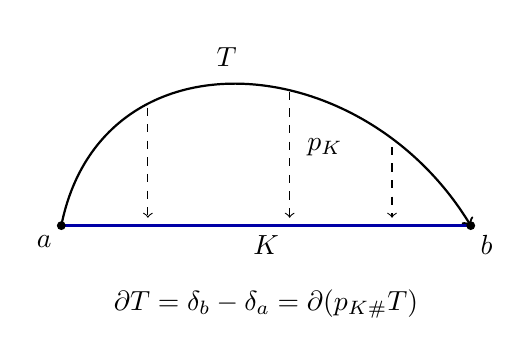
\begin{tikzpicture}[x=1cm,y=1cm]
	\draw[very thick,blue!65!black] (-2.6,0)--(2.6,0);
	\node[below] at (0,0) {\(K\)};
	\draw[thick,->] (-2.6,0) .. controls (-2.1,2.5) and (1.2,2.3) .. (2.6,0);
	\node[above] at (-0.5,1.9) {\(T\)};
	\draw[dashed,->] (-1.5,1.5)--(-1.5,0.1);
	\draw[dashed,->] (0.3,1.7)--(0.3,0.1);
	\draw[dashed,->] (1.6,1)--(1.6,0.1);
	\node[right] at (0.4,1) {\(p_K\)};
	\fill (-2.6,0) circle (1.6pt) node[below left] {\(a\)};
	\fill (2.6,0) circle (1.6pt) node[below right] {\(b\)};
	\node at (0,-1) {\(\partial T=\delta_b-\delta_a=\partial(p_{K\#}T)\)};
\end{tikzpicture}

	\caption[把竞争者投影到紧凸集]{把竞争者投影到紧凸集。图中以线段 \(K\) 和弧线示意一维情形；端点保持不动，弧线的推前落在 \(K\) 上。一般维数使用同一个 \(1\)-Lipschitz 估计控制质量。}
	\label{g3:fig:plateau-convex-projection}
\end{figure}

\subsection{极小化序列及质量界}
\label{g3:subsec:2301:04}
设 \(B\) 可填充，选定上述 \(K\)，并取一个初始竞争者 \(T_0\)。由下确界定义，对每个正整数 \(j\) 可选 \(R_j\in\mathcal A(B)\)，使
\[
	m(B)\le\mathbf M(R_j)\le m(B)+j^{-1}.
\]
令 \(T_j=p_{K\#}R_j\)。前一命题给出
\begin{equation}\label{g3:eq:plateau-minimizing-sequence}
\begin{aligned}
	&\operatorname{spt}T_j\subset K,\qquad \partial T_j=B,\\
	&m(B)\le\mathbf M(T_j)\le m(B)+j^{-1}
	\le\mathbf M(T_0)+1,\\
	&\mathbf N(T_j)=\mathbf M(T_j)+\mathbf M(B)
	\le\mathbf M(T_0)+1+\mathbf M(B).
\end{aligned}
\end{equation}
于是第22章紧性定理的全部条件已经具备：流为整数，支集共同紧，质量与边界质量有统一上界。边界质量之所以没有另外的估计困难，是因为竞争类从一开始就固定了整个边界流，而不只是边界所在的点集。

\ProseParagraphBreak
这种局部化思路见\cite[第34节，引理34.1及证明，第196--197页]{Simon1983}。这里把有限总质量但可能非紧支的竞争者也纳入比较，并显式核对投影对边界和整数性的作用。下一节从这列流出发，逐步识别极限及其质量。
% 纲要条目排为编号小节标题，并进入目录与书签；说明段仍保留于纲要注释中。

% !TeX root = ../../Book3.tex
% 纲要标题：### 23.2 整数流 Plateau 问题的存在性
% 纲要位置：几何学计划纲要.md，第 3082 行。
% 正文状态：初稿；尚未正式审核。

% 纲要内容开始
% 
% * 极小化序列的整数流极限
% * 边界算子的连续性
% * 质量下半连续
% * 极小填充的存在性
% * 极限中的拓扑变化
% 
% 纲要内容结束

\section{整数流 Plateau 问题的存在性}
\label{g3:sec:2302}
现在已有一列共同支于紧凸集的整数流，其质量趋于 \(m(B)\)，边界始终为 \(B\)。紧性给出极限对象；要把它认作解，还须分别检查它留在竞争类中以及它的质量达到下确界。把这两项检查分开，也能看清直接法在其他变分问题中需要哪些条件。

\subsection{极小化序列的整数流极限}
\label{g3:subsec:2302:01}
\begin{proposition}\label{g3:prop:plateau-limit-integer}
	设 \(1\le k\le n\)，\(B\in\mathcal I_{k-1}(\mathbb R^n)\) 紧支且可填充，\(K\) 为包含 \(\operatorname{spt}B\) 的非空紧凸集。由式\eqref{g3:eq:plateau-minimizing-sequence}选取的极小化序列有子列及 \(T_*\in\mathcal I_k(\mathbb R^n)\)，满足
	\[
		\operatorname{spt}T_*\subset K,\qquad
		\mathcal F(T_j-T_*)\longrightarrow0,
		\qquad T_j\rightharpoonup T_*.
	\]
\end{proposition}
\begin{proof}
	式\eqref{g3:eq:plateau-minimizing-sequence}给出共同紧支及
	\(\sup_j[\mathbf M(T_j)+\mathbf M(\partial T_j)]<\infty\)。逐项满足\cref{g3:thm:federer-fleming-compactness}的条件，所以有整数流子列极限及所述收敛。支集也可直接检查：若测试形式支于 \(\mathbb R^n\setminus K\)，每个 \(T_j\) 在其上均为零，故极限也为零。
\end{proof}

这里的整数性来自第22章已经证明的闭包定理。只对流的系数测度使用弱紧性，首先得到的是正规流；该步骤本身不会恢复可整流承载集和整数重数。前章关于切片的论证正好补齐了这部分。

\subsection{边界算子的连续性}
\label{g3:subsec:2302:02}
对任意 \(\eta\in\mathcal D^{k-1}(\mathbb R^n)\)，定义边界的公式给出
\begin{equation}\label{g3:eq:plateau-limit-boundary}
	\partial T_*(\eta)=T_*(\mathrm d\eta)
	=\lim_jT_j(\mathrm d\eta)
	=\lim_j\partial T_j(\eta)=B(\eta).
\end{equation}
因此 \(\partial T_*=B\)，极限确实属于 \(\mathcal A_K(B)\)。证明只用了 \(\mathrm d\eta\) 仍是紧支光滑测试形式，未要求边界在点集意义下逐点收敛。

\ProseParagraphBreak
例如，一列很薄的矩形边界可作为流趋于零，其支集却趋向一条非空线段。故“流的边界为 \(B\)”是一个有向积分恒等式，不能用“承载集的拓扑边界等于 \(\operatorname{spt}B\)”替换。整数流表示中的公共边可以因取向相反而抵消，重数也参与边界计算。

\subsection{质量下半连续}
\label{g3:subsec:2302:03}
若 \(\omega\) 为余质量至多一的紧支光滑 \(k\) 形式，则
\[
	T_*(\omega)=\lim_jT_j(\omega)\le\liminf_j\mathbf M(T_j).
\]
对 \(\omega\) 取上确界，即得\cref{g3:prop:current-mass-lsc}在此处的结论
\begin{equation}\label{g3:eq:plateau-limit-lsc}
	\mathbf M(T_*)\le\liminf_j\mathbf M(T_j)=m(B).
\end{equation}
另一方面，\(T_*\in\mathcal A(B)\) 使 \(m(B)\le\mathbf M(T_*)\)。两个方向合并后才得到质量相等。下半连续本身容许抵消损失，而极小化序列的极限仍属同一竞争类，使这种损失不能把质量降到下确界以下。

\begin{proposition}\label{g3:prop:plateau-minimizing-mass-measures}
	在上述极小化序列及其收敛子列下，有
	\[
		\mathbf M(T_j)\longrightarrow\mathbf M(T_*),\qquad
		\|T_j\|\rightharpoonup\|T_*\|
	\]
	作为支于 \(K\) 的有限 Radon 测度收敛。后一项指对每个连续函数的积分收敛，不表示 \(\mathbf M(T_j-T_*)\to0\)。
\end{proposition}
\begin{proof}
	总质量收敛已由下确界的两侧不等式得到。质量测度支于紧集 \(K\)，总量有界，所以任取子列都可再取弱收敛子列，记其极限为 \(\lambda\)。加权下半连续性说明，对每个非负紧支连续函数 \(\varphi\)，
	\[
		\int\varphi\,\mathrm d\|T_*\|\le\int\varphi\,\mathrm d\lambda.
	\]
	故 \(\lambda-\|T_*\|\) 是非负测度。取在 \(K\) 上等于一的 \(\varphi\)，总质量收敛又说明这个差测度的总量为零。因此 \(\lambda=\|T_*\|\)。任意子列的测度极限均相同，就得到整条已选流子列上的质量测度收敛。
\end{proof}

\subsection{极小填充的存在性}
\label{g3:subsec:2302:04}
\begin{theorem}[欧氏整数流 Plateau 存在性]\label{g3:thm:euclidean-plateau-existence}
	设 \(1\le k\le n\)，\(B\in\mathcal I_{k-1}(\mathbb R^n)\) 紧支，且存在有限质量整数流 \(T_0\in\mathcal I_k(\mathbb R^n)\) 满足 \(\partial T_0=B\)。则存在紧支整数流 \(T_*\in\mathcal I_k(\mathbb R^n)\)，使
	\begin{equation}\label{g3:eq:plateau-global-minimum}
		\partial T_*=B,\qquad
		\mathbf M(T_*)=\inf\{\mathbf M(S):
		S\in\mathcal I_k(\mathbb R^n),\ \partial S=B\}.
	\end{equation}
	若 \(B\ne0\)，可以取 \(\operatorname{spt}T_*\subset
	\overline{\operatorname{conv}}(\operatorname{spt}B)\)。若 \(B=0\)，唯一的质量极小者为零流。
\end{theorem}
\begin{proof}
	当 \(B=0\) 时，零流可容许，质量非负且质量为零当且仅当流为零，结论成立。以下设 \(B\ne0\)，取其支集的闭凸包为 \(K\)。它是非空紧凸集。

	初始竞争者使 \(0\le m(B)\le\mathbf M(T_0)<\infty\)。\cref{g3:prop:plateau-convex-reduction}将所有有限质量竞争者投影到 \(K\)，并证明受限前后的下确界相同。由式\eqref{g3:eq:plateau-minimizing-sequence}选择受限极小化序列，\cref{g3:prop:plateau-limit-integer}给出支于 \(K\) 的整数流极限 \(T_*\)。式\eqref{g3:eq:plateau-limit-boundary}保证 \(\partial T_*=B\)，式\eqref{g3:eq:plateau-limit-lsc}保证 \(\mathbf M(T_*)\le m(B)\)。最后用 \(T_*\) 本身的可容许性得到反向不等式，故 \(\mathbf M(T_*)=m(B)\)。下确界针对的是全部 \(\mathcal A(B)\)，所以极小性不限于支于 \(K\) 的竞争者。
\end{proof}

如果将 \(T_*\) 在一个有界开集内作紧支整数闭流扰动 \(Z\)，则 \(\partial(T_*+Z)=B\)，从而质量不会减小。更局部地，若 \(\operatorname{spt}Z\Subset W\)，在 \(W\) 外两流一致，减去相同的外部质量便有
\[
	\|T_*\|(W)\le\|T_*+Z\|(W).
\]
这就是后面内部正则性所需的局部绝对面积极小性质。定理没有给出一般的唯一性；证明中选取子列也允许不同极小化序列产生不同解。

\ProseParagraphBreak
为了计算一个确切最小值，把第19章的校准比较延伸到当前竞争类。那里“余范数”与第22章测试形式的“余质量”表示同一个 comass 范数。闭形式保持有向积分，余质量界将该积分与质量比较。

\begin{proposition}\label{g3:prop:euclidean-current-calibration}
	设 \(1\le k\le n\)，\(\phi\) 为 \(\mathbb R^n\) 上光滑闭 \(k\) 形式，处处满足 \(\|\phi_x\|_*\le1\)。若有限质量整数流
	\(T=\lBrack E,\tau,\theta\rBrack\)，其中 \(\theta>0\)，满足
	\(\langle\phi(x),\tau(x)\rangle=1\) 在 \(\|T\|\)-几乎处处成立，则对每个有限质量整数流 \(S\) 且 \(\partial S=\partial T\)，有 \(\mathbf M(T)\le\mathbf M(S)\)。
\end{proposition}
\begin{proof}
	有限质量流可以通过向量测度表示作用于有界光滑形式，所以 \(T(\phi)\)、\(S(\phi)\) 均有意义。先证明两者相等，并处理可能的非紧支集。

	径向同伦给出一个全局原始形式
	\[
		\alpha_x(v_1,\ldots,v_{k-1})
		=\int_0^1t^{k-1}\phi_{tx}(x,v_1,\ldots,v_{k-1})\,\mathrm dt,
		\qquad \mathrm d\alpha=\phi.
	\]
	最后一个等式由对拉回形式沿 \(x\mapsto tx\) 求导并在 \(t\in[0,1]\) 积分得到；正次数形式在常值映射下的拉回为零，闭性消去了含 \(\mathrm d\phi\) 的项。这也可逐个坐标系数使用乘积法则验证。余质量界给出 \(\|\alpha_x\|_*\le |x|/k\)。

	令 \(Q=S-T\)，则 \(\partial Q=0\)。取前节所用 \(\chi_R\)，边界恒等式给出
	\[
		0=Q(\mathrm d(\chi_R\alpha))
		=Q(\chi_R\phi)+Q(\mathrm d\chi_R\wedge\alpha).
	\]
	第二项的绝对值不超过
	\(C_{n,k}\|Q\|(B_{2R}\setminus B_R)\)，因为该环域上 \(|\mathrm d\chi_R|\le C/R\)、\(\|\alpha\|_*\le2R/k\)。有限总质量使这个上界趋于零。第一项由控制收敛趋于 \(Q(\phi)\)，故 \(S(\phi)=T(\phi)\)。于是
	\[
		\mathbf M(T)=T(\phi)=S(\phi)\le\mathbf M(S).
	\]
	这证明了对全体有限质量竞争者的比较。
\end{proof}

在\cref{g3:exm:plateau-disk-initial}中，取常系数形式
\(\phi=\mathrm dx_1\wedge\mathrm dx_2\)，得到 \(m(B)=\pi R^2\)；边界为 \(qB\) 时，按 \(q\) 的正负选择 \(\phi\) 或 \(-\phi\)，得到 \(m(qB)=|q|\pi R^2\)。同样，对于两个不同点 \(a,b\)，常系数一形式
\(\phi=\langle(b-a)/|b-a|,\mathrm dx\rangle\) 校准从 \(a\) 到 \(b\) 的线段，故
\[
	m(\delta_b-\delta_a)=|b-a|.
\]
这些下界比较的是所有整数流竞争者，而不是只比较光滑图形。

\subsection{极限中的拓扑变化}
\label{g3:subsec:2302:05}
取 \(\mathbb R^3\) 中的单位圆盘 \(D\)，并在它上方放置半径 \(\varepsilon\) 的球面 \(S_\varepsilon\)，球心为 \((0,0,3\varepsilon)\)。两个承载集不相交。按各自取向令
\[
	T_\varepsilon=\lBrack D\rBrack+\lBrack S_\varepsilon\rBrack.
\]
则
\[
	\partial T_\varepsilon=\partial\lBrack D\rBrack,\qquad
	\mathbf M(T_\varepsilon)=\pi+4\pi\varepsilon^2\longrightarrow\pi,
\]
且球体填充给出
\(\mathcal F(T_\varepsilon-\lBrack D\rBrack)\le4\pi\varepsilon^3/3\)。这是一列极小化序列，其闭球面分支在极限中消失。固定边界并没有固定分支数。

\ProseParagraphBreak
即使要求曲面连通，细把手也可消失。具体地，在一个固定平面圆片内部去掉两个小圆盘，用上半空间中一条弧线的细管把两个圆周连接，再在接缝处光滑倒圆，得到与原圆片在外缘邻域一致的嵌入定向曲面。弧线可取半圆，管半径取为其半径的十分之一；管壁与外侧平面之间的两个直角接缝用固定光滑截面连接。这样得到一个具有有限面积的固定模型，外缘不动，内部增加一个把手。

\ProseParagraphBreak
把该模型按比例 \(\varepsilon\) 缩小，替换 \(D\) 内部半径 \(C\varepsilon\) 的圆片，记所得曲面为 \(D_\varepsilon\)。它仍连通，边界仍是单位圆，亏格增加一。修改只发生在直径 \(O(\varepsilon)\) 的区域，且新旧两片面积都为 \(O(\varepsilon^2)\)，故
\[
	\mathbf M(\lBrack D_\varepsilon\rBrack-\lBrack D\rBrack)
	\le C'\varepsilon^2,\qquad
	\mathbf M(\lBrack D_\varepsilon\rBrack)\longrightarrow\pi.
\]
所以固定亏格的光滑竞争者也可能收敛到不同亏格的流。Plateau 存在性保留的是定义中指定的整数结构与边界条件；拓扑约束是否保留，要在相应的更小竞争类中单独研究。

\ProseParagraphBreak
最后，质量相等也不会把平坦收敛加强为质量范数收敛。令 \(G_\varepsilon\) 为单位圆盘上函数 \(u_\varepsilon(x)=\varepsilon(1-|x|^2)\) 的向上定向图，则边界固定，面积趋于 \(\pi\)。图面在圆盘内部与 \(D\) 不交，而边界的一维集合没有二维质量，因此
\[
	\mathbf M(\lBrack G_\varepsilon\rBrack-\lBrack D\rBrack)
	=\mathbf M(\lBrack G_\varepsilon\rBrack)+\pi\longrightarrow2\pi.
\]
两者之间的竖向同伦却有质量 \(O(\varepsilon)\)，且侧边固定，故其平坦距离趋于零。这与\cref{g3:prop:plateau-minimizing-mass-measures}的质量测度弱收敛完全相容。
% 纲要条目排为编号小节标题，并进入目录与书签；说明段仍保留于纲要注释中。

% !TeX root = ../../Book3.tex
% 纲要标题：### 23.3 单调性、切锥与正则点
% 纲要位置：几何学计划纲要.md，第 3090 行。
% 正文状态：初稿；尚未正式审核。

% 纲要内容开始
% 
% * 第一变分和驻值
% * 密度及放大极限
% * 平面切锥与正则性问题
% * 极小整数流的内部与边界正则性
% 
% 纲要内容结束

\section{单调性、切锥与正则点}
\label{g3:sec:2303}
极小化给出一个整数流之后，还要辨认它在小尺度上的形状。可以先用光滑微分同胚移动这个流；极小性使质量的一阶变化为零，径向移动进而比较同一中心的不同尺度。缩小观察尺度得到切锥，它保留面积密度与重数。最后需要正则性定理，把足够平坦的弱对象恢复成光滑曲面。本节完整推导第一变分和单调性；极小流的质量收敛以及一般正则性采用下文逐项注明的外部结果。

\subsection{第一变分和驻值}
\label{g3:subsec:2303:01}
设 \(U\subset\mathbb R^n\) 开，\(1\le k<n\)。本节的局部质量极小，是指局部整数 \(k\) 流 \(T\) 满足：对每个 \(W\Subset U\) 及支于 \(W\) 内某个紧集的整数 \(k\) 流 \(Z\)，只要 \(\partial Z=0\)，就有
\[
	\|T\|(W)\le\|T+Z\|(W).
\]
由前节得到的全空间固定边界极小流满足这个条件。下面只在 \(U\cap\operatorname{spt}\partial T=\varnothing\) 的区域讨论内部变分。

\ProseParagraphBreak
将 \(T\) 写成 \(\lBrack E,\tau,\theta\rBrack\)，其中 \(\theta\) 取正整数，取向的符号吸收到 \(\tau\) 中。记 \(P_x\) 为 \(E\) 在几乎每点的近似切平面，\(\mu=\|T\|=\theta\mathcal H^k\llcorner E\)。对 \(C^1\) 向量场 \(X\)，定义沿 \(P_x\) 的散度
\[
	\operatorname{div}_{P_x}X
	=\sum_{i=1}^k\langle \mathrm DX(x)e_i,e_i\rangle,
\]
其中 \(e_1,\ldots,e_k\) 是 \(P_x\) 的任意正交单位基。它是 \(\mathrm DX\) 在该平面上的迹，因而不依赖基的选择。

\begin{theorem}\label{g3:thm:minimizing-current-stationarity}
	设 \(T\) 是开集 \(U\subset\mathbb R^n\) 中局部质量极小的整数 \(k\) 流，\(\partial T=0\) 于 \(U\)，\(1\le k<n\)。记 \(\mu=\|T\|\)，\(P_x\) 为其可整流表示的近似切平面，\(\operatorname{div}_{P_x}\) 为切向散度。则对每个 \(X\in C_c^1(U;\mathbb R^n)\)，都有
	\begin{equation}\label{g3:eq:current-stationarity}
		\delta T(X)\coloneqq\int\operatorname{div}_{P_x}X\,\mathrm d\mu(x)=0.
	\end{equation}
\end{theorem}
\begin{proof}
	先取光滑 \(X\)，令 \(\Phi_t\) 为它的小时间流。选 \(W\Subset U\)，使 \(X\) 的支集紧含于 \(W\)。\(\Phi_t\) 在 \(W\) 边界附近为恒等。第22章的推前与同伦公式说明 \(\Phi_{t\#}T-T\) 紧支于 \(W\)，其边界为零，故是允许的局部竞争变化。

	微分同胚单射，推前时没有不同原像之间的取向抵消。\cref{g3:prop:rectifiable-lipschitz-pushforward}的面积公式于是给出
	\[
		\|\Phi_{t\#}T\|(W)
		=\int_{E\cap W}J_k(\mathrm D\Phi_t|_{P_x})\,\theta\,\mathrm d\mathcal H^k.
	\]
	在 \(P_x\) 的正交基下，Jacobian 是 Gram 行列式的平方根。由
	\(\mathrm D\Phi_t=I+t\mathrm DX+o(t)\)，得到
	\[
		\left.\frac{\mathrm d}{\mathrm dt}\right|_{t=0}
		J_k(\mathrm D\Phi_t|_{P_x})
		=\sum_{i=1}^k\langle\mathrm DXe_i,e_i\rangle.
	\]
	余项在包含 \(\operatorname{spt}X\) 的紧集以及全部 \(k\) 平面上均匀；局部质量有限允许在积分号下求导。正负 \(t\) 都是竞争参数，极小性迫使导数为零，得到式\eqref{g3:eq:current-stationarity}。最后用同一紧支集上的光滑 \(C^1\) 逼近推广到 \(C_c^1\) 向量场。
\end{proof}

我们把满足式\eqref{g3:eq:current-stationarity}的可整流质量分布称为\term[zhuzhi]{驻值}[stationary]的。这个条件只使用 \(P_x\) 与正质量 \(\mu\)，不使用切平面的取向。若 \(E\) 是光滑无边界子流形，它恢复第19章的面积驻值公式：本书光滑平均曲率 \(H\) 是第二基本形式迹的 \(1/k\)，所以
\(\delta T(X)=-k\int\langle H,X\rangle\,\mathrm d\mu\)
在重数局部常值的区域成立。驻值是一阶条件；它不自动给出任意竞争流的质量比较。

\subsection{密度及放大极限}
\label{g3:subsec:2303:02}
取向消失于第一变分之后，径向计算与光滑情形具有同一形式。所需的是几乎处处的切平面，不需要先知道支集是一张光滑曲面。

\begin{theorem}\label{g3:thm:stationary-current-monotonicity}
	设 \(T\) 为 \(U\subset\mathbb R^n\) 中局部整数 \(k\) 流，\(1\le k<n\)，记 \(\mu=\|T\|\)、\(P_x\) 为近似切平面，并假定其质量分布满足式\eqref{g3:eq:current-stationarity}。若 \(\overline B_R(a)\subset U\)，则
	\[
		r\longmapsto\frac{\mu(B_r(a))}{r^k}
	\]
	在 \((0,R)\) 上单调不减。对满足
	\(\mu(\partial B_s(a))=\mu(\partial B_t(a))=0\)
	的 \(0<s<t<R\)，有精确差值式
	\begin{equation}\label{g3:eq:current-monotonicity-difference}
		\frac{\mu(B_t(a))}{t^k}-\frac{\mu(B_s(a))}{s^k}
		=\int_{B_t(a)\setminus B_s(a)}
		\frac{|(x-a)^{\perp P_x}|^2}{|x-a|^{k+2}}\,\mathrm d\mu(x).
	\end{equation}
\end{theorem}
\begin{proof}
	平移后取 \(a=0\)。令 \(r=|x|\)，先在径向光滑截断
	\(X(x)=\gamma(r)x\) 中计算。因为
	\(\sum_i\langle x,e_i\rangle^2=|x^{P_x}|^2\)，有
	\[
		\operatorname{div}_{P_x}X
		=k\gamma(r)+r\gamma'(r)
		-\frac{\gamma'(r)}r|x^{\perp P_x}|^2.
	\]
	选择如下连续、分段光滑的截断：
	\[
		\gamma(r)=
		\begin{cases}
			s^{-k}-t^{-k},&0\le r\le s,\\
			r^{-k}-t^{-k},&s<r<t,\\
			0,&r\ge t.
		\end{cases}
	\]
	它在原点附近为常数。只在 \(s,t\) 附近作光滑化，函数及其导数保持一致有界；由于两个球面的 \(\mu\) 质量为零，可用控制收敛将它代入驻值等式。\(r<s\) 的散度是 \(k(s^{-k}-t^{-k})\)；\(s<r<t\) 上的散度是
	\(-kt^{-k}+k|x^{\perp P_x}|^2r^{-k-2}\)。积分相加，再除以 \(k\)，便得到式\eqref{g3:eq:current-monotonicity-difference}。

	右侧非负，故质量比在这些良好半径之间单调。坏半径至多可数，因为不同球面互不相交，而 \(\mu\) 在 \(B_R(a)\) 内有限。对任意 \(s<t\)，分别取良好半径从下方趋于 \(s,t\)；开球递增并覆盖目标开球，测度的下连续性遂把单调性推广到全部半径。
\end{proof}

\begin{corollary}\label{g3:cor:minimizing-current-density}
	设 \(U\subset\mathbb R^n\) 开，\(1\le k<n\)，\(T\) 为 \(U\) 中局部整数 \(k\) 维流，\(\mu=\|T\|\)，且 \(\int\operatorname{div}_{P_x}X\,\mathrm d\mu=0\) 对所有 \(X\in C_c^1(U;\mathbb R^n)\) 成立；这里 \(P_x\) 为近似切平面，\(\theta\) 为整数重数。则每个 \(a\in U\) 都存在有限密度
	\[
		\Theta^k(\mu,a)
		=\lim_{r\downarrow0}\frac{\mu(B_r(a))}{\omega_kr^k}.
	\]
	在 \(\mu\)-几乎每点，此密度等于整数重数 \(\theta(a)\)。若 \(a\in\operatorname{spt}T\)，则 \(\Theta^k(\mu,a)\ge1\)。特别地，在球不遇 \(U\) 边界时，
	\begin{equation}\label{g3:eq:stationary-integer-mass-lower-bound}
		\mu(B_r(a))\ge\omega_kr^k.
	\end{equation}
\end{corollary}
\begin{proof}
	单调性使质量比在趋零时有极限，其值不超过任意固定内球的有限质量比。\cref{g3:thm:weighted-rectifiable-density}适用于整数重数表示：\(\theta\ge1\) 使载体在局部具有有限 \(\mathcal H^k\) 测度，所以几乎处处的密度是 \(\theta\)。

	这些密度至少为一的点在支集中稠密。给定 \(a\in\operatorname{spt}T\)，取这样的点 \(a_j\to a\)。对固定 \(r\) 及充分大的 \(j\)，球
	\(B_{r-|a_j-a|}(a_j)\) 包含于 \(B_r(a)\)。在 \(a_j\) 处使用单调性和密度下界，再令 \(j\to\infty\)，得到式\eqref{g3:eq:stationary-integer-mass-lower-bound}。最后令 \(r\downarrow0\)。
\end{proof}

现在固定内部点 \(a\in\operatorname{spt}T\)，用
\[
	\eta_{a,r}(x)=\frac{x-a}{r},\qquad T_{a,r}=\eta_{a,r\#}T
\]
放大。推前本身已含 \(k\) 阶 Jacobian，质量满足
\(\|T_{a,r}\|(B_R)=r^{-k}\mu(B_{Rr}(a))\)，不再另乘 \(r^{-k}\)。对每个固定 \(R\)，单调性给出这些质量的一致上界，而充分小的 \(r\) 使放大流在 \(B_R\) 中无边界。\cref{g3:thm:local-integral-current-compactness}因此给出局部整数弱极限。

\ProseParagraphBreak
要把它称作切锥，还需要防止质量在弱极限中抵消。这里调用极小流特有的紧性加强，其证明通过切片粘合小误差，使极限的竞争者能转移回原序列。精确外部输入如下；来源是\cite[定理34.5及注34.6(1)，第198--202页]{Simon1983}。

\begin{theorem}\label{g3:thm:minimizing-current-mass-compactness}
	设 \(U\subset\mathbb R^n\) 开，\(T_j\) 为 \(U\) 中局部质量极小的整数 \(k\) 流，\(\partial T_j=0\) 于 \(U\)。若它们在每个 \(W\Subset U\) 上质量一致有界，并且 \(T_j\rightharpoonup T\)，则 \(T\) 仍局部质量极小且为整数流，并有
	\[
		\|T_j\|\rightharpoonup\|T\|
	\]
	作为局部 Radon 测度收敛。
\end{theorem}

上述定理在此作为外部结果使用。它比第22章的整数流紧性多给出质量测度收敛与极小性的保持；单独的下半连续性没有这些结论。位置与切平面的联合测度将在\secref{g3:sec:2304}中正式定义为变分流形。

\begin{theorem}\label{g3:thm:minimizing-current-tangent-cone}
	设 \(T\) 是 \(U\subset\mathbb R^n\) 中局部质量极小的整数 \(k\) 流，\(\partial T=0\) 于 \(U\)，\(1\le k<n\)。记 \(T_{a,r}=(x\mapsto(x-a)/r)_\#T\)。给定 \(a\in\operatorname{spt}T\) 和任意 \(r_j\downarrow0\)，可取子列使 \(T_{a,r_j}\rightharpoonup C\) 局部收敛，其中 \(C\ne0\) 是 \(\mathbb R^n\) 中局部质量极小、无边界的整数流，满足
	\begin{equation}\label{g3:eq:current-tangent-cone-homogeneity}
		D_{\lambda\#}C=C\quad(\lambda>0),\qquad D_\lambda(x)=\lambda x,
	\end{equation}
	以及
	\[
		\|C\|(B_R)=\omega_kR^k\Theta^k(\|T\|,a)\quad(R>0).
	\]
	这样的 \(C\) 称为 \(T\) 在 \(a\) 的\term[qiezhui]{切锥}[tangent cone]。
\end{theorem}
\begin{proof}
	前述局部质量界与整数紧性先给出 \(C\)。每个放大流仍在相应放大开集内质量极小；对任意固定球，充分大的 \(j\) 都满足外部定理的假设。逐球使用\cref{g3:thm:minimizing-current-mass-compactness}，知 \(C\) 极小，且质量测度局部收敛。

	当 \(\|C\|(\partial B_R)=0\) 时，测度收敛给出
	\[
		\|C\|(B_R)
		=\lim_jr_j^{-k}\mu(B_{Rr_j}(a))
		=\omega_kR^k\Theta^k(\mu,a).
	\]
	这样的半径除至多可数个外任意。由良好半径从两侧逼近，知这个等式对全部 \(R>0\) 成立，且所有球面均为 \(\|C\|\) 零测集。密度下界保证 \(C\ne0\)。

	\(C\) 是驻值的，且其质量比恒定。将差值式\eqref{g3:eq:current-monotonicity-difference}用于 \(C\)，得到
	\(x\in P_x\) 在 \(\|C\|\)-几乎处处成立。这还须转成流本身的齐次性。固定 \(\lambda>0\)，考虑
	\(F(t,x)=(1-t+t\lambda)x\)，\(0\le t\le1\)。时间方向的导数是 \((\lambda-1)x\)，已在切平面内，因此 \(F\) 作用于 \([0,1]\times C\) 的 \((k+1)\) 维切向 Jacobian 为零。推前流因而为零。又 \(\partial C=0\)，同伦公式给出
	\[
		D_{\lambda\#}C-C
		=\partial F_\#([0,1]\times C)=0.
	\]
	这里缩放因子始终处于两个正数之间；对任意紧支测试形式，其逆像支集仍有界，故第22章的局部同伦公式适用。齐次性得证。
\end{proof}

这个结论保证每个放大序列都有切锥子列，未指定不同子列必有同一极限。切锥保留中心密度，却可能比原流的局部几何简单得多；下一小节的分支曲线正体现这一点。

\subsection{平面切锥与正则性问题}
\label{g3:subsec:2303:03}
称内部点 \(a\in\operatorname{spt}T\) 为正则点，是指某个邻域内
\(T=q\lBrack M\rBrack\)，其中 \(M\) 是光滑嵌入、无边界、定向的 \(k\) 维子流形，\(q\) 为正整数。其余内部支集点组成奇异集 \(\operatorname{Sing}_{\mathrm{int}}T\)。正则性描述支集和重数的局部表示，单独出现一张平面作为切锥还没有提供这种表示。

\ProseParagraphBreak
重数为一时，Allard\footnote{William Kenneth Allard（1941—），在美国工作的数学家，研究几何测度论，建立了变分流形的第一变分与正则性理论。}正则性给出明确结论。下面是其驻值整数流特例，作为外部正则性结果引用\cite[定理24.2，第125--128页；定理36.3，第211--212页]{Simon1983}；含 \(L^p\) 平均曲率的定量输入见\cref{g3:thm:allard-regularity}。

\begin{theorem}\label{g3:thm:unit-density-minimizing-current-regularity}
	设 \(T\) 是开集 \(U\subset\mathbb R^n\) 中局部质量极小、无边界的整数 \(k\) 流。若 \(a\in\operatorname{spt}T\) 满足
	\(\Theta^k(\|T\|,a)=1\)，则 \(a\) 是重数为一的正则点。特别地，若某个切锥是重数为一的定向平面流，则 \(a\) 正则。
\end{theorem}

说明调用条件如何出现：整数重数使几乎处处密度至少为一，驻值性使广义平均曲率为零，而中心密度为一使充分小球上的质量比任意接近一。Allard 定理把这三个条件变成一张 \(C^{1,\alpha}\) 单图；把流沿图投影推到参数平面，无边界条件与\cref{g3:thm:current-constancy}使所得顶维流的整数重数为常数；再沿图嵌入推回，并用中心密度为一确定该常数。在 Euclid 极小图方程下，局部椭圆正则性将它提升为光滑图。若从平面切锥出发，则上一小节的质量测度收敛先保证中心密度确为一。这个质量信息是把弱放大极限用于正则性判断的关键。

\begin{example}\label{g3:exm:complex-cusp-current}
	在 \(\mathbb C^2\cong\mathbb R^4\) 中取
	\[
		F(z)=(z^2,z^3),\qquad T=F_\#\lBrack\overline D\rBrack,
	\]
	其中 \(D\subset\mathbb C\) 为单位圆盘，取复定向。\(F\) 光滑，在 \(z\ne0\) 时是单射浸入：若 \(z^2=w^2\) 且 \(z^3=w^3\)，则 \(z=w\)。故 \(T\) 在原点之外的有效重数为一，边界是光滑嵌入曲线 \(F(\partial D)\)。

	标准二形式
	\(\omega=\mathrm dx_1\wedge\mathrm dy_1+\mathrm dx_2\wedge\mathrm dy_2\)
	由\cref{g3:prop:wirtinger-calibration}具有余质量一，并在每个正向复直线上取等。\(F\) 的非退化切平面均为复直线，故 \(T(\omega)=\mathbf M(T)\)。这个形式全局光滑、有界且闭，因此\cref{g3:prop:euclidean-current-calibration}适用，说明 \(T\) 在全部有限质量、同整数边界的竞争者中质量最小，特别地局部质量极小。

	令 \(b>0\) 满足 \(r^2=b^4+b^6\)。因为
	\(J_2F(z)=4|z|^2+9|z|^4\)，对充分小的 \(r\) 有
	\[
		\|T\|(B_r(0))
		=\int_{|z|<b}(4|z|^2+9|z|^4)\,\mathrm d\mathcal L^2(z)
		=2\pi b^4+3\pi b^6.
	\]
	所以 \(\Theta^2(\|T\|,0)=2\)。将参数改写为 \(z=\sqrt r\,w\)，放大后的参数化为
	\[
		w\longmapsto(w^2,\sqrt r\,w^3).
	\]
	任意固定紧支测试形式的原像位于一致有界的 \(w\) 域；参数化在该域光滑收敛到 \(w\mapsto(w^2,0)\)。于是全部放大流都趋于 \(2\lBrack\mathbb C\times\{0\}\rBrack\)，它是唯一的平面切锥。

	然而原点不是正则点。若支集在原点附近是 \(C^1\) 嵌入曲面，其切平面必为 \(\mathbb C\times\{0\}\)，到第一复坐标的投影将由逆函数定理局部单射。但 \(F(z)\) 与 \(F(-z)\) 在 \(z\ne0\) 时是不同点，却有相同的第一坐标 \(z^2\)，矛盾。这个例子同时具有质量极小性、光滑边界和唯一平面切锥，仍在内部出现分支奇点。
\end{example}

\subsection{极小整数流的内部与边界正则性}
\label{g3:subsec:2303:04}
密度一正则性处理最接近平面的单层情形。一般内部奇异集的大小还取决于维数与余维，尤其不能把超曲面的维数阈值用于高余维流。以下两项是本节采用的外部内部正则性结论。

\begin{theorem}\label{g3:thm:area-minimizing-interior-singular-bounds}
	设 \(U\subset\mathbb R^n\) 开，\(2\le k<n\)，\(T\) 为 \(U\) 中局部质量极小的整数 \(k\) 流，\(\partial T=0\) 于 \(U\)。
	\begin{enumerate}
		\item 在任意余维中，\(\operatorname{Sing}_{\mathrm{int}}T\) 的 Hausdorff 维数至多为 \(k-2\)，即对每个 \(\varepsilon>0\)，
		\[
			\mathcal H^{k-2+\varepsilon}(\operatorname{Sing}_{\mathrm{int}}T)=0.
		\]
		\item 若 \(n=k+1\)，则 \(k\le6\) 时内部无奇点；\(k=7\) 时内部奇异集局部有限；\(k\ge8\) 时其 Hausdorff 维数至多为 \(k-7\)。
	\end{enumerate}
\end{theorem}

第一项是 Almgren\footnote{Frederick Justin Almgren Jr.（1933--1997），美国数学家，主要研究几何测度论。}的一般内部正则性定理，此处采用\cite[第36节，第210--211页]{Simon1983}所陈述的 Euclid 特例，证明依赖多值函数及分支分析。第二项见\cite[第37节，尤其定理37.7及其证明，第215--223页]{Simon1983}；书中先证明局部有限周长集合边界的版本，再通过余维一极小整数流的局部分层分解处理整数重数。高重数分层的最大值原理以及维数降低是这项结论的组成部分，不能只把一般流直接认作一个集合的边界。

\ProseParagraphBreak
这里 \(k\) 是流的维数。例如二维整数流在 \(\mathbb R^3\) 中内部光滑；在 \(\mathbb R^4\) 中，一般结论只把内部奇异集的 Hausdorff 维数压到零，\cref{g3:exm:complex-cusp-current}确实出现一个奇点。维数为零本身不意味着集合局部有限，后一个更强断言需要另行给出对应定理。

\ProseParagraphBreak
边界正则性另有假设。我们选用如下余维一版本，外引 Hardt--Simon\footnote{Robert M. Hardt，在美国工作的数学家，研究几何测度论与偏微分方程。Leon Melvyn Simon（1945—），澳大利亚出生的数学家，研究极小曲面、几何测度论与偏微分方程。}的边界正则性定理；正式公告明确陈述于\cite[定理2，第263--264页]{HardtSimon1979BoundaryAnnouncement}。

\begin{theorem}\label{g3:thm:hardt-simon-boundary-regularity}
	设 \(U\subset\mathbb R^{k+1}\) 开，\(k\ge2\)，\(T\) 是 \(U\) 中局部绝对质量极小的整数 \(k\) 流。设在 \(U\) 中
	\[
		\partial T=\lBrack\Gamma\rBrack,
	\]
	其中 \(\Gamma\) 为无边界、定向、嵌入的 \(C^2\) \((k-1)\) 维子流形，系数为一。则存在 \(\Gamma\) 的开邻域 \(V\subset U\)，使 \(V\cap\operatorname{spt}T\) 局部为嵌入的 \(C^{1,\alpha}\) 超曲面，对每个 \(0<\alpha<1\) 成立。支集可在 \(\Gamma\) 处终止，也可穿过 \(\Gamma\)；在后一种情形，\(\Gamma\) 两侧的整数重数跳跃一。若 \(\Gamma\) 光滑，则边界处的表示也光滑。
\end{theorem}

本定理的绝对质量极小，仍按本节开始的紧支整数闭流竞争定义，而非只对光滑微分同胚驻值。它的边界是重数一的嵌入子流形，环境余维为一。穿越情形可从两个同向同心平面圆周看出：相应平面填充在内圆盘上重数为二、外环带上重数为一，内圆是流的边界所在，但支集在那里是一整张平面。因此“边界正则”不要求支集的拓扑边界处处等于 \(\operatorname{spt}\partial T\)。

\ProseParagraphBreak
高余维的边界即使局部光滑，也可能遇到其他极小片。例如在 \(\mathbb C^2\) 中，把第一复坐标平面上的半圆盘流与第二复坐标平面上的整圆盘流相加，并在原点附近观察。边界在那里只是一条光滑直线，两个复片都由同一个 \(\omega\) 校准，故和流局部质量极小；原点附近支集却是相交的两片，不能表示成一张嵌入带边界曲面。此例说明余维一边界定理的环境条件有实际作用。对于给定 Plateau 解，内部结论应在远离边界处使用，边界结论则逐点核查所选定理的边界重数、嵌入性与环境条件。
% 纲要条目排为编号小节标题，并进入目录与书签；说明段仍保留于纲要注释中。

% !TeX root = ../../Book3.tex
% 纲要标题：### 23.4* 变分流形与第一变分
% 纲要位置：几何学计划纲要.md，第 3097 行。
% 正文状态：初稿；尚未正式审核。

% 纲要内容开始
% 
% * Grassmann 丛上的测度
% * 一阶变分和广义平均曲率
% * 无取向极限及重数
% * 流与变分流形的边界及抵消
% * Allard 正则性定理
% 
% ---
% 
% 纲要内容结束

\OptionalSection{变分流形与第一变分}{g3:sec:2304}

取两张彼此靠近、取向相反的平面。它们作为流可以相消，面积却仍是两张平面的面积。如果研究的目标是面积的驻值及其极限，就需要保留位置、面积和切平面，而不让取向改变面积的符号。变分流形用 Grassmann 丛上的正测度实现这一点。这里先建立测度与变分的基本运算，再准确陈述把弱几何对象恢复为图像的 Allard 正则性定理。一般变分流形的定义和第一变分参见\cite[第38--39节，第227--235页]{Simon1983}；其中 Grassmann 丛上的弱收敛有别于该书第15节仅对权测度所用的收敛约定。

\subsection{Grassmann 丛上的测度}
\label{g3:subsec:2304:01}
设 \(U\subset\mathbb R^n\) 开，\(1\le k<n\)。记 \(G(n,k)\) 为 \(\mathbb R^n\) 中所有\emph{无取向}的 \(k\) 维线性子空间组成的 Grassmann 流形。把平面 \(P\) 与其正交投影矩阵 \(\pi_P\) 对应，则
\[
	G(n,k)=\{A\in\mathbb R^{n\times n}:A^{\mathsf T}=A,\ A^2=A,\ \operatorname{tr}A=k\}.
\]
这是矩阵空间中的闭有界集，因而紧。距离可取 \(|\pi_P-\pi_Q|\)。Euclid 情形的 Grassmann 丛是乘积
\[
	G_k(U)\coloneqq U\times G(n,k).
\]
其一点 \((x,P)\) 同时记录位置和经过该位置的平面方向；仿射切平面对应 \(x+P\)。

\begin{definition}\label{g3:def:varifold}
	设 \(U\subset\mathbb R^n\) 开，\(1\le k<n\)。记 \(G(n,k)\) 为 \(\mathbb R^n\) 的无取向 \(k\) 平面空间，\(G_k(U)=U\times G(n,k)\)。\(G_k(U)\) 上的非负 Radon 测度称为 \(U\) 中的 \(k\) 维\term[bianfen liuxing]{变分流形}[varifold]，记为 \(V\)。其\term[quanzhong cedu]{权测度}[weight measure]是位置投影 \(\pi(x,P)=x\) 的推前
	\[
		\mu_V(A)\coloneqq V(A\times G(n,k)),\qquad A\subset U\text{ 为 Borel 集}.
	\]
	权测度也记为 \(\|V\|\)。总质量为 \(\mu_V(U)\)，在环境中的支集指 \(\operatorname{spt}\mu_V\)。
\end{definition}
\symidx{\(\mu_V=\lVert V\rVert\)：变分流形的权测度}

Grassmann 纤维紧，故紧集 \(K\Subset U\) 的逆像 \(K\times G(n,k)\) 也紧，权测度在 \(U\) 上确为 Radon 测度。定义中的“变分”不表示已经满足某个极值条件；任意这样的非负测度都是变分流形。

\begin{definition}\label{g3:def:rectifiable-varifold}
	设 \(U\subset\mathbb R^n\) 开，\(1\le k<n\)，\(G_k(U)=U\times G(n,k)\) 为无取向切平面丛，\(M\subset U\) 是可数 \(k\)-可整流 Borel 集，\(\theta:M\to(0,\infty)\) 可测，并且 \(\int_{M\cap K}\theta\,\mathrm d\mathcal H^k<\infty\) 对每个 \(K\Subset U\) 成立。按 Lipschitz 片取几乎处处一致的切平面 \(\mathrm{T}_xM\)，以
	\begin{equation}\label{g3:eq:rectifiable-varifold}
		\mathbf v(M,\theta)(\varphi)
		=\int_M\varphi(x,\mathrm{T}_xM)\theta(x)\,\mathrm d\mathcal H^k(x),
		\qquad \varphi\in C_c(G_k(U)),
	\end{equation}
	定义的变分流形称为\term[kezhengliu bianfen liuxing]{可整流变分流形}[rectifiable varifold]。如果 \(\theta\) 几乎处处取正整数值，就称为\term[zheng bianfen liuxing]{整变分流形}[integral varifold]。重数为一时简记 \(\mathbf v(M)\)。
\end{definition}
\symidx{\(\mathbf v(M,\theta)\)：由可整流集及正重数定义的变分流形}

一般实重数可使整个承载集的局部 \(\mathcal H^k\) 测度无限；此时切平面按可数片确定，沿用\cref{g3:def:rectifiable-current}的约定。整数重数满足 \(\theta\ge1\)，于是有效承载集局部 \(\mathcal H^k\) 有限。式\eqref{g3:eq:rectifiable-varifold}给出
\[
	\mu_{\mathbf v(M,\theta)}=\theta\mathcal H^k\llcorner M.
\]
可整流流 \(T=\lBrack M,\tau,\theta\rBrack\) 所对应的变分流形记为
\begin{equation}\label{g3:eq:current-associated-varifold}
	V_T\coloneqq\mathbf v(M,|\theta|),\qquad \mu_{V_T}=\|T\|.
\end{equation}
这一构造忘掉 \(\tau\) 的正负，但保留其张成的平面。一个嵌入的 Möbius 带也直接给出 \(\mathbf v(M)\)，无需选择全局取向。

\begin{example}\label{g3:exm:diffuse-varifold}
	设 \(U\subset\mathbb R^n\) 为非空开集。取 \(1\le k<n\) 和两个不同平面 \(P,Q\in G(n,k)\)。测度
	\[
		V_P=\mathcal L^n\llcorner U\otimes\delta_P,\qquad
		V_Q=\mathcal L^n\llcorner U\otimes\delta_Q
	\]
	有相同权测度，却是不同的变分流形，因为可以用只依赖平面方向的连续函数区别它们。两者均非 \(k\) 维可整流：可数 \(k\)-可整流集的 \(n\) 维 Lebesgue 测度为零，无法承载 \(\mathcal L^n\llcorner U\)。所以权测度和维数标记本身不保证切向几何结构。
\end{example}

为比较变形前后的面积，推前还必须带上切向 Jacobian。设 \(f:U\to W\subset\mathbb R^q\) 为 \(C^1\) 映射，且在 \(\operatorname{spt}\mu_V\) 上对 \(W\) 固有。定义
\[
	J_Pf(x)=\sqrt{\det\bigl((\mathrm Df(x)|_P)^*\mathrm Df(x)|_P\bigr)}.
\]
这里假设 \(q\ge k\)。当此数非零时，\(\mathrm Df(x)P\) 是 \(k\) 维平面。令
\begin{equation}\label{g3:eq:varifold-pushforward}
	(f_\#V)(\varphi)=\int_{G_k(U)}
	\varphi(f(x),\mathrm Df(x)P)J_Pf(x)\,\mathrm dV(x,P),
\end{equation}
其中 \(J_Pf=0\) 的部分贡献定义为零。固有性及紧集上导数有界保证右侧对紧支连续测试函数有限，因此定义 Radon 测度。

\begin{proposition}\label{g3:prop:rectifiable-varifold-pushforward}
	设 \(V=\mathbf v(M,\theta)\) 是 \(U\subset\mathbb R^n\) 中可整流 \(k\) 维变分流形，\(f:U\to W\subset\mathbb R^q\) 为在 \(\operatorname{spt}\mu_V\) 上固有的 \(C^1\) 映射，\(q\ge k\)。则 \(f_\#V\) 可整流；若 \(V\) 整，则 \(f_\#V\) 也整。在满秩像点，其重数几乎处处为
	\[
		\theta_f(y)=\sum_{\substack{x\in M\cap f^{-1}(y)\\J_{\mathrm{T}_xM}f(x)>0}}\theta(x).
	\]
\end{proposition}
\begin{proof}
	局部把满秩参数域分成可数双 Lipschitz 片。其像为可整流片，重叠部分在几乎处处具有同一切平面。面积公式将式\eqref{g3:eq:varifold-pushforward}按像点重新积分，得到所示正重数之和；秩不足部分的像为 \(\mathcal H^k\) 零测集。每个紧集上的这个和可积，故在几乎每根纤维上有限。若各项为正整数，只有有限个非零项，和仍为整数。与流的推前相比，这里所有重数相加，不出现取向符号。
\end{proof}

\subsection{一阶变分和广义平均曲率}
\label{g3:subsec:2304:02}
令 \(X\in C_c^1(U;\mathbb R^n)\)，以 \(\Phi_t\) 表示它在小时间内生成的微分同胚。取紧集包含变形发生的区域，面积变化完全发生在这个紧集内；即使 \(V\) 总质量无限，也可以对这个局部质量差求导。定义
\[
	\operatorname{div}_P X(x)
	\coloneqq\operatorname{tr}(\pi_P\mathrm DX(x))
	=\sum_{i=1}^k\langle\mathrm D_{e_i}X,e_i\rangle,
\]
其中 \(e_1,\ldots,e_k\) 是 \(P\) 的任意正交单位基。迹的表示说明它与基无关。

\begin{proposition}\label{g3:prop:varifold-first-variation}
	设 \(V\) 为开集 \(U\subset\mathbb R^n\) 中 \(k\) 维变分流形。其沿 \(X\in C_c^1(U;\mathbb R^n)\) 的面积第一变分为
	\begin{equation}\label{g3:eq:varifold-first-variation}
		\delta V(X)=\int_{G_k(U)}\operatorname{div}_P X(x)\,\mathrm dV(x,P).
	\end{equation}
\symidx{\(\delta V\)：变分流形的第一变分}
	若右侧对所有这样的 \(X\) 为零，称 \(V\) 在 \(U\) 中驻值。
\end{proposition}
\begin{proof}
	固定 \(P\) 的一组正交单位基。\(\Phi_t\) 在 \(P\) 上的 Gram 矩阵为
	\[
		G_{ij}(t)=\langle\mathrm D\Phi_t e_i,\mathrm D\Phi_t e_j\rangle.
	\]
	在 \(t=0\)，\(G(0)=I\)，且
	\[
		G'_{ij}(0)=\langle\mathrm D_{e_i}X,e_j\rangle+
		\langle e_i,\mathrm D_{e_j}X\rangle.
	\]
	因此 \(\left.\frac{\mathrm d}{\mathrm dt}\right|_0J_P\Phi_t
	=\frac12\operatorname{tr}G'(0)=\operatorname{div}_PX\)。这个导数在变形的紧支集及紧 Grassmann 纤维上一致有界，故可以在式\eqref{g3:eq:varifold-pushforward}中求导。支集外 \(\Phi_t\) 为恒等，局部质量差的导数就是所示积分。
\end{proof}

第一变分目前由 \(X\) 的一阶导数控制。若对每个 \(K\Subset U\)，还存在常数 \(C_K\) 使
\[
	|\delta V(X)|\le C_K\|X\|_\infty
	\quad\text{当 }\operatorname{supp}X\subset K,
\]
就称 \(V\) 具有局部有界第一变分。分量上的 Riesz 表示给出唯一的向量 Radon 测度。相对于 \(\mu_V\) 作 Lebesgue 分解，可以唯一写成
\begin{equation}\label{g3:eq:varifold-mean-curvature-decomposition}
	\delta V(X)=-\int_U H_V\cdot X\,\mathrm d\mu_V+\int_U X\cdot\mathrm d\sigma_V,
	\qquad \sigma_V\perp\mu_V.
\end{equation}
\symidx{\(H_V,\sigma_V\)：变分流形的广义平均曲率与第一变分的奇异部分}
这里 \(H_V\in L^1_{\mathrm{loc}}(\mu_V;\mathbb R^n)\) 称为\term[guangyi pingjun qulv]{广义平均曲率}[generalized mean curvature]。\(\sigma_V\) 是第一变分的奇异部分，记录未被面积测度吸收的力项。将其称为广义边界力时，仍应记住它是环境中的向量测度。

\begin{proposition}\label{g3:prop:smooth-varifold-boundary-variation}
	设 \(M^k\subset U\subset\mathbb R^n\) 为在 \(U\) 中固有的 \(C^2\) 嵌入子流形，可带 \(C^2\) 边界，并且在每个紧集内 \(M\) 与 \(\partial M\) 的相应 Hausdorff 测度有限。对 \(V=\mathbf v(M)\) 及 \(X\in C_c^1(U;\mathbb R^n)\)，有
	\begin{equation}\label{g3:eq:smooth-varifold-variation}
		\delta V(X)=-k\int_M H\cdot X\,\mathrm d\mathcal H^k
		+\int_{\partial M}X\cdot\eta\,\mathrm d\mathcal H^{k-1},
	\end{equation}
	其中 \(H=k^{-1}\operatorname{tr}B\) 沿用\chapref{g3:ch:19}的平均曲率约定，\(\eta\) 为 \(M\) 内沿 \(\partial M\) 的外单位余法向。因此 \(H_V=kH\)、\(\sigma_V=\eta\mathcal H^{k-1}\llcorner\partial M\)。
\end{proposition}
\begin{proof}
	沿 \(M\) 分解 \(X=X^\top+X^\perp\)。由 \(\langle X^\perp,e_i\rangle=0\) 求导，
	\[
		\sum_i\langle\mathrm D_{e_i}X^\perp,e_i\rangle
		=-\sum_i\langle X^\perp,B(e_i,e_i)\rangle=-kH\cdot X.
	\]
	切向部分给出 \(\operatorname{div}_M X^\top\)。代入式\eqref{g3:eq:varifold-first-variation}，再对切向场应用子流形散度公式，得到边界通量 \(\int_{\partial M}X^\top\cdot\eta\)。因为 \(\eta\in\mathrm{T}M\)，这等于所示的 \(\int_{\partial M}X\cdot\eta\)。该散度公式也可在参数坐标中写成 \(\partial_i(\sqrt{\det g}\,X^i)\) 并用单位分解证明，因而不要求 \(M\) 可定向。边界的 \(k\) 维测度为零，故最后两项分别是相对于 \(\mu_V\) 的绝对连续部分与奇异部分。
\end{proof}

\begin{example}\label{g3:exm:varifold-sphere-and-segment}
	半径 \(R\) 的 \(k\) 维球面，沿外法向 \(\nu\) 有 \(H=-\nu/R\)，所以 \(H_V=-k\nu/R\)。取沿球面等于 \(x\) 的紧支向量场，式\eqref{g3:eq:smooth-varifold-variation}给出 \(\delta V(X)=k\mathcal H^k(S_R^k)>0\)，与放大时面积增加相符。

	对线段 \(M=\{te_1:a\le t\le b\}\)，内部曲率为零，而
	\[
		\delta\mathbf v(M)(X)=X(be_1)\cdot e_1-X(ae_1)\cdot e_1.
	\]
	第一变分全部集中于两端点。它的系数是余法向向量，与有向线段的零维边界流 \(\delta_{be_1}-\delta_{ae_1}\) 属于不同类型的对象。
\end{example}

对一般实重数变分流形，\(H_V\) 还可能有切向分量。若光滑正函数 \(\theta\) 赋予光滑 \(M\) 重数，积分分部给出
\[
	H_{\mathbf v(M,\theta)}=kH+\nabla_M\log\theta
\]
于无边界区域。这一切向项来自密度变化。下述 Allard 定理直接把 \(H_V\) 作为向量场控制，不预先删去它的切向部分。

\subsection{无取向极限及重数}
\label{g3:subsec:2304:03}
若 \(V_j,V\) 为 \(G_k(U)\) 上的变分流形，约定
\[
	V_j\rightharpoonup V
	\quad\Longleftrightarrow\quad
	V_j(\varphi)\longrightarrow V(\varphi)
	\quad\text{对每个 }\varphi\in C_c(G_k(U)).
\]
这同时测试位置和方向，立刻蕴含 \(\mu_{V_j}\rightharpoonup\mu_V\)。反向一般不成立，\cref{g3:exm:diffuse-varifold}已给出相同权测度可以对应不同方向分布的例子。

\begin{proposition}\label{g3:prop:varifold-weak-compactness}
	设 \(U\subset\mathbb R^n\) 开，\(V_j\) 为 \(k\) 维变分流形，并且对每个 \(K\Subset U\) 有 \(\sup_j\mu_{V_j}(K)<\infty\)。则存在子列弱收敛于某个 \(k\) 维变分流形 \(V\)。对每个固定 \(X\in C_c^1(U;\mathbb R^n)\)，
	\[
		\delta V_j(X)\longrightarrow\delta V(X).
	\]
	因此，若各 \(V_j\) 驻值，极限 \(V\) 也驻值。
\end{proposition}
\begin{proof}
	取 \(U\) 的可数紧耗尽及各 \(K\times G(n,k)\) 上连续函数的可数一致稠密族。局部质量界使每个测试积分有界，对这些积分逐次抽取子列并作对角选择。得到的极限泛函非负，且在各紧支集上由一致范数控制；Riesz 表示把它写成 Radon 测度 \(V\)。一致逼近再把收敛从可数稠密族扩展到所有紧支连续函数。

	函数 \((x,P)\mapsto\operatorname{div}_PX(x)\) 连续，支于 \(\operatorname{supp}X\times G(n,k)\)，故可直接作为弱收敛的测试函数。代入式\eqref{g3:eq:varifold-first-variation}即得第一变分的收敛和驻值性的保持。
\end{proof}

这条紧性只使用正测度和紧纤维，尚未恢复可整流性。下面的计算说明额外几何控制为什么有用。

\begin{example}\label{g3:exm:varifold-diffuse-limit}
	在单位方形 \(U=(0,1)^2\) 中，以 \(j\times j\) 方格的中心为中点，各放一条长度 \(j^{-2}\) 的水平线段，令 \(V_j\) 是这些线段的重数一变分流形之和。每条线段距其中心至多 \(1/(2j^2)\)，所以对 \(\varphi\in C_c(G_1(U))\)，一致连续性给出
	\[
		V_j(\varphi)-j^{-2}\sum_{a,b=0}^{j-1}
		\varphi\left(\left(\frac{a+1/2}{j},\frac{b+1/2}{j}\right),\mathbb Re_1\right)
		\longrightarrow0.
	\]
	右侧的 Riemann 和趋于 \(\int_U\varphi(x,\mathbb Re_1)\,\mathrm dx\)。因此各 \(V_j\) 都整、总质量都为一，极限却是弥散的 \(\mathcal L^2\llcorner U\otimes\delta_{\mathbb Re_1}\)。各线段端点的第一变分不能获得统一局部总变差界；它们在紧子方形中以 \(j^2\) 的量级增长。
\end{example}

\subsection{流与变分流形的边界及抵消}
\label{g3:subsec:2304:04}
流把取向写进测试形式的配对，变分流形把面积写成正测度。式\eqref{g3:eq:current-associated-varifold}在每个固定可整流流上连接两者，却不与加法、弱极限普遍相容。

\begin{example}\label{g3:exm:opposite-sheets-varifold-limit}
	在 \(\mathbb R^{k+1}=\mathbb R^k\times\mathbb R\) 中，令 \(P_t=\mathbb R^k\times\{t\}\)，各平面取相同的水平取向，考虑局部整数流
	\[
		T_j=\lBrack P_{1/j}\rBrack-\lBrack P_{-1/j}\rBrack.
	\]
	对任意紧支测试 \(k\) 形式，两个积分因平移趋于同一个值，故 \(T_j\rightharpoonup0\)。但对 \(\varphi\in C_c(G_k(\mathbb R^{k+1}))\)，
	\[
		V_{T_j}(\varphi)=\int_{\mathbb R^k}
		\bigl[\varphi((x,1/j),\mathbb R^k)+\varphi((x,-1/j),\mathbb R^k)\bigr]\,\mathrm dx
		\longrightarrow2\mathbf v(P_0)(\varphi).
	\]
	因此 \(V_{T_j}\rightharpoonup2\mathbf v(P_0)\ne V_0\)。这些变分流形及其极限都驻值，两张片的面积在极限中成为重数二。
\end{example}

在固定的共同可整流承载集上，加法时取向相反的系数可以抵消，故总有局部质量不等式
\[
	\|T_1+T_2\|\le\|T_1\|+\|T_2\|,
\]
而变分流形的非负测度直接相加。与之相应，整数流的条件 \(\partial T=S\) 指定了带系数和取向的边界；\(\delta V=0\) 则表示所有紧支环境变形的面积一阶导数为零。一个有边界的平坦圆盘在内部驻值，作为整个环境中的变分流形却有非零边界力。三个夹角均为 \(120^\circ\) 的射线则可以在公共端点平衡，形成整体驻值变分流形；它们的重数一有向链无法在公共端点使三个整数符号相加为零。

\ProseParagraphBreak
这解释了两个弱模型各自适合记录的数据。给定整数边界的 Plateau 问题使用 \(\partial T\) 的连续性；面积驻值极限和下面的几何极小极大构造使用正质量、切平面与 \(\delta V\) 的连续性。驻值条件只约束第一阶变化，不能替代同边界竞争类中的质量极小性。

\subsection{Allard 正则性定理}
\label{g3:subsec:2304:05}
一个对象在小球内的面积接近平面，仍可能带有多张片、弥散质量或边界力。\term[allard zhengzexing dingli]{Allard 正则性定理}[Allard regularity theorem]把这些问题放在可整流结构、密度下界和第一变分的准确条件中。以下采用\cite[第24节，假设24.1与定理24.2，第125--128页]{Simon1983}的球形版本，作为本节的外部正则性输入。

\begin{theorem}[Allard 正则性]\label{g3:thm:allard-regularity}
	设 \(1\le k<n\)、\(k<p<\infty\)，并令 \(\alpha=1-k/p\)。存在仅依赖 \(n,k,p\) 的常数 \(\varepsilon_0\in(0,1/2)\)、\(\gamma\in(0,1)\)、\(C<\infty\)，满足以下结论。设 \(V=\mathbf v(M,\theta)\) 是开集 \(U\subset\mathbb R^n\) 中的可整流 \(k\) 维变分流形，\(x_0\in\operatorname{spt}\mu_V\)、\(\overline B_R(x_0)\subset U\)，并且
	\begin{enumerate}
		\item \(\theta\ge1\) 在 \(B_R(x_0)\) 内 \(\mu_V\)-几乎处处成立；
		\item 在 \(B_R(x_0)\) 中，\(\delta V(X)=-\int H_V\cdot X\,\mathrm d\mu_V\)，其中 \(H_V\in L^p(\mu_V\llcorner B_R(x_0))\)，没有第一变分的奇异部分；
		\item 质量与曲率满足
		\[
			\frac{\mu_V(B_R(x_0))}{\omega_kR^k}\le1+\varepsilon_0,
			\qquad
			R^{1-k/p}\left(\int_{B_R(x_0)}|H_V|^p\,\mathrm d\mu_V\right)^{1/p}\le\varepsilon_0.
		\]
	\end{enumerate}
	则存在正交变换 \(Q\) 及函数 \(u\in C^{1,\alpha}(B_{\gamma R}^k(0);\mathbb R^{n-k})\)，使 \(u(0)=0\)，并且
	\[
		\operatorname{spt}\mu_V\cap B_{\gamma R}(x_0)
		=\bigl(x_0+Q(\operatorname{graph}u)\bigr)\cap B_{\gamma R}(x_0).
	\]
	它还满足尺度一致的估计
	\[
		R^{-1}\|u\|_\infty+\|\mathrm Du\|_\infty
		+R^\alpha[\mathrm Du]_{C^{0,\alpha}}
		\le C\varepsilon_0^{1/(4k)}.
	\]
\end{theorem}

这里的结论首先是\emph{支集}的单图表示；陈述允许实重数，因而不能由它把所有密度自动改成一。小质量比排除了重数二平面；\(\theta\ge1\) 排除了以很小权重叠加的额外薄片；\(\sigma_V=0\) 排除了圆盘边缘等内部边界力。指数 \(p>k\) 给出正 Hölder 指数，且使曲率项在缩小尺度时具有良好的衰减。若 \(|H_V|\le L\)，其尺度量至多为
\[
	R^{1-k/p}\|H_V\|_{L^p(B_R,\mu_V)}
	\le LR\left(\frac{\mu_V(B_R)}{R^k}\right)^{1/p}.
\]
这些条件都在所考察的球内检验，不能用球外的边界光滑性代替。

\begin{corollary}\label{g3:cor:multiplicity-one-varifold-regularity}
	设 \(V\) 是 \(U\subset\mathbb R^n\) 中驻值的整 \(k\) 维变分流形，\(1\le k<n\)，\(x\in\operatorname{spt}\mu_V\)。若存在 \(r_j\downarrow0\) 和 \(P\in G(n,k)\)，使
	\[
		(\eta_{x,r_j})_\#V\rightharpoonup\mathbf v(P),
		\qquad \eta_{x,r}(y)=\frac{y-x}{r},
	\]
	则对每个 \(0<\alpha<1\)，\(\operatorname{spt}\mu_V\) 在 \(x\) 的某个邻域内为一个 \(C^{1,\alpha}\) 图像。
\end{corollary}
\begin{proof}
	令 \(p=k/(1-\alpha)>k\)。Grassmann 测度收敛蕴含权测度收敛，而平面测度在 \(\partial B_1(0)\) 上为零，所以
	\[
		r_j^{-k}\mu_V(B_{r_j}(x))\longrightarrow\omega_k.
	\]
	整性给出重数下界一，驻值性给出 \(H_V=0\) 且 \(\sigma_V=0\)。当 \(j\) 充分大时，\(B_{r_j}(x)\Subset U\)，上式使 Allard 的小质量比成立。因此\cref{g3:thm:allard-regularity}在一个正半径的小球内给出所述图像。
\end{proof}

上述应用需要的是重数一的\emph{变分流形}放大极限。若最初只知道流的弱放大极限是一个平面，还须另外核对质量没有损失，才能得到这里的质量比。前节对极小流所用的质量收敛结论正承担这一步。一般驻值极限则可能保留较高重数，或出现射线交会这样的奇点。下一节的扫掠问题将利用驻值变分流形保存极小极大过程中留下的面积，并逐项说明何种额外理论保证整性、正则性与指标控制。

% !TeX root = ../../Book3.tex
% 纲要标题：### 23.5*　扫掠、宽度与极小极大方法
% 纲要位置：几何学计划纲要.md，第 3107 行。

% 纲要内容开始
% 
% > 写作范围与外部输入：规划任务：在第20—22章的弱极限工具与第23.4节变分流形之后引入几何 min-max。完整证明黎曼二球面上 Birkhoff 非平凡闭测地线的代表模块，交代离散缩短、宽度为正和极限不塌缩为常值；这不是第28章的平均曲率流。再在闭环境维数3—7及指定系数、扫掠空间和收敛拓扑下，准确外引所选 Almgren–Pitts 极小超曲面存在性，分别说明重数、正则性和指标。有限维山路模型只作动机，不替代几何存在证明；第16.4节谱的极小极大原则与本节另行辨析。
% 
% * 扫掠族、同伦约束与宽度
% * Birkhoff 曲线缩短
% * 二球面上的闭测地线
% * 超曲面扫掠与驻值变分流形
% * Almgren–Pitts 存在性定理
% * 维数、重数、正则性与指标的区别
% 
% ---
% 
% 纲要内容结束
% 正文状态：初稿；尚未正式审核。


\OptionalSection{扫掠、宽度与极小极大方法}{g3:sec:2305}
若把闭曲线的长度在所有闭曲线中直接取最小值，常值曲线已经给出零。要找到非恒定闭测地线，可以要求一整族曲线扫过球面，再降低这族曲线中最高的能量。单条曲线可以收缩，但整个扫掠的同伦约束不能同时消失。这个想法在曲线情形可以用有限维的短测地线替换实现；高维超曲面的相应构造则需要变分流形、离散插值和局部几乎极小性。

\subsection{扫掠族、同伦约束与宽度}
\label{g3:subsec:2305:01}
设 \((M,g)\) 是与 \(S^2\) 微分同胚的闭光滑黎曼曲面，给定一个定向。曲线的参数圆固定为 \(\mathbb R/\mathbb Z\)，采用第6章的能量归一化
\[
	E_g(\gamma)=\frac12\int_0^1|\dot\gamma(t)|_g^2\,\mathrm dt,
	\qquad L_g(\gamma)^2\le2E_g(\gamma).
\]
曲线空间取 \(H^1(S^1,M)\)。这里的拓扑可具体定义如下：选一个微分同胚 \(i:M\to S^2\subset\mathbb R^3\)，以 \(i\circ\gamma\) 的 \(H^1\) 距离度量曲线。紧性及坐标变换的链式法则说明，换一个这样的 \(i\) 得到相同拓扑；能量仍使用给定的 \(g\)。一维 Sobolev 估计使 \(H^1\) 收敛蕴含一致收敛，因而取曲线上一点是连续操作。

\begin{definition}\label{g3:def:degree-one-curve-sweepout}
	设 \((M,g)\) 是定向光滑黎曼二球面。以 \(S^1=\mathbb R/\mathbb Z\) 为参数，记 \(E_g(\gamma)=\tfrac12\int_0^1|\dot\gamma(t)|_g^2\,\mathrm dt\)，\(H^1(S^1,M)\) 带强 Sobolev 拓扑。一个度为一的曲线\term[saolue]{扫掠}[sweepout]是连续映射
	\[
		\sigma:[0,1]\longrightarrow H^1(S^1,M),
	\]
	其中 \(\sigma(0)\)、\(\sigma(1)\) 各为常值曲线，且伴随映射 \(F(s,t)=\sigma(s)(t)\) 在分别压缩 \(\{0\}\times S^1\)、\(\{1\}\times S^1\) 后给出的映射 \(\overline F:S^2\to M\) 的度为一。记这些扫掠组成的集合为 \(\mathscr S\)，定义其能量\term[kuandu]{宽度}[width]为
	\begin{equation}\label{g3:eq:curve-sweepout-width}
		W_g=\inf_{\sigma\in\mathscr S}\ \max_{s\in[0,1]}E_g(\sigma(s)).
	\end{equation}
\end{definition}
度的含义是 \(\overline F_*[S^2]=[M]\)。我们使用第二卷第3.2.1小节的映射度定义及基本性质：连续同伦保持度，零伦映射的度为零。这适用于压缩后得到的两颗定向二球面。若 \(\sigma\) 随另一个参数连续变化，并始终把两端送到常值曲线，则这一变化在压缩的球面上仍是连续同伦；两端的常值点允许随参数移动。

\ProseParagraphBreak
\(\mathscr S\) 非空：把标准球面的纬线族经一个保向微分同胚送入 \(M\)，从南极常环连续走到北极常环，即得一个扫掠。其切片在 \(H^1\) 中连续，能量有有限最大值。度为一是保留整体拓扑的信息，最高能量则是要降低的量。这与\cref{g3:thm:laplace-minmax}的线性子空间维数约束不同：那里比较 Rayleigh 商，这里比较非线性曲线空间中的族。

\begin{lemma}\label{g3:lem:curve-width-positive}
	对任意闭光滑黎曼二球面 \((M,g)\)，式\eqref{g3:eq:curve-sweepout-width}满足 \(0<W_g<\infty\)。
\end{lemma}
\begin{proof}
	有限上界由纬线扫掠给出。由\cref{g3:lem:uniform-normal-neighborhood}及 \(M\) 的紧性，取 \(\rho>0\)，使距离小于 \(2\rho\) 的两点间有光滑依赖端点的唯一短测地线。假设一个扫掠的所有切片能量都小于 \(\rho^2/8\)。则各切片长度小于 \(\rho/2\)，整条切片都落在其起点 \(b(s)=\sigma(s)(0)\) 的法球中。

	逐点沿径向收缩，定义
	\[
		H(u,s,t)=\exp_{b(s)}\bigl((1-u)\log_{b(s)}\sigma(s)(t)\bigr),
		\qquad 0\le u\le1.
	\]
	对数与指数均在同一个统一短线范围内，所以 \(H\) 连续。在 \(s=0,1\) 处，原切片为常值，故 \(H\) 对 \(t\) 仍为常值；由商空间的定义，它给出球面映射之间的连续同伦。\(u=1\) 时映射仅依赖 \(s\)，因而分解经过可缩区间 \([0,1]\)，是零伦映射。这与 \(\deg\overline F=1\) 矛盾。故每个扫掠的最大能量至少为 \(\rho^2/8\)，取下确界得正下界。
\end{proof}

\subsection{Birkhoff 曲线缩短}
\label{g3:subsec:2305:02}
Birkhoff\footnote{George David Birkhoff（1884—1944），美国数学家，在动力系统和遍历理论中作出重要贡献。}缩短将小段曲线替换为同端点短测地线。相邻两轮使用错开的区间，使第一次留下的角点在第二次受到检验。下面固定每段的参数时间，以能量控制紧性；最终的固定点自然具有全局常速。曲线宽度与这种偶、奇区间缩短的进一步讨论见\cite[第1节，第2519--2523页]{ColdingMinicozzi2008Width}，该文采用的参数长度与能量常数不同。

\ProseParagraphBreak
固定 \(A>W_g+1\)。仍用上条引理的 \(\rho\)，选足够大的偶数 \(N\)，使
\begin{equation}\label{g3:eq:birkhoff-mesh-choice}
	\sqrt{4A/N}<\rho/4.
\end{equation}
结点参数为 \(t_i=i/N\)，指标按模 \(N\) 理解。以各 \(p_i\) 到 \(p_{i+1}\) 的常速短测地线连接，得到分段测地线 \(\gamma_p\)。它在每个小区间内的参数时间为 \(1/N\)，能量为
\[
	E_N(p)=\frac N2\sum_{i=0}^{N-1}d(p_i,p_{i+1})^2.
\]
令
\[
	K_A=\{p\in M^N:E_N(p)\le A\},\qquad
	d_N(p,q)=\max_i d(p_i,q_i).
\]
任何 \(p\in K_A\) 都满足 \(d(p_i,p_{i+1})\le\sqrt{2A/N}<\rho\)，所以所用短线唯一。\(E_N\) 在该区域连续，\(K_A\) 是紧空间 \(M^N\) 的闭子集，因而紧。端点依赖还说明 \(p\mapsto\gamma_p\) 连续进入 \(H^1\)：每一小段及其速度都光滑依赖两端点，分段积分后即可得到 \(H^1\) 连续性。

\begin{lemma}\label{g3:lem:birkhoff-polygon-replacement}
	选 \(\rho>0\) 使半径 \(\rho\) 内的短测地线唯一且光滑依赖端点，令 \(t_i=i/N\)，\(E_g(\gamma)=\tfrac12\int_0^1|\dot\gamma|^2\)。记 \(K_A\) 为由这些结点的常速最短线连接而成、能量不超过 \(A\) 的折线集合，与其结点集视为同一空间。
	设 \((M,g)\) 是闭光滑黎曼二球面，\(A>0\)，偶数 \(N\) 满足式\eqref{g3:eq:birkhoff-mesh-choice}。对每条能量不超过 \(A\) 的 \(H^1\) 闭曲线，在各 \([t_i,t_{i+1}]\) 上作常速短线替换，记为 \(P_N\gamma\)。则
	\[
		E_g(P_N\gamma)\le E_g(\gamma),\qquad P_N\gamma\in K_A.
	\]
	该操作连续，固定常值曲线，并使每个度为一的扫掠变成度为一的分段测地线扫掠。
\end{lemma}
\begin{proof}
	Cauchy--Schwarz 给出任一长度为 \(1/N\) 的参数子区间 \(I\) 上
	\[
		L_g(\gamma|_I)\le\sqrt{2E_g(\gamma|_I)/N}\le\sqrt{2A/N}.
	\]
	因此其端点足够近；所取短线的能量是 \(Nd(\gamma(t_i),\gamma(t_{i+1}))^2/2\)，不超过原段能量。逐段相加得到总量界。取值映射 \(\gamma\mapsto(\gamma(t_i))_i\) 连续，短线随端点的连续性遂给出 \(P_N\) 连续。

	在每个小区间内，原曲线与替换曲线都距左端点小于 \(\rho/4\)。两者的对应点相距小于 \(\rho/2\)，可用唯一短线逐点插值，得到从 \(\gamma\) 到 \(P_N\gamma\) 的同伦。结点处插值固定，因而相邻区间粘合。插值连续进入 \(H^1\)：在坐标中其导数是光滑插值映射的两个偏导数分别乘原曲线与替换曲线的导数；这些偏导数在所用紧范围上一致有界且连续，故由一致收敛与 \(L^2\) 收敛得到结论。常环在整个同伦中固定。应用于一个连续扫掠时，两端仍为常环，压缩球面上的度不变。
\end{proof}

现在定义 \(R_{\mathrm e}\)：在每个双区间 \([t_{2j},t_{2j+2}]\) 上，用同端点、参数时间 \(2/N\) 的常速短线替换。记录中点作为新的奇结点，仍得到 \(N\) 段折线。再定义 \(R_{\mathrm o}\)，在错开的 \([t_{2j+1},t_{2j+3}]\) 上做同样操作；跨越 \(t=1\) 的区间按圆周参数处理。令
\begin{equation}\label{g3:eq:birkhoff-shortening-map}
	\Psi=R_{\mathrm o}\circ R_{\mathrm e}:K_A\longrightarrow K_A.
\end{equation}
双区间内的长度至多 \(\sqrt{4A/N}\)，所以端点、插值及其连续性都由同一个统一短线范围控制。

\begin{proposition}\label{g3:prop:birkhoff-strict-descent}
	设 \((M,g)\) 为闭光滑黎曼二球面，\(A>0\)，选短测地线唯一半径 \(\rho>0\) 及偶数 \(N\) 使 \(\sqrt{4A/N}<\rho/4\)。对结点 \(p\in M^N\)，记 \(E_N(p)=\tfrac N2\sum_i d_g(p_i,p_{i+1})^2\)、\(K_A=\{E_N\le A\}\)，\(\gamma_p\) 为结点间的常速短线折线，\(d_N(p,q)=\max_i d_g(p_i,q_i)\)。令 \(\Psi=R_{\mathrm o}R_{\mathrm e}\)，其中 \(R_{\mathrm e}\)、\(R_{\mathrm o}\) 依次在偶、奇起点的双区间上作同端点常速短线替换并重取中点。则在 \(K_A\) 上，\(\Psi\) 连续，保持扫掠的度，固定常环，并满足 \(E_N(\Psi p)\le E_N(p)\)。等号成立当且仅当 \(\gamma_p\) 是全局常速的光滑闭测地线，允许常值曲线。记这些结点配置的集合为 \(G_A\)。对每个 \(\varepsilon>0\)，存在 \(\delta>0\)，使
	\begin{equation}\label{g3:eq:birkhoff-uniform-descent}
		d_N(p,G_A)\ge\varepsilon
		\quad\Longrightarrow\quad
		E_N(p)-E_N(\Psi p)\ge\delta.
	\end{equation}
\end{proposition}
\begin{proof}
	每个双区间上的最短线最小化给定时间与端点的能量，这是式\eqref{g3:eq:energy-length-inequality}及其等号条件的直接应用。因此两轮均不增能量；端点及中点的光滑依赖保证连续性。逐点短线插值给出保持常环的同伦，其粘合与度的论证与上条引理相同。

	若总能量不变，则每一轮、每个双区间的能量都不变。第一轮的等号条件说明原曲线在每个偶双区间已经是常速最短线，所以 \(R_{\mathrm e}p=p\)，各奇结点处的左右速度相等。第二轮同样说明各偶结点处的左右速度相等，包括周期接缝。故折线的所有速度都相接。在每段上速度平行、长度恒定；结点处初值相同，测地线初值问题的唯一性将相邻段接成一条光滑的仿射参数闭测地线，全局速度长度也恒定。反之，这样一条曲线在长度小于 \(\rho\) 的双区间上必为唯一短测地线，因而两轮替换都不改变它。

	函数 \(D(p)=E_N(p)-E_N(\Psi p)\) 在紧集 \(K_A\) 上连续，非负，其零集恰为 \(G_A\)，特别地 \(G_A\) 闭。在紧集 \(\{p\in K_A:d_N(p,G_A)\ge\varepsilon\}\) 上，\(D\) 没有零点，故取得严格正的最小值。若该集合为空，结论任取 \(\delta>0\) 即可。
\end{proof}
只做偶区间替换会把各偶结点固定住，一条仍有偶结点角点的折线也可能不再下降。错开第二组区间，正好补上这些角点。式\eqref{g3:eq:birkhoff-uniform-descent}则把逐条曲线的严格下降转成能用于一整族曲线的统一下降量。

\subsection{二球面上的闭测地线}
\label{g3:subsec:2305:03}
极小化的对象是扫掠族中最大切片能量。我们先取得接近宽度的族，再缩短整族，并选择缩短后接近最高能量的切片。它已没有可观的能量可以继续失去，因此必须接近闭测地线。

\termidx[Birkhoff bi cedi xian dingli]{Birkhoff 闭测地线定理}
\foreignidx{Birkhoff closed geodesic theorem}
\begin{theorem}[Birkhoff 闭测地线存在性]\label{g3:thm:birkhoff-sphere-geodesic}
	任意与 \(S^2\) 微分同胚的闭光滑黎曼曲面 \((M,g)\) 都有非恒定光滑闭测地线。对于式\eqref{g3:eq:curve-sweepout-width}的度为一能量宽度，可以选择全局常速闭测地线 \(\gamma\)，使
	\[
		E_g(\gamma)=W_g>0,\qquad L_g(\gamma)=\sqrt{2W_g}.
	\]
\end{theorem}
\begin{proof}
	由\cref{g3:lem:curve-width-positive}，\(W_g\) 有限且正。取 \(A>W_g+1\)，再一次性选定满足式\eqref{g3:eq:birkhoff-mesh-choice}的偶数 \(N\)。按下确界定义选扫掠 \(\sigma_j\in\mathscr S\)，使
	\[
		\max_s E_g(\sigma_j(s))\le W_g+1/j<A.
	\]
	用\cref{g3:lem:birkhoff-polygon-replacement}把所有族送入同一个紧集 \(K_A\)，记结点族为 \(p_j(s)\)。这一步保持度且不增能量。再取缩短后的扫掠 \(q_j(s)=\Psi p_j(s)\)。由于 \(q_j\) 也属于 \(\mathscr S\)，宽度的定义与能量下降共同给出
	\[
		W_g\le\max_s E_N(q_j(s))\le\max_s E_N(p_j(s))\le W_g+1/j.
	\]
	连续函数在紧区间上取得最大值，故可选 \(s_j\)，使 \(E_N(q_j(s_j))\ge W_g\)。于是
	\[
		0\le D(p_j(s_j))\le1/j,\qquad
		W_g\le E_N(p_j(s_j))\le W_g+1/j.
	\]
	由 \(K_A\) 紧，取子列 \(p_j(s_j)\to p_\infty\)。连续性给出 \(D(p_\infty)=0\) 和 \(E_N(p_\infty)=W_g\)。\cref{g3:prop:birkhoff-strict-descent}说明 \(\gamma_{p_\infty}\) 是全局常速光滑闭测地线；\(W_g>0\) 排除常值。常速使能量长度不等式取等，得到所示长度。
\end{proof}

\begin{corollary}\label{g3:cor:birkhoff-almost-maximal}
	设 \((M,g)\) 为闭光滑黎曼二球面，\(W_g\) 为度为一的能量宽度。固定 \(A>W_g+1\) 和\cref{g3:prop:birkhoff-strict-descent}中定义的 \(K_A,E_N,d_N,\Psi,G_A\)。设 \(p_j:[0,1]\to K_A\) 为度为一的扫掠，\(\max_sE_N(p_j(s))\to W_g\)，并令 \(q_j=\Psi p_j\)。若参数列 \(u_j\) 满足 \(E_N(q_j(u_j))\to W_g\)，则
	\[
		d_N(p_j(u_j),G_A)\to0,
		\qquad d_N(q_j(u_j),G_A)\to0.
	\]
	这些切片的任意结点收敛子列都收敛到能量为 \(W_g\) 的非恒定闭测地线，曲线的收敛还在 \(H^1\) 中成立。
\end{corollary}
\begin{proof}
	能量上界与假设给出 \(D(p_j(u_j))\to0\)。式\eqref{g3:eq:birkhoff-uniform-descent}迫使第一项距离趋零。若第二项不趋零，取一个距离有正下界的子列，再由紧性取 \(p_j(u_j)\to p\)。第一项使 \(p\in G_A\)，而 \(\Psi p=p\)，故 \(q_j(u_j)\to p\)，矛盾。极限的能量由夹逼等于 \(W_g\)，结点到 \(H^1\) 曲线的连续性给出最后结论。
\end{proof}
在单位圆球面上，纬线扫掠的最大能量为 \(2\pi^2\)，由赤道达到。上一定理产生的常速闭测地线是大圆的整数次遍历，其能量为 \(2\pi^2m^2\)，\(m\ge1\)。结合这个上界，得到 \(W_g=2\pi^2\)，产生的极限可取一次遍历的大圆。一般度量下，上述证明得到光滑闭测地线；它并未通过结点模型控制自交或遍历次数。

\ProseParagraphBreak
这里每一步只是替换有限个短弧。过程没有引入时间演化方程，也没有使用第28章的平均曲率流。其核心是同伦约束、紧的有限维模型以及离开驻点时的统一降能。

\subsection{超曲面扫掠与驻值变分流形}
\label{g3:subsec:2305:04}
高维时，可以用一族闭超曲面扫过闭流形 \(M^{n+1}\)，再最小化族中的最大面积。以下固定系数群为 \(\mathbb Z_2\)，以容许不可定向超曲面。\(\mathcal Z_n(M;\mathbb Z_2)\) 表示有限质量模二整平坦闭链的空间；局部重数只记奇偶，边界算子也取模二。它不是把第22章的实系数平坦范数原样改名：此处的距离 \(\mathcal F_2\) 取模二分解 \(S-T=R+\partial Q\) 的质量和下确界，所有链都位于 \(M\)。本节将这一系数理论与下面的插值、存在性作为同一外部输入，来源是\cite[第2--3节，第469--473页]{MarquesNeves2016IndexMultiplicity}。

\ProseParagraphBreak
在黎曼环境中，Grassmann 丛的纤维是 \(\mathrm T_xM\) 中的无取向 \(n\) 平面。对这个丛上的正测度 \(V\)，沿光滑向量场 \(X\in\Gamma(\mathrm TM)\) 的第一变分为
\[
	\delta_MV(X)=\int_{G_n(M)}\operatorname{tr}_P(\nabla^M X)\,\mathrm dV(x,P).
\]
这由前节相同的 Gram 行列式求导得到，只需把 Euclid 导数换成 Levi--Civita 协变导数。本节的驻值均指 \(\delta_MV=0\)，允许的变形留在 \(M\) 中。

\ProseParagraphBreak
对模二闭链 \(T\)，记 \(|T|\) 为忘去方向、取约化重数后的整数变分流形。虽然每个模二切片只保留奇偶，多个片在极限中可以叠合，所以极限变分流形仍可能有大于一的整数重数。设 \(d_{\mathrm V}\) 是度量变分流形弱收敛的距离，定义
\[
	\mathbf F(S,T)=\mathcal F_2(S-T)+d_{\mathrm V}(|S|,|T|).
\]
闭环境的 Grassmann 丛紧；可用其上一列稠密连续测试函数的积分差构造 \(d_{\mathrm V}\)，并把常函数 \(1\) 纳入测试。于是 \(\mathbf F\) 收敛同时控制模二平坦信息与无取向面积，尤其质量连续。

\termidx[chaoqumian saolue kuandu]{超曲面扫掠宽度}
\foreignidx{min-max width}
\begin{definition}\label{g3:def:hypersurface-sweepout-width}
	下式 \(\mathcal Z_n(M;\mathbb Z_2)\) 为模二整数 \(n\) 维闭链空间，\(\mathcal F_2\) 为模二平坦距离，\(\mathbf F(S,T)=\mathcal F_2(S-T)+d_{\mathrm V}(|S|,|T|)\)，其中 \(d_{\mathrm V}\) 度量化有界质量集上的变分流形弱收敛。
	设 \((M^{n+1},g)\) 为闭光滑黎曼流形，\(X\) 为有限 \(d\) 维单纯复形，且 \(\Phi_0:X\to\mathcal Z_n(M;\mathbb Z_2)\) 关于 \(\mathbf F\) 连续。令 \(\Pi\) 为所有关于 \(\mathbf F\) 连续、并与 \(\Phi_0\) 在 \(\mathcal F_2\) 拓扑下同伦的映射。定义
	\[
		\mathbf L(\Pi)=\inf_{\Phi\in\Pi}\ \sup_{x\in X}\mathbf M(\Phi(x)).
	\]
	若 \(X=[0,1]\) 且两端映为零闭链，可要求所有映射在两端为零，并取相对于端点的平坦同伦类。满足 \(\sup_x\mathbf M(\Phi_j(x))\to\mathbf L(\Pi)\) 的序列称为极小极大序列。
\end{definition}
\symidx{\(\mathcal Z_n(M;\mathbb Z_2)\)：模二整数闭链空间}
\symidx{\(\mathbf F\)：结合模二平坦距离与变分流形弱收敛的距离}
\symidx{\(\mathbf L(\Pi)\)：超曲面扫掠同伦类 \(\Pi\) 的极大极小宽度}
这个版本对每个扫掠要求 \(\mathbf F\) 连续，同伦则只需平坦连续。一个随参数移动的光滑超曲面通常不在质量范数中连续：两张相近但分离的片，其差的质量可以接近两张面积之和。使用 \(\mathbf F\) 拓扑既容许几何移动，又保留提取面积极限所需的信息。

\begin{proposition}\label{g3:prop:F-sweepout-no-concentration}
	设 \(n\ge1\)，\((M^{n+1},g)\) 为闭光滑黎曼流形，\(X\) 为紧度量空间，且 \(\Phi:X\to\mathcal Z_n(M;\mathbb Z_2)\) 关于 \(\mathbf F\) 连续。则该扫掠无质量集中，即
	\[
		\lim_{r\downarrow0}\sup_{x\in X,\,p\in M}
		\|\Phi(x)\|(B_r(p))=0.
	\]
\end{proposition}
\begin{proof}
	若结论不成立，存在 \(\varepsilon>0\)、\(r_j\downarrow0\) 及 \(x_j,p_j\)，使球内质量至少为 \(\varepsilon\)。由紧性取 \(x_j\to x\)、\(p_j\to p\)。\(\mathbf F\) 连续蕴含质量测度弱收敛。对任意 \(a>0\)，取连续函数 \(0\le\chi\le1\)，在 \(B_{a/2}(p)\) 上为一、支于 \(B_a(p)\)。充分大的 \(j\) 有 \(B_{r_j}(p_j)\subset B_{a/2}(p)\)，因而
	\[
		\varepsilon\le\lim_j\int\chi\,\mathrm d\|\Phi(x_j)\|
		=\int\chi\,\mathrm d\|\Phi(x)\|\le\|\Phi(x)\|(B_a(p)).
	\]
	令 \(a\downarrow0\)，得到 \(\|\Phi(x)\|\{p\}\ge\varepsilon\)。然而有限质量的整数可整流 \(n\) 维测度在 \(n\ge1\) 时没有原子，矛盾。
\end{proof}
该结论逐个适用于 \(\Phi_j\)，不声称同一个半径能对整个极小极大序列统一控制。正是这种对每个参数族的控制，使离散化时可以先选取适合该族的网格。

\subsection{Almgren–Pitts 存在性定理}
\label{g3:subsec:2305:05}
Almgren--Pitts\footnote{Jon T. Pitts（1948—2024），美国数学家，研究几何分析与变分法，建立了极小超曲面极小极大构造的存在性与正则性理论。}理论将扫掠离散化为越来越细的参数网格，并选择局部不能有效降低面积的临界切片。这里采用\cite[定理3.8，第471--473页；定理1.2，第465页]{MarquesNeves2016IndexMultiplicity}的连续表述，环境维数限定为 \(3\) 至 \(7\)。

\termidx[Almgren Pitts dingli]{Almgren--Pitts 存在定理}
\foreignidx{Almgren--Pitts existence theorem}
\begin{theorem}[Almgren--Pitts 存在性]\label{g3:thm:almgren-pitts-selected}
	设 \((M^{n+1},g)\) 是闭光滑黎曼流形，\(2\le n\le6\)，\(X\) 为有限 \(d\) 维单纯复形，\(\Pi\) 是\cref{g3:def:hypersurface-sweepout-width}中指定的模二扫掠类，并且 \(\mathbf L(\Pi)>0\)。则存在有限个两两不交的连通光滑闭嵌入极小超曲面 \(\Sigma_1,\ldots,\Sigma_q\subset M\) 与正整数 \(m_1,\ldots,m_q\)，使整数变分流形
	\[
		V=\sum_{a=1}^q m_a|\Sigma_a|,
		\qquad
		\|V\|(M)=\sum_{a=1}^q m_a\mathcal H_g^n(\Sigma_a)=\mathbf L(\Pi)
	\]
	驻值。对于任意给定的极小极大序列，可从其切片取子列，得到这样的变分流形弱极限。另可选择一个达到该宽度的 \(V\)，使
	\[
		\sum_{a=1}^q\operatorname{ind}(\Sigma_a)\le d.
	\]
	区间参数、零端点和相对端点同伦的版本同样成立。
\end{theorem}
此定理作为外部输入。其技术内容包括：把连续扫掠插值成质量变化受控的离散族；利用环境微分同胚收紧族，使临界变分流形驻值；在小环域中建立几乎极小性；以局部替代曲面和正则性理论得到光滑支集。指标上界还需要排除过多独立下降方向的变形论证，不能仅从驻值性推出。这里把“任意序列有正则临界极限”与“可以选择具有指标上界的实现”分别陈述，所引定理分别提供这两项结论。

\ProseParagraphBreak
具体的非平凡类由光滑 Morse 函数 \(f:M\to[0,1]\) 给出：取
\[
	\Phi_0(t)=\partial\{f<t\}\pmod2,\qquad \Phi_0(0)=\Phi_0(1)=0.
\]
当 \(M\) 连通闭且 \(2\le n\le6\) 时，这定义上述 \(\mathbf F\) 连续的扫掠，其平坦同伦类具有正宽度；这一结论连同临界水平处的连续性，按\cite[例3.2，第470页]{MarquesNeves2016IndexMultiplicity}使用。它的同伦含义是：把相邻闭链之间的小填充依次相加，得到 \(M\) 的模二基本类。精确的离散填充识别是此处的外部拓扑输入，因而正宽度并非由“每个切片都非零”来判断。将该类代入上一定理，便得到每个这样的闭环境中至少一个非空光滑嵌入极小超曲面。

\subsection{维数、重数、正则性与指标的区别}
\label{g3:subsec:2305:06}
定理中的三个维数各有作用。\(n+1\) 是环境维数，\(n\) 是超曲面维数，\(d\) 是参数复形维数。所引一般正则性版本的奇异集维数上界为 \(n-7\)，故 \(n\le6\) 时支集光滑。参数维数控制上述可选实现的指标上界，与这个正则性门槛无关。

\ProseParagraphBreak
重数 \(m_a\) 记录变分流形在 \(\Sigma_a\) 上叠合多少层；光滑嵌入说的是支集 \(\Sigma_a\)，并不令 \(m_a\) 自动等于一。\(\operatorname{ind}(\Sigma_a)\) 则是面积二次变分在法向截面上负定的最大维数。对于双侧超曲面，可选全局单位法向 \(\nu\)，在法向变分 \(u\nu\) 上写成
\[
	Q(u,u)=\int_{\Sigma_a}
	\left(|\nabla u|^2-(|A|^2+\operatorname{Ric}_M(\nu,\nu))u^2\right)
	\,\mathrm d\mathcal H_g^n.
\]
这正是\cref{g3:prop:stable-minimal-test}证明中的二次型；闭超曲面没有边界项，所有光滑法向变分都可作为测试。单侧情形用法向线丛的截面定义指标，不能直接把所有标量函数当作全局法向变分。重数将二次型整体乘以正数，支集的负方向数则仍按每个不同分量计算。

\ProseParagraphBreak
在一参数情形，上一定理给出总指标至多一。若还假设度量为 bumpy，即任何光滑浸入闭极小超曲面都没有非零 Jacobi 场，并且 \(M\) 中不存在单侧闭嵌入超曲面，则可以选取总指标恰为一的实现，且其唯一不稳定分量的重数为一。这是\cite[定理1.7及推论1.8，第467--468页]{MarquesNeves2016IndexMultiplicity}的具体推论；它没有对其余可能的稳定分量给出相同的重数断言。保留单侧超曲面时，该文还列出稳定支集、单侧偶重数分量及其不稳定双覆盖的另一种可能，因而不能在上述基本存在性定理后直接写“重数一、指标一”。

\ProseParagraphBreak
直接最小化在允许的竞争类中寻找最低点，极小极大则用一族对象的拓扑约束寻找临界高度。标准球面的赤道是一个代表：沿纬线方向移动会降低长度或面积，它仍由非平凡扫掠的宽度捕捉。曲线缩短证明中的正宽度与统一降能，在高维中分别对应扫掠的拓扑检测与临界族的变形；从驻值到光滑性的额外步骤，则由几乎极小性和局部正则性承担。


\begin{chaptersummary}
	整数流 Plateau 问题在固定边界的全部有限质量竞争者中最小化质量。锥或显式填充给出初始竞争者，紧凸集上的最近点投影不增加质量并固定边界，于是极小化序列满足 Federer--Fleming 紧性定理。极限仍为整数流，边界由测试形式的外微分传递，质量下半连续与可容许性共同给出最小值。这个结论保留边界和整数结构，不固定光滑参数域的拓扑类型。

	\ProseParagraphBreak
	局部质量极小蕴含驻值，径向第一变分导出质量比单调性与密度下界。极小流的质量收敛加强使放大极限成为非零切锥；密度一正则性将单层平面近似转为局部光滑图。高余维的复分支曲线说明平面切锥可以带有更高重数，内部奇异集界和边界正则性也必须保留各自的维数与边界条件。

	\ProseParagraphBreak
	变分流形在 Grassmann 丛上同时记录位置、切平面与正面积。其第一变分由平面散度表示；光滑模型中广义平均曲率是本书归一化平均曲率的维数倍，边界则贡献奇异的余法向力。弱收敛保持驻值性，但仅有面积界不恢复可整流性。Allard 正则性把可整流结构、密度下界、小质量比与可积曲率合在一起，给出单图表示。

	\ProseParagraphBreak
	扫掠宽度用族的同伦约束避开常值曲线。对黎曼二球面，短环能够统一收缩，所以宽度严格为正；固定细分的偶奇短线替换在有限维紧集上降能，零降能恰对应闭测地线。接近宽度的切片因而产生非恒定闭测地线。高维扫掠采用明确的模二系数与平坦同伦类，Almgren--Pitts 理论及所引指标定理给出光滑嵌入支集的临界实现；重数、正则性与指标分别由不同结论控制。
\end{chaptersummary}

\BookExercises

\begin{exercise}\label{g3:ex:plateau-concentric-multiplicities}
	设 \(0<r<R\)，\(C_r,C_R\) 为 \(\mathbb R^3\) 中水平平面 \(\{x_3=0\}\) 上同心的逆时针圆周流。对整数 \(a,b\)，求边界 \(B=aC_R+bC_r\) 的最小填充质量，允许全部有限质量整数二维流作为竞争者。
\end{exercise}
\begin{solution}
	在水平平面中令
	\[
		T_0=a\lBrack D_R\rBrack+b\lBrack D_r\rBrack.
	\]
	它的边界为 \(B\)，在外环带的重数为 \(a\)，在内圆盘的重数为 \(a+b\)。因此
	\[
		\mathbf M(T_0)=\pi|a|(R^2-r^2)+\pi|a+b|r^2.
	\]
	为证最小，取任意竞争者 \(S\)，用到水平平面的正交投影 \(p\)。有限质量推前保持整数性与边界，且 \(\mathbf M(p_\#S)\le\mathbf M(S)\)。在该平面内，\(p_\#S-T_0\) 是有限质量、无边界的顶维正规流。\cref{g3:thm:current-constancy}说明它等于常数倍的整张定向平面；有限总质量迫使常数为零。所以 \(p_\#S=T_0\)，从而 \(\mathbf M(S)\ge\mathbf M(T_0)\)。最小值即为上式。这一计算同时包含内外圆取向相同、相反以及部分整数抵消的情形。
\end{solution}

\begin{exercise}\label{g3:ex:plateau-scaling-and-boundary}
	固定 \(1\le k\le n\)。对可填充的紧支整数 \((k-1)\) 流，用 \(m(B)\) 表示最小填充质量。证明
	\[
		m(-B)=m(B),\qquad m(B_1+B_2)\le m(B_1)+m(B_2),
	\]
	并证明当 \(\lambda>0\)、\(D_\lambda(x)=\lambda x\) 时，
	\[
		m(D_{\lambda\#}B)=\lambda^k m(B).
	\]
	最后证明 \(B\ne0\) 时 \(m(B)>0\)，并给出以第22章平坦范数表示的下界。
\end{exercise}
\begin{solution}
	相反数给出 \(\mathcal A(B)\) 与 \(\mathcal A(-B)\) 之间保持质量的双射，故第一式成立。取 \(B_1,B_2\) 的极小填充 \(T_1,T_2\)，则 \(T_1+T_2\) 填充 \(B_1+B_2\)，质量三角不等式给出第二式。若不使用已得存在性，也可分别取误差小于 \(\varepsilon\) 的竞争者再令 \(\varepsilon\downarrow0\)。

	伸缩在每个 \(k\) 维切平面上的 Jacobian 恰为 \(\lambda^k\)，而且是单射，故
	\(\mathbf M(D_{\lambda\#}T)=\lambda^k\mathbf M(T)\)。它与边界相容，先给出
	\(m(D_{\lambda\#}B)\le\lambda^k m(B)\)。再对缩放后的边界使用逆映射 \(D_{1/\lambda}\)，得到反向不等式。

	对任意 \(T\in\mathcal A(B)\)，\cref{g3:prop:flat-norm-duality}给出
	\[
		\mathcal F(B)=\mathcal F(\partial T)
		\le\mathcal F(T)\le\mathbf M(T).
	\]
	取下确界得 \(m(B)\ge\mathcal F(B)\)。有限质量流上的 \(\mathcal F\) 是范数，故 \(B\ne0\) 时右侧严格为正。这里的填充质量具有齐次尺度 \(\lambda^k\)，而平坦范数把两个不同维数的质量相加，不应给它直接套用相同的齐次公式。
\end{solution}

\begin{exercise}\label{g3:ex:no-lipschitz-retraction-circle}
	证明不存在 Lipschitz 映射 \(p:\mathbb R^2\to S^1\)，使 \(p|_{S^1}\) 为恒等。要求用整数流的推前与边界公式证明，并说明这与前节紧凸集投影有何关系。
\end{exercise}
\begin{solution}
	设存在这样的 \(p\)，令 \(D\) 为标准定向单位圆盘。由面积公式，\(p_\#\lBrack D\rBrack\) 为支于 \(S^1\) 的可整流二维流。由于 \(\mathcal H^2(S^1)=0\)，它只能为零；等价地，推前的切向二维 Jacobian 在几乎处处为零。

	另一方面，推前与边界相容，且 \(p\) 在圆周上为恒等，所以
	\[
		0=\partial(p_\#\lBrack D\rBrack)
		=p_\#\partial\lBrack D\rBrack
		=p_\#\lBrack S^1\rBrack=\lBrack S^1\rBrack,
	\]
	矛盾。紧凸集的最近点投影利用凸性得到全空间的 \(1\)-Lipschitz 回缩；把凸集任意替换为一个紧集，连全空间 Lipschitz 回缩的存在性都可能失去。穿孔平面到圆周的径向投影不构成反例，因为它在原点没有连续延拓。
\end{solution}

\begin{exercise}\label{g3:ex:plateau-nonunique-four-points}
	在 \(\mathbb R^2\) 中取
	\[
		a=(-1,0),\quad c=(1,0),\quad b=(0,-1),\quad d=(0,1),
		\qquad B=\delta_b+\delta_d-\delta_a-\delta_c.
	\]
	证明 \(m(B)=2\sqrt2\)，并构造两个不同的极小整数一维流。可使用到一个闭集的距离函数为 \(1\)-Lipschitz 的事实，但须说明如何把它用于光滑测试形式定义的质量。
\end{exercise}
\begin{solution}
	两种配对给出
	\[
		T_1=\lBrack a,b\rBrack+\lBrack c,d\rBrack,
		\qquad T_2=\lBrack a,d\rBrack+\lBrack c,b\rBrack.
	\]
	它们都以 \(B\) 为边界，承载在线段内部互不相同，质量均为 \(2\sqrt2\)。

	为给出所有竞争者的下界，取有界 \(1\)-Lipschitz 函数
	\(f(x)=\min\{\operatorname{dist}(x,\{a,c\}),\sqrt2\}\)。有 \(f(a)=f(c)=0\)、\(f(b)=f(d)=\sqrt2\)。卷积得到光滑函数 \(f_\varepsilon\)，保持 \(\|\mathrm df_\varepsilon\|_\infty\le1\) 与 \(\|f_\varepsilon\|_\infty\le\sqrt2\)，并一致趋于 \(f\)。再取在 \(B_R\) 上为一、支于 \(B_{2R}\) 且梯度至多 \(C/R\) 的 \(\chi_R\)。对于任意 \(\partial S=B\) 的有限质量竞争者，当 \(R\) 足够大时，
	\[
		B(f_\varepsilon)=S(\mathrm d(\chi_Rf_\varepsilon))
		\le(1+C\sqrt2/R)\mathbf M(S).
	\]
	先令 \(R\to\infty\)，再令 \(\varepsilon\downarrow0\)，得到
	\(2\sqrt2=B(f)\le\mathbf M(S)\)。故两种配对都极小，说明在同一个固定整数边界下极小解可以不唯一。
\end{solution}

\begin{exercise}\label{g3:ex:unit-growth-entire-current}
	设 \(T\) 为 \(\mathbb R^n\) 中局部质量极小、无边界的非零整数 \(k\) 流，\(1\le k<n\)。若存在 \(a\in\operatorname{spt}T\) 满足
	\[
		\lim_{R\to\infty}\frac{\|T\|(B_R(a))}{\omega_kR^k}=1,
	\]
	证明 \(T\) 是某个过 \(a\) 的定向仿射 \(k\) 平面的重数一积分流。
\end{exercise}
\begin{solution}
	单调性与支集点的密度下界给出
	\[
		1\le\Theta^k(\|T\|,a)
		\le\frac{\|T\|(B_R(a))}{\omega_kR^k}\le1.
	\]
	所以每个半径的质量比都是一。\cref{g3:thm:unit-density-minimizing-current-regularity}使 \(a\) 成为重数一光滑点。另一方面，精确单调性差值式使 \(x-a\) 几乎处处属于切平面；与切锥定理证明中相同的局部同伦计算说明 \(T\) 关于 \(a\) 的全部正缩放不变。

	把 \(a\) 平移到原点。在光滑点，\(T_{0,r}\) 随 \(r\downarrow0\) 收敛于该点的重数一切平面流 \(\lBrack P\rBrack\)；这可直接把局部光滑图写成 \(u(x)=\mathrm Du(0)x+o(|x|)\) 并用面积公式验证。可是齐次性说明每个 \(T_{0,r}\) 就是 \(T\)。故 \(T=\lBrack P\rBrack\)。取向由 \(T\) 决定，平移回去即得结论。
\end{solution}

\begin{exercise}\label{g3:ex:crossing-stationary-not-minimizing}
	在 \(\mathbb R^2\) 中，令 \(L_1\) 为由左向右定向的横轴，\(L_2\) 为由下向上定向的纵轴，\(T=\lBrack L_1\rBrack+\lBrack L_2\rBrack\)。证明 \(T\) 无边界且驻值，计算原点密度，并构造一个紧支整数闭流 \(Z\)，使 \(T+Z\) 比 \(T\) 在某个内域上的质量更小。
\end{exercise}
\begin{solution}
	对紧支测试函数，沿每条整直线积分其导数都为零，所以 \(\partial T=0\)。对紧支向量场 \(X=(X_1,X_2)\)，
	\[
		\delta T(X)=\int_{\mathbb R}\partial_1X_1(t,0)\,\mathrm dt
		+\int_{\mathbb R}\partial_2X_2(0,t)\,\mathrm dt=0.
	\]
	因此 \(T\) 驻值。\(\|T\|(B_r)=4r\)，而 \(\omega_1=2\)，故原点密度为二。

	记 \(e_1=(1,0)\)、\(e_2=(0,1)\)，令
	\[
		A=\lBrack-e_1,e_1\rBrack+\lBrack-e_2,e_2\rBrack,
		\qquad
		S=\lBrack-e_1,e_2\rBrack+\lBrack-e_2,e_1\rBrack.
	\]
	两者的边界均为
	\(\delta_{e_1}+\delta_{e_2}-\delta_{-e_1}-\delta_{-e_2}\)，
	所以 \(Z=S-A\) 是支于闭单位圆盘的整数闭流。在 \(B_2\) 中，原来两条直线的总长度为八；减去 \(A\) 去掉长度四，再加入两条各长 \(\sqrt2\) 的线段。它们与保留的外侧射线只在端点相遇，不发生质量抵消。因此
	\[
		\|T+Z\|(B_2)=4+2\sqrt2<8=\|T\|(B_2).
	\]
	驻值只测试微分同胚的无穷小变化，而这个竞争者改变了四个端点之间的连接方式。
\end{solution}

\begin{exercise}\label{g3:ex:stationary-support-under-mass-convergence}
	设 \(U\subset\mathbb R^n\) 开，\(T_j\) 是 \(U\) 中驻值的局部整数 \(k\) 流，\(1\le k<n\)，且 \(\mu_j=\|T_j\|\) 局部弱收敛于 Radon 测度 \(\mu\)。证明：若 \(x_j\in\operatorname{spt}T_j\)、\(x_j\to x\in U\)，则 \(x\in\operatorname{spt}\mu\)。反之，对每个 \(x\in\operatorname{spt}\mu\)，存在 \(x_j\in\operatorname{spt}T_j\)（略去有限项后），使 \(x_j\to x\)。说明为什么这一结论在只有流的弱收敛时可能失败。
\end{exercise}
\begin{solution}
	若 \(x\notin\operatorname{spt}\mu\)，选 \(r>0\) 使 \(\overline B_{2r}(x)\subset U\) 且 \(\mu(B_{2r}(x))=0\)。取连续紧支函数 \(\chi\)，在 \(\overline B_r(x)\) 上为一，支于 \(B_{2r}(x)\)，并满足 \(0\le\chi\le1\)。充分大的 \(j\) 有 \(|x_j-x|<r/2\)，所以
	\[
		\int\chi\,\mathrm d\mu_j
		\ge\mu_j(B_{r/2}(x_j))\ge\omega_k(r/2)^k.
	\]
	这与左侧趋于 \(\int\chi\,\mathrm d\mu=0\) 矛盾。

	反向取 \(r_\ell\downarrow0\) 使 \(\overline B_{r_\ell}(x)\subset U\)。因 \(x\) 在支集中，每个此球的 \(\mu\) 质量为正；开集上的测度下半连续性给出
	\(\liminf_j\mu_j(B_{r_\ell}(x))>0\)。于是存在递增整数 \(N_\ell\)，使 \(j\ge N_\ell\) 时该球遇到 \(\operatorname{spt}T_j\)。当 \(N_\ell\le j<N_{\ell+1}\) 时，在对应球中取 \(x_j\)，便有 \(x_j\to x\)。

	若只知流的弱收敛，反向取向的平行平面可相消。例如在 \(\mathbb R^{k+1}\) 中，令 \(P_\pm^j=\{x_{k+1}=\pm1/j\}\)，两者取同一坐标定向，并设
	\(S_j=\lBrack P_+^j\rBrack-\lBrack P_-^j\rBrack\)。则 \(S_j\rightharpoonup0\)，但其质量测度趋于 \(2\mathcal H^k\llcorner\{x_{k+1}=0\}\)，原点是支集点列的极限。第一部分需要的是质量测度收敛到所讨论极限的质量，而非仅对微分形式的弱收敛。
\end{solution}

\begin{optionalexercise}\label{g3:ex:varifold-variable-density}
	设 \(P=\mathbb Re_1\subset\mathbb R^2\)，\(a\in C^1(\mathbb R)\) 严格为正，令 \(V=\mathbf v(P,a)\)。计算 \(\delta V\) 及 \(H_V\)，证明 \(V\) 驻值当且仅当 \(a\) 为常数。对 \(a(s)=2+\sin s\) 写出广义平均曲率，并解释它为何可以沿切线方向。
\end{optionalexercise}
\begin{solution}
	对任意紧支 \(C^1\) 向量场 \(X\)，有
	\[
		\delta V(X)=\int_{\mathbb R}a(s)\partial_sX_1(s,0)\,\mathrm ds
		=-\int_{\mathbb R}a'(s)X_1(s,0)\,\mathrm ds.
	\]
	因此第一变分无奇异部分，且
	\[
		H_V(s,0)=\frac{a'(s)}{a(s)}e_1.
	\]
	若 \(a\) 为常数，第一变分显然为零；反之，任意 \(\varphi\in C_c^1(\mathbb R)\) 都可写成某个环境场在 \(P\) 上的第一分量，驻值便给出 \(\int a'\varphi=0\)。连续性推出 \(a'=0\)，故 \(a\) 常数。指定例中
	\(H_V=\frac{\cos s}{2+\sin s}e_1\)。底层直线的几何曲率为零；这里的切向项来自重数沿直线变化。它也说明，对任意实重数变分流形，不能先验要求广义平均曲率总与切平面垂直。
\end{solution}

\begin{optionalexercise}\label{g3:ex:varifold-junction-balance}
	设 \(v_1,\ldots,v_N\) 是 \(\mathbb R^d\) 中互异的单位向量，\(R_i=\{tv_i:t\ge0\}\)，\(m_i>0\)，并令 \(V=\sum_i m_i\mathbf v(R_i)\)。证明 \(V\) 驻值当且仅当 \(\sum_i m_iv_i=0\)。在平面中取 \(m_1=1\)、\(m_2=m_3=2\)，构造满足平衡条件且三条射线不共线的例子；再证明，无论如何给三条射线定向，按这些整数重数得到的流在原点都有非零边界。
\end{optionalexercise}
\begin{solution}
	沿每条射线积分，并利用 \(X\) 紧支，得到
	\[
		\delta V(X)=\sum_i m_i\int_0^\infty
		\frac{\mathrm d}{\mathrm dt}\langle X(tv_i),v_i\rangle\,\mathrm dt
		=-X(0)\cdot\sum_i m_iv_i.
	\]
	任意原点向量都能作为某个紧支场的值，故驻值的充要条件正是向量平衡。

	取 \(v_1=(1,0)\)，并令
	\[
		v_2=\left(-\frac14,\frac{\sqrt{15}}4\right),\qquad
		v_3=\left(-\frac14,-\frac{\sqrt{15}}4\right).
	\]
	三个向量均为单位向量，且 \(v_1+2v_2+2v_3=0\)，所以相应变分流形驻值。令每条射线的外向取向为基准，其他取向用 \(\varepsilon_i\in\{-1,1\}\) 表示。外向射线作为局部整数流的边界为 \(-\delta_0\)，故相应流的边界为
	\[
		-(\varepsilon_1+2\varepsilon_2+2\varepsilon_3)\delta_0.
	\]
	括号内始终为奇整数，不能等于零。第一变分把各射线的空间方向当作向量相加，流的边界则把带符号的整数系数相加；这两种平衡条件不同。
\end{solution}

\begin{optionalexercise}\label{g3:ex:allard-curvature-scaling}
	设 \(k\ge2\)、\(p\ge1\)，\(P=\mathbb R^k\times\{0\}\subset\mathbb R^{k+1}\)，\(S_r^k\) 为以原点为中心、半径 \(r\) 的球面，\(0<r<1/4\)，令
	\[
		V_r=\mathbf v(P)+\mathbf v(S_r^k).
	\]
	计算 \(\mu_{V_r}(B_1)\) 和 \(\int_{B_1}|H_{V_r}|^p\,\mathrm d\mu_{V_r}\)，证明第一变分无奇异部分。解释为什么将 Allard 定理中的 \(p>k\) 改成 \(1\le p<k\)，不能保持一个固定比例小球上的单图结论。
\end{optionalexercise}
\begin{solution}
	记 \(s_k=\mathcal H^k(S_1^k)\)。平面与球面的交集为一个 \((k-1)\) 维球面，\(\mathcal H^k\) 测度为零，所以两片的质量直接相加，得到
	\[
		\mu_{V_r}(B_1)=\omega_k+s_kr^k.
	\]
	平面曲率为零，球面上 \(H_{V_r}=-k\nu/r\)。二者都是无边界光滑子流形，第一变分相加后仍对 \(\mu_{V_r}\) 绝对连续，故没有奇异部分，并且
	\[
		\int_{B_1}|H_{V_r}|^p\,\mathrm d\mu_{V_r}
		=s_kk^p r^{k-p}.
	\]
	对 \(1\le p<k\)，质量比趋于一，曲率的 \(L^p\) 量趋于零，重数下界一也成立。然而对任意固定 \(\gamma>0\)，当 \(r<\gamma\) 时，\(B_\gamma\) 内包含整个小球面及平面。它们在赤道处相交，那里有两个不同的切平面，支集不可能为一个 \(C^1\) 图像。这否定了固定比例球上的结论。

	当 \(p=k\)，曲率积分保持为正的常数；当 \(p>k\)，它趋于无穷大，所以本例无法满足 Allard 的小曲率条件。更一般地，缩放 \(y=(x-x_0)/R\) 后，广义平均曲率变成 \(R H_V(x_0+Ry)\)，其 \(L^p\) 量正乘以 \(R^{1-k/p}\)，这说明定理中尺度因子的来源。
\end{solution}

\begin{optionalexercise}\label{g3:ex:curve-width-metric-comparison}
	设 \(g,h\) 为同一光滑二球面上的两个黎曼度量，且作为二次型有 \(a^2g\le h\le b^2g\)，其中 \(0<a\le b\)。用度为一曲线扫掠定义相应能量宽度，证明
	\[
		a^2W_g\le W_h\le b^2W_g.
	\]
	求常数缩放 \(h=c^2g\) 时宽度以及实现该宽度的闭测地线长度如何变化。再证明：若一列光滑度量 \(g_j\) 在 \(C^0\) 中趋于正定度量 \(g\)，则 \(W_{g_j}\to W_g\)。
\end{optionalexercise}
\begin{solution}
	紧球面上两个光滑度量等价；曲线 \(H^1\) 拓扑及压缩球面映射的度不因度量改变，所以两者使用同一个扫掠集合 \(\mathscr S\)。对任意切片都有 \(a^2E_g(\gamma)\le E_h(\gamma)\le b^2E_g(\gamma)\)。先对一族切片取最大值，再对同一个 \(\mathscr S\) 取下确界，得到所示比较。

	当 \(h=c^2g\) 时，两侧相同，故 \(W_h=c^2W_g\)。常数缩放不改变测地线的像及仿射参数方程，长度则乘以 \(c\)，与 \(L=\sqrt{2W}\) 相符。

	对于最后一问，\(g\) 在紧流形上有正的最小特征值。故 \(C^0\) 收敛使对任意 \(\varepsilon\in(0,1)\)，充分大的 \(j\) 满足 \((1-\varepsilon)g\le g_j\le(1+\varepsilon)g\)。宽度比较给出 \((1-\varepsilon)W_g\le W_{g_j}\le(1+\varepsilon)W_g\)。令 \(j\to\infty\)，再令 \(\varepsilon\downarrow0\)，得到宽度连续性。这没有断言实现宽度的具体闭测地线能连续选取。
\end{solution}

\begin{optionalexercise}\label{g3:ex:birkhoff-one-round-fixed}
	在一个强凸邻域内取不同点 \(a,b\)，令 \(m\) 为其最短测地线中点。在参数 \(0,1/4,1/2,3/4\) 上依次取结点 \(a,m,b,m\)，以常速短测地线连接，得到先从 \(a\) 走到 \(b\) 再返回的闭折线。计算它的能量，证明只做偶双区间替换不会改变它，但再做奇双区间替换后得到常环。说明为何缩短证明需要错开两轮。
\end{optionalexercise}
\begin{solution}
	记 \(\ell=d(a,b)>0\)。四个小段的长度均为 \(\ell/2\)，参数时间均为 \(1/4\)，故整条曲线除两个折返点外速度长度均为 \(2\ell\)，能量为
	\[
		E=\frac12\int_0^1(2\ell)^2\,\mathrm dt=2\ell^2.
	\]
	偶双区间 \([0,1/2]\) 上恰是从 \(a\) 到 \(b\) 的常速最短线，\([1/2,1]\) 上恰是其反向，因此 \(R_{\mathrm e}\gamma=\gamma\)。它在 \(a,b\) 处的左右速度相反，不是光滑闭测地线。

	奇双区间的两端分别为 \(t=1/4,3/4\)，以及 \(t=3/4,5/4\)；这些端点全取值 \(m\)。同端点最短线只能为常值，故 \(R_{\mathrm o}R_{\mathrm e}\gamma\equiv m\)，能量为零。若需要置于正文指定的 \(K_A\) 中，可先令 \(a,b\) 足够近，再选 \(A>2\ell^2\) 满足相应的网格小量条件。两轮替换分别检查两类结点处的速度拼接，少一轮就会留下这种非测地固定点。
\end{solution}

\begin{optionalexercise}\label{g3:ex:equator-index-multiplicity}
	设 \(2\le n\le6\)，在单位圆球 \(S^{n+1}\) 中取全测地赤道 \(\Sigma=S^n\)。对任意正整数 \(m\)，考虑整数变分流形 \(V=m|\Sigma|\)。证明其支集光滑嵌入、\(V\) 驻值，且支集的 Morse 指标恰为一，与 \(m\) 无关。解释这说明存在性定理中的哪些结论不能单独推出重数一。
\end{optionalexercise}
\begin{solution}
	赤道的第二基本形式为零，故平均曲率为零；乘以正整数 \(m\) 使第一变分整体乘以 \(m\)，因此 \(V\) 仍驻值，支集仍是同一光滑嵌入球面。环境单位球满足 \(\operatorname{Ric}(\nu,\nu)=n\)，所以法向二次型为
	\[
		Q(u,u)=\int_{S^n}(|\nabla u|^2-nu^2)\,\mathrm d\mu.
	\]
	常函数方向有 \(Q(1,1)=-n\operatorname{Vol}(S^n)<0\)，故指标至少为一。另一方面，\(S^n\) 的内在 Ricci 曲率为 \((n-1)g\)。由\cref{g3:thm:lichnerowicz-bound}及\cref{g3:thm:laplace-minmax}的均值零变分刻画，每个均值零函数满足 \(\int|\nabla u|^2\ge n\int u^2\)，所以 \(Q\) 在均值零的余维一空间上非负。任何至少二维的负定子空间都与它有非零交，矛盾。因此指标恰为一。

	重数为 \(m\) 时，环境变分的面积二次型为 \(mQ\)，其负定方向数仍为一。故驻值、光滑嵌入支集乃至指标一同时成立，也容许任意整数重数。若要进一步证明某个指定扫掠的实现具有重数一，还需使用扫掠类及度量的额外信息；本题并未声称每个 \(m|\Sigma|\) 都实现同一个宽度。
\end{solution}

